% !TeX program = xelatex
% Coding Agents 101: Workflows & Best Practices
% Build: see ../README.md (XeLaTeX, three passes).
\documentclass[aspectratio=169,10pt,t,compress,usepdftitle=false]{beamer}% pdftitle and pdfauthor below
\usetheme{d3m}

\title[d3M]{Coding Agents 101}
\subtitle{Workflows \& Best Practices}
\author{Camilo Martínez}% presenter, shown on the title slide under the subtitle
\institute{\textbf{d3M -- Data-Driven Design of Materials}\\
  Chair of Experimental Methods in Materials Science\\ Universität des Saarlandes}
\date{Research group talk, October 2026}

\hypersetup{pdftitle={Coding Agents 101: Workflows \& Best Practices},
  pdfsubject={Version control, environments, repository context, workflows and verification for coding agents},
  pdfauthor={Camilo Martínez},colorlinks=true,linkcolor=udsblue,urlcolor=udsblue}

% Audience PDF hides notes; speaker-notes.tex sets \notesmode before % !TeX program = xelatex
% Coding Agents 101: Workflows & Best Practices
% Build: see ../README.md (XeLaTeX, three passes).
\documentclass[aspectratio=169,10pt,t,compress,usepdftitle=false]{beamer}% pdftitle and pdfauthor below
\usetheme{d3m}

\title[d3M]{Coding Agents 101}
\subtitle{Workflows \& Best Practices}
\author{Camilo Martínez}% presenter, shown on the title slide under the subtitle
\institute{\textbf{d3M -- Data-Driven Design of Materials}\\
  Chair of Experimental Methods in Materials Science\\ Universität des Saarlandes}
\date{Research group talk, October 2026}

\hypersetup{pdftitle={Coding Agents 101: Workflows \& Best Practices},
  pdfsubject={Version control, environments, repository context, workflows and verification for coding agents},
  pdfauthor={Camilo Martínez},colorlinks=true,linkcolor=udsblue,urlcolor=udsblue}

% Audience PDF hides notes; speaker-notes.tex sets \notesmode before % !TeX program = xelatex
% Coding Agents 101: Workflows & Best Practices
% Build: see ../README.md (XeLaTeX, three passes).
\documentclass[aspectratio=169,10pt,t,compress,usepdftitle=false]{beamer}% pdftitle and pdfauthor below
\usetheme{d3m}

\title[d3M]{Coding Agents 101}
\subtitle{Workflows \& Best Practices}
\author{Camilo Martínez}% presenter, shown on the title slide under the subtitle
\institute{\textbf{d3M -- Data-Driven Design of Materials}\\
  Chair of Experimental Methods in Materials Science\\ Universität des Saarlandes}
\date{Research group talk, October 2026}

\hypersetup{pdftitle={Coding Agents 101: Workflows \& Best Practices},
  pdfsubject={Version control, environments, repository context, workflows and verification for coding agents},
  pdfauthor={Camilo Martínez},colorlinks=true,linkcolor=udsblue,urlcolor=udsblue}

% Audience PDF hides notes; speaker-notes.tex sets \notesmode before % !TeX program = xelatex
% Coding Agents 101: Workflows & Best Practices
% Build: see ../README.md (XeLaTeX, three passes).
\documentclass[aspectratio=169,10pt,t,compress,usepdftitle=false]{beamer}% pdftitle and pdfauthor below
\usetheme{d3m}

\title[d3M]{Coding Agents 101}
\subtitle{Workflows \& Best Practices}
\author{Camilo Martínez}% presenter, shown on the title slide under the subtitle
\institute{\textbf{d3M -- Data-Driven Design of Materials}\\
  Chair of Experimental Methods in Materials Science\\ Universität des Saarlandes}
\date{Research group talk, October 2026}

\hypersetup{pdftitle={Coding Agents 101: Workflows \& Best Practices},
  pdfsubject={Version control, environments, repository context, workflows and verification for coding agents},
  pdfauthor={Camilo Martínez},colorlinks=true,linkcolor=udsblue,urlcolor=udsblue}

% Audience PDF hides notes; speaker-notes.tex sets \notesmode before \input{main}.
\providecommand\notesmode{hide notes}
\setbeameroption{\notesmode}

\begin{document}
\input{slides/00-title}
\input{slides/01-delegation}
\input{slides/02-environment}
\input{slides/03-repository}
\input{slides/04-decisions}
\input{slides/05-version-control}
\input{slides/06-tests}
\input{slides/07-workflow}
\input{slides/08-adoption}
\appendix
% the footer numbers appendix slides A1, A2, ..., as their titles do
\setcounter{framenumber}{0}
\renewcommand\insertframenumber{A\arabic{framenumber}}
\input{slides/09-appendix}
\end{document}
.
\providecommand\notesmode{hide notes}
\setbeameroption{\notesmode}

\begin{document}
% \titlepanel: the right of the title slide, which the closing slide repeats: a blue panel with a
% request typed at a prompt and, above it, the editor where the agent changes the code: one line
% removed (red), two added (green), the second still being written at a sparkle; a red edge on its
% left. Inside a full-page tikzpicture[x=1mm,y=1mm] whose origin is the page's top-left corner,
% y downwards negative; the panel bleeds 1 mm past the edges.
\newcommand\titlepanel{%
  \coordinate (pnw) at (102,0);
  \fill[udsblue] (102,1) rectangle (161,-91);
  % centred in the blue right of the red stripe
  \begin{scope}[shift={(pnw)},xshift=0.8mm]
    \fill[udsdark] (6,-15) rectangle (52,-60);
    \fill[udsdark!70!black] (6,-15) rectangle (52,-19.5);
    \foreach \i in {0,1,2} \fill[white!55!udsdark] (9+2.6*\i,-17.25) circle (0.65);
    % the agent's edit: rows 3 (removed) and 4 and 5 (added), marked in the gutter
    \fill[udsred!55!udsdark] (6,-31.4) rectangle (52,-34.6);
    \fill[testgreen!60!udsdark] (6,-34.6) rectangle (52,-41);
    \foreach \y/\m in {-33/$-$,-36.2/+,-39.4/+}
      \node[text=white,font=\footnotesize\bfseries,inner sep=0pt] at (9.5,\y) {\m};
    % code lines: row, indent level, segment widths; the first segment of a line is brighter
    \foreach \row/\ind/\segs in {0/0/{8,15},1/1/{5,3,12},2/1/{4,14},3/1/{6,17},4/1/{6,9,8},
        5/2/{8,7},6/2/{5,10},7/1/{11,6},8/1/{7,8},10/0/{9,5,11}} {
      \pgfmathsetmacro\y{-22.8-3.2*\row}
      \pgfmathsetmacro\x{13+3.5*\ind}
      \xdef\xs{\x}
      \foreach \w [count=\k] in \segs {
        \pgfmathsetmacro\mix{\k==1 ? 85 : 50}
        \fill[white!\mix!udsdark] (\xs,\y) rectangle ++(\w,-1.2);
        \pgfmathsetmacro\nx{\xs+\w+1.4}
        \xdef\xs{\nx}
      }
    }
    % the sparkle pair right of the line being written (row 5 ends at x = 36.4, row 4 at 42.3)
    \foreach \sx/\sy/\sr in {45.6/-39.2/2.5,47.6/-37.3/1.1}
      \fill[white,shift={(\sx,\sy)},scale=\sr] (0,1) .. controls (0,0.28) and (0.28,0) .. (1,0)
        .. controls (0.28,0) and (0,-0.28) .. (0,-1) .. controls (0,-0.28) and (-0.28,0) .. (-1,0)
        .. controls (-0.28,0) and (0,0.28) .. cycle;
    % the prompt: a chevron and three words, the first word in line with the code
    \draw[white,line width=0.9pt,rounded corners=3.5mm] (6,-64.5) rectangle (52,-71.5);
    \draw[udsred!45!white,line width=1.2pt] (8.9,-66.6) -- (10.5,-68) -- (8.9,-69.4);
    \foreach \x/\w in {13/9,23.4/4,28.8/12} \fill[white!85!udsblue] (\x,-67.4) rectangle ++(\w,-1.2);
  \end{scope}
  \fill[udsred] (102,1) rectangle (103.6,-91);}

% ------------------------------------------------------------------ title
\begin{frame}[plain,noframenumbering]
% Drawn inside the frame rather than over the page, so the speaker notes' thumbnail shows it too.
% The picture's origin is the page's top-left corner: a plain frame's body starts 8 mm in and
% 2 mm down.
\vbox to 0pt{\vskip-2mm\hbox to 0pt{\hskip-8mm\begin{tikzpicture}[x=1mm,y=1mm]
  \useasboundingbox (0,0) rectangle (160,-90);
  \titlepanel
  \node[anchor=north west,inner sep=0pt] at (8,-8) {\includegraphics[width=30mm]{\udslogo}};
  \node[anchor=north west,inner sep=0pt,text width=88mm,align=left] at (8,-36) {%
    {\fontsize{25}{29}\selectfont\bfseries\color{udsblue}\inserttitle\par}\vskip2mm
    {\fontsize{15}{18}\selectfont\color{udsdark}\insertsubtitle\par}\vskip4mm
    \textcolor{udsred}{\rule{14mm}{0.8pt}}\par\vskip3mm
    {\fontsize{11}{13}\selectfont\color{udsdark}\insertauthor\par}};
  \node[anchor=south west,inner sep=0pt] (d3m) at (8,-83) {
\includegraphics[width=10mm]{assets/d3m.png}};
  \node[anchor=west,inner sep=0pt,text width=74mm,align=left,font=\fontsize{7}{8.8}\selectfont,
    execute at begin node={\hyphenpenalty=10000}] at ([xshift=3mm]d3m.east) {%
    {\color{udsblue}\insertinstitute\par}
    {\color{udsgrey}\insertdate\par}};
\end{tikzpicture}\hss}\vss}
% a frame with no tall content drops out of the notes' thumbnail; this invisible strut keeps it
\par\rule{0pt}{80mm}
\note{\textbf{0:00--0:20}\par
    Practical talk: how we prepare a repository for coding agents, how we hand over a task, and
      how we check the result.}
\end{frame}

% ---------------------------------------------------------------- outline
\begin{frame}{Outline}
  % each section's title as on its divider, and the divider's question, shortened to one line
  \small\renewcommand\arraystretch{1.32}\setlength\tabcolsep{4pt}
  \begin{tabularx}{\textwidth}{@{}>{\leavevmode\color{udsblue}\bfseries}p{4mm}>{\bfseries}p{61mm}X@{}}
    \toprule
    1 & From asking questions to delegating work & What must we provide, and what must we verify?\\
    2 & Environments and code checks             & Where does our code run, and what checks it?\\
    3 & Preparing the repository                 & What can the repository tell the agent?\\
    4 & Architecture Decision Records (ADRs)     & Why does the project work this way?\\
    5 & Version control with git                 & How do we keep and review every change?\\
    6 & Tests first                              & How do tests keep an agent on track?\\
    7 & Skills and an end-to-end workflow        & How does a request become a reviewed change?\\
    8 & A realistic starting point               & What should I change in my repository first?\\
    \bottomrule
  \end{tabularx}
  \note{\textbf{0:20--1:00}\par
    One running task carries the talk: splitting a segmentation dataset by specimen.\par
    The eight sections answer eight practical questions.\par
    Sections 2 and 5 are the groundwork that an agent needs in any project: an environment with
      automatic checks, and version control.\par
    A thread runs from the first section to the fourth: the better the repository is prepared,
      the shorter the request can be.\par
    The repository and its code are illustrative; the micrographs come from our HCCI SEM
      dataset.\par
    Claude Code, Codex and Matt Pocock's skills are the documented examples; the research-code
      examples are ours.\par
    Tool behaviour changes quickly; the appendix lists versions and access dates.}
\end{frame}

\section[Delegation]{From asking questions to delegating work}
\sectionframe{01}{From asking questions to delegating work}
  {What must we provide, and what must we verify, before an agent takes over a task?}
  {\faRobot}

% ---------------------------------------------------------- chat vs agent
\begin{frame}{From a chat assistant to a coding agent}
  \begin{tikzpicture}[x=1mm,y=1mm,
      who/.style={minimum width=15mm,minimum height=9.5mm,font=\small\bfseries}]
    % conversational assistant
    \node[anchor=north west,inner sep=0pt,font=\small\bfseries] at (0,0) {Conversational assistant};
    \node[anchor=north west,lbl,inner sep=0pt,font=\footnotesize] at (0,-4.6) {answers questions about what you paste};
    \node[human,who] (you1) at (8,-25.25) {You};
    \node[agent,who] (llm) at (56,-25.25) {Model};
    \draw[flow] ([yshift=2.2mm]you1.east) -- node[lbl,above]{question, pasted code} ([yshift=2.2mm]llm.west);
    \draw[flow] ([yshift=-2.2mm]llm.west) -- node[lbl,below]{answer, snippet} ([yshift=-2.2mm]you1.east);
    \node[anchor=north west,text width=64mm,font=\footnotesize,inner sep=0pt] at (0,-46)
      {you run the code; it sees only what you paste};
    \draw[udsgreylight,line width=0.4pt] (67,0) -- (67,-51);
    % coding agent
    \node[anchor=north west,inner sep=0pt,font=\small\bfseries] at (72,0) {Coding agent};
    \node[anchor=north west,lbl,inner sep=0pt,font=\footnotesize] at (72,-4.6) {acts in your repository};
    \node[human,who] (you2) at (79.5,-25.25) {You};
    \draw[udsblue,dashed,line width=0.5pt] (101,-10) rectangle (143.4,-40.5);
    \node[anchor=south east,lbl,text=udsblue] at (143.4,-9.8) {sandbox: repository, shell, approvals};
    \coordinate (c) at (122.2,-25.25);
    \foreach \a/\t in {90/read files,0/edit,270/run tests,180/inspect} {
      \node[agent,inner sep=1mm,font=\footnotesize] (n\a) at ($(c)+(\a:12.5 and 9.6)$) {\t};
    }
    \draw[flow,draw=udsblue] (n90.east) to[bend left=30] (n0.north);
    \draw[flow,draw=udsblue] (n0.south) to[bend left=30] (n270.east);
    \draw[flow,draw=udsblue] (n270.west) to[bend left=30] (n180.south);
    \draw[flow,draw=udsblue] (n180.north) to[bend left=30] (n90.west);
    \draw[flow] ([yshift=2.2mm]you2.east) -- node[lbl,above]{task} ([yshift=2.2mm]you2.east -| 101,0);
    \draw[flow] ([yshift=-2.2mm]you2.east -| 101,0) -- node[lbl,below]{diff, report} ([yshift=-2.2mm]you2.east);
    \node[anchor=north west,text width=71mm,font=\footnotesize,inner sep=0pt] at (72,-46)
      {loops until done; you set limits, accept or reject};
  \end{tikzpicture}
  \note{\textbf{1:10--2:20}\par
    A chat assistant answers questions; we stay the integrator and carry code and results back
      and forth.\par
    An agent has tools: it reads the repository, edits files, runs commands and iterates until
      it judges the task done.\par
    That makes delegation possible, but it works with whatever context and permissions we give
      it.\par
    Those permissions are its sandbox: the folders it may change, the commands it may run, and
      what it must ask us first.\par
    Its typical failure is not a syntax error but a reasonable-looking change that violates
      something only we know, such as how the data must be split.}
\end{frame}

% -------------------------------------------------------- running example
\begin{frame}{Running example: split the data by specimen}
  % oblique view: a point (p,q) of a micrograph lying flat goes to (p + \obs q, \obk q)
  \def\obs{0.5}\def\obk{0.42}
  \def\ow{34}\def\oh{24.51}% overview micrographs, 1000 x 721 px
  \def\dw{28}\def\dh{20.02}% detail micrographs, 1000 x 715 px
  \begin{tikzpicture}[x=1mm,y=1mm,
      sheet/.style={draw=udsdark,line width=0.35pt},
      tag/.style={anchor=south west,fill=udsdark,fill opacity=0.8,text opacity=1,text=white,
        font=\ttfamily\fontsize{7}{8}\selectfont,inner xsep=0.8mm,inner ysep=0.4mm},
      zoom/.style={udsblue,line width=0.4pt},
      side/.style={anchor=west,font=\scriptsize,inner sep=0pt}]
    % ---------------------------------------------------------------- specimens
    \node[anchor=north west,inner sep=0pt,font=\footnotesize] at (0,0) {\textbf{Specimens}\enspace one per state};
    \foreach \n [count=\i] in {AsCast,Q980\_0h\_WC,Q980\_9h\_AC} {
      \begin{scope}[shift={(18,{-10-(\i-1)*11})}]
        \fill[udsgreylight] (0,0) rectangle (12,-2);
        \fill[udsgreymid] (12,0) -- (16,3.36) -- (16,1.36) -- (12,-2) -- cycle;
        \fill[udsgreypale] (0,0) -- (12,0) -- (16,3.36) -- (4,3.36) -- cycle;
      \end{scope}
      \node[anchor=east,inner sep=0pt,font=\ttfamily\fontsize{7}{8}\selectfont] at (16.5,{-9.2-(\i-1)*11}) {\n};
      \node[anchor=east,inner sep=0pt,font=\scriptsize,text=udsgrey] at (16.5,{-12.4-(\i-1)*11}) {fold \i};
    }
    % the specimen of the running example; a tiny copy of its overview micrograph marks the imaged
    % spot (not to scale)
    \draw[udsblue,line width=0.8pt] (18,-21) -- (30,-21) -- (34,-17.64) -- (22,-17.64) -- cycle;
    \begin{scope}[cm={1,0,\obs,\obk,(18,-21)}]
      \node[anchor=south west,inner sep=0pt,transform shape] at (4.3,2.78)
        {
\includegraphics[width=3.4mm,height=2.45mm]{assets/hcci/overview-bse}};
      \draw[udsblue,line width=0.6pt] (4.3,2.78) rectangle (7.7,5.23);
      \coordinate (sa) at (7.7,5.23); \coordinate (sb) at (4.3,2.78);
    \end{scope}
    % ------------------------------------------------------------ overview area
    \node[anchor=north west,inner sep=0pt,font=\footnotesize,align=left] at (38,-10)
      {\textbf{Overview area}\\[0.3mm]{\scriptsize\color{udsgrey}66 micrographs on one pixel grid}};
    \draw[zoom] (sa) -- (38+\obs*\oh,-30+\obk*\oh) (sb) -- (38,-30);
    \foreach \img/\y in {overview-inlens/-32.8,overview-se/-31.4,overview-bse/-30} {
      \begin{scope}[cm={1,0,\obs,\obk,(38,\y)}]
        \node[anchor=south west,inner sep=0pt,transform shape] at (0,0)
          {\includegraphics[width=\ow mm,height=\oh mm]{assets/hcci/\img}};
        \draw[sheet] (0,0) rectangle (\ow,\oh);
      \end{scope}
    }
    % the detail area inside it, where the dataset README places it (section 7)
    \begin{scope}[cm={1,0,\obs,\obk,(38,-30)}]
      \draw[udsblue,line width=0.8pt] (0.6071*\ow,0.4589*\oh) rectangle (0.7999*\ow,0.6500*\oh);
      \coordinate (f1) at (0.6071*\ow,0.4589*\oh); \coordinate (f2) at (0.7999*\ow,0.4589*\oh);
      \coordinate (f3) at (0.7999*\ow,0.6500*\oh);
    \end{scope}
    % -------------------------------------------------------------- detail area
    \node[anchor=north west,inner sep=0pt,font=\footnotesize,align=left] at (89,0)
      {\textbf{Detail area}\enspace inside it, 5$\times$ finer\\[0.3mm]{\scriptsize\color{udsgrey}60 micrographs on one pixel grid}};
    % from the box's lower-left, lower-right and upper-right corners to the near corner of each
    % micrograph, so no line crosses the box
    \draw[zoom] (f1) -- (89,-40) (f2) -- (89,-32.8) (f3) -- (89,-25.6);
    % more micrographs under the stack: other microscopes, voltages and dwell times
    \foreach \y in {-42.8,-41.4} {
      \begin{scope}[cm={1,0,\obs,\obk,(89,\y)}]
        \filldraw[fill=udsgreypale,sheet] (0,0) rectangle (\dw,\dh);
      \end{scope}
    }
    % the patch: the same pixels in every micrograph of the area
    \def\pa{0.42*\dw}\def\pb{0.67*\dw}\def\pc{0.25*\dh}\def\pd{0.58*\dh}
    \foreach \img/\y/\col/\detector/\role in {detail-bse/-40/udsblue/BSE/training,
        detail-se/-32.8/udsred/SE/validation,detail-inlens/-25.6/udsblue/InLens/training} {
      \begin{scope}[cm={1,0,\obs,\obk,(89,\y)}]
        \node[anchor=south west,inner sep=0pt,transform shape] at (0,0)
          {\includegraphics[width=\dw mm,height=\dh mm]{assets/hcci/\img}};
        \draw[sheet] (0,0) rectangle (\dw,\dh);
        \fill[\col,fill opacity=0.35] (\pa,\pc) rectangle (\pb,\pd);
        \draw[\col,line width=0.9pt] (\pa,\pc) rectangle (\pb,\pd);
      \end{scope}
      \node[tag] at (89.5,\y+0.5) {\detector};
      \node[side,text=\col] at (129,\y+4) {\role};
      % the column up to the next sheet, which hides the part beneath it
      \foreach \p/\q in {\pa/\pc,\pb/\pc,\pa/\pd,\pb/\pd}
        \draw[udsdark,line width=0.35pt,dash pattern=on 0.8pt off 0.6pt]
          (89+\p+\obs*\q,\y+\obk*\q) -- ++(0,7.2);
    }
    \begin{scope}[cm={1,0,\obs,\obk,(89,-18.4)}]
      \node[anchor=south west,inner sep=0pt,transform shape] at (0,0)
        {
\includegraphics[width=\dw mm,height=\dh mm]{assets/hcci/detail-mask}};
      \draw[sheet] (0,0) rectangle (\dw,\dh);
      \draw[udsdark,line width=0.9pt] (\pa,\pc) rectangle (\pb,\pd);
    \end{scope}
    \node[side,text=udsdark] at (129,-14.4) {one mask};
    % ------------------------------------------------------------------- result
    \node[anchor=north west,inner sep=0pt,font=\footnotesize,text=udsred] at (38,-44.5)
      {\textbf{Random patch split}\enspace one area, one mask on both sides: data leakage};
    \node[anchor=north west,inner sep=0pt,font=\footnotesize] at (0,-50.5)
      {\textbf{Task}\enspace validation folds by specimen, every specimen in exactly one fold};
  \end{tikzpicture}
  \note{\textbf{2:20--3:40}\par
    The running example uses our HCCI dataset: one specimen per material state.\par
    On each specimen one overview area was imaged, and a detail area inside it at five times
      finer sampling.\par
    Every area was imaged about 60 times: four microscopes, two or three detectors, three
      voltages, two dwell times.\par
    All micrographs of an area sit on one pixel grid and share one mask, annotated once by
      hand.\par
    The model trains on patches, crops of these micrographs.\par
    A random split can put this patch of the SE micrograph in validation and the same pixels of
      the BSE and in-lens micrographs in training.\par
    The model has then seen this area and its mask, so the validation score rewards recognising
      it: that is data leakage.\par
    The detail area and the second etching overlap too; only the specimens share nothing.\par
    So the task is validation folds by specimen, every specimen in exactly one fold.}
\end{frame}

% ----------------------------------------------------------- weak request
\begin{frame}{A weak request}
  \begin{tikzpicture}[x=1mm,y=1mm]
    % the cards fill the text width exactly; strokes on their edges must not widen the picture
    \useasboundingbox (0,0) rectangle (144,-54);
    \specterminal{0}{the request}
    % each vague phrase is a node of its own, so an arrow can leave from it
    \node[spec request] (r0) at (term) {>\specspace};
    \node[spec request] (p1) at (r0.base east) {Update the dataset code};
    \node[spec request] (r1) at (p1.base east) {\specspace so we split our SEM data\specspace};
    \node[spec request] (p2) at (r1.base east) {by sample};
    \node[spec request] (r2) at (p2.base east) {\specspace instead of randomly, and\specspace};
    \node[spec request] (p3) at (r2.base east) {add a test};
    \node[spec request] at (p3.base east) {.};
    \foreach \p in {p1,p2,p3}
      \draw[termred,line width=0.8pt] ([yshift=-1.1mm]\p.base west) -- ([yshift=-1.1mm]\p.base east);
    % the five parts; dashed: not in the request at all
    \foreach \k/\l/\f in {0/Objective/bluetint,1/Context/bluetint,2/Constraints/white,
        3/Acceptance/bluetint,4/Verification/white}
      {\speccard{\k}{-24}{-50.6}{\l}{\f}}
    \foreach \k in {2,4} {
      \draw[udsgreymid,dashed,line width=0.6pt] (\k*28.9,-29.4) rectangle (\k*28.9+28.4,-50.6);
      \node[anchor=south west,inner sep=0pt,font=\scriptsize\itshape,text=udsred] at (\k*28.9+1.4,-49.4)
        {not in the request};
    }
    \foreach \k/\q in {
        0/{which module, function and CLI option? one split or several folds?},
        1/{``sample'': a specimen, an area or a micrograph?},
        2/{may it rewrite \fn{data/}? add dependencies?},
        3/{what must the test show? a length check passes despite leakage},
        4/{which command shows that it works? what to report?}}
      \node[spec body] at (b\k) {\textcolor{udsred}{\faQuestionCircle}\enspace\q};
    % each vague phrase points to the part it leaves open
    \foreach \p/\k in {p1/0,p2/1,p3/3}
      \draw[udsred,line width=0.7pt,-{Stealth[length=1.7mm,width=1.3mm]}]
        ([yshift=-1.6mm]\p.base) to[out=-90,in=90] (h\k.north);
    \node[anchor=north west,inner sep=0pt,font=\scriptsize\bfseries,text=udsred] at (0,-52.4)
      {what the agent must answer, or guess};
  \end{tikzpicture}
  \note{\textbf{3:40--4:40}\par
    This is how we would ask a colleague who knows the project.\par
    Three phrases each leave a part open, and two parts, constraints and verification, are
      missing altogether.\par
    The agent does not know the project, so it has to answer these questions itself, and
      without help it guesses: where the code goes, what a sample is, what it may touch, what
      the test must prove and how to check the result.\par
    A test that only checks list lengths passes even with leakage.}
\end{frame}

% ---------------------------------------------------- bounded specification
\begin{frame}{A bounded task specification}
  \begin{tikzpicture}[x=1mm,y=1mm]
    % the cards fill the text width exactly; strokes on their edges must not widen the picture
    \useasboundingbox (0,0) rectangle (144,-54);
    % all five parts written out by hand; which of them files can carry is the subject of
    % sections 3 and 4, so no head here is a file's
    \foreach \k/\l in {0/Objective,1/Context,2/Constraints,3/Acceptance,4/Verification}
      {\speccard{\k}{0}{-41.4}{\l}{bluetint}}
    \foreach \k/\t in {
        0/{add \fn{specimen\_folds()} to \fn{src/sem\_seg/\allowbreak data/\allowbreak splitting.py}; use it
          in the training CLI as \fn{--split specimen}},
        1/{``sample'' means specimen: one physical sample, column \fn{specimen\_id} of the manifest},
        2/{leave \fn{data/raw/} and the manifests unchanged; no new dependencies; no GPU jobs},
        3/{each specimen in exactly one fold; each patch inherits its specimen's fold; same seed, same
          folds; \fn{ValueError} if \fn{specimen\_id} is missing or there are fewer specimens than folds},
        4/{\fn{pytest tests/data -q} passes; report changed files, test output and assumptions}}
      \node[spec body] at (b\k) {\t};
    % the catch, on the next click: a warning and a question the rest of the talk answers, in a
    % strip like the red panel of slide 19; the cards' fixed size keeps the slide from moving
    \only<2->{
      \node[anchor=west,inner sep=0pt,font=\footnotesize\bfseries,text=udsred] at (0,-45) {But\,\dots};
      \fill[redtint] (0,-48.4) rectangle (144,-54);
      \fill[udsred] (0,-48.4) rectangle (1.2,-54);
      \node[anchor=west,inner sep=0pt,font=\footnotesize,text=udsdark] at (3.6,-51.2)
        {\textcolor{udsred}{\faExclamationTriangle}\enspace too much to write for every task};
      \node[anchor=west,inner sep=0pt,font=\footnotesize,text=udsdark] at (74,-51.2)
        {\textcolor{udsred}{\faQuestionCircle}\enspace what if the agent knows a better way?};
    }
  \end{tikzpicture}
  % on the slide's second step only, so the notes show it once, with the strip in the thumbnail
  \note<2>{\textbf{4:40--5:50}\par
    A bounded specification answers each question: objective, context, constraints, acceptance
      criteria and verification.\par
    The manifest is the table that lists every patch with its micrograph and specimen.\par
    Acceptance criteria describe behaviour you can observe, including failure cases.\par
    Click. But this is a lot to write for every task, and much of it repeats: what a specimen is,
      which data must not change, how to run the tests, what to report.\par
    And by fixing every detail ourselves, we may rule out a better way that the agent knows and
      we do not.\par
    The rest of the talk answers both, starting with the groundwork that every agent needs.}
\end{frame}

\section[Environment]{Environments and code checks}
\sectionframe{02}{Environments and code checks}
  {Where does the agent run our code, and what checks it automatically?}
  {\faCubes}

% ------------------------------------------------------------------ conda
\begin{frame}[fragile,source={conda (2026), Managing environments}]{The classic setup: a conda environment}
  \begin{columns}[T,onlytextwidth]
    \begin{column}{0.42\textwidth}
\begin{codefile}[style=sh,basicstyle=\ttfamily\fontsize{7.2}{8.8}\selectfont]{environment.yml}
name: sem-seg
channels:
  - conda-forge
dependencies:
  - python=3.12
  - numpy
  - pandas
  - pytorch      # with CUDA builds
  - pytest
\end{codefile}
      % uv as a link to its repository, styled as the one over the screenshot on slide 28
      {\footnotesize Python-only projects:
       \href{https://github.com/astral-sh/uv}{\faGithub\enspace\underline{\fn{uv}}} is faster\par}
    \end{column}
    \begin{column}{0.55\textwidth}
\begin{terminal}[basicstyle=\ttfamily\fontsize{7.2}{8.8}\selectfont]{terminal}
$ conda env create -f environment.yml
$ conda activate sem-seg
$ conda run -n sem-seg pytest -q    # no activation
\end{terminal}
      \vskip1.4mm
      % an agent runs each command in a new shell, so an activation does not carry over
      \begin{tikzpicture}[x=1mm,y=1mm,
          sh/.style={anchor=west,inner sep=0pt,font=\ttfamily\fontsize{7}{8}\selectfont,text=termfg,
            execute at begin node={\setbox0\hbox{x}\spaceskip=\wd0\relax}},
          env/.style={anchor=west,rounded corners=0.8mm,inner xsep=1.1mm,inner ysep=0.7mm,
            font=\ttfamily\fontsize{7}{8}\selectfont\bfseries,text=white}]
        \node[anchor=north west,inner sep=0pt,font=\footnotesize\bfseries,text=udsdark] at (0,0)
          {an agent session: a new shell for every command};
        \foreach \i/\c/\e/\col in {1/{conda activate sem-seg}/{sem-seg}/udsblue,
            2/{pytest -q}/{not sem-seg}/udsred,3/{conda run -n sem-seg pytest -q}/{sem-seg}/udsblue} {
          \pgfmathsetmacro\y{-1.8-\i*6.2}
          \fill[termbg,rounded corners=1mm] (0,\y+2.4) rectangle (57,\y-2.4);
          \foreach \d [count=\j] in {termdot1,termdot2,termdot3} \fill[\d] (\j*1.7,\y) circle (0.45);
          \node[sh] at (6.8,\y) {\textcolor{termgreen}{\$} \c};
          \node[env,fill=\col] at (59,\y) {\e};
        }
      \end{tikzpicture}\par\vskip1.4mm
      {\footnotesize or: activate first, then start the agent\par}
    \end{column}
  \end{columns}
  \note{\textbf{6:00--7:00}\par
    Most of us use conda.\par
    An environment.yml lists channel and packages; conda builds the environment, activate enters it.\par
    Three things matter once an agent works in it.\par
    Each command an agent runs starts a fresh shell, so an activation does not carry over;
      Claude Code's documentation says to activate the environment before launching it, and
      conda run executes a command in an environment without activating it.\par
    An environment.yml without versions drifts: rebuilt next year, it resolves to different
      packages; conda 26.5 and later export a lockfile with exact versions, conda-lock does the
      same for older versions.\par
    And the channel: PyTorch's conda packages now come from conda-forge, Miniforge's only channel.\par
    Anaconda's own channel has terms of service, free for academic use under conditions, that
      count AI agents and automated jobs as users; check with the university's IT before relying
      on it.\par
    For Python-only projects uv is faster; A3 and A4 in the appendix show it.}
\end{frame}

% ------------------------------------------------------------ three tools
% One card per tool: its job, the kind of tool, a small example drawn as an editor shows it (a
% wavy red line under a finding) and where it runs; the strip says how the three combine.
\begin{frame}[source={Astral (2026), Ruff documentation · mypy documentation · Microsoft (2026), Pylance README}]{Ruff, mypy and Pylance}
  \begin{tikzpicture}[x=1mm,y=1mm,
      toolname/.style={anchor=west,inner sep=0pt,font=\small\bfseries,text=white},
      job/.style={anchor=base west,inner sep=0pt,font=\footnotesize\bfseries,text=udsdark},
      kind/.style={anchor=base west,inner sep=0pt,font=\scriptsize,text=udsgrey},
      code/.style={anchor=base west,inner sep=0pt,font=\ttfamily\fontsize{7}{8}\selectfont,
        text=udsdark,execute at begin node={\setbox0\hbox{x}\spaceskip=\wd0\relax}},
      tag/.style={anchor=base west,inner sep=0pt,font=\scriptsize},
      squiggle/.style={udsred,line width=0.45pt,decorate,
        decoration={snake,amplitude=0.22mm,segment length=1.1mm}},
      chip/.style={draw=udsgreylight,fill=white,rounded corners=0.6mm,inner xsep=1mm,
        inner ysep=0.6mm,anchor=west,font=\scriptsize,text=udsdark}]
    \useasboundingbox (0,0) rectangle (144,-55);
    % three cards, 46 mm wide and 3 mm apart, each with a code window and where the tool runs
    \foreach \x/\icon/\n in {0/\faSpellCheck/Ruff,49/\faPuzzlePiece/mypy,98/\faKeyboard/Pylance} {
      \fill[udsblue] (\x,0) rectangle (\x+46,-6.2);
      \fill[bluetint] (\x,-6.2) rectangle (\x+46,-44.6);
      \node[toolname] at (\x+2.2,-3.1) {\icon\enspace\n};
      \filldraw[fill=white,draw=udsgreylight,line width=0.4pt,rounded corners=0.8mm]
        (\x+2.2,-17.6) rectangle (\x+43.8,-35.4);
      \node[kind,anchor=west] at (\x+2.2,-40.4) {runs in};
      \node[chip] (vs\x) at (\x+12,-40.4) {\faCode\enspace VS Code};
    }
    \foreach \x in {0,49} \node[chip] at ([xshift=1.5mm]vs\x.east) {\faTerminal\enspace terminal};
    % Ruff: an unused import, flagged; a line laid out again
    \node[job] at (2.2,-11.2) {how the code is written};
    \node[kind] at (2.2,-15.1) {linter and formatter};
    \node[code] at (4,-22.4) {import os};
    \draw[squiggle] (4,-23.6) -- (15.7,-23.6);
    \node[tag,text=udsred] at (18,-22.4) {unused import};
    \node[code] at (4,-30.4) {x=[1,2 ,3]};
    \draw[flow,draw=udsgreymid] (18.2,-29.6) -- (21.8,-29.6);
    \node[code,text=testgreen] at (23,-30.4) {x = [1, 2, 3]};
    % mypy: the same type hint, met by a number and broken by text
    \node[job] at (51.2,-11.2) {whether the types match};
    \node[kind] at (51.2,-15.1) {type checker: reads the type hints};
    \node[code] at (53,-22.4) {n\_folds: int = 3};
    \node[tag,text=testgreen] at (76,-22.4) {\faCheck};
    \node[code] at (53,-30.4) {n\_folds: int = "3"};
    \draw[squiggle] (72.5,-31.6) -- (76.4,-31.6);
    \node[tag,text=udsred] at (78.4,-30.4) {not an int};
    % Pylance: what the function expects, shown while the call is typed
    \node[job] at (100.2,-11.2) {help while you type};
    \node[kind] at (100.2,-15.1) {VS Code's language server};
    \node[code] at (102,-22.4) {specimen\_folds(};
    \draw[udsdark,line width=0.5pt] (121.9,-23.1) -- (121.9,-19.9);
    \node[code,anchor=north west,fill=white,draw=udsgreylight,line width=0.4pt,inner xsep=1mm,
      inner ysep=0.8mm] at (103,-24.2) {(\textcolor{udsblue}{\textbf{manifest}}, n\_folds: int)};
    \node[tag,text=udsgrey] at (102,-33.4) {and type checks, once switched on};
    % how the three combine
    \fill[bluetint] (0,-48.4) rectangle (144,-54.6);
    \fill[udsblue] (0,-48.4) rectangle (1.2,-54.6);
    \node[anchor=west,inner sep=0pt,font=\footnotesize,text=udsdark] at (3.6,-51.5)
      {\textbf{together:}\enspace Pylance while you write; Ruff and mypy as the checks you and the
       agent run};
  \end{tikzpicture}
  \note{\textbf{7:00--8:00}\par
    Three tools that read the code without running it, each with its own job.\par
    Ruff checks how the code is written: it flags likely mistakes, such as an import that is
      never used, and lays the code out the same way every time; a spell checker and a
      typesetter for code.\par
    mypy checks whether the types match: with the hint n\_folds: int, the number 3 passes and
      the text ``3'' does not, much as the units in an equation must match.\par
    Pylance is VS Code's language server: it completes names, shows what a function expects as
      you type and jumps to definitions; once its type checking is switched on, it checks types
      too, as you type.\par
    Ruff and mypy run in VS Code and in the terminal, so an agent can run them too; Pylance runs
      only in Microsoft's VS Code.\par
    So we use all three: Pylance while writing, Ruff and mypy as the checks before a change
      counts as done.}
\end{frame}

% ---------------------------------------------------------- in VS Code
\begin{frame}{What it looks like in VS Code}
  \begin{columns}[T,onlytextwidth]
    \begin{column}{0.7\textwidth}
      \begin{tikzpicture}
        \node[anchor=south west,inner sep=0pt,draw=udsgreylight,line width=0.4pt] (img) at (0,0)
          {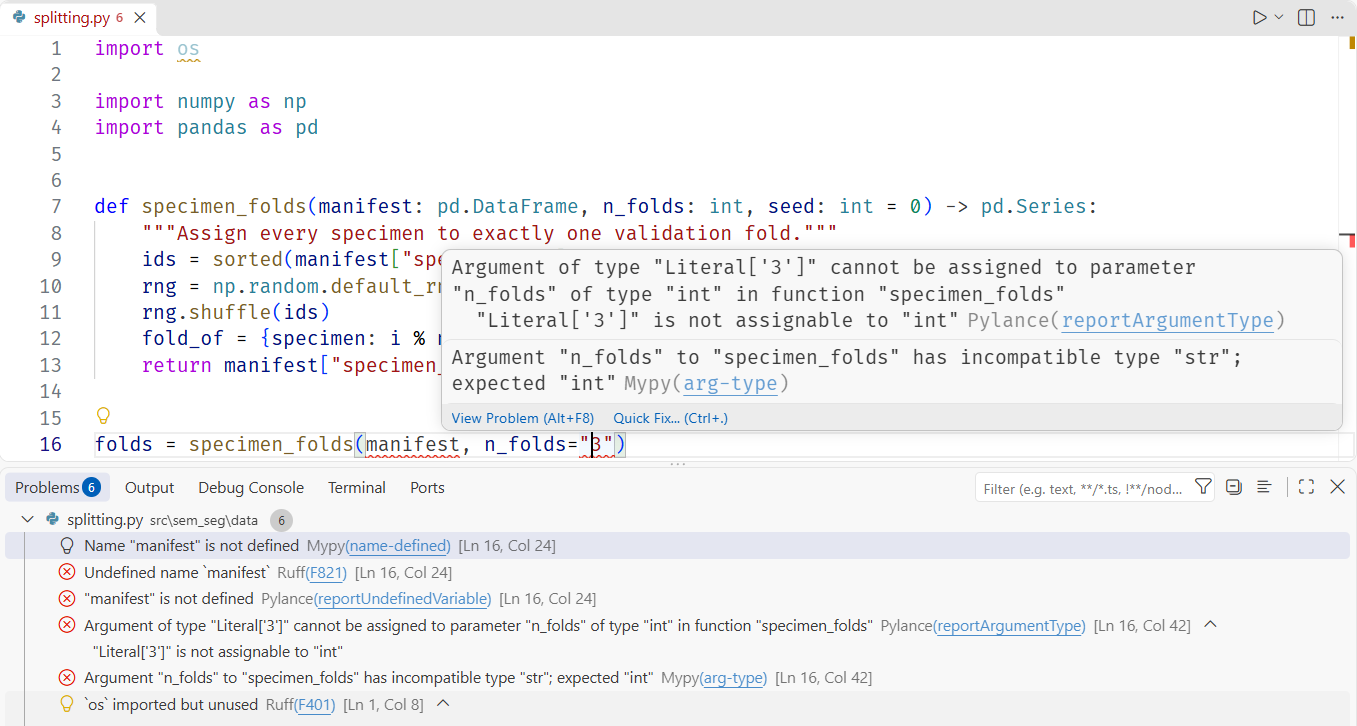
\includegraphics[width=\linewidth]{assets/screens/vscode-lint.png}};
        \begin{scope}[x={(img.south east)},y={(img.north west)}]
          \node[number mark] at (0.179,0.963) {1};
          \node[number mark] at (0.849,0.698) {2};
          \node[number mark] at (0.111,0.328) {3};
        \end{scope}
      \end{tikzpicture}
    \end{column}
    \begin{column}{0.27\textwidth}
      % each item numbered by its marker on the screenshot
      \footnotesize
      \begin{itemize}\setlength\itemsep{2mm}
        \item[\numbermark{1}] Ruff: unused import (\fn{F401}), undefined name (\fn{F821})
        \item[\numbermark{2}] Pylance and mypy: a string passed as \fn{n\_folds}
        \item[\numbermark{3}] Problems panel: every finding, with its tool and rule
      \end{itemize}
    \end{column}
  \end{columns}
  \note{\textbf{8:00--8:40}\par
    A real screenshot: VS Code 1.142 with the Ruff, Pylance and Mypy extensions on a
      deliberately broken version of our split function.\par
    Squiggles mark the unused import, the undefined name and the wrong argument type; hovering
      shows the message and which tool raised it.\par
    The Problems panel lists all six findings, each with its tool and rule, so you can look up
      or switch off a rule.\par
    The agent sees the same findings when it runs the tools from the terminal.}
\end{frame}

% ------------------------------------------------------------ set up once
\begin{frame}[fragile,source={Astral (2026), Ruff: editor setup · Microsoft (2026), Mypy Type Checker; Pylance README}]{Set them up once}
  % left: the tools on the command line; right: the same tools in VS Code. The right column is
  % wide enough for the longest line of settings.json (55 characters at 7 pt) on one line; the
  % left one then holds 42 characters of code and a table whose widest label is "Format".
  \begin{columns}[T,onlytextwidth]
    \begin{column}{0.425\textwidth}
\begin{codefile}[style=sh,basicstyle=\ttfamily\fontsize{7}{8.4}\selectfont]{pyproject.toml}
[tool.ruff]  # rules: Ruff's defaults
line-length = 100

[tool.mypy]
python_version = "3.12"
\end{codefile}
      \scriptsize\renewcommand\arraystretch{1.4}\setlength\tabcolsep{3pt}
      \begin{tabularx}{\linewidth}{@{}>{\bfseries}l>{\ttfamily}X@{}}
        \toprule
        Install        & conda install -c conda-forge ruff mypy\\
        \midrule
        Lint           & ruff check --fix\\
        Format         & ruff format\\
        Types          & mypy src\\
        \bottomrule
      \end{tabularx}
    \end{column}
    \begin{column}{0.545\textwidth}
\begin{codefile}[basicstyle=\ttfamily\fontsize{7}{8.4}\selectfont]{.vscode/settings.json}
{
  "[python]": {
    "editor.defaultFormatter": "charliermarsh.ruff",
    "editor.formatOnSave": true,
    "editor.codeActionsOnSave": {
      "source.fixAll": "explicit",
      "source.organizeImports": "explicit"}},
  "python.analysis.typeCheckingMode": "standard",
  "mypy-type-checker.importStrategy": "fromEnvironment"
}
\end{codefile}
      \footnotesize
      \begin{itemize}\setlength\itemsep{1mm}
        \item VS Code extensions: Python (brings Pylance), Ruff, Mypy Type Checker
        \item pick the environment: \emph{Python: Select Interpreter}
        \item the same commands go into \fn{AGENTS.md}
      \end{itemize}
    \end{column}
  \end{columns}
  \note{\textbf{8:40--9:40}\par
    Set up once per repository, then it runs by itself.\par
    The tool settings live in pyproject.toml, which works for conda projects too.\par
    One conda command installs both; by hand, three commands lint, format and type-check.\par
    In VS Code, install the Python extension, which brings Pylance, plus the Ruff and Mypy Type
      Checker extensions, and select the project's environment.\par
    The workspace settings make Ruff format and fix on every save, switch Pylance's type
      checking on, and make the Mypy extension use the mypy installed in the environment rather
      than the older copy it bundles.\par
    The same commands go into AGENTS.md, so the agent runs them too.}
\end{frame}

\section[Repository]{Preparing the repository}
\sectionframe{03}{Preparing the repository}
  {What can the repository tell the agent, so that we do not have to?}
  {\faFolderOpen}

% ------------------------------------------------------ the layout and its files
% Left: a standard layout, adapted from Cookiecutter Data Science, with one AGENTS.md. Right: the
% same repository later, its AGENTS.md split into three files. One picture, so that the arrow can
% run from one tree to the other: the rows are the theme's folder-tree rows, the pages are drawn
% here. Both trees start at the same height with a row pitch of 3.5 mm; the arrow leaves the
% AGENTS.md row on the left (row 9, y = -12.6 - 8 * 3.5) for rows 5 to 7 on the right.
\begin{frame}[source={DrivenData (2026), Cookiecutter Data Science}]{Setting up the repository}
  \begin{tikzpicture}[x=1mm,y=1mm,
      head/.style={anchor=north west,inner sep=0pt,font=\small\bfseries,text=udsdark},
      page/.style={draw=udsgreylight,fill=white,line width=0.5pt,rounded corners=1.2mm},
      split/.style={udsblue,line width=0.9pt},
      splitarrow/.style={split,-{Stealth[length=2mm,width=1.6mm]}}]
    \useasboundingbox (0,0) rectangle (144,-55);
    % ---- left: the layout, and a link to the template it follows
    \node[head] at (0,0) {A standard layout};
    \node[anchor=north west,inner sep=0pt,font=\footnotesize] at (0,-4.6)
      {\href{https://cookiecutter-data-science.drivendata.org/\#directory-structure}%
        {\faGlobe\enspace\underline{\fn{cookiecutter-data-science}}}};
    \draw[page] (0,-9.4) rectangle (60,-54.4);
    \begin{scope}[shift={(2.4,-12.6)}]
      \treestart{note at=30,row height=3.5}
      \tdir{0}{sem-seg/}{}
      \tdir{1}{data/raw/}{never edited}
      \tdir{1}{data/processed/}{made by the code}
      \tdir{1}{models/}{trained models}
      \tdir{1}{notebooks/}{exploring}
      \tdir{1}{reports/figures/}{figures for papers}
      \tdir{1}{src/sem\_seg/}{the code}
      \tdir{1}{tests/}{}
      \tfile{1}{\textcolor{udsblue}{\textbf{AGENTS.md}}}{\textcolor{udsblue}{for the agent}}
      \tfile{1}{environment.yml}{}
      \tfile{1}{pyproject.toml}{}
      \tfile{1}{README.md}{for people}
    \end{scope}
    % ---- right: the same repository once AGENTS.md has grown; what stays the same in grey
    \node[head] at (74,0) {As the project grows};
    \draw[page] (74,-9.4) rectangle (144,-40.3);
    \begin{scope}[shift={(76.4,-12.6)}]
      \treestart{note at=33.6,row height=3.5}
      \tdir{0}{sem-seg/}{}
      \tdirgrey{1}{data/ \dots}{as before}
      \tdirgrey{1}{models/ \dots\ reports/}{}
      \tdirgrey{1}{src/sem\_seg/, tests/}{}
      \tfile{1}{\textcolor{udsblue}{\textbf{AGENTS.md}}}{commands, rules, pointers}
      \tfile{1}{GLOSSARY.md}{the project's words}
      \tfile{1}{CODING\_STANDARDS.md}{how code is written here}
      \tfilegrey{1}{environment.yml, \dots}{}
    \end{scope}
    \node[anchor=north west,inner sep=0pt,font=\footnotesize,text=udsdark,text width=70mm,
      align=left] at (74,-43.4) {\fn{AGENTS.md} keeps what every session needs and points to
      the two new files};
    % ---- one file becomes three: from the AGENTS.md row on the left to rows 5 to 7 on the right
    \draw[split] (49.5,-40.6) -- (62,-40.6);% starts clear of the note "for the agent"
    \foreach \y in {-26.6,-30.1,-33.6} \draw[splitarrow] (62,-40.6) to[out=0,in=180] (74,\y);
  \end{tikzpicture}
  \note{\textbf{9:50--10:50}\par
    Before any file for the agent: a layout that people and agents already know.\par
    This one follows Cookiecutter Data Science, a template for data projects, with the code in
      src and its tests beside it: raw data that is never edited, processed data that the code
      makes, models, notebooks for exploring, figures for papers.\par
    An agent finds its way in it the way a new colleague does.\par
    At the root sits AGENTS.md, the one file written for the agent.\par
    As the project grows, AGENTS.md keeps what every session needs, and two files take the rest:
      GLOSSARY.md for the project's words, CODING\_STANDARDS.md for how code is written here.}
\end{frame}

% --------------------------------------------------------------- AGENTS.md
% The example file beside what such a file should hold and leave out, after the prompting guides
% of Anthropic and OpenAI (SOURCES.md)
\begin{frame}[fragile,source={Anthropic (2026), Prompting Claude Opus 5.5 · OpenAI (2026), Using GPT-6}]{\texttt{AGENTS.md}}
  \begin{columns}[T,onlytextwidth]
    \begin{column}{0.57\textwidth}
\begin{codefile}[basicstyle=\ttfamily\fontsize{7.2}{8.75}\selectfont]{AGENTS.md}
# sem-seg
## Setup and checks
- Environment: conda env `sem-seg`, activated beforehand
- Fast check (CPU, synthetic data): `pytest -q`
- Lint, types: `ruff check`, `mypy src` §\textcolor{udsred}{\sffamily\scriptsize\faArrowLeft\ after every edit}§
## Conventions
- Terms: `GLOSSARY.md` (specimen, micrograph, patch) §\smash{\textcolor{udsblue}{\faLink}}§
- Decisions: `docs/adr/` §\smash{\textcolor{udsblue}{\faLink}}§
- Lengths in micrometres; pixel size from metadata
## Boundaries
- Never write to `data/raw/`; use `data/processed/`
- No cluster jobs (`sbatch`): the queue is shared
- Ask before adding a dependency
## When you finish
- Report changed files, checks run, open assumptions
\end{codefile}
    \end{column}
    \begin{column}{0.40\textwidth}
      \begin{tikzpicture}[x=1mm,y=1mm,
          head/.style={anchor=north west,inner sep=0pt,font=\footnotesize\bfseries},
          item/.style={anchor=north west,inner sep=0pt,font=\footnotesize,text=udsdark},
          why/.style={anchor=north west,inner sep=0pt,font=\scriptsize,text=udsgrey}]
        \useasboundingbox (0,0) rectangle (57,-54);
        \node[head,text=testgreen] at (0,0) {Put in};
        \foreach \t [count=\i] in {{commands to set up, test and check},
            pointers to what the code cannot show,what needs your approval,
            {when it is done, and what to report},the reason behind a rule}
          \node[item] at (0,-0.7-\i*4.3) {\textcolor{testgreen}{\faCheck}\enspace\t};
        \node[head,text=udsred] at (0,-27.8) {Leave out};
        \foreach \t/\w [count=\i] in {{rules that clash or are out of date}/{the agent may stop and wait},
            {vague wishes: ``write clean code''}/{name the exact mistake instead},
            {``think carefully'', ``be thorough''}/{current models already do}} {
          \node[item] at (0,-25-\i*7.6) {\textcolor{udsred}{\faTimes}\enspace\t};
          \node[why] at (4.3,-28.8-\i*7.6) {\w};
        }
      \end{tikzpicture}
    \end{column}
  \end{columns}
  \note{\textbf{10:50--12:10}\par
    AGENTS.md is the one file that tools supporting it load at the start of every session.\par
    It holds what the agent cannot find out alone: the commands to set up, test and check; what
      the code cannot show, or which file shows it; what needs our approval; when the work is done
      and what to report.\par
    Fifteen lines, each preventing a specific mistake, and one says why: the cluster queue is
      shared.\par
    The checks of section 2 are here, so the agent runs them after every edit; the boundaries are
      requests, not locks.\par
    Today's models follow such files closely: OpenAI notes that its latest model is more
      sensitive to files such as AGENTS.md, and that unclear or conflicting guidance can make it
      stop early.\par
    So leave out rules that clash or are out of date; vague wishes such as write clean code,
      where naming the exact mistake works better; and lines such as think carefully, which
      Anthropic advises removing from system prompts, since the model decides how much to
      think.\par
    Keep it short, and review it like code.}
\end{frame}

% ---------------------------------------------------- glossary, standards
% \tagchip{text}: a tag naming what a file holds
\newcommand\tagchip[1]{\tikz[baseline=(t.base)]\node[draw=udsblue,fill=bluetint,line width=0.4pt,
  rounded corners=0.6mm,inner xsep=1mm,inner ysep=0.5mm,font=\scriptsize,text=udsdark] (t) {#1};}
\begin{frame}[fragile,source={Pocock (2026), mattpocock/skills v1.3.1: domain-modeling, code-review, retro}]{\texttt{GLOSSARY.md} and \texttt{CODING\_STANDARDS.md}}
  \begin{columns}[T,onlytextwidth]
    \begin{column}{0.485\textwidth}
      {\scriptsize\color{udsgrey}holds\enspace}\tagchip{term and meaning}\enspace
        \tagchip{words to avoid}\enspace\tagchip{code name}\par\vskip1.6mm
\begin{codefile}[basicstyle=\ttfamily\fontsize{7}{8.5}\selectfont]{GLOSSARY.md\enspace\textcolor{udsgreymid}{\sffamily\scriptsize read when pointed to}}
# Glossary
Specimen: one physical sample (`specimen_id`).
  Avoid: §\textcolor{udsred}{\bfseries sample}§, coupon. §\textcolor{udsred}{\sffamily\scriptsize\faArrowLeft\ the word in our request}§
Area: one imaged region of a specimen.
Micrograph: one SEM image of an area
  (`micrograph_id`). Avoid: image, frame.
Patch: a crop of a micrograph used in
  training (`patch_id`). Avoid: tile.
Fold: specimens held out together; every
  specimen belongs to exactly one fold.
\end{codefile}
    \end{column}
    \begin{column}{0.485\textwidth}
      {\scriptsize\color{udsgrey}holds\enspace}\tagchip{seeds}\enspace\tagchip{input checks}\enspace
        \tagchip{tests}\enspace\tagchip{paths}\par\vskip1.6mm
\begin{codefile}[basicstyle=\ttfamily\fontsize{7}{8.5}\selectfont]{CODING\_STANDARDS.md\enspace\textcolor{udsgreymid}{\sffamily\scriptsize read in review}}
# Coding standards
- Every random step takes a `seed`; the
  same seed gives the same result.
- Public functions check their inputs and
  raise `ValueError` naming the problem.
- Tests call public functions on small,
  hand-written fixtures, never real data.
- Expected values come from the fixture,
  never recomputed the way the code does.
- Paths come from `config.py`, never
  written into a function.
\end{codefile}
    \end{column}
  \end{columns}
  \note{\textbf{12:10--13:30}\par
    Two files the agent reads only when something points to them.\par
    A glossary holds the project's terms: what each one means, the words to avoid and the name the
      code uses for it; our request said sample, and here sample is a word to avoid.\par
    The clarifying step of section 7 writes terms into it as soon as they are agreed.\par
    Coding standards hold the rules a reviewer checks: seeds, input checks, how tests are built,
      where paths come from; a fixture is the small, hand-made input a test runs on.\par
    In the workflow of section 7 the review step reads it, not the implementing agent, which
      already carries the most context.\par
    Rules that a linter can check belong in Ruff's settings instead, so that every run checks
      them.}
\end{frame}

\section[Decisions]{Architecture Decision Records (ADRs)}
\sectionframe{04}{Architecture Decision Records (ADRs)}
  {Why does the project work this way, and what if we change our minds?}
  {\faBalanceScale}

% ------------------------------------------------------------ what / when
\begin{frame}[source={Nygard (2011), Documenting architecture decisions · Pocock (2026), mattpocock/skills v1.3.1, domain-modeling}]{What an ADR is, and when to write one}
  \begin{tikzpicture}[x=1mm,y=1mm,
      crit/.style={inner sep=0pt,font=\footnotesize,text=udsdark,align=center},
      item/.style={anchor=base west,inner sep=0pt,font=\footnotesize,text=udsdark}]
    % the record itself: Nygard's format
    \node[anchor=north west,inner sep=0pt,font=\footnotesize,text=udsdark] at (0,0)
      {\textbf{One decision per record:}\enspace title · context · decision · status ·
       consequences; numbered; superseded records stay};
    % write one only where all three hold; each label sits in its circle's own part
    \coordinate (A) at (17,-22); \coordinate (B) at (35,-22); \coordinate (C) at (26,-37.6);
    \foreach \p in {A,B,C}
      \filldraw[draw=udsblue,line width=0.7pt,fill=udsblue,fill opacity=0.09] (\p) circle (15);
    \node[crit] at (11.5,-19.5) {hard to\\reverse};
    \node[crit] at (40.5,-19.5) {surprising\\without\\context};
    \node[crit] at (26,-44) {a real\\trade-off};
    \node[inner sep=0.4mm,font=\small\bfseries,text=udsred] (adr) at (26,-27.2) {ADR};
    % where all three usually hold in research code, level with the circles' top
    \node[anchor=north west,inner sep=0pt,font=\footnotesize\bfseries,text=udsdark] at (70,-7)
      {typical in research code};
    \foreach \t [count=\i] in {the split unit and the evaluation protocol,merged or remapped classes,
        {units, scales, normalisation},the metric that decides what is ``better''}
      \node[item] at (72,-9.2-\i*5.4) {\textcolor{udsred}{\faAngleRight}\enspace\t};
    \draw[udsred,line width=0.6pt] (adr.east) to[out=0,in=180] (69.4,-21.7);
    \node[anchor=base west,inner sep=0pt,font=\scriptsize,text=udsgrey] at (72,-41)
      {no ADR: plot styling, renames};
  \end{tikzpicture}
  \note{\textbf{13:40--14:40}\par
    An architecture decision record keeps one decision with its reasons.\par
    Nygard's format: title, context, decision, status and consequences, including the bad
      ones.\par
    Records are numbered in sequence, numbers are never reused, and a superseded record stays in
      the repository.\par
    A useful test, from the skills of section 7: write one only when the decision is hard to
      reverse, would surprise a newcomer, and came from a real trade-off.\par
    In research code that is usually about what a number means: the split unit, class
      definitions, units and normalisation, the metric.\par
    Plot styling and renames do not need one.}
\end{frame}

% ------------------------------------------------------------- ADR example
\begin{frame}[fragile]{ADR-0003: specimen-level splits}
  \begin{columns}[T,onlytextwidth]
    \begin{column}{0.58\textwidth}
\begin{codefile}[basicstyle=\ttfamily\fontsize{7}{8.4}\selectfont]{docs/adr/0003-specimen-level-splits.md}
# ADR-0003: Specimen-level splits
Status: accepted. Supersedes ADR-0001 (random patch split).
## Context
Micrographs of one specimen share preparation and etching;
several show the same area. A random patch split puts this
material in training and validation.
## Decision
Specimens are assigned to validation folds; each patch
inherits its specimen's fold. Folds are saved with seed
and manifest hash and checked for overlap.
## Considered options
Random patch split; split by micrograph. Both leak.
## Consequences
Few independent units: report every fold and its spread.
One specimen per state: a held-out specimen is a new state.
\end{codefile}
    \end{column}
    \begin{column}{0.39\textwidth}
      \begin{tikzpicture}[x=1mm,y=1mm]
        \node[artifact,anchor=north west,text width=50mm,align=left,font=\scriptsize] (a1) at (0,0)
          {\texttt{0001-random-patch-split.md}\\[0.4mm]
           \textcolor{udsred}{Status: superseded by ADR-0003}};
        \node[artifact,anchor=north west,text width=50mm,align=left,font=\scriptsize,draw=udsblue,fill=bluetint] (a3) at (0,-16)
          {\texttt{0003-specimen-level-splits.md}\\[0.4mm]
           \textcolor{udsblue}{Status: accepted}};
        \draw[flow] (a3.north) -- node[lbl,right]{supersedes} (a1.south);
        \node[anchor=north west,text width=54mm,font=\scriptsize,inner sep=0pt] at (0,-27.5)
          {ADR-0001 stays: it shows what was tried and why it changed.};
      \end{tikzpicture}\par\vskip3mm
      \begin{panel}[fontupper=\footnotesize,colback=bluetint,borderline west={1.2mm}{0pt}{udsblue},left=3.5mm]
        An agent chasing a better score finds ADR-0003 through \fn{AGENTS.md} before it brings back a
        random split.
      \end{panel}
    \end{column}
  \end{columns}
  \note{\textbf{14:40--15:40}\par
    The record for our running example.\par
    The context explains why a random patch split misleads here; the decision is short and
      testable; the considered options show that splitting by micrograph was rejected for the
      same reason.\par
    The consequences are honest: few specimens mean few independent units, and with one specimen
      per material state every held-out specimen is also a new state.\par
    ADR-0001 is not deleted; its status points to its successor.\par
    An agent tuning for a better score finds this record before it undoes the decision.}
\end{frame}

% ------------------------------------------------------------- file roles
\begin{frame}[source={OpenAI (2026), Custom instructions with AGENTS.md · Pocock (2026), mattpocock/skills v1.3.1: code-review; v1.3 changelog}]{When the agent reads each file}
  % the files of sections 3 and 4, the README and the task specification of section 1, placed on
  % an agent session at the moment each one is read
  \begin{tikzpicture}[x=1mm,y=1mm,
      chip/.style={draw=udsgreylight,fill=white,rounded corners=0.6mm,inner xsep=1mm,inner ysep=0.8mm,
        anchor=north west,font=\ttfamily\fontsize{7.4}{8.4}\selectfont,text=udsdark,line width=0.5pt,
        path picture={\draw[udsblue,line width=0.9pt] (path picture bounding box.north west)
          -- (path picture bounding box.north east);}},
      always/.style={chip,draw=udsblue,line width=0.9pt},
      ondemand/.style={chip,dashed,draw=udsdark,path picture={}},
      reviewstep/.style={chip,draw=udsblue,fill=bluetint,path picture={},font=\footnotesize},
      say/.style={anchor=north west,inner sep=0pt,font=\scriptsize,text=udsdark,align=left,text width=30mm,
        execute at begin node={\hyphenpenalty=10000\raggedright}},
      drop/.style={udsgreymid,line width=0.5pt},
      dot/.style={circle,fill=udsdark,inner sep=0pt,minimum size=1.8mm}]
    % AGENTS.md points to the glossary and the ADRs
    \node[always] (ag) at (0,-4.6) {AGENTS.md};
    \node[ondemand] (gl) at (44,-4.6) {GLOSSARY.md};
    \node[ondemand] (ad) at (78,-4.6) {docs/adr/};
    \draw[drop,dashed] (ag.north) |- (ad.north |- 0,-1.6);
    \foreach \n in {gl,ad} \draw[drop,dashed,-{Stealth[length=1.6mm,width=1.2mm]}] (\n.north |- 0,-1.6) -- (\n.north);
    \node[anchor=south,inner sep=0.5mm,font=\scriptsize,text=udsgrey,fill=white] at (27,-1.6) {points to};
    \node[say] at ([yshift=-1.2mm]ag.south west) {\textcolor{udsblue}{\bfseries every session}\\ commands, boundaries, pointers};
    \node[say] at ([yshift=-1.2mm]gl.south west) {\textbf{when pointed to}\\ domain terms};
    \node[say] at ([yshift=-1.2mm]ad.south west) {\textbf{when pointed to}\\ one decision and its reasons};
    % read in review
    \node[chip] (cs) at (112,-4.6) {CODING\_STANDARDS.md};
    \node[say] at ([yshift=-1.2mm]cs.south west) {\textbf{in review}\\ how code is written here};
    % the session, left to right, and where each file enters it
    \draw[flow,line width=0.9pt] (0,-27) -- (143.4,-27);% the tip stays inside the text width
    \node[anchor=south west,inner sep=0.6mm,font=\scriptsize,text=udsgrey] at (12,-27) {an agent session};
    \foreach \n in {ag,gl,ad,cs} {\node[dot] at (\n.south |- 0,-27) {}; \draw[drop] (\n.south |- 0,-21.6) -- (\n.south |- 0,-27);}
    % the task's own specification comes with it; the review checks the code against the standards
    \node[chip,font=\footnotesize] (sp) at (0,-32) {task specification};
    \node[say] at ([yshift=-1.2mm]sp.south west) {\textbf{with the task}\\ objective, acceptance criteria};
    \draw[drop] (ag.south |- 0,-27) -- (ag.south |- sp.north);
    \node[reviewstep] (cr) at (112,-32) {\faSearch\enspace review};
    \node[say] at ([yshift=-1.2mm]cr.south west) {a person or an agent checks the code against it};
    \draw[drop] (cs.south |- 0,-27) -- (cs.south |- cr.north);
    % read like any other file
    \node[chip,draw=udsgreylight,text=udsgrey,path picture={}] (rd) at (44,-34) {README.md};
    \node[say,text=udsgrey,text width=40mm,anchor=west] at ([xshift=2mm]rd.east) {for people; read like any other file};
  \end{tikzpicture}
  \note{\textbf{15:40--16:30}\par
    Each file on one agent session, at the moment it is read.\par
    AGENTS.md at the start of every session; the glossary and the ADRs when AGENTS.md points to
      them.\par
    The task specification of section 1 comes with the task; the coding standards are read when
      the change is reviewed, by a person or an agent.\par
    The README is for people; the agent reads it like any other file.\par
    Keep each fact in one place and link to it: copies go stale.}
\end{frame}

% ------------------------------------ the specification of section 1, remembered
% Slide 5's five cards again, greyed: the theme's colours are redefined for one group only, so the
% same macros draw them. A stamp repeats slide 5's warning; the strip says where the parts that
% repeat are now, which the next slide shows card by card.
\begin{frame}{Remember the bounded task specification?}
  \begin{tikzpicture}[x=1mm,y=1mm]
    \useasboundingbox (0,0) rectangle (144,-54);
    \begingroup
      \colorlet{udsblue}{udsgreymid}\colorlet{udsdark}{udsgreymid}
      \foreach \k/\l in {0/Objective,1/Context,2/Constraints,3/Acceptance,4/Verification}
        {\speccard{\k}{0}{-41.4}{\l}{udsgreypale!60}}
      \foreach \k/\t in {
          0/{add \fn{specimen\_folds()} to \fn{src/sem\_seg/\allowbreak data/\allowbreak splitting.py}; use it
            in the training CLI as \fn{--split specimen}},
          1/{``sample'' means specimen: one physical sample, column \fn{specimen\_id} of the manifest},
          2/{leave \fn{data/raw/} and the manifests unchanged; no new dependencies; no GPU jobs},
          3/{each specimen in exactly one fold; each patch inherits its specimen's fold; same seed, same
            folds; \fn{ValueError} if \fn{specimen\_id} is missing or there are fewer specimens than folds},
          4/{\fn{pytest tests/data -q} passes; report changed files, test output and assumptions}}
        \node[spec body] at (b\k) {\t};
    \endgroup
    % slide 5's warning, stamped across the cards
    \node[rotate=7,draw=udsred,double=white,double distance=0.7pt,line width=0.8pt,
      rounded corners=1mm,fill=white,fill opacity=0.88,text opacity=1,text=udsred,
      font=\large\bfseries,inner xsep=3mm,inner ysep=2.2mm] at (72,-21)
      {\faExclamationTriangle\enspace too much to write for every task};
    % where those parts are now
    \fill[bluetint] (0,-48.4) rectangle (144,-54);
    \fill[udsblue] (0,-48.4) rectangle (1.2,-54);
    \node[anchor=west,inner sep=0pt,font=\footnotesize,text=udsdark] at (3.6,-51.2)
      {\textcolor{udsblue}{\faCheck}\enspace what repeats is now in files: \fn{AGENTS.md},
       \fn{GLOSSARY.md}, ADRs, \fn{CODING\_STANDARDS.md}};
  \end{tikzpicture}
  \note{\textbf{16:30--17:00}\par
    Remember the bounded specification from the start of the talk.\par
    Every part of it was written by hand, for every task: what a specimen is, which data must not
      change, how to run the tests, what to report.\par
    That is the part that repeats, and it now lives in the files of sections 3 and 4.}
\end{frame}

% ------------------------------------------------ the request, revisited
\begin{frame}{The same request, in a prepared repository}
  \begin{tikzpicture}[x=1mm,y=1mm]
    % the cards fill the text width exactly; strokes on their edges must not widen the picture
    \useasboundingbox (0,0) rectangle (144,-54);
    \specterminal{0}{the request}
    \node[spec request] at (term) {> Add validation folds by specimen to the training CLI, as decided in ADR-0003.};
    \node[anchor=west,inner sep=0pt,font=\scriptsize\bfseries,text=udsdark] at (0,-15.8)
      {where the rest comes from};
    % the same five cards as on slides 4 and 5: the objective is the request itself, every other
    % part now comes from files
    \speccard{0}{-19}{-44.4}{Objective}{darktint}
    \foreach \k/\l in {1/Context,2/Constraints,3/Acceptance,4/Verification}
      {\specfilecard{\k}{-19}{-44.4}{\l}{darktint}}
    \node[spec chip,draw=termbg,fill=termbg,text=termfg,path picture={}] at (b0) {\faTerminal\ the request};
    % context
    \node[spec chip] (c1) at (b1) {GLOSSARY.md};
    \node[spec note] (c1s) at ([yshift=-0.8mm]c1.south west) {specimen, fold};
    \node[spec chip] (c2) at ([yshift=-2.2mm]c1s.south west) {ADR-0003};
    \node[spec note] at ([yshift=-0.8mm]c2.south west) {why; how folds are saved};
    % constraints
    \node[spec chip] (k1) at (b2) {AGENTS.md};
    \node[spec note] at ([yshift=-0.8mm]k1.south west) {boundaries};
    % acceptance
    \node[spec chip] (a1) at (b3) {ADR-0003};
    \node[spec note] (a1s) at ([yshift=-0.8mm]a1.south west) {one fold per specimen};
    \node[spec chip] (a2) at ([yshift=-2.2mm]a1s.south west) {CODING\_STANDARDS.md};
    \node[spec note] at ([yshift=-0.8mm]a2.south west) {seed, input checks};
    % verification
    \node[spec chip] (v1) at (b4) {AGENTS.md};
    \node[spec note] at ([yshift=-0.8mm]v1.south west) {fast check, report};
    % what the files leave open, the agent has to ask: the clarifying step of section 7
    \node[anchor=west,inner sep=0pt,font=\scriptsize,text=udsred] at (0,-49.4)
      {\faQuestionCircle\enspace still open: what no file says, e.g.\ the default number of folds};
  \end{tikzpicture}
  \note{\textbf{17:00--18:00}\par
    Now the same request, in the repository we prepared.\par
    With these files in place, one sentence in the project's language is enough.\par
    Four of the five parts now come from files; only the objective is in the request.\par
    The glossary says what a specimen and a fold are.\par
    ADR-0003 says why folds go by specimen and how they are saved.\par
    AGENTS.md carries the boundaries, the test command and what to report.\par
    CODING\_STANDARDS.md makes seeds and input checks part of every review.\par
    What the files leave open, here the default number of folds, is what the clarification step
      of section 7 asks.\par
    This works only while AGENTS.md points to the files and they are kept current.}
\end{frame}

\section[Version control]{Version control with git}
\sectionframe{05}{Version control with git}
  {How do we keep every version, and see exactly what an agent changed?}
  {\faCodeBranch}

% ------------------------------------------------------------- what it is
\begin{frame}[source={Chacon \& Straub (2014), Pro Git, 2nd ed., git-scm.com/book}]{Version control: one folder, every version}
  \begin{columns}[T,onlytextwidth]
    \begin{column}{0.34\textwidth}
      \begin{ablock}[equal height group=vc,fontupper=\footnotesize]{Without}
        {\ttfamily\footnotesize splitting.py\\ splitting\_old.py\\ splitting\_v2\_final.py\\
         splitting\_v2\_final\_FIXED.py\\ results\_new2/\par}\vskip2mm
        Which version produced figure 3?
      \end{ablock}
    \end{column}
    \begin{column}{0.62\textwidth}
      \begin{dblock}[equal height group=vc,fontupper=\footnotesize]{With git}
        \centering
        \begin{tikzpicture}[x=1mm,y=1mm,
            commit/.style={circle,draw=udsblue,fill=white,line width=0.9pt,minimum size=3mm,inner sep=0pt},
            bcommit/.style={commit,draw=udsred},
            msg/.style={font=\scriptsize,text=udsdark,inner sep=0.6mm}]
          \draw[udsblue,line width=1pt] (0,0) -- (51,0);
          \draw[udsred,line width=1pt] (14,0) to[out=0,in=180] (23,9) -- (42,9) to[out=0,in=180] (51,0);
          \foreach \n/\x/\t in {a/0/random split,b/14/checks,m/51/merge} {
            \node[commit] (\n) at (\x,0) {};
            \node[msg,anchor=north] at (\n.south) {\t};
          }
          \foreach \n/\x/\t in {e/25/specimen folds,f/40/tests} {
            \node[bcommit] (\n) at (\x,9) {};
            \node[msg,anchor=south] at (\n.north) {\t};
          }
          \node[font=\scriptsize\bfseries,text=udsblue,anchor=east] at (-2.5,0) {main};
        \end{tikzpicture}\par\vskip1.5mm
        \raggedright\renewcommand\arraystretch{1.15}\setlength\tabcolsep{3pt}
        \begin{tabular}{@{}>{\bfseries}l l@{}}
          commit & a snapshot with a message, an author and a date\\
          diff   & what changed between two snapshots\\
          \textcolor{udsred}{branch} & a separate line of work, merged when ready\\
          remote & a copy on a server (GitHub): backup, sharing, review\\
        \end{tabular}
      \end{dblock}
    \end{column}
  \end{columns}
  \note{\textbf{18:10--19:20}\par
    Many of us keep versions as copies: splitting old, v2, final, fixed.\par
    After a few months nobody knows which copy produced a figure.\par
    Version control replaces the copies with one folder and its history.\par
    Git stores a snapshot of the project each time you commit, with a message, an author and a
      date; a diff shows what changed between two snapshots.\par
    A branch is a separate line of work, for an experiment or for an agent's task, merged back
      when it is ready.\par
    A remote such as GitHub holds a copy of the history on a server: a backup, a way to share,
      and the place where changes are reviewed.\par
    There a branch comes back as a pull request: a request to merge it, with its diff open for
      review before it reaches main.}
\end{frame}

% ------------------------------------------------------- learning curve
\begin{frame}[fragile,source={Chacon \& Straub (2014), Pro Git, 2nd ed., git-scm.com/book · Microsoft (2026), VS Code docs: Source control}]{Getting started takes five commands}
  \edef\colgap{\the\dimexpr0.04\textwidth\relax}
  \begin{columns}[T,onlytextwidth]
    \begin{column}{0.55\textwidth}
\begin{terminal}[basicstyle=\ttfamily\fontsize{7.2}{9.2}\selectfont]{terminal}
$ git init              # once: start the history
$ git status            # what has changed?
$ git add src/ tests/   # choose what goes in
$ git commit -m "Split by specimen"
$ git push              # copy it to GitHub
\end{terminal}
      \vskip1mm
\begin{codefile}[style=sh,basicstyle=\ttfamily\fontsize{7.2}{9.2}\selectfont]{.gitignore}
data/          # raw and derived data stay out
.venv/         # environments are rebuilt, not stored
*.ckpt         # model checkpoints
.env           # secrets
.claude/worktrees/  # agent worktrees
\end{codefile}
    \end{column}
    \begin{column}{0.41\textwidth}
      \begin{tikzpicture}
        \node[anchor=south west,inner sep=0pt,draw=udsgreylight,line width=0.4pt] (img) at (0,0)
          {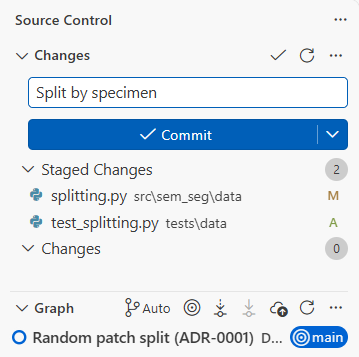
\includegraphics[height=36mm]{assets/screens/vscode-scm.png}};
        % each control, labelled with the command it replaces; push is the cloud button of the
        % graph's title row, so its line starts under that button and passes below the row
        \begin{scope}[x={(img.south east)},y={(img.north west)},
            cmd/.style={right,inner sep=0.6mm,font=\ttfamily\scriptsize,text=udsdark}]
          \foreach \y/\t in {0.683/commit,0.521/add,0.412/status}
            \draw[udsgreymid,line width=0.5pt] (1,\y) -- ++(2.5mm,0) node[cmd] {git \t};
          \draw[udsgreymid,line width=0.5pt] (0.79,0.112) |- (1,0.1) -- ++(2.5mm,0)
            node[cmd] {git push};
        \end{scope}
      \end{tikzpicture}\par\vskip1mm
      {\scriptsize VS Code's Source Control panel does the same with clicks.\par}\vskip2mm
      % the arrow spans the gap between the columns (0.04 of the text width), so it starts at the
      % edge of .gitignore; drawn by the box itself, it also lands right in the notes thumbnails
      \begin{panel}[colback=redtint,borderline west={1.2mm}{0pt}{udsred},left=3.5mm,fontupper=\footnotesize,
          overlay={\draw[flow] ([xshift=-\colgap]frame.west) -- (frame.west);}]
        data, environments and secrets do not belong in the history
      \end{panel}
    \end{column}
  \end{columns}
  \note{\textbf{19:20--20:20}\par
    The learning curve is shorter than its reputation.\par
    Five commands cover daily use: start the history once, check what changed, choose what goes
      into the next snapshot, commit it with a message, and push it to GitHub, the remote of the
      last slide.\par
    VS Code's Source Control panel does the same with buttons: here two files are staged, the
      message is typed, one click on Commit, and the cloud button pushes; the graph below is the
      history.\par
    The first push needs a repository on GitHub to push to; that cloud button, Publish Branch,
      creates one and pushes.\par
    A .gitignore file keeps out what does not belong in the history: data, environments, which
      are rebuilt from their description, model checkpoints, secrets, and the worktrees that Claude
      Code creates.\par
    Branches and merges can come later.}
\end{frame}

% ------------------------------------------------------- git and agents
\begin{frame}[source={OpenAI (2026), Agent approvals and security; Non-interactive mode · Anthropic (2026), Claude Code checkpointing}]{Why an agent needs version control}
  \begin{columns}[T,onlytextwidth]
    \begin{column}{0.66\textwidth}
      \begin{tikzpicture}
        \node[anchor=south west,inner sep=0pt,draw=udsgreylight,line width=0.4pt] at (0,0)
          {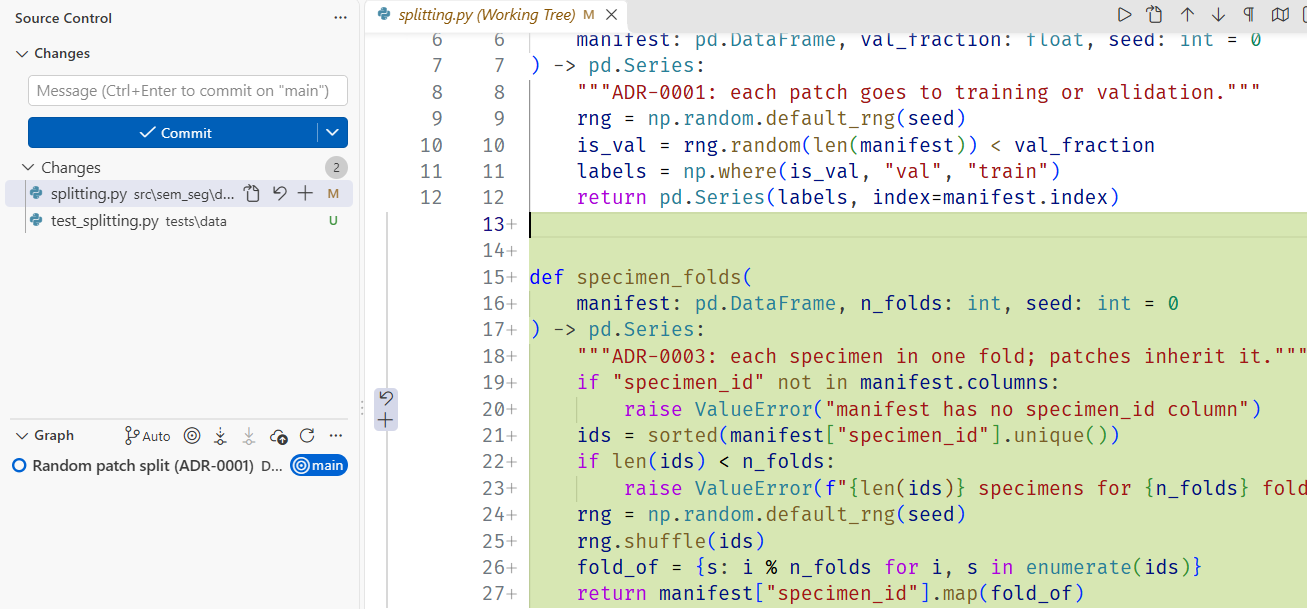
\includegraphics[width=\linewidth]{assets/screens/vscode-git.png}};
      \end{tikzpicture}\par\vskip1mm
      {\scriptsize An agent's change in VS Code's Source Control view: two files, every new line in green.\par}
    \end{column}
    \begin{column}{0.31\textwidth}
      \begin{tikzpicture}[x=1mm,y=1mm,
          commit/.style={circle,draw=udsblue,fill=white,line width=0.9pt,minimum size=3.4mm,inner sep=0pt},
          gitstep/.style={anchor=base west,inner sep=0pt,font=\footnotesize,text=udsdark,align=flush left,
            text width=38.6mm}]
        \useasboundingbox (0,0) rectangle (44.6,-52);
        % a checkpoint, the agent's uncommitted edits, then keep or discard them;
        % each label's first baseline sits 1 mm below its circle's centre
        \draw[udsblue,line width=0.9pt] (1.7,-1.9) -- (1.7,-14.4);
        \node[commit] at (1.7,-1.9) {};
        \node[gitstep] at (6,-2.9) {\textbf{checkpoint}\\commit before the agent starts};
        \node[commit,draw=udsred,dashed] (e) at (1.7,-14.4) {};
        \node[gitstep] at (6,-15.4) {\textbf{the agent's edits}\\read the diff, not the summary};
        \draw[udsblue,line width=0.9pt] (e.south) to[out=-90,in=180] (6,-27);
        \node[commit] at (7.7,-27) {};
        \node[gitstep,text width=33mm] at (11.6,-28)
          {\textbf{keep}\enspace\fn{git commit}\\{\color{udsgrey}undo later: \fn{git revert}}};
        \draw[udsgreymid,line width=0.9pt,dashed] (e.south) to[out=-90,in=180] (6,-38.6);
        \node[circle,fill=udsgreymid,text=white,inner sep=0pt,minimum size=3.4mm,font=\tiny]
          at (7.7,-38.6) {\faTimes};
        \node[gitstep,text width=33mm] at (11.6,-39.6)
          {\textbf{discard}\enspace\fn{git restore}\\{\color{udsgrey}the edits are lost}};
        \node[gitstep,text width=44.6mm,font=\footnotesize\bfseries,text=udsblue] at (0,-50.4)
          {one branch or worktree per task};
      \end{tikzpicture}
    \end{column}
  \end{columns}
  \note{\textbf{20:20--21:30}\par
    With git, an agent's work becomes a diff we can read before we accept it.\par
    Commit before the agent starts, so there is a checkpoint to return to.\par
    Read the diff itself, not the agent's summary of it: here, two files, every added line in
      green.\par
    Undo is one command: restore discards uncommitted changes for good, revert undoes a commit
      and keeps the history.\par
    A branch, or a separate worktree, per task keeps an agent's work apart from ours until it is
      reviewed.\par
    The tools assume all this.\par
    Codex checks at launch whether the folder is under version control, suggests read-only mode
      when it is not, and codex exec refuses to run outside a repository unless told
      otherwise.\par
    Claude Code can rewind its own file edits, but not files changed by shell commands, and its
      documentation says to keep using git.\par
    The workflow of section 7 commits each finished piece of work, and its review compares
      against a commit.}
\end{frame}

% ------------------------------------------------------------- worktrees
\begin{frame}[fragile,source={git documentation (2026), git-worktree · Anthropic Academy (2026)}]{Worktrees: work in parallel, merge when done}
  % the drawing carries the ideas; what a worktree is and its three commands sit beside it, level
  % with its middle
  \begin{columns}[c,onlytextwidth]
    \begin{column}{0.34\textwidth}
      \footnotesize
      \begin{itemize}\setlength\itemsep{1.5mm}
        \item a worktree: another folder of the same repository, on its own branch
        \item all folders share one history, so each branch merges into \fn{main}
      \end{itemize}\vskip2.5mm
\begin{terminal}[basicstyle=\ttfamily\fontsize{7.2}{8.5}\selectfont]{terminal}
$ git worktree add ../folds \
    -b agent/folds
$ git worktree list
$ git worktree remove ../folds
\end{terminal}
    \end{column}
    \begin{column}{0.63\textwidth}
      \centering
      \begin{tikzpicture}[x=1mm,y=1mm,
          pill/.style={rounded corners=2mm,minimum height=4mm,inner xsep=2mm,inner ysep=0.4mm,
            font=\fontsize{7}{8}\selectfont\bfseries,text=white},
          dot/.style={circle,inner sep=0pt,minimum size=2.4mm},
          tie/.style={udsgreylight,dashed,line width=0.5pt},
          card/.style={draw=udsblue,fill=bluetint,line width=0.6pt,rounded corners=1mm,
            align=left,font=\scriptsize,inner xsep=1.6mm,inner ysep=1.2mm}]
        % branches first, so that dots and cards sit on top of them
        \draw[udsblue,line width=1pt] (68,3) to[out=135,in=270] (55,20) to[out=90,in=235] (68,31);
        \draw[udsblue,line width=1pt] (68,3) to[out=162,in=270] (27,20) to[out=90,in=200] (68,42);
        \draw[udsdark,line width=1.2pt,-{Stealth[length=2.4mm,width=1.8mm]}] (68,0) -- (68,46);
        % your own folder, on main
        \node[card,draw=udsred,fill=redtint,anchor=south] at (68,46.6)
          {{\color{udsred}\faFolderOpen}\ \textbf{\fn{sem-seg/}}\quad\faCodeBranch\ \fn{main}\quad\faUser\ you};
        % commits on main, on the right; the two merges in red
        \foreach \y/\t/\c in {3/commit/udsdark,14/your commit/udsdark,31/merge/udsred,42/merge/udsred} {
          \node[dot,fill=\c] at (68,\y) {};
          \draw[tie] (69.5,\y) -- (72,\y);
          \node[pill,fill=\c,anchor=west] at (72,\y) {\t};
        }
        % one worktree per branch: its folder, its branch, its agent
        \foreach \x/\n/\b in {55/1/folds,27/2/check} {
          \node[dot,fill=udsblue] at (\x,20) {};
          \draw[tie] (\x-1.5,20) -- (\x-3,20);
          \node[card,anchor=east] at (\x-3,20)
            {{\color{udsblue}\faFolderOpen}\ \textbf{\fn{../\b}}\\ \faCodeBranch\ \fn{agent/\b}\\ \faRobot\ agent \n};
        }
      \end{tikzpicture}
    \end{column}
  \end{columns}
  \note{\textbf{21:30--22:30}\par
    A worktree is a second working folder of the same repository, checked out on its own
      branch.\par
    Each card is one: a folder next to the repository, its branch, and the agent working in it;
      your own folder, sem-seg, is the main worktree on main.\par
    Both agents start from the same commit on main and work at the same time, while you keep
      committing on main in your own folder.\par
    When an agent's work is reviewed, its branch is merged into main: first one, then the
      other.\par
    All worktrees share one history, and git lets a branch be checked out in only one worktree
      at a time, so the agents get in neither each other's way nor yours.\par
    Three commands: add creates the folder and the branch, list shows them, remove deletes the
      folder once its branch is merged.}
\end{frame}

% ------------------------------------------- worktrees in the app and the terminal
\begin{frame}[source={Anthropic (2026), Claude Code docs: Desktop; Worktrees; CLI reference}]{How to use worktrees?}
  \begin{tikzpicture}[x=1mm,y=1mm,
      head/.style={anchor=north west,inner sep=0pt,font=\small\bfseries,text=udsdark},
      stage/.style={circle,fill=udsblue,text=white,inner sep=0pt,minimum size=5.6mm,font=\scriptsize},
      txt/.style={anchor=north west,inner sep=0pt,font=\footnotesize,text=udsdark,align=flush left,
        text width=61mm},
      mono/.style={anchor=west,inner sep=0pt,font=\ttfamily\fontsize{7}{8}\selectfont}]
    \useasboundingbox (0,0) rectangle (144,-55);
    \node[head] at (8,0) {Claude app};
    \node[head] at (83,0) {Terminal};
    \draw[udsgreylight,line width=0.4pt] (72,0) -- (72,-54.6);
    % the app: Worktree on under the prompt box (screenshot), with a red box on the button
    \node[anchor=north west,inner sep=0pt,draw=udsgreylight,line width=0.4pt] (app) at (8,-4.6)
      {
\includegraphics[width=61mm]{assets/screens/claude-app-worktree.png}};
    \begin{scope}[shift={(app.south west)},x={($(app.south east)-(app.south west)$)},
        y={($(app.north west)-(app.south west)$)}]
      \draw[udsred,line width=1.1pt] (0.552,0.01) rectangle (0.809,0.35);
    \end{scope}
    % the terminal: the session's own branch, as Claude Code shows it
    \fill[termbg,rounded corners=1.2mm] (83,-4.6) rectangle (144,-19.04);
    \foreach \c [count=\i] in {termdot1,termdot2,termdot3} \fill[\c] (83.4+\i*2.3,-7.2) circle (0.7);
    \node[inner sep=0pt,font=\ttfamily\fontsize{7}{8}\selectfont,text=termdim] at (113.5,-7.2)
      {claude --worktree specimen-folds};
    \draw[white!18!termbg,line width=0.4pt] (83,-9.8) -- (144,-9.8);
    \node[mono,text=termfg] at (85.6,-12.9) {! git branch --show-current};
    \node[mono,text=termfg] at (85.6,-16.4) {\phantom{! }└ worktree-specimen-folds};
    \draw[udsred,line width=1.1pt] (84.6,-10.9) rectangle (124.4,-18.4);
    \node[anchor=north west,inner sep=0pt,font=\scriptsize,text=udsgrey] at (8,-20.6)
      {\textbf{Worktree}: ``Work in an isolated copy of the repository''};
    \node[anchor=north west,inner sep=0pt,font=\scriptsize,text=udsgrey] at (83,-20.6)
      {the session runs on its own branch};
    % one session, start to end: the same four stages, with their icons, in both columns
    \foreach \x in {2.8,77.8} {
      \draw[udsgreylight,line width=1.2pt] (\x,-28.7) -- (\x,-51.5);
      \foreach \y/\icon in {-28.7/\faPlay,-36.3/\faFolderOpen,-43.9/\faClone,-51.5/\faFlagCheckered}
        \node[stage] at (\x,\y) {\icon};
    }
    \node[txt] at (8,-25.4) {\textbf{+ New} or Ctrl+N, then \textbf{Worktree}\\
      {\scriptsize\color{udsgrey}off by default, or on per saved environment}};
    \node[txt] at (83,-25.4) {\fn{claude -w specimen-folds}\\
      {\scriptsize\color{udsgrey}first time: trust the folder once}};
    \node[txt] at (8,-33.0) {\fn{.claude/worktrees/<name>/}\\
      \textcolor{udsblue}{\faCodeBranch}\ \fn{claude/<name>}};
    \node[txt] at (83,-33.0) {\fn{.claude/worktrees/specimen-folds/}\\
      \textcolor{udsblue}{\faCodeBranch}\ \fn{worktree-specimen-folds}};
    \node[txt] at (8,-40.6) {next task: the same again\\
      {\scriptsize\color{udsgrey}the sessions run side by side}};
    \node[txt] at (83,-40.6) {another terminal, another name\\
      {\scriptsize\color{udsgrey}another agent}};
    % one line each, centred on its icon
    \node[txt,anchor=mid west] at (8,-51.5) {\textbf{Create PR}, merge, \textbf{Archive}};
    \node[txt,anchor=mid west] at (83,-51.5) {exit};
  \end{tikzpicture}
  \note{\textbf{22:30--24:00}\par
    Each session can run in its own worktree, from the Claude app or from the terminal.\par
    In the app: New or Ctrl+N, then turn on Worktree under the prompt box; it is off by default,
      so without it the agent edits your own checkout.\par
    A saved environment can switch it on for every session; Settings, Claude Code, sets the
      worktree location and the branch prefix.\par
    In the terminal: the flag worktree, or w, with a name; the first time, run claude once and
      trust the folder.\par
    Either way each session gets its own folder under .claude/worktrees and its own branch, so the
      agents run side by side.\par
    App sessions end with a pull request, a merge and Archive; uncommitted changes are kept for
      about thirty days.\par
    Leaving a terminal session removes an unchanged worktree and asks about a changed one.}
\end{frame}

% ------------------------------------------- tip: fork a session, then a worktree per fork
% Top: one session's conversation, forked in two; each fork asks for a worktree (Claude Code's
% EnterWorktree tool) and works in a folder of its own. Bottom: the Claude app's sidebar with a
% session and the sessions forked from it, numbered as in its key, and the same in a terminal.
\begin{frame}[source={Anthropic (2026), Claude Code docs: Sessions; Worktrees; CLI reference}]{Tip: when a session splits into two tasks, fork it}
  \begin{tikzpicture}[x=1mm,y=1mm,
      msg/.style={circle,fill=udsdark,inner sep=0pt,minimum size=2.2mm},
      lane/.style={udsdark,line width=1pt},
      ask/.style={human,anchor=west,font=\scriptsize,inner xsep=1.4mm,inner ysep=1mm,
        rounded corners=1mm},
      wt/.style={draw=udsblue,fill=bluetint,line width=0.6pt,rounded corners=1mm,anchor=west,
        align=left,font=\scriptsize,text=udsdark,inner xsep=1.6mm,inner ysep=1.2mm},
      head/.style={anchor=north west,inner sep=0pt,font=\small\bfseries,text=udsdark},
      key/.style={anchor=west,inner sep=0pt,font=\footnotesize,text=udsdark,align=left,
        text width=35mm},
      mono/.style={anchor=west,inner sep=0pt,font=\ttfamily\fontsize{7}{8}\selectfont}]
    \useasboundingbox (0,0) rectangle (144,-55);
    % one session: its conversation so far, then the fork
    \draw[lane] (1.1,-12) -- (50,-12);
    \foreach \x in {1.1,9.7,18.3,26.9,35.5,44.1} \node[msg] at (\x,-12) {};
    \node[anchor=base west,inner sep=0pt,font=\footnotesize\bfseries,text=udsdark] at (0,-7.8)
      {one session};
    \node[anchor=north west,inner sep=0pt,font=\scriptsize,text=udsgrey] at (0,-14.8)
      {its conversation, kept by both forks};
    \node[circle,fill=udsred,text=white,inner sep=0pt,minimum size=5.6mm,font=\scriptsize] (fk)
      at (52.8,-12) {\faClone};
    \node[anchor=base,inner sep=0pt,font=\ttfamily\footnotesize\bfseries,text=udsred] at (52.8,-7.8) {/fork};
    % until each fork has a worktree, both work in the same folder
    \node[anchor=west,inner sep=0pt,font=\scriptsize,text=udsred] at (70,-12)
      {\faExclamationTriangle\enspace both forks still share one folder};
    % each fork asks for a worktree and moves into it
    \foreach \y/\n/\f/\t in {-4.4/1/folds/the folds,-19.6/2/check/the fold check} {
      \draw[lane] (fk.east) to[out=0,in=180] (68.5,\y) -- (72.5,\y);
      \node[ask] (a\n) at (72.5,\y) {\faUser\enspace work in a worktree};
      \draw[flow] (a\n.east) -- ++(6.5,0) coordinate (c\n);
      \node[wt] at (c\n) {{\color{udsblue}\faFolderOpen}\ \fn{.claude/worktrees/\f/}\\
        {\color{udsblue}\faRobot}\ fork \n: \t};
    }
    % below: the Claude app's sidebar, and the same in a terminal
    \node[head] at (0,-27.4) {Claude app};
    \node[head] at (100,-27.4) {Terminal};
    \draw[udsgreylight,line width=0.4pt] (96.5,-27.4) -- (96.5,-54.6);
    \node[anchor=north west,inner sep=0pt,draw=udsgreylight,line width=0.4pt] (shot) at (0,-31.4)
      {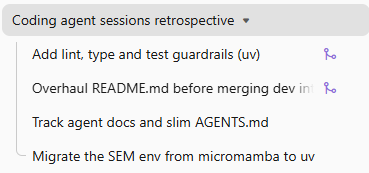
\includegraphics[height=23.4mm]{assets/screens/claude-app-forks.png}};
    \begin{scope}[shift={(shot.south west)},x={($(shot.south east)-(shot.south west)$)},
        y={($(shot.north west)-(shot.south west)$)}]
      \node[number mark] at (0.813,0.879) {1};
      \node[number mark] at (0.043,0.387) {2};
      \node[number mark] at (0.954,0.682) {3};
    \end{scope}
    \foreach \t [count=\k] in {one session,{its forks, one per task},pull request merged} {
      \node[number mark] at (56.4,-33.6-\k*6.6+6.6) {\k};
      \node[key] at (59.6,-33.6-\k*6.6+6.6) {\t};
    }
    \fill[termbg,rounded corners=1.2mm] (100,-31.4) rectangle (144,-45.6);
    \foreach \c [count=\i] in {termdot1,termdot2,termdot3} \fill[\c] (100.4+\i*2.3,-34) circle (0.7);
    \node[inner sep=0pt,font=\ttfamily\fontsize{7}{8}\selectfont,text=termdim] at (124.6,-34)
      {second terminal};
    \draw[white!18!termbg,line width=0.4pt] (100,-36.6) -- (144,-36.6);
    \node[mono,text=termfg] at (102.4,-39.6) {\textcolor{termgreen}{\$} claude -c --fork-session};
    \node[mono,text=termfg] at (102.4,-43) {> work in a worktree};
    \node[anchor=north west,inner sep=0pt,font=\scriptsize,text=udsgrey] at (100,-47.4)
      {forks the latest session in this folder};
  \end{tikzpicture}
  \note{\textbf{24:00--24:50}\par
    A tip from daily use: a session often turns into more than one task.\par
    Fork it with slash fork rather than start again: each fork keeps the whole conversation, the
      plan and the decisions included.\par
    Then ask each fork to work in a worktree; Claude Code creates one under .claude/worktrees and
      moves the session into it.\par
    Until then both forks work in the same folder, and their edits can collide.\par
    In the app the forks sit under their session in the sidebar: here four tasks that came out of
      one session, each in its own worktree; purple marks a merged pull request.\par
    In a terminal, slash fork copies the conversation into a new session and keeps you in this
      one; from a second terminal, claude with continue and fork-session copies the latest session
      of the folder.}
\end{frame}

\section[Tests first]{Tests first}
\sectionframe{06}{Tests first}
  {How does a test written before the code keep an agent on track?}
  {\faCheckDouble}

% ---------------------------------------------------------------- the loop
\begin{frame}[source={Beck (2002), Test-Driven Development: By Example}]{Test-Driven Development (TDD)}
  \begin{tikzpicture}[x=1mm,y=1mm,
      phase/.style={box,text width=28mm,minimum height=13mm,font=\footnotesize,line width=0.8pt},
      gain/.style={inner sep=0pt,font=\footnotesize,text=udsdark,align=left},
      tick/.style={inner sep=0pt,font=\footnotesize,anchor=base east}]
    \useasboundingbox (0,-1.36) rectangle (144,-55);
    \node[phase,draw=udsred,fill=redtint] (red) at (72,-8)
      {{\color{udsred}\bfseries\small RED}\\[0.4mm] write a failing test for one behaviour};
    \node[phase,draw=testgreen,fill=greentint] (green) at (96,-40)
      {{\color{testgreen}\bfseries\small GREEN}\\[0.4mm] write just enough code to pass it};
    \node[phase,draw=udsblue,fill=bluetint] (ref) at (48,-40)
      {{\color{udsblue}\bfseries\small REFACTOR}\\[0.4mm] tidy the code; every test stays green};
    \draw[flow] (red.east) to[bend left=35] (green.north);
    \draw[flow] (green.west) -- (ref.east);
    \draw[flow] (ref.north) to[bend left=35] (red.west);
    \node[lbl,align=center] at (72,-27) {one behaviour\\per cycle};
    % what each step gives us; each tick sits on its gain's first baseline (with a text width,
    % a node's base is its first line); the two gains of RED start at x = 98, clear of the arrow
    % from RED to GREEN
    \node[gain,anchor=west] (g1) at (98,-5.2) {the requirement, written first};
    \node[gain,anchor=west] (g2) at (98,-10.8) {proof that the test can fail};
    \node[gain,anchor=west,text width=20mm] (g3) at (118.4,-40) {small steps,\\easy to review};
    \node[gain,anchor=west,text width=22mm] (g4) at (8,-40) {a regression net\\for later changes};
    \foreach \g/\c in {g1/udsred,g2/udsred,g3/testgreen,g4/udsblue}
      \node[tick,text=\c] at ([xshift=-1.4mm]\g.base west) {\faCheck};
    \node[gain,anchor=base] (g5) at (74,-53.4) {tests call clear interfaces: the seams};
    \node[tick,text=udsdark] at ([xshift=-1.4mm]g5.base west) {\faCheck};
  \end{tikzpicture}
  \note{\textbf{25:00--26:00}\par
    Test-driven development in Kent Beck's formulation is a short loop.\par
    Red: write a test for one behaviour and watch it fail.\par
    Green: write just enough code to make it pass.\par
    Refactor: tidy the code while all tests stay green.\par
    Then the next behaviour.\par
    What we get: the requirement written down as a test before the code exists, proof that each
      test can fail, small steps, a regression net, and pressure towards clear interfaces, the
      seams where tests observe behaviour.}
\end{frame}

% ------------------------------------------------------- why for an agent
\begin{frame}[source={Anthropic (2026), Claude Code best practices · Mathews \& Nagappan (2024), ASE ’24}]{Why tests first help an agent}
  \begin{tikzpicture}[x=1mm,y=1mm,
      node2/.style={box,minimum height=9mm,inner sep=1.6mm},
      item/.style={anchor=base west,inner sep=0pt,font=\footnotesize,text=udsdark},
      head/.style={anchor=base west,inner sep=0pt,font=\footnotesize\bfseries}]
    \useasboundingbox (0,0) rectangle (144,-54);
    % the agent edits the code and runs the tests
    \node[node2,artifact,font=\ttfamily\footnotesize\bfseries,minimum width=20mm] (src) at (12,-8) {src/};
    \node[node2,agent,font=\footnotesize\bfseries,minimum width=26mm] (ag) at (62,-8) {\faRobot\enspace agent};
    \node[node2,artifact,draw=testgreen,fill=greentint,font=\ttfamily\footnotesize\bfseries,minimum width=20mm]
      (tst) at (114,-8) {tests/};
    \draw[flow] (ag.west) -- node[lbl,above] {edits} (src.east);
    \draw[flow] (ag.east) -- node[lbl,above] {runs} (tst.west);
    \node[anchor=south,inner sep=0pt,font=\scriptsize,text=testgreen] at ([yshift=1mm]tst.north)
      {\faLock\enspace approved and committed first};
    % pass or fail comes back: the signal
    \draw[flow,draw=testgreen,line width=0.8pt] (tst.south) to[out=-90,in=-90,looseness=0.55]
      node[pos=0.5,below,inner sep=0.8mm,font=\scriptsize\bfseries,text=testgreen] {pass or fail} (ag.south);
    % what the signal gives the agent
    \node[head,text=testgreen] at (0,-28.4) {what it gives the agent};
    \foreach \t [count=\i] in {a check it runs itself,{the intent, fixed first},one small goal per cycle,
        earlier decisions still enforced}
      \node[item] at (0,-28.4-\i*4.7) {\textcolor{testgreen}{\faCheck}\enspace\t};
    % how it gets gamed: aimed at the tests, and what catches it
    \node[head,text=udsred] (gamed) at (70,-28.4) {how it gets gamed};
    \foreach \t [count=\i] in {tests edited or skipped,expected values copied from the code,
        a mock that replaces the logic,tests fitted after the code}
      \node[item] at (70,-28.4-\i*4.7) {\textcolor{udsred}{\faTimes}\enspace\t};
    \draw[udsred,line width=0.6pt,dashed,-{Stealth[length=1.7mm,width=1.3mm]}]
      ([xshift=1.5mm]gamed.east) to[out=0,in=-90] (121,-12.6);
    \node[item,text=udsblue] at (70,-53)
      {caught by: test diffs reviewed first · you rerun every test};
  \end{tikzpicture}
  \note{\textbf{26:00--27:00}\par
    Anthropic's guidance for Claude Code puts it plainly: without a check it can run, an agent
      stops when the work looks done.\par
    A failing test turns done into a signal the agent reads and iterates on.\par
    Written first, from the spec, the test records intent instead of mirroring the
      implementation, and the suite keeps earlier decisions enforced in later sessions.\par
    The failure modes are real: agents weaken, skip or edit tests, recompute expected values the
      way the code does, or replace the logic under test with a mock, a stand-in that returns
      whatever the test expects.\par
    Hence our guardrails: read the changes to the tests first, and rerun every test yourself
      rather than trust the agent's report.\par
    A benchmark study found that giving the model the tests with the task solved more problems;
      that is evidence for code generation, not for research code.}
\end{frame}

\section[Workflow]{Skills and an end-to-end workflow}
\sectionframe{07}{Skills and an end-to-end workflow}
  {How does a request become a reviewed change?}
  {\faProjectDiagram}

% ------------------------------------------------------------ what a skill is
% a lab protocol beside a skill file, row for row: what it is called, when to use it, the steps
\begin{frame}[source={Pocock (2026), mattpocock/skills v1.3.1: tdd · agentskills.io, Specification}]{A skill: a lab protocol for the agent}
  \begin{tikzpicture}[x=1mm,y=1mm,
      head/.style={anchor=north west,inner sep=0pt,font=\small\bfseries,text=udsdark},
      prot/.style={anchor=base west,inner sep=0pt,font=\footnotesize,text=udsdark},
      code/.style={anchor=base west,inner sep=0pt,font=\ttfamily\fontsize{7.2}{8.4}\selectfont,text=udsdark},
      num/.style={circle,fill=udsblue,text=white,inner sep=0pt,minimum size=3.6mm,
        font=\fontsize{7}{7}\selectfont\bfseries},
      pair/.style={udsgreymid,line width=0.5pt,dash pattern=on 1pt off 1pt},
      key/.style={fill=white,inner xsep=0.8mm,inner ysep=0.3mm,font=\scriptsize,text=udsgrey},
      say/.style={anchor=north west,inner sep=0pt,font=\scriptsize,text=udsdark}]
    \useasboundingbox (0,0) rectangle (144,-55);
    \node[head] at (0,0) {In the lab\enspace{\mdseries\color{udsgrey}a protocol}};
    \node[head] at (76,0) {In the repository\enspace{\mdseries\color{udsgrey}a skill}};
    % the protocol: a sheet on a clipboard
    \draw[udsgreylight,fill=white,line width=0.5pt,rounded corners=1.2mm] (0,-5.6) rectangle (62,-43.6);
    \fill[udsgreymid,rounded corners=0.8mm] (24,-4.3) rectangle (38,-7.1);
    \node[prot,font=\footnotesize\bfseries] at (3,-14.6) {Sample preparation};
    \node[prot,text=udsgrey] at (3,-18.6) {Use when: a specimen goes to the SEM.};
    \foreach \t [count=\i] in {Grind.,Polish.,Etch.,Check under the light microscope.} {
      \pgfmathsetmacro\y{-29-(\i-1)*4}
      \node[num] at (4.8,\y+0.95) {\i};
      \node[prot] at (8.4,\y) {\t};
    }
    % the skill: its SKILL.md in a file window, as on the slides of section 3
    \node[anchor=north west,inner xsep=1.8mm,inner ysep=0.8mm,text height=1.9mm,text depth=0.6mm,
      font=\ttfamily\fontsize{7}{8}\selectfont,text=udsdark] (tab) at (76,-5.6)
      {\textcolor{udsblue}{\faIcon[regular]{file-alt}}\enspace tdd/SKILL.md\enspace
       \textcolor{udsgreymid}{\sffamily\scriptsize shortened}};
    \begin{scope}
      \clip[rounded corners=1.2mm] (76,-5.6) rectangle (144,-43.6);
      \fill[darktint] (tab.north east) rectangle (144,-9.7);
      \draw[udsblue,line width=0.9pt] (tab.north west) -- (tab.north east);
    \end{scope}
    \draw[udsgreylight,line width=0.5pt,rounded corners=1.2mm] (76,-5.6) rectangle (144,-43.6);
    \node[code] at (78.8,-14.6) {name: tdd};
    \node[code] at (78.8,-18.6) {description: Test-driven development. Use when};
    \node[code] at (78.8,-21.6) {\phantom{xx}the user wants to build features or fix};
    \node[code] at (78.8,-24.6) {\phantom{xx}bugs test-first, ...};
    \foreach \t [count=\i] in {Agree the seams to test.,Write one failing test.,
        Write just enough code to pass.,Repeat for the next behaviour.}
      \node[code] at (78.8,{-29-(\i-1)*4}) {\i. \t};
    % what matches what, the word on its line
    \foreach \y/\k in {-13.7/name,-17.7/when,-34.6/steps} {
      \draw[pair] (63.2,\y) -- (74.8,\y);
      \node[key] at (69,\y) {\k};
    }
    \node[say] at (0,-44.8) {written once; everyone in the lab follows it};
    \node[say] at (76,-44.8) {written once; the agent follows it when needed};
    % when a skill is worth writing, in a strip like the one of slide 5, 2 mm below the captions
    \fill[bluetint] (0,-49.6) rectangle (144,-55);
    \fill[udsblue] (0,-49.6) rectangle (1.2,-55);
    \node[anchor=west,inner sep=0pt,font=\footnotesize,text=udsdark] at (3.6,-52.3)
      {\textcolor{udsblue}{\faClipboardList}\enspace one procedure per kind of task};
    \node[anchor=west,inner sep=0pt,font=\footnotesize,text=udsdark] at (74,-52.3)
      {\textcolor{udsblue}{\faRedo}\enspace worth writing when the task recurs};
  \end{tikzpicture}
  \note{\textbf{27:10--28:10}\par
    Section 3 gave the agent facts about the repository; a skill gives it a procedure.\par
    It works like a lab protocol: a name, when to use it, and the steps, written once and
      followed by whoever does the task.\par
    A skill is the same for an agent: a Markdown file, here a shortened version of Pocock's
      test-driven development skill.\par
    Without one, we type the same instructions into every prompt, a little differently each
      time.\par
    Written once, the procedure is kept with the project, reviewed like code and improved in one
      place.\par
    Worth it for a task that recurs; a one-off task needs only a good prompt.}
\end{frame}

% ------------------------------------------------------------ inside a skill
\begin{frame}[fragile,source={Pocock (2026), mattpocock/skills v1.3.1: tdd · agentskills.io, Specification · Anthropic (2026), Claude Code docs: Skills · OpenAI (2026), Build skills}]{A skill: procedures loaded when needed}
  \begin{columns}[T,onlytextwidth]
    \begin{column}{0.57\textwidth}
\begin{codefile}[basicstyle=\ttfamily\fontsize{7}{8.4}\selectfont]{tdd/SKILL.md\enspace\textcolor{udsgreymid}{\sffamily\scriptsize shortened}}
---
name: tdd
description: Test-driven development. Use when the user
  wants to build features or fix bugs test-first,
  mentions "red-green-refactor", or wants integration
  tests.
---
# Test-Driven Development
## What a good test is
Tests verify behavior through public interfaces, not
implementation details. ...
See [tests.md](tests.md) for examples and
[mocking.md](mocking.md) for mocking guidelines.
\end{codefile}
      % where the skill folders go, under the file and flush with it
      {\scriptsize\color{udsgrey}\textcolor{udsblue}{\faFolderOpen}\enspace\fn{.claude/skills/} (Claude Code),
       \fn{.agents/skills/} (Codex)\par}
    \end{column}
    \begin{column}{0.4\textwidth}
      % one bracket per part of the file, level with its lines; y = 0 is the top of the file window
      \begin{tikzpicture}[x=1mm,y=1mm,
          what/.style={anchor=west,inner sep=0pt,font=\footnotesize,text=udsdark,align=left,text width=52mm,
            execute at begin node={\hyphenpenalty=10000\raggedright}}]
        \useasboundingbox (0,0) rectangle (57.6,-54);
        \def\first{6.6}\def\pitch{2.952}% the first line's top below the window's top, and the line pitch
        \foreach \a/\b/\t in {1/7/{\textcolor{udsblue}{\bfseries from the start}, like \fn{AGENTS.md}\\
              the name and description of every skill},
            8/11/{\textbf{when it runs}\\ \fn{/tdd}, or a task that matches},
            12/13/{\textbf{when the steps need them}\\ \fn{tests.md}, \fn{mocking.md} in the same folder}} {
          \pgfmathsetmacro\ya{-\first-(\a-1)*\pitch-0.5}
          \pgfmathsetmacro\yb{-\first-\b*\pitch+0.5}
          \draw[udsgreymid,line width=0.6pt] (0,\ya) -- (1.4,\ya) -- (1.4,\yb) -- (0,\yb);
          \node[what] at (3.6,{(\ya+\yb)/2}) {\t};
        }
      \end{tikzpicture}
    \end{column}
  \end{columns}
  \note{\textbf{28:10--29:20}\par
    Technically, a skill is a folder with a SKILL.md file and, where needed, more files beside
      it.\par
    The file starts with a name and a description, which says what the skill is for and when to
      use it.\par
    At the start of a session the agent sees only these lines, for every installed skill, about a
      hundred tokens each, just as it always sees AGENTS.md.\par
    The rest of the file loads when the skill runs: when we type its name, here /tdd, or when the
      agent finds that a task matches the description.\par
    Files beside it, here examples of good tests and rules for mocks, are read only when the
      steps call for them; this is called progressive disclosure.\par
    Committed with the code, the skill reaches everyone who works in the repository.}
\end{frame}

% ------------------------------------------------------------ the collection
\begin{frame}[source={Pocock (2026), mattpocock/skills v1.3.1: README · github.com/mattpocock/skills, 20 Oct 2026}]{Matt Pocock's skills: an end-to-end workflow}
  \begin{columns}[T,onlytextwidth]
    \begin{column}{0.56\textwidth}
      % the repository's address, which the screenshot's crop leaves out, as a link
      {\footnotesize\href{https://github.com/mattpocock/skills}{\faGithub\enspace\underline{\fn{mattpocock/skills}}}\par}
      \vskip1.6mm
      \begin{tikzpicture}
        \node[anchor=south west,inner sep=0pt,draw=udsgreylight,line width=0.4pt] (img) at (0,0)
          {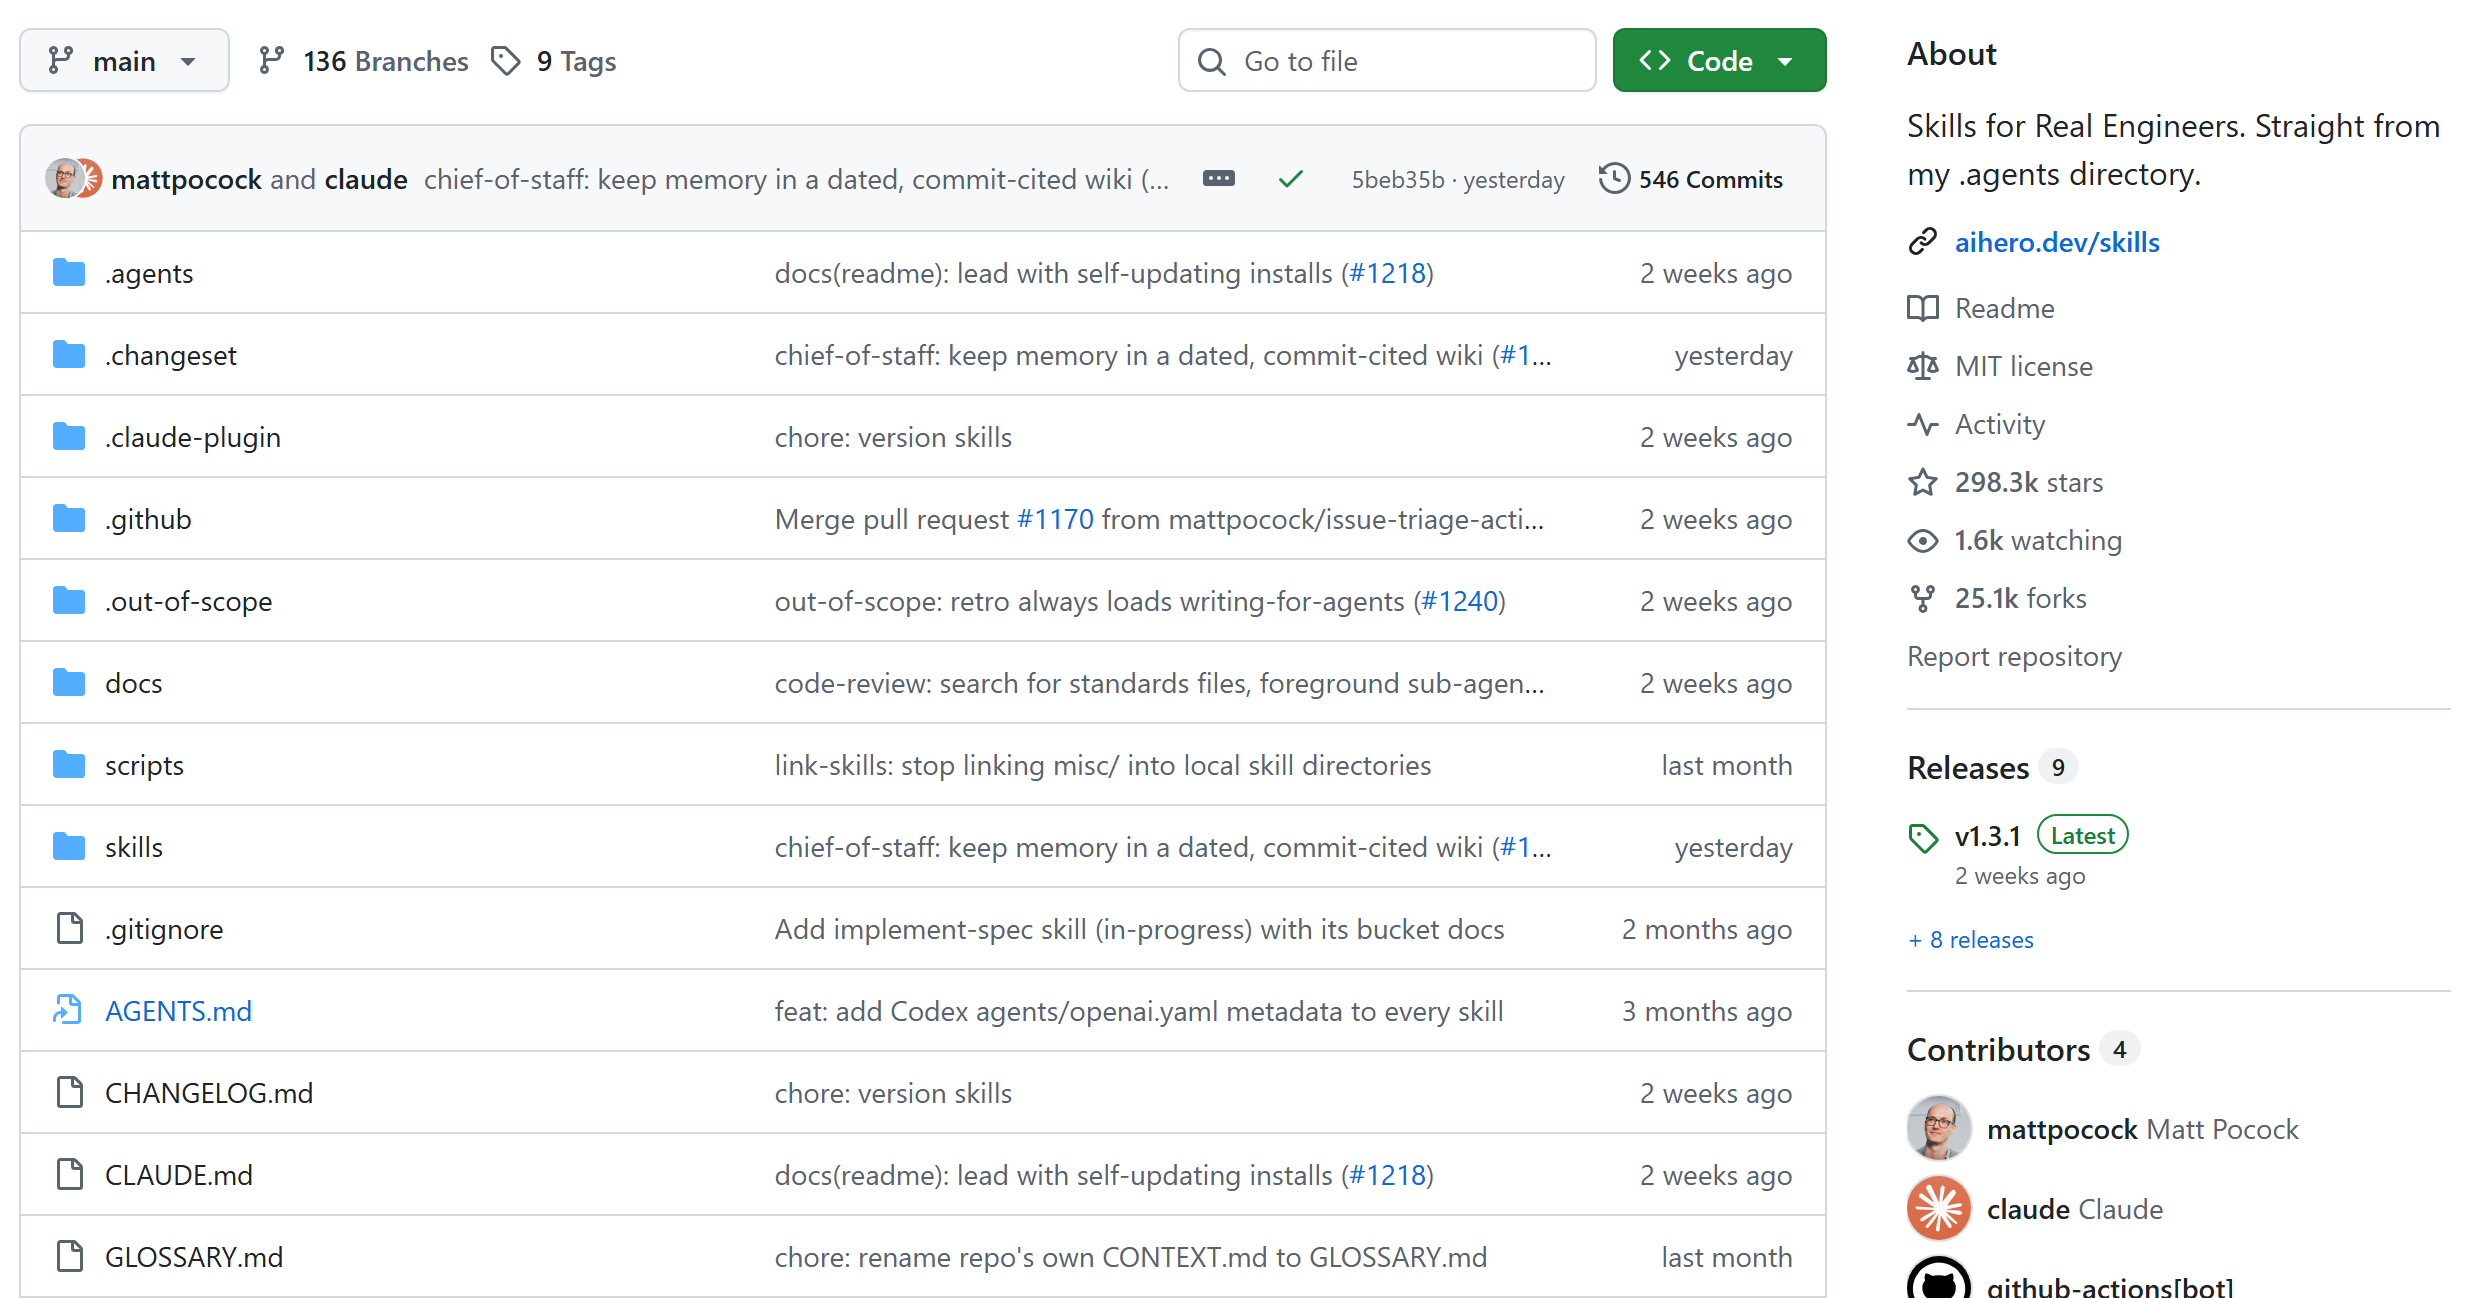
\includegraphics[width=\linewidth]{assets/screens/github-skills.png}};
        \begin{scope}[x={(img.south east)},y={(img.north west)},udsred,line width=1.1pt]
          \draw (0.014,0.320) rectangle (0.077,0.374);
          \draw (0.014,0.193) rectangle (0.109,0.247);
          \draw (0.014,0.005) rectangle (0.123,0.058);
          \draw (0.766,0.333) rectangle (0.871,0.386);
        \end{scope}
      \end{tikzpicture}
    \end{column}
    \begin{column}{0.41\textwidth}
      % two kinds of skill: the ones you type run a stage, and call the ones the agent may also pick
      \begin{tikzpicture}[x=1mm,y=1mm,
          kind/.style={anchor=north west,inner sep=0pt,font=\footnotesize\bfseries},
          chip/.style={anchor=west,minimum height=4.6mm,inner xsep=1mm,inner ysep=0pt,line width=0.5pt,
            font=\ttfamily\fontsize{7}{8}\selectfont,text=udsdark},
          you/.style={chip,draw=udsred,fill=redtint,minimum width=23.6mm},
          it/.style={chip,draw=udsblue,fill=bluetint,minimum width=22mm},
          call/.style={-{Stealth[length=1.5mm,width=1.1mm]},line width=0.5pt,draw=udsdark},
          say/.style={anchor=north west,inner sep=0pt,font=\scriptsize,text=udsgrey}]
        \useasboundingbox (0,0) rectangle (59,-54);
        \node[kind,text=udsred] at (0,0) {\faUser\enspace you type};
        \node[kind,text=udsblue] at (31,0) {\faRobot\enspace the agent may use};
        \foreach \s [count=\i from 0] in {/grill-with-docs,/to-spec,/to-tickets,/implement}
          \node[you] (u\i) at (0,{-7.6-\i*6.4}) {\s};
        \foreach \s [count=\i from 0] in {domain-modeling,codebase-design,tdd,code-review}
          \node[it] (m\i) at (31,{-7.6-\i*6.4}) {\s};
        % who calls whom, as the SKILL.md files say
        \draw[call] (u0.east) -- (m0.west);
        \draw[call] (u3.east) -- (m2.west);
        \draw[call] (u3.east) -- (m3.west);
        \draw[call] (m2.east) to[out=0,in=0,looseness=1.6] (m1.east);
        \node[say] at (0,-31.6) {each runs one stage};
        \node[say] at (31,-31.6) {rules and vocabulary};
        % installing: the files are copied into the project
        \fill[termbg,rounded corners=1mm] (0,-37) rectangle (57,-45.8);
        \foreach \c [count=\i] in {termdot1,termdot2,termdot3} \fill[\c] (\i*2.3,-39.2) circle (0.7);
        \node[inner sep=0pt,font=\ttfamily\fontsize{7}{8}\selectfont,text=termdim] at (28.5,-39.2) {install};
        \node[anchor=west,inner sep=0pt,font=\ttfamily\fontsize{7}{8}\selectfont,text=termfg] at (1.8,-43.4)
          {\textcolor{termgreen}{\$} npx skills@latest add mattpocock/skills};
        \node[say,text=udsred] at (0,-47.6) {\faExclamationTriangle\enspace read them first};
      \end{tikzpicture}
    \end{column}
  \end{columns}
  \note{\textbf{29:20--30:10}\par
    Our example is Matt Pocock's open-source collection on GitHub; the repository uses its own
      AGENTS.md and GLOSSARY.md.\par
    Its skills come in two kinds: the ones we type each run one stage of the work, and they call
      skills that the agent may also pick up by itself, which hold the rules.\par
    Grill-with-docs calls domain-modeling, implement calls tdd and code-review, and tdd looks up
      codebase-design for its vocabulary.\par
    The installer copies the files into the project; skills are instructions and scripts written
      by someone else, so read them before the agent uses them.}
\end{frame}

% ------------------------------------------------------- the books behind
% \bookcover{x}{colour}{title}{author}{year}: a book seen from the front, 22 x 27 mm, its top-left
% corner at (x,0); the darker strip on the left is the spine
\newcommand\bookcover[5]{%
  \begin{scope}
    \clip[rounded corners=0.9mm] (#1,0) rectangle ++(22,-27);
    \fill[#2] (#1,0) rectangle ++(22,-27);
    \fill[black,opacity=0.22] (#1,0) rectangle ++(1.9,-27);
  \end{scope}
  \node[anchor=north west,inner sep=0pt,text width=17.6mm,align=left,font=\scriptsize\bfseries,
    text=white,execute at begin node={\hyphenpenalty=10000\raggedright}] at (#1+3,-2.6) {#3};
  \node[anchor=south west,inner sep=0pt,text width=17.6mm,align=left,font=\scriptsize,
    text=white!80!#2] at (#1+3,-2.4-22.2) {#4\\#5};}
\begin{frame}[source={Hunt \& Thomas (1999) · Beck (1999; 2002) · Fowler (1999) · Evans (2003) · Ousterhout (2018) · Pocock (2026), mattpocock/skills v1.3.1: README, code-review, codebase-design}]{Classic practice, adapted for agents}
  % each book, the idea the skills take from it, and the skills that carry it
  \begin{tikzpicture}[x=1mm,y=1mm,
      idea/.style={anchor=north west,inner sep=0pt,text width=22mm,align=left,font=\scriptsize,
        text=udsdark,execute at begin node={\hyphenpenalty=10000\raggedright}},
      sk/.style={spec skill},
      fl/.style={spec chip}]
    \useasboundingbox (0,0) rectangle (144,-54);
    \bookcover{0}{udsdark}{The Pragmatic Programmer}{Andrew Hunt,\\David Thomas}{1999}
    \bookcover{24.4}{udsblue}{Extreme Programming Explained}{Kent Beck}{1999}
    \bookcover{48.8}{udsdark}{Refactoring}{Martin Fowler}{1999}
    \bookcover{73.2}{testgreen}{Test-Driven Development: By Example}{Kent Beck}{2002}
    \bookcover{97.6}{udsblue}{Domain-Driven Design}{Eric Evans}{2003}
    \bookcover{122}{udsdark}{A Philosophy of Software Design}{John\\Ousterhout}{2018}
    \foreach \x/\t in {0/{no one knows exactly what they want},24.4/{user stories; invest in the design every day},
        48.8/{code smells},73.2/{red, green, refactor},97.6/{a ubiquitous language},122/{deep modules}}
      \node[idea] at (\x,-29.4) {\t};
    \node[sk] at (0,-39.6) {/grill-with-docs};
    \node[sk] at (24.4,-39.6) {/to-spec};
    \node[sk] at (48.8,-39.6) {/code-review};
    \node[sk] at (73.2,-39.6) {/tdd};
    \node[fl] at (97.6,-39.6) {GLOSSARY.md};
    \node[sk] at (97.6,-45.2) {/domain-modeling};
    \node[sk] at (122,-39.6) {/codebase-design};
  \end{tikzpicture}
  \note{\textbf{30:10--31:20}\par
    None of this is new: Pocock's README says the skills rest on decades of engineering
      experience, and quotes the books.\par
    The Pragmatic Programmer: no one knows exactly what they want, so the agent asks before it
      builds; its tracer bullets return as the vertical slices of to-tickets.\par
    Kent Beck's Extreme Programming brought the user stories that to-spec writes into every spec,
      and the advice to invest in the design every day.\par
    Fowler's Refactoring catalogues code smells, which code-review looks for in every diff.\par
    Beck's red, green, refactor loop, the subject of section 6, is the tdd skill.\par
    Evans: one ubiquitous language for people and code, our glossary; Ousterhout: deep modules,
      much behaviour behind a small interface.\par
    What is new is the reader: the model has read these books, so a term such as tracer bullets
      or red and green brings the whole practice into a skill in a few words.}
\end{frame}

% Pocock's README, section "Why These Skills Exist", word for word (mattpocock/skills, MIT licence;
% the same on main on 3 November 2026 as in v1.3.1), with its links and the aside on the commit of its example glossary dropped: notes pages of their
% own, outside the frame, so they follow slide 29's notes page and stay out of the audience PDF. A
% note outside a frame does not get the theme's note style, so each one sets it first.
\note{\parindent=0pt\parskip=1.1mm\raggedright\footnotesize
  \textbf{Slide 29, continued (1 of 5): Pocock's README, ``Why These Skills Exist''}\par
  I built these skills as a way to fix common failure modes I see with Claude Code, Codex, and other
    coding agents.\par
  \textbf{\#1: The Agent Didn't Do What I Want}\par
  \emph{``No-one knows exactly what they want''}\enspace--- David Thomas \& Andrew Hunt, The Pragmatic
    Programmer\par
  \textbf{The Problem}. The most common failure mode in software development is misalignment. You think
    the dev knows what you want. Then you see what they've built - and you realize it didn't understand
    you at all.\par
  This is just the same in the AI age. There is a communication gap between you and the agent. The fix
    for this is a \textbf{grilling session} - getting the agent to ask you detailed questions about what
    you're building.\par
  \textbf{The Fix} is to use: \fn{/grill-me} - for non-code uses; \fn{/grill-with-docs} - same as
    \fn{/grill-me}, but adds more goodies (see below).\par
  These are my most popular skills. They help you align with the agent before you get started, and
    think deeply about the change you're making. Use them \emph{every} time you want to make a
    change.}
\note{\parindent=0pt\parskip=1.1mm\raggedright\footnotesize
  \textbf{Slide 29, continued (2 of 5)}\par
  \textbf{\#2: The Agent Is Way Too Verbose}\par
  \emph{``With a ubiquitous language, conversations among developers and expressions of the code are
    all derived from the same domain model.''}\enspace--- Eric Evans, Domain-Driven-Design\par
  \textbf{The Problem}: At the start of a project, devs and the people they're building the software
    for (the domain experts) are usually speaking different languages.\par
  I felt the same tension with my agents. Agents are usually dropped into a project and asked to figure
    out the jargon as they go. So they use 20 words where 1 will do.\par
  \textbf{The Fix} for this is a shared language. It's a document that helps agents decode the jargon
    used in the project.\par
  Example: here's an example glossary, from my \fn{course-video-manager} repo. Which one is easier to
    read? \textbf{BEFORE}: ``There's a problem when a lesson inside a section of a course is made `real'
    (i.e.\ given a spot in the file system)''. \textbf{AFTER}: ``There's a problem with the
    materialization cascade''. This concision pays off session after session.}
\note{\parindent=0pt\parskip=1.1mm\raggedright\footnotesize
  \textbf{Slide 29, continued (3 of 5)}\par
  \textbf{\#2, continued}\par
  This is built into \fn{/grill-with-docs}. It's a grilling session, but that helps you build a shared
    language with the AI, and document hard-to-explain decisions in ADR's.\par
  It's hard to explain how powerful this is. It might be the single coolest technique in this repo.
    Try it, and see.\par
  Tip: a shared language has many other benefits than reducing verbosity: \textbf{variables, functions
    and files are named consistently}, using the shared language; as a result, the \textbf{codebase is
    easier to navigate} for the agent; the agent also \textbf{spends fewer tokens on thinking}, because
    it has access to a more concise language.}
\note{\parindent=0pt\parskip=1.1mm\raggedright\footnotesize
  \textbf{Slide 29, continued (4 of 5)}\par
  \textbf{\#3: The Code Doesn't Work}\par
  \emph{``Always take small, deliberate steps. The rate of feedback is your speed limit. Never take on a
    task that's too big.''}\enspace--- David Thomas \& Andrew Hunt, The Pragmatic Programmer\par
  \textbf{The Problem}: Let's say that you and the agent are aligned on what to build. What happens when
    the agent \emph{still} produces crap?\par
  It's time to look at your feedback loops. Without feedback on how the code it produces actually runs,
    the agent will be flying blind.\par
  \textbf{The Fix}: You need the usual tranche of feedback loops: static types, browser access, and
    automated tests.\par
  For automated tests, a red-green-refactor loop is critical. This is where the agent writes a failing
    test first, then fixes the test. This helps give the agent a consistent level of feedback that
    results in far better code.\par
  I've built a \textbf{\fn{/tdd} skill} you can slot into any project. It encourages red-green-refactor
    and gives the agent plenty of guidance on what makes good and bad tests.\par
  For debugging, I've also built a \textbf{\fn{/diagnosing-bugs}} skill that wraps best debugging
    practices into a disciplined loop, gated phase by phase.}
\note{\parindent=0pt\parskip=1.1mm\raggedright\footnotesize
  \textbf{Slide 29, continued (5 of 5)}\par
  \textbf{\#4: We Built A Ball Of Mud}\par
  \emph{``Invest in the design of the system \emph{every day}.''}\enspace--- Kent Beck, Extreme Programming
    Explained\par
  \emph{``The best modules are deep. They allow a lot of functionality to be accessed through a simple
    interface.''}\enspace--- John Ousterhout, A Philosophy Of Software Design\par
  \textbf{The Problem}: Most apps built with agents are complex and hard to change. Because agents can
    radically speed up coding, they also accelerate software entropy. Codebases get more complex at an
    unprecedented rate.\par
  \textbf{The Fix} for this is a radical new approach to AI-powered development: caring about the design
    of the code.\par
  This is built in to every layer of these skills: \fn{/to-spec} quizzes you about which modules you're
    touching before creating a spec.\par
  And crucially, \fn{/improve-codebase-architecture} surveys a codebase for deepening opportunities and
    hands you the candidates. I recommend running it on your codebase once every few days. It is a
    survey, not a rescue: on a genuinely old codebase it will find real candidates, but it won't
    untangle the mud for you.\par
  \textbf{Summary}: Software engineering fundamentals matter more than ever. These skills are my best
    effort at condensing these fundamentals into repeatable practices, to help you ship the best apps of
    your career. Enjoy.}

% ------------------------------------------------------------ flow diagram
\begin{frame}[source={Pocock (2026), mattpocock/skills v1.3.1}]{Pocock's flow: who does what}
  \begin{tikzpicture}[x=1mm,y=1mm,
      cell/.style={minimum width=24.4mm,text width=23.2mm,inner sep=0.6mm,align=center,
        execute at begin node={\hyphenpenalty=10000}},
      hcell/.style={cell,human,minimum height=9.6mm,font=\fontsize{7}{8}\selectfont},
      acell/.style={cell,agent,minimum height=17mm,font=\fontsize{7}{8}\selectfont},
      fcell/.style={cell,artifact,minimum height=7.6mm,font=\ttfamily\fontsize{7}{8}\selectfont},
      lane/.style={font=\fontsize{7}{8}\selectfont\bfseries,rotate=90,anchor=center,inner sep=0pt}]
    \node[lane,text=udsred]  at (3,-4.8)  {PERSON};
    \node[lane,text=udsblue] at (3,-23.5) {AGENT};
    \node[lane,text=udsdark] at (3,-39)   {OUTPUT};
    \foreach \skill/\act/\who/\res [count=\k from 0] in {
        grill-with-docs/{questions in rounds; updates the glossary}/{answer; settle the open points}/{GLOSSARY.md, ADR draft},
        to-spec/{writes the spec from the conversation}/{approve scope and acceptance}/{spec (file or issue)},
        to-tickets/{vertical slices, in order}/{approve slices and order}/{ticket files},
        implement/{drives /tdd at the agreed seams; runs the review; commits}/{confirm test seams; rerun the tests}/{code + tests, one commit},
        code-review/{standards and spec, in parallel; proposes refactoring}/{judge findings; review the science}/{report (in session)}} {
      \pgfmathsetmacro\x{20+\k*27.6}
      \node[hcell] (h\k) at (\x,-4.8) {\who};
      \node[acell] (a\k) at (\x,-23.5) {{\ttfamily\bfseries/\skill}\\[0.3mm]\act};
      \node[fcell] (f\k) at (\x,-39) {\res};
      % two-way: the person both steers the stage and decides on its output
      \draw[flow,{Stealth[length=1.7mm,width=1.3mm]}-{Stealth[length=1.7mm,width=1.3mm]},draw=udsred]
        (h\k.south) -- (a\k.north);
      \draw[flow] (a\k.south) -- (f\k.north);
    }
    \foreach \k [evaluate=\k as \n using int(\k+1)] in {0,...,3} \draw[flow,draw=udsblue] (a\k.east) -- (a\n.west);
    \node[artifact,anchor=north west,minimum width=134.6mm,minimum height=5mm,font=\scriptsize,inner sep=0.6mm]
      (ctx) at (7.8,-45.4) {read along the way:\enspace \texttt{AGENTS.md}\enspace\textperiodcentered\enspace
      \texttt{GLOSSARY.md}\enspace\textperiodcentered\enspace\texttt{docs/adr/}\enspace\textperiodcentered\enspace
      \texttt{CODING\_STANDARDS.md} (review)\enspace\textperiodcentered\enspace tests};
    \foreach \a/\b/\t in {7.8/87.4/{one session: clarify, specify, slice},
                          90.6/142.4/{a fresh session per ticket}} {
      \draw[udsgreymid,line width=0.5pt] (\a,-52.5) -- ++(0,-1.2) -- (\b,-53.7) -- ++(0,1.2);
      \node[lbl,anchor=north] at ({(\a+\b)/2},-54.1) {\t};
    }
  \end{tikzpicture}
  \note{\textbf{31:20--32:30}\par
    The main flow as the author documents it: clarify with grill-with-docs, write the spec, cut
      tickets, implement each ticket.\par
    In today's terms this is spec-driven development: an approved spec before any code, then each
      ticket built test-first.\par
    Tickets are vertical slices: each a thin path through the whole program, from the command
      line to the output, usable on its own.\par
    Implement drives the tdd skill at the test seams agreed in the spec, the public functions
      and command-line options that the tests call; then it runs code-review and commits.\par
    Code-review checks the repository's coding standards and the spec, and is where refactoring
      is proposed.\par
    Red marks the decisions that stay with us at every stage.\par
    The author's context advice: one session from clarification to tickets, then a fresh session
      per ticket that starts from the written ticket.}
\end{frame}

% ---------------------------------------------------- a grilling session
% \sessiondot{n}: the theme's \numbermark, 3.6 mm across; \sessionmark{n} is the same without height, so a
% marker on a session line does not move the lines around it
\newcommand\sessiondot[1]{\tikz[baseline=-0.75ex]\node[circle,fill=udsred,text=white,inner sep=0pt,
  minimum size=3.6mm,font=\sffamily\fontsize{7}{7}\selectfont\bfseries] {#1};}
\newcommand\sessionmark[1]{\smash{\sessiondot{#1}}}
% \sessionarrow{text}: a session line, then an arrow from its end across the column gap to the
% window in the right column; drawn inside the frame, so the notes thumbnail shows it too. The
% terminal's text sits 3.2 mm inside its right edge (1 mm box separation plus 2.2 mm padding).
\newcommand\sessionarrow[1]{%
  \setbox0\hbox{\setbox2\hbox{x}\spaceskip=\wd2 #1}\copy0
  \edef\sessionarrowend{\the\dimexpr\linewidth+3.2mm+\colgap-\wd0+0.1mm\relax}%
  \tikz[overlay,baseline=0pt]\draw[udsred,line width=0.8pt,-{Stealth[length=2mm,width=1.6mm]}]
    (1.4mm,0.9mm) -- (\sessionarrowend,0.9mm);}
\begin{frame}[fragile,source={Pocock (2026), mattpocock/skills v1.3.1: grill-with-docs, grilling, domain-modeling}]{A \texttt{/grill-with-docs} session}
  % the gap between the columns, which the glossary arrow crosses
  \edef\colgap{\the\dimexpr0.03\textwidth\relax}
  \begin{columns}[T,onlytextwidth]
    \begin{column}{0.61\textwidth}
\begin{terminal}[basicstyle=\ttfamily\fontsize{7}{8}\selectfont]{example session}
> /grill-with-docs Add validation folds by specimen to the
  training CLI, as decided in ADR-0003.
§\textcolor{termred}{\smash{\faQuestionCircle}}§ §\textbf{Q1 Default number of folds}§: the manifest lists §\sessionmark{1}§
  three specimens. One fold per specimen?
§\textcolor{termblue}{\smash{\faArrowRight}}§ Yes: k = number of specimens; --folds can lower it. §\sessionmark{2}§

§\textcolor{termred}{\smash{\faQuestionCircle}}§ §\textbf{Q2 What validation claims}§: each specimen is the only
  one of its material state, a term GLOSSARY.md lacks.
  Report folds as unseen material states, and add it?
§\textcolor{termblue}{\smash{\faArrowRight}}§ Yes.

§\textcolor{termred}{\smash{\faQuestionCircle}}§ §\textbf{Q3 Rows without specimen\_id}§: stop with a ValueError,
  as CODING_STANDARDS.md asks?
§\textcolor{termblue}{\smash{\faArrowRight}}§ Yes, and name the rows in the message.
> yes to all
§\sessionarrow{Updated GLOSSARY.md: Material state.}§
No ADR: the number of folds is easy to change later. §\sessionmark{3}§
\end{terminal}
    \end{column}
    \begin{column}{0.36\textwidth}
      % the legend on top; the glossary window at the bottom, level with the line that updates it
      \begin{minipage}[t][58mm][t]{\linewidth}
        \footnotesize
        \begin{tabular}{@{}c@{\enspace}l@{}}
          \sessiondot{1} & a fact the agent looked up\\[1.4mm]
          \sessiondot{2} & a recommended answer\\[1.4mm]
          \sessiondot{3} & an ADR only if hard to reverse\\
        \end{tabular}
        \vfill
\begin{codefile}[basicstyle=\ttfamily\fontsize{7}{8}\selectfont]{GLOSSARY.md\enspace\textcolor{udsgreymid}{new entry}}
Material state: the processing
  condition of a specimen (AsCast,
  Q980_0h_WC, Q980_9h_AC); here,
  one specimen per state.
\end{codefile}
        \vspace{-2.2mm}% the box's own skip below it, so its bottom meets the terminal's
      \end{minipage}
    \end{column}
  \end{columns}
  \note{\textbf{32:30--33:50}\par
    What grilling looks like on our request; the session is abridged and written for our example
      in the format of Pocock's skills.\par
    Each round asks every question that can be asked now, numbered, each with a recommended
      answer (2), worded so that yes accepts it.\par
    The agent looks up facts itself, here the number of specimens in the manifest (1), and
      leaves the decisions to us.\par
    When a term settles, it goes into the glossary at once (the arrow); here the session finds
      that every specimen is also the only one of its material state, which matters for what
      validation can claim.\par
    It offers an ADR only when a decision is hard to reverse, surprising and a real trade-off,
      so the number of folds gets none (3).\par
    Pocock's video of July 2026 shows a full session on his own project.}
\end{frame}

% ------------------------------------------------------------- walkthrough
% \stagefile{node}{x centre}{y top}{tab}{body}: a small file window under a stage, drawn as the
% codefile box is; (node) is its page and (nodet) its tab
\newcommand\stagefile[5]{%
  \node[anchor=north west,inner xsep=1mm,inner ysep=0.7mm,text height=1.9mm,text depth=0.5mm,
    font=\ttfamily\fontsize{7}{8}\selectfont,text=udsdark] (#1t) at (#2-12.2,#3)
    {\textcolor{udsblue}{\faIcon[regular]{file-alt}}\enspace#4};
  \node[anchor=north,minimum width=24.4mm,text width=22mm,inner xsep=1.2mm,inner ysep=1.3mm,
    align=left,font=\ttfamily\fontsize{7}{8.4}\selectfont,text=udsdark] (#1) at (#2,#3-4.2) {#5};
  \begin{scope}
    \clip[rounded corners=1mm] (#2-12.2,#3) rectangle ($(#1.south)+(12.2,0)$);
    \fill[darktint] (#1t.north east) rectangle (#2+12.2,#3-4.2);
    \draw[udsblue,line width=1.4pt] (#1t.north west) -- (#1t.north east);
  \end{scope}
  \draw[udsgreylight,line width=0.5pt,rounded corners=1mm] (#2-12.2,#3) rectangle ($(#1.south)+(12.2,0)$);}
\begin{frame}{The specimen split, stage by stage}
  \begin{tikzpicture}[x=1mm,y=1mm,
      stage/.style={agent,minimum width=24.4mm,minimum height=6.2mm,inner sep=0.6mm,
        font=\ttfamily\bfseries\fontsize{7}{8}\selectfont},
      ticket/.style={draw=udsgreylight,fill=white,line width=0.5pt,anchor=north,minimum width=24.4mm,
        text width=21.4mm,inner xsep=1.5mm,inner ysep=0.9mm,align=left,font=\scriptsize,text=udsdark,
        execute at begin node={\hyphenpenalty=10000\raggedright},
        path picture={\fill[udsdark] (path picture bounding box.north west) rectangle
          ([xshift=0.9mm]path picture bounding box.south west);}},
      say/.style={anchor=north,inner sep=0pt,font=\scriptsize,text=udsgrey,align=center,text width=25mm,
        execute at begin node={\hyphenpenalty=10000}},
      commit/.style={circle,draw=udsblue,fill=white,line width=0.9pt,minimum size=3mm,inner sep=0pt}]
    % an invisible copy of a lane label of "Pocock's flow: who does what" gives this picture the
    % same left edge, so the five columns sit exactly under those of that slide
    \node[font=\fontsize{7}{8}\selectfont\bfseries,rotate=90,anchor=center,inner sep=0pt,opacity=0]
      at (3,-4.8) {PERSON};
    % the short request starts the flow
    \fill[termbg,rounded corners=1mm] (7.8,0) rectangle (142.6,-6.4);
    \foreach \c [count=\i] in {termdot1,termdot2,termdot3} \fill[\c] (7.8+\i*2.3,-3.2) circle (0.7);
    \node[anchor=west,inner sep=0pt,font=\ttfamily\fontsize{7}{8}\selectfont,text=termfg] at (17,-3.2)
      {> Add validation folds by specimen to the training CLI, as decided in ADR-0003.};
    % the five stages, as on "Pocock's flow: who does what"
    \foreach \s [count=\k from 0] in {grill-with-docs,to-spec,to-tickets,implement,code-review}
      \node[stage] (s\k) at (20+\k*27.6,-13.6) {/\s};
    \draw[flow] (20,-6.4) -- (s0.north);
    \foreach \k [evaluate=\k as \n using int(\k+1)] in {0,...,3} \draw[flow,draw=udsblue] (s\k.east) -- (s\n.west);
    \foreach \k in {0,...,4} \draw[flow] (s\k.south) -- ++(0,-3.4);
    % 1: answers, and a new glossary term
    \stagefile{w0}{20}{-21.2}{GLOSSARY.md}{\textcolor{testgreen}{+}\,Material state}
    \node[say] at ([yshift=-1.4mm]w0.south) {Q1 to Q3 answered};
    % 2: the spec
    \stagefile{w1}{47.6}{-21.2}{spec.md}{\textcolor{udsblue}{\bfseries\#\# Decisions}\\
      \textcolor{udsblue}{\bfseries\#\# Test seams}\\ \textcolor{udsblue}{\bfseries\#\# Out of scope}}
    % 3: three vertical slices, each usable on its own
    \node[ticket] (t1) at (75.2,-21.2) {\textbf{T1}\enspace\fn{--split specimen}, end to end};
    \node[ticket] (t2) at ([yshift=-1.4mm]t1.south) {\textbf{T2}\enspace overlap guard and errors};
    \node[ticket] (t3) at ([yshift=-1.4mm]t2.south) {\textbf{T3}\enspace provenance in the fold file};
    % 4: one commit per ticket, each in a fresh session
    \draw[udsblue,line width=1pt] (95.4,-20.4) -- (95.4,-45.6);
    \foreach \t [count=\i from 0] in {T1,T2,T3} {
      \node[commit] (k\i) at (95.4,-24-\i*8.6) {};
      \node[anchor=west,inner sep=0pt,font=\scriptsize,text=udsdark] at ([xshift=1.4mm]k\i.east)
        {\textbf{\t}\enspace tests, code};
    }
    \node[say] at (102.8,-47.6) {a fresh session per ticket};
    % 5: the review report on two axes
    \stagefile{w4}{130.4}{-21.2}{report}{\fontsize{7}{8.4}\sffamily
      \textcolor{udsblue}{\faSearch}\enspace standards\\[0.4mm] \textcolor{udsblue}{\faSearch}\enspace spec}
    \node[say] at ([yshift=-1.4mm]w4.south) {findings for you to judge};
  \end{tikzpicture}
  \note{\textbf{33:50--35:00}\par
    The whole flow on our task, starting from the short request.\par
    Each stage leaves something we can open and check.\par
    Grilling settles what the repository leaves open: the default number of folds, and what
      validation is meant to show with only three specimens.\par
    The spec records the decisions and the test seams.\par
    Tickets are thin vertical slices, each usable on its own: first the whole path from the
      command line to a fold file, then the overlap guard and the error cases, then the
      provenance stored in the fold file.\par
    Each ticket is implemented test-first in a fresh session, and review checks the standards
      and the spec.}
\end{frame}

% ------------------------------------------------- /implement drives /tdd
\begin{frame}[source={Pocock (2026), mattpocock/skills v1.3.1: implement, tdd · aihero.dev/skills}]{How \texttt{/implement} uses \texttt{/tdd}}
  \begin{columns}[T,onlytextwidth]
    \begin{column}{0.48\textwidth}
      \begin{tikzpicture}[x=1mm,y=1mm,
          stp/.style={agent,text width=48mm,minimum height=6.6mm,align=left,font=\scriptsize,inner sep=1mm},
          num/.style={font=\scriptsize\bfseries,text=udsblue,anchor=east,inner sep=0.8mm}]
        \node[anchor=north west,inner sep=0pt,font=\footnotesize] at (0,0)
          {\fn{/implement}: one ticket, one fresh session};
        \node[stp,anchor=north west] (s1) at (6,-5)  {read the ticket};
        \node[stp,anchor=north west,draw=testgreen,fill=greentint,line width=0.8pt,minimum height=9mm] (s2) at (6,-14)
          {\fn{/tdd} at the agreed seams: one failing test, then just enough code to pass it};
        \node[stp,anchor=north west] (s3) at (6,-26) {typecheck; run single test files};
        \node[stp,anchor=north west] (s4) at (6,-35) {run the full suite once};
        \node[stp,anchor=north west] (s5) at (6,-44) {\fn{/code-review}, then commit};
        \foreach \i in {1,...,5} \node[num] at (s\i.west) {\i};
        \foreach \i [evaluate=\i as \j using int(\i+1)] in {1,...,4} \draw[flow] (s\i.south) -- (s\j.north);
        \draw[flow,draw=testgreen] ([yshift=-2.2mm]s2.east) -- ++(3.5,0) -- ++(0,4.4)
          node[midway,right,lbl,text=testgreen] {repeat} -- ++(-3.5,0);
      \end{tikzpicture}
    \end{column}
    \begin{column}{0.49\textwidth}
      \begin{gblock}[fontupper=\footnotesize]{Rules of the \texttt{/tdd} loop}
        \begin{itemize}\setlength\itemsep{0.5mm}
          \item seams agreed with you first
          \item one failing test, then minimal code
          \item one vertical slice per cycle
          \item tests only through public interfaces
          \item mocks only at system boundaries
          \item refactoring left to \fn{/code-review}
        \end{itemize}
      \end{gblock}
      {\footnotesize Known gaps: code written before its test; ticket left open; the run reviews its own
       work.\par}
    \end{column}
  \end{columns}
  \note{\textbf{35:00--36:10}\par
    In Pocock's skills, implement is the build step and you invoke it yourself, one ticket per
      fresh session.\par
    It reads the ticket, drives the tdd skill at the agreed seams one red-green slice at a time,
      typechecks and runs single test files as it goes, runs the full suite once at the end,
      calls code-review and commits.\par
    The tdd skill is a set of rules: seams agreed first, red before green, one vertical slice
      per cycle, tests through public interfaces, mocks only at system boundaries.\par
    The loop has no refactor step, because agents almost never do it; code-review
      proposes refactoring instead.\par
    The author's documentation lists the gaps: the agent sometimes writes code first, implement
      does not close the ticket, and the review inside the same run reviews its own work, so a
      fresh session makes a better reviewer.}
\end{frame}

% ---------------------------------------------------- when is it worth it
\begin{frame}[source={Pocock (2026), mattpocock/skills v1.3.1, ask-matt}]{When is the full flow worth it?}
  \centering
  \begin{tikzpicture}[x=1.55mm,y=1mm,pt/.style={circle,fill=udsdark,inner sep=0pt,minimum size=1.8mm}]
    \fill[bluetint] (0,0) rectangle (42,23);
    \fill[redtint] (42,23) rectangle (84,46);
    \draw[udsgreylight,line width=0.4pt] (42,0) -- (42,46) (0,23) -- (84,23);
    \draw[flow] (0,0) -- (86,0);
    \draw[flow] (0,0) -- (0,48);
    \node[lbl,anchor=north east,text=udsdark,font=\footnotesize] at (86,-0.8) {changes what a result means};
    \node[lbl,anchor=south,rotate=90,text=udsdark,font=\footnotesize] at (-0.8,24) {size and open questions};
    \node[lbl,anchor=south west,text=udsblue,font=\footnotesize\bfseries] at (1,1) {one prompt, review the diff};
    \node[lbl,anchor=north east,text=udsred,font=\footnotesize\bfseries] at (83,45) {grill, spec, tickets};
    \node[lbl,anchor=north west,text=udsdark,font=\footnotesize\bfseries] at (1,45) {slice it into tickets};
    \node[lbl,anchor=south east,text=udsdark,font=\footnotesize\bfseries] at (83,1) {write a short spec};
    \foreach \x/\y/\t in {7/9/fix a plot label, 14/16/add a CLI flag, 5/35/refactor the data loader,
        50/11/pixel-size units, 50/29/change the split unit, 60/38/new loss or metric} {
      \node[pt] (p) at (\x,\y) {};
      \node[lbl,anchor=west,text=udsdark,font=\scriptsize] at (p.east) {\t};
    }
  \end{tikzpicture}
  \note{\textbf{36:10--36:50}\par
    Not every change needs five stages.\par
    Two questions decide: how large or open is the change, and does it change what a result
      means?\par
    Small changes that leave results unchanged go straight to the agent; we still read the
      diff.\par
    A small change of meaning, such as pixel-size units, deserves a short spec.\par
    A large routine refactor benefits from tickets.\par
    The full flow earns its overhead when both hold, as for a new split unit, loss or
      metric.\par
    Pocock's own routing asks whether the build spans several sessions; the axis of meaning is
      ours.}
\end{frame}

\section[Adoption]{A realistic starting point}
\sectionframe{08}{A realistic starting point}
  {What should I change in my repository first?}
  {\faSeedling}

% ---------------------------------------------------- other skill packages
% \pkgcard{k}{owner}{repository}{head colour}{author}{what it is}{its steps}{its rule for tests}: card k
% (0 to 2), 46 mm wide and 3 mm apart; the green box at its foot holds the rule, level with the other
% cards' rules
\newcommand\pkgcard[8]{%
  \pgfmathsetmacro\pkx{#1*49}%
  \begin{scope}
    \clip[rounded corners=1.2mm] (\pkx,0) rectangle ++(46,-45.4);
    \fill[white] (\pkx,0) rectangle ++(46,-45.4);
    \fill[#4] (\pkx,0) rectangle ++(46,-9.2);
    \fill[greentint] (\pkx,-32.6) rectangle ++(46,-12.8);
    \fill[testgreen] (\pkx,-32.6) rectangle ++(1.2,-12.8);
  \end{scope}
  \draw[udsgreylight,line width=0.5pt,rounded corners=1.2mm] (\pkx,0) rectangle ++(46,-45.4);
  \node[anchor=north west,inner sep=0pt,font=\ttfamily\fontsize{7}{8.4}\selectfont,text=white!70!#4,
    align=left] at (\pkx+1.8,-1.5) {#2/\\\textcolor{white}{\bfseries #3}};
  \node[pkg who] at (\pkx+1.8,-10.8) {#5};
  \node[pkg what] at (\pkx+1.8,-14.8) {#6};
  \node[pkg text] at (\pkx+1.8,-22.6) {#7};
  \node[pkg text,text width=40.6mm] at (\pkx+3.6,-34.4) {\textcolor{testgreen}{\faCheck}\enspace #8};}
\begin{frame}[source={GitHub, 3 Nov 2026: obra/superpowers v7.0.1 · multica-ai/andrej-karpathy-skills · mattpocock/skills v1.3.1}]{Other skill packages}
  \begin{tikzpicture}[x=1mm,y=1mm,
      pkg who/.style={anchor=north west,inner sep=0pt,font=\scriptsize,text=udsgrey,text width=42.4mm,align=left},
      pkg what/.style={anchor=north west,inner sep=0pt,font=\footnotesize\bfseries,text=udsdark,
        text width=42.4mm,align=left,execute at begin node={\hyphenpenalty=10000\raggedright}},
      pkg text/.style={anchor=north west,inner sep=0pt,font=\scriptsize,text=udsdark,text width=42.4mm,
        align=left,execute at begin node={\hyphenpenalty=10000\raggedright}}]
    \useasboundingbox (0,0) rectangle (144,-54);
    \pkgcard{0}{mattpocock}{skills}{udsdark}{Matt Pocock}{small skills you combine}
      {grill, spec, tickets, implement, review}{\fn{/tdd}: red before green, at agreed seams}
    \pkgcard{1}{obra}{superpowers}{udsblue}{Jesse Vincent}{a whole method in 15 skills}
      {brainstorm, plan, execute, review, finish}{no production code without a failing test first}
    \pkgcard{2}{multica-ai}{andrej-karpathy-skills}{udsblue}{from Karpathy's notes}{one \fn{CLAUDE.md}, four rules}
      {think first, keep it simple, change only what is asked, set checkable goals}
      {a bug fix starts with a test that reproduces the bug}
    % what all three share
    \fill[greentint] (0,-48) rectangle (144,-54);
    \node[anchor=west,inner sep=0pt,font=\footnotesize\bfseries,text=testgreen] at (2,-51)
      {\faCheckDouble\enspace in all three, the check is set before the code is written};
  \end{tikzpicture}
  \note{\textbf{37:00--38:00}\par
    Pocock's collection is one of several; two others are worth a look.\par
    Superpowers, by Jesse Vincent, is a whole method, from brainstorming to finishing the
      branch; its test-driven skill allows no production code without a failing test.\par
    The Karpathy skills are one CLAUDE.md with four rules, written by Jiayuan Zhang from Andrej
      Karpathy's notes on how models go wrong in code; the last rule turns a task into a goal
      that can be checked, such as a test that reproduces a bug.\par
    They differ in how much of the process they take over; Pocock's README prefers small skills
      you combine to systems that own the process.\par
    What they share is section 6: the check is decided before the code.\par
    As with any skill, read them before installing.}
\end{frame}

% --------------------------------------------------------------- checklist
\begin{frame}{Checklist for your repository}
  \setbeamertemplate{itemize item}{\raisebox{-0.1ex}{\textcolor{udsblue}{\faSquare[regular]}}}
  \setlength\leftmargini{5mm}
  \begin{columns}[T,onlytextwidth]
    \begin{column}{0.3\textwidth}
      \textbf{\color{udsdark}Groundwork}\par\vskip1mm
      \begin{itemize}\footnotesize\setlength\itemsep{2mm}
        \item a git repository; commit before each agent task
        \item the Python environment (conda, uv, etc.)
        \item Ruff and mypy configured, run after every edit
      \end{itemize}
    \end{column}
    \begin{column}{0.31\textwidth}
      \textbf{\color{udsblue}Context}\par\vskip1mm
      \begin{itemize}\footnotesize\setlength\itemsep{2mm}
        \item \fn{AGENTS.md}: commands, boundaries, pointers
        \item \fn{GLOSSARY.md}: the key terms
        \item \fn{CODING\_STANDARDS.md}: what review checks
        \item \fn{docs/adr/}: decisions people reopen
      \end{itemize}
    \end{column}
    \begin{column}{0.33\textwidth}
      \textbf{\color{udsred}Workflow}\par\vskip1mm
      \begin{itemize}\footnotesize\setlength\itemsep{2mm}
        \item a workflow that suits you, e.g.\
          \href{https://github.com/mattpocock/skills}{\faGithub\enspace\underline{\fn{mattpocock/skills}}}
        \item your own skills for the tasks you repeat
        \item tests agreed before the code
        \item one worktree, or a forked session, per task
        \item you review the code and the science
      \end{itemize}
    \end{column}
  \end{columns}
  \note{\textbf{38:00--38:50}\par
    Groundwork: a git repository with a commit before every agent task, the Python environment
      with conda or uv, and Ruff and mypy run after every edit.\par
    Context: AGENTS.md, the glossary, the coding standards and ADRs, so that requests can stay
      short.\par
    Workflow: choose one that suits you, Pocock's skills for example; write your own skills for
      the tasks you repeat; agree the tests before the code; give each task its own worktree or
      forked session; and review the code and the science yourself.\par
    None of this needs a new tool, and most of it helps human collaborators too.}
\end{frame}

% --------------------------------------------------------------- thank you
% the title slide's layout: its blue panel on the right, the thanks where the title was; drawn
% inside the frame, so that the notes' thumbnail shows it too
\begin{frame}[plain,noframenumbering]
\vbox to 0pt{\vskip-2mm\hbox to 0pt{\hskip-8mm\begin{tikzpicture}[x=1mm,y=1mm]
  \useasboundingbox (0,0) rectangle (160,-90);
  \titlepanel
  \node[anchor=north west,inner sep=0pt] at (8,-8) {\includegraphics[width=30mm]{\udslogo}};
  \node[anchor=north west,inner sep=0pt,text width=88mm,align=left] at (8,-36) {%
    {\fontsize{32}{36}\selectfont\bfseries\color{udsblue}Thank you\par}\vskip4mm
    \textcolor{udsred}{\rule{14mm}{0.8pt}}\par\vskip3mm
    {\fontsize{11}{13}\selectfont\color{udsdark}\insertauthor\par}};
\end{tikzpicture}\hss}\vss}
\par\rule{0pt}{80mm}
\note{\textbf{38:50--39:20}\par
    Thank you.\par
    Questions to open the discussion: which of your projects is not under git yet; which
      repository you would try this on first, and who reviews it; which decision in your project deserves an
      ADR; which single command tells you that your code still works.\par
    Templates, tool details and references follow in the appendix.}
\end{frame}

\appendix
% the footer numbers appendix slides A1, A2, ..., as their titles do
\setcounter{framenumber}{0}
\renewcommand\insertframenumber{A\arabic{framenumber}}
% Appendix: its own sections, so the mini-frame headline shows only these.
\section[Templates]{Templates}

% ------------------------------------------------------------- AGENTS.md
\begin{frame}[fragile]{A1\enspace Template: \texttt{AGENTS.md}}
  \begin{columns}[T,onlytextwidth]
    \begin{column}{0.62\textwidth}
\begin{codefile}[basicstyle=\ttfamily\fontsize{7}{8.4}\selectfont]{AGENTS.md}
# <project>: notes for coding agents
## Setup and checks
- Environment: `<create and activate command>`
- Fast check (CPU, synthetic data, under a minute): `<command>`
- Lint and types: `<command>`
## Where things are
- Vocabulary: `GLOSSARY.md`; decisions: `docs/adr/`
## Conventions the code does not show
- <units, coordinate frames, file formats, splitting rules>
## Boundaries
- Read-only: `data/raw/`, <other protected paths>
- Ask before: new dependencies, deleting files, cluster jobs
- Never: commit secrets or data; push to `main`
- Never edit a test just to make it pass
## When you finish
- Changed files, commands run, assumptions, open questions
\end{codefile}
    \end{column}
    \begin{column}{0.35\textwidth}
      \footnotesize
      \begin{itemize}\setlength\itemsep{1.4mm}
        \item each line prevents a mistake you have seen
        \item point to documents; do not copy them
        \item update it in the commit that makes it stale
        \item Codex: nested files per sub-package; an override replaces one folder's file
        \item other tools read other names, e.g.\ \fn{CLAUDE.md}
      \end{itemize}
    \end{column}
  \end{columns}
\end{frame}

% --------------------------------------- glossary, coding standards, ADR
\begin{frame}[fragile,source={Nygard (2011) · Pocock (2026), domain-modeling ADR format; code-review}]{A2\enspace Templates: glossary, coding standards and ADR}
  \begin{columns}[T,onlytextwidth]
    \begin{column}{0.48\textwidth}
\begin{codefile}[basicstyle=\ttfamily\fontsize{7}{8.4}\selectfont]{GLOSSARY.md}
# Glossary
<Term>: one-sentence definition (`code_name`).
  Relates to: <other terms and how>.
  Avoid: <synonyms we do not use>.
<Term>: ...
\end{codefile}
      \vskip2mm
\begin{codefile}[basicstyle=\ttfamily\fontsize{7}{8.4}\selectfont]{CODING\_STANDARDS.md}
# Coding standards
- Randomness: <how seeds are passed>
- Errors: <what public functions raise>
- Tests: <fixtures, seams, expected values>
- <a judgement call a reviewer can check>
\end{codefile}
    \end{column}
    \begin{column}{0.49\textwidth}
\begin{codefile}[basicstyle=\ttfamily\fontsize{7}{8.4}\selectfont]{docs/adr/NNNN-short-title.md}
# ADR-NNNN: <short noun phrase>
Status: proposed | accepted |
        superseded by ADR-NNNN
## Context
Forces at play: data, constraints, question.
## Decision
What we will do, in full sentences.
## Considered options
Alternatives and why they lost.
## Consequences
What follows, including the costs.
\end{codefile}
    \end{column}
  \end{columns}
\end{frame}


\section[Tool details]{Tool details}

% --------------------------------------------------------------------- uv
% A3 and A4 are kept for questions after slide 6; their notes say so instead of giving a time
\begin{frame}[fragile,source={Astral (2026), uv documentation: projects, running commands, lockfile; uv README and its speed benchmark}]{A3\enspace The upgrade: uv}
  \begin{columns}[T,onlytextwidth]
    \begin{column}{0.49\textwidth}
      {\footnotesize\bfseries A uv project\par}\vskip1.2mm
      \begin{foldertree}[note at=29.5]
        \tdir{0}{sem-seg/}{all committed except \fn{.venv/}}
        \tfile{1}{pyproject.toml}{what the project needs}
        \tfile{1}{uv.lock}{exact versions, every platform}
        \tfile{1}{.python-version}{the Python version}
        \tdir{1}{.venv/}{rebuilt from \fn{uv.lock}}
      \end{foldertree}
      \footnotesize
      \begin{itemize}\setlength\itemsep{1.2mm}
        \item one tool instead of pip, venv, pip-tools, pipx and pyenv
        \item much faster than pip
        \item \fn{uv run}: nothing to activate; the environment is synced first
      \end{itemize}
    \end{column}
    \begin{column}{0.48\textwidth}
\begin{terminal}[basicstyle=\ttfamily\fontsize{7}{8.6}\selectfont]{terminal}
$ uv init sem-seg            # new project
$ uv python pin 3.12         # .python-version
$ uv add numpy pandas torch  # updates uv.lock
$ uv add --dev pytest ruff mypy
$ uv run pytest -q           # sync, then run
$ uv sync                    # rebuild .venv
\end{terminal}
    \end{column}
  \end{columns}
  \note{\textbf{If asked}\par
    uv, from Astral, the makers of Ruff, is one tool for what pip, venv, pip-tools, pipx and
      pyenv do separately.\par
    A project is a pyproject.toml with what the project needs and a uv.lock with the exact
      version of every package for every platform; commit both.\par
    uv builds the environment in .venv inside the project; it is not committed and can be
      rebuilt at any time.\par
    uv add adds a package and updates the lockfile; tools for development, such as pytest, Ruff
      and mypy, go into their own group.\par
    uv run checks that lockfile and environment are in sync and then runs the command, so there
      is nothing to activate, which suits an agent whose commands each start a fresh shell.\par
    Astral reports 10 to 100 times the speed of pip.\par
    The current version is 0.13; uv has not reached 1.0, but Astral treats it as stable.}
\end{frame}

% ------------------------------------------------------------ conda or uv
\begin{frame}[source={conda (2026) · Astral (2026), uv: PyTorch integration · prefix.dev (2026), pixi}]{A4\enspace conda or uv?}
  % one question decides; the rest of the comparison is what slide 6 and A3 show
  \begin{tikzpicture}[x=1mm,y=1mm,
      ask/.style={human,text width=60mm,inner sep=1.6mm,font=\footnotesize,align=center},
      tool/.style={agent,anchor=north,text width=58mm,inner sep=1.8mm,font=\footnotesize,align=left},
      yn/.style={lbl,font=\scriptsize\bfseries}]
    \def\fact{\ttfamily\fontsize{7}{8.4}\selectfont}
    \node[ask] (q) at (72,-4.6) {\textbf{needs non-Python packages?}\\[0.3mm]
      \scriptsize CUDA toolkits, GDAL, compilers};
    \node[tool] (c) at (34,-17) {{\color{udsblue}\bfseries conda}\enspace from conda-forge, or pixi\\[1mm]
      \fact environment.yml + lockfile\\ conda run -n sem-seg \dots};
    \node[tool] (u) at (110,-17) {{\color{udsblue}\bfseries uv}\enspace Python packages from PyPI\\[1mm]
      \fact pyproject.toml + uv.lock\\ uv run \dots};
    \draw[flow] (q.west) -| node[yn,pos=0.75,left] {yes} (c.north);
    \draw[flow] (q.east) -| node[yn,pos=0.75,right] {no} (u.north);
    % the one extra step for GPU work with uv
    \node[ask,anchor=north,text width=50mm] (g) at (110,-35.4) {\textbf{GPU PyTorch on Windows?}};
    \draw[flow] (u.south) -- (g.north);
    \node[agent,anchor=north,text width=50mm,inner sep=1.6mm,font=\footnotesize,align=center] (i) at (110,-45.2)
      {PyTorch's index in \fn{pyproject.toml}\\ \scriptsize PyPI's Windows wheels are CPU-only};
    \draw[flow] (g.south) -- node[yn,right] {yes} (i.north);
    % common ground
    \node[anchor=north west,inner sep=0pt,font=\scriptsize,text=udsdark,text width=64mm,align=left] at (2,-35.6)
      {\textbf{either way}\\ one project file defines the environment\\ exact versions in a lockfile\\
       one command runs the code\\ about five commands to learn};
  \end{tikzpicture}
  \note{\textbf{If asked}\par
    One question decides: does the project need packages that are not Python?\par
    conda installs packages of any language from conda-forge, including CUDA toolkits, GDAL or
      compilers; uv installs Python packages from PyPI and nothing else.\par
    Both can now pin exact versions: uv with its lockfile, conda with its own lockfile since
      version 26.5 or with conda-lock.\par
    conda keeps environments in a central folder, uv in the project.\par
    For GPU work, conda-forge has CUDA builds, while PyPI's PyTorch wheels for Windows are
      CPU-only, so a uv project needs PyTorch's own index in its pyproject.toml, as the uv guide
      shows.\par
    The learning curve is small: a handful of commands, and the habit that the project file, not
      the shell, defines the environment.\par
    If a project needs non-Python packages, stay with conda, or look at pixi, which installs
      conda-forge packages with a lockfile and uses uv for PyPI packages.}
\end{frame}

% ------------------------------------------------------- Codex discovery
\begin{frame}[source={OpenAI (2026), Custom instructions with AGENTS.md · Codex configuration reference}]
  {A5\enspace Codex: how instruction files are found}
  \begin{tikzpicture}[x=1mm,y=1mm,
      file/.style={artifact,minimum width=33mm,minimum height=5.2mm,inner sep=0.6mm,font=\ttfamily\scriptsize},
      dir/.style={box,minimum width=40mm,minimum height=5.2mm,inner sep=0.6mm,font=\ttfamily\scriptsize}]
    % ---- left: one folder
    \node[anchor=north west,inner sep=0pt,font=\small\bfseries] at (0,0) {Within one folder: replacement};
    \node[file,anchor=north west] (o1) at (2,-6.5) {AGENTS.override.md};
    \node[file,anchor=north west] (o2) at (2,-14)  {AGENTS.md};
    \node[file,anchor=north west] (o3) at (2,-21.5){fallback names};
    \foreach \a/\b in {o1/o2,o2/o3} \draw[flow] (\a.south) -- (\b.north);
    \draw[udsgreymid,line width=0.5pt] ([xshift=2mm]o1.north east) -- ++(1.2,0) |- ([xshift=2mm]o3.south east);
    \node[anchor=west,text width=28mm,align=left,font=\scriptsize,inner sep=0pt,
      execute at begin node={\hyphenpenalty=10000}] at ([xshift=4.5mm]o2.east)
      {checked top to bottom; the first non-empty file is used};
    \node[anchor=north west,text width=64mm,font=\footnotesize,inner sep=0pt] at (0,-31)
      {At most \textbf{one file per folder}: an override \emph{replaces} the \fn{AGENTS.md} beside it.};
    \draw[udsgreylight,line width=0.4pt] (69,0) -- (69,-41);
    % ---- right: chain of folders
    \node[anchor=north west,inner sep=0pt,font=\small\bfseries] at (73,0) {Across folders: layering};
    \foreach \t [count=\i from 0] in
        {\textasciitilde/.codex/\ (global),repository root (.git),src/,src/sem\_seg/,src/sem\_seg/data/\ \ <- cwd} {
      \node[dir,anchor=north west] (d\i) at (74,-6-\i*6.7) {\t};
    }
    \draw[udsred,line width=0.9pt] (d4.north west) rectangle (d4.south east);
    \foreach \i [evaluate=\i as \j using int(\i+1)] in {0,...,3} \draw[flow] (d\i.south) -- (d\j.north);
    \draw[udsblue,line width=0.6pt,-{Stealth[length=1.7mm]}] (119,-6.5) -- (119,-37.3);
    \node[anchor=west,text width=22.5mm,align=left,font=\scriptsize,inner sep=0pt] at (120.5,-22)
      {concatenated top to bottom; later files take \textbf{precedence}};
    \node[anchor=north west,font=\footnotesize,inner sep=0pt] at (73,-40.5)
      {Folders below or beside \texttt{cwd}: \textbf{not} loaded.};
    % ---- caveats
    \foreach \t [count=\i from 0] in
      {{Built \textbf{once per run}: restart Codex after editing an instruction file.},
       {\fn{project\_doc\_max\_bytes} (default 32\,KiB) limits instruction \emph{text}; it is not the model's context window.},
       {Check what loaded: ask Codex to summarize its current instructions.}} {
      \node[box,fill=darktint,draw=none,anchor=north west,text width=43mm,align=left,
        font=\scriptsize,minimum height=9.5mm] at (\i*49,-44.5) {\t};
    }
  \end{tikzpicture}
\end{frame}


% ------------------------------------------------- Pocock: video vs current
\begin{frame}[source={Pocock (2026), video of 16 Jul 2026 · mattpocock/skills v1.3.1 · aihero.dev/skills}]{A6\enspace Pocock's workflow, then and now}
  \scriptsize\renewcommand\arraystretch{1.28}\setlength\tabcolsep{3pt}
  \begin{tabularx}{\textwidth}{@{}>{\bfseries}L{22mm}L{55mm}X@{}}
    \toprule
    & \bfseries Video (16 July 2026, between v1.1 and v1.2) & \bfseries Documentation, v1.3.1 (October 2026)\\
    \midrule
    Domain file  & \fn{CONTEXT.md} plus ADRs & \fn{GLOSSARY.md} plus ADRs; the skills read only \fn{GLOSSARY.md}\\
    Main flow    & \fn{/grill-with-docs}, then \fn{/implement} directly, or \fn{/to-spec}, \fn{/to-tickets},
                   \fn{/implement} (which runs \fn{/code-review}) &
                   \fn{/grill-with-docs}, \fn{/to-spec}, \fn{/to-tickets}, \fn{/implement} (which drives \fn{/tdd}
                   and runs \fn{/code-review}); \fn{/implement-spec} for a whole spec\\
    Grilling     & one question at a time & numbered rounds, each question with a recommended answer\\
    Local tickets& one \fn{tickets.md} & one file per ticket under \fn{.scratch/<feature>/issues/}\\
    Context      & ``smart zone'' of about 140k tokens (heuristic); clear before each ticket &
                   about 150k tokens (heuristic); one session for clarifying to ticketing, a fresh one per ticket\\
    Testing      & not shown & \fn{/tdd}: red to green at agreed seams; refactoring moved to \fn{/code-review}\\
    Installation & \fn{npx skills@latest add mattpocock/skills} & Claude Code plugin recommended; \fn{npx} for other agents\\
    \bottomrule
  \end{tabularx}
\end{frame}

\section[Sources]{Sources}

% -------------------------------------------------------------- references
\begin{frame}{A7\enspace References: tools and workflow}
  \scriptsize\setlength\parskip{0.9mm}\vskip-\parskip
  OpenAI (2026). \emph{Custom instructions with AGENTS.md}.
  \url{https://learn.chatgpt.com/docs/agent-configuration/agents-md}, accessed 19~Oct~2026.\par
  OpenAI (2026). Codex documentation: \emph{Configuration reference}, \emph{Agent approvals and security},
  \emph{Non-interactive mode}, \emph{Build skills}. \url{https://learn.chatgpt.com/docs}, accessed 19--22~Oct~2026.\par
  AGENTS.md: a simple, open format for guiding coding agents. \url{https://agents.md/}, accessed 19~Oct~2026.\par
  Agent Skills format. \url{https://agentskills.io/}, accessed 19~Oct~2026.\par
  Anthropic (2026). Claude Code documentation: \emph{Best practices}, \emph{Memory}, \emph{Checkpointing}, \emph{Tools
  reference}, \emph{Worktrees}, \emph{Desktop}, \emph{CLI reference}, \emph{Sessions}.
  \url{https://code.claude.com/docs}, accessed 20~Oct~2026, \emph{Sessions} 4~Nov~2026.\par
  Anthropic (2026). \emph{Prompting Claude Opus 5.5}.
  \url{https://platform.claude.com/docs/en/build-with-claude/prompt-engineering/prompting-claude-opus-5-5};
  OpenAI (2026). \emph{Using GPT-6}. \url{https://developers.openai.com/api/docs/guides/latest-model};
  both accessed 4~Nov~2026.\par
  M.~Pocock (2026). \emph{mattpocock/skills}, v1.3.1, commit 49dd158 (9~Oct~2026), MIT licence.
  \url{https://github.com/mattpocock/skills}\par
  M.~Pocock (2026). \emph{AI skills for real engineers}, \url{https://www.aihero.dev/skills}, and \emph{v1.3: /implement-spec,
  /pr, /retro, and GLOSSARY.md}, 5~Oct~2026,
  \url{https://www.aihero.dev/skills-changelog-v13-implement-spec-pr-retro-and-glossary-md}\par
  M.~Pocock (2026). \emph{mattpocock/skills: A complete AI coding workflow, end-to-end}. YouTube, 16~Jul~2026.
  \url{https://www.youtube.com/watch?v=M6mYodf0dJM}\par
\end{frame}

\begin{frame}{A8\enspace References: git, environments and checks}
  \scriptsize\setlength\parskip{0.9mm}\vskip-\parskip
  S.~Chacon, B.~Straub (2014). \emph{Pro Git}, 2nd ed. Apress. \url{https://git-scm.com/book}; git documentation,
  \emph{git-worktree}, \url{https://git-scm.com/docs/git-worktree}, accessed 20--21~Oct~2026.\par
  Layout of the worktree diagram, accessed 21~Oct~2026: Anthropic Academy (2026), figure of worktree branches
  merged into main, \url{https://academy.claude.com/assets/media/536e6bef11940caea62b1d41d10070eb1e2a220811cb0ff388da1af20b4d2c79.png};
  DevToolLab (2026), worktrees guide, \url{https://devtoollab.com/blog/claude-code-git-worktrees-parallel-agents-guide}.\par
  conda (2026). Documentation, v26.9: \emph{Managing environments}, \emph{conda run}, \emph{New features}.
  \url{https://docs.conda.io}, accessed 20~Oct~2026.\par
  Anaconda (2025). \emph{Terms of service}, 15~Jul~2025; \emph{Academic policy}, 14~Jul~2025.
  \url{https://www.anaconda.com/legal/terms/terms-of-service}\par
  conda-forge (2026). \emph{Miniforge}. \url{https://github.com/conda-forge/miniforge}; prefix.dev (2026). \emph{pixi
  documentation}, v0.82. \url{https://pixi.prefix.dev}\par
  Astral (2026). \emph{uv documentation}, v0.13: projects, running commands, PyTorch integration.
  \url{https://docs.astral.sh/uv/}, accessed 20~Oct~2026; README with its speed benchmark, \url{https://github.com/astral-sh/uv}.\par
  Astral (2026). \emph{Ruff documentation}, v0.17: rules, configuration, editor setup.
  \url{https://docs.astral.sh/ruff/}\par
  mypy documentation, v2.4. \url{https://mypy.readthedocs.io}; Microsoft (2026). \emph{Pylance} README and FAQ,
  \url{https://github.com/microsoft/pylance-release}; \emph{Mypy Type Checker}, \url{https://github.com/microsoft/vscode-mypy};
  VS Code documentation: \emph{Source control}, \emph{Python environments}, \emph{Editing Python},
  \url{https://code.visualstudio.com/docs}, accessed 20~Oct~2026.\par
\end{frame}

\begin{frame}{A9\enspace References: methods and evidence}
  \scriptsize\setlength\parskip{0.9mm}\vskip-\parskip
  K.~Beck (2002). \emph{Test-Driven Development: By Example}. Addison-Wesley.\par
  M.~Nygard (2011). \emph{Documenting architecture decisions}. Cognitect blog, 15~Nov~2011.
  \url{https://www.cognitect.com/blog/2011/11/15/documenting-architecture-decisions}\par
  DrivenData (2026). \emph{Cookiecutter Data Science}, v2: a project layout for data science.
  \url{https://cookiecutter-data-science.drivendata.org/}, accessed 4~Nov~2026.\par
  N.~S.~Mathews, M.~Nagappan (2024). \emph{Test-driven development for code generation}. ASE~’24.
  \url{https://doi.org/10.1145/3691620.3695527}; arXiv:2402.13521\par
  S.~Kapoor, A.~Narayanan (2023). \emph{Leakage and the reproducibility crisis in machine-learning-based science}.
  Patterns 4(9), 100804. \url{https://doi.org/10.1016/j.patter.2023.100804}\par
  B.-I.~Bachmann, M.~Stiefel, M.~Müller, F.~T.~Mücklich (2026). \emph{A systematically designed open-access SEM
  dataset and robustness benchmark for machine learning-based microstructure segmentation: a high-chromium cast iron
  case study}. Zenodo, v1, CC~BY~4.0. \url{https://doi.org/10.5281/zenodo.21931379}; DFG project MU~959/57-1.\par
\end{frame}

\begin{frame}{A10\enspace References: books and skill packages}
  \scriptsize\setlength\parskip{0.9mm}\vskip-\parskip
  A.~Hunt, D.~Thomas (1999). \emph{The Pragmatic Programmer: From Journeyman to Master}. Addison-Wesley;
  20th anniversary ed., D.~Thomas, A.~Hunt (2019), \emph{The Pragmatic Programmer: Your Journey to Mastery}.\par
  K.~Beck (1999). \emph{Extreme Programming Explained: Embrace Change}. Addison-Wesley; 2nd ed.\ with C.~Andres,
  2004.\par
  M.~Fowler (1999). \emph{Refactoring: Improving the Design of Existing Code}. Addison-Wesley; 2nd ed.\ 2018.
  Chapter~3: bad smells in code.\par
  E.~Evans (2003). \emph{Domain-Driven Design: Tackling Complexity in the Heart of Software}. Addison-Wesley.\par
  J.~Ousterhout (2018). \emph{A Philosophy of Software Design}. Yaknyam Press; 2nd ed.\ 2021.\par
  Agent Skills (2026). \emph{Specification}. \url{https://agentskills.io/specification}; Anthropic (2026). Claude Code
  documentation: \emph{Skills}. \url{https://code.claude.com/docs/en/skills}, both accessed 3~Nov~2026.\par
  J.~Vincent, Prime Radiant (2026). \emph{obra/superpowers}, v7.0.1 (21~Oct~2026), MIT licence.
  \url{https://github.com/obra/superpowers}\par
  J.~Zhang (2026). \emph{andrej-karpathy-skills}, a \fn{CLAUDE.md} derived from A.~Karpathy's observations on LLM coding
  pitfalls. \url{https://github.com/multica-ai/andrej-karpathy-skills}, accessed 3~Nov~2026.\par
\end{frame}

\end{document}
.
\providecommand\notesmode{hide notes}
\setbeameroption{\notesmode}

\begin{document}
% \titlepanel: the right of the title slide, which the closing slide repeats: a blue panel with a
% request typed at a prompt and, above it, the editor where the agent changes the code: one line
% removed (red), two added (green), the second still being written at a sparkle; a red edge on its
% left. Inside a full-page tikzpicture[x=1mm,y=1mm] whose origin is the page's top-left corner,
% y downwards negative; the panel bleeds 1 mm past the edges.
\newcommand\titlepanel{%
  \coordinate (pnw) at (102,0);
  \fill[udsblue] (102,1) rectangle (161,-91);
  % centred in the blue right of the red stripe
  \begin{scope}[shift={(pnw)},xshift=0.8mm]
    \fill[udsdark] (6,-15) rectangle (52,-60);
    \fill[udsdark!70!black] (6,-15) rectangle (52,-19.5);
    \foreach \i in {0,1,2} \fill[white!55!udsdark] (9+2.6*\i,-17.25) circle (0.65);
    % the agent's edit: rows 3 (removed) and 4 and 5 (added), marked in the gutter
    \fill[udsred!55!udsdark] (6,-31.4) rectangle (52,-34.6);
    \fill[testgreen!60!udsdark] (6,-34.6) rectangle (52,-41);
    \foreach \y/\m in {-33/$-$,-36.2/+,-39.4/+}
      \node[text=white,font=\footnotesize\bfseries,inner sep=0pt] at (9.5,\y) {\m};
    % code lines: row, indent level, segment widths; the first segment of a line is brighter
    \foreach \row/\ind/\segs in {0/0/{8,15},1/1/{5,3,12},2/1/{4,14},3/1/{6,17},4/1/{6,9,8},
        5/2/{8,7},6/2/{5,10},7/1/{11,6},8/1/{7,8},10/0/{9,5,11}} {
      \pgfmathsetmacro\y{-22.8-3.2*\row}
      \pgfmathsetmacro\x{13+3.5*\ind}
      \xdef\xs{\x}
      \foreach \w [count=\k] in \segs {
        \pgfmathsetmacro\mix{\k==1 ? 85 : 50}
        \fill[white!\mix!udsdark] (\xs,\y) rectangle ++(\w,-1.2);
        \pgfmathsetmacro\nx{\xs+\w+1.4}
        \xdef\xs{\nx}
      }
    }
    % the sparkle pair right of the line being written (row 5 ends at x = 36.4, row 4 at 42.3)
    \foreach \sx/\sy/\sr in {45.6/-39.2/2.5,47.6/-37.3/1.1}
      \fill[white,shift={(\sx,\sy)},scale=\sr] (0,1) .. controls (0,0.28) and (0.28,0) .. (1,0)
        .. controls (0.28,0) and (0,-0.28) .. (0,-1) .. controls (0,-0.28) and (-0.28,0) .. (-1,0)
        .. controls (-0.28,0) and (0,0.28) .. cycle;
    % the prompt: a chevron and three words, the first word in line with the code
    \draw[white,line width=0.9pt,rounded corners=3.5mm] (6,-64.5) rectangle (52,-71.5);
    \draw[udsred!45!white,line width=1.2pt] (8.9,-66.6) -- (10.5,-68) -- (8.9,-69.4);
    \foreach \x/\w in {13/9,23.4/4,28.8/12} \fill[white!85!udsblue] (\x,-67.4) rectangle ++(\w,-1.2);
  \end{scope}
  \fill[udsred] (102,1) rectangle (103.6,-91);}

% ------------------------------------------------------------------ title
\begin{frame}[plain,noframenumbering]
% Drawn inside the frame rather than over the page, so the speaker notes' thumbnail shows it too.
% The picture's origin is the page's top-left corner: a plain frame's body starts 8 mm in and
% 2 mm down.
\vbox to 0pt{\vskip-2mm\hbox to 0pt{\hskip-8mm\begin{tikzpicture}[x=1mm,y=1mm]
  \useasboundingbox (0,0) rectangle (160,-90);
  \titlepanel
  \node[anchor=north west,inner sep=0pt] at (8,-8) {\includegraphics[width=30mm]{\udslogo}};
  \node[anchor=north west,inner sep=0pt,text width=88mm,align=left] at (8,-36) {%
    {\fontsize{25}{29}\selectfont\bfseries\color{udsblue}\inserttitle\par}\vskip2mm
    {\fontsize{15}{18}\selectfont\color{udsdark}\insertsubtitle\par}\vskip4mm
    \textcolor{udsred}{\rule{14mm}{0.8pt}}\par\vskip3mm
    {\fontsize{11}{13}\selectfont\color{udsdark}\insertauthor\par}};
  \node[anchor=south west,inner sep=0pt] (d3m) at (8,-83) {
\includegraphics[width=10mm]{assets/d3m.png}};
  \node[anchor=west,inner sep=0pt,text width=74mm,align=left,font=\fontsize{7}{8.8}\selectfont,
    execute at begin node={\hyphenpenalty=10000}] at ([xshift=3mm]d3m.east) {%
    {\color{udsblue}\insertinstitute\par}
    {\color{udsgrey}\insertdate\par}};
\end{tikzpicture}\hss}\vss}
% a frame with no tall content drops out of the notes' thumbnail; this invisible strut keeps it
\par\rule{0pt}{80mm}
\note{\textbf{0:00--0:20}\par
    Practical talk: how we prepare a repository for coding agents, how we hand over a task, and
      how we check the result.}
\end{frame}

% ---------------------------------------------------------------- outline
\begin{frame}{Outline}
  % each section's title as on its divider, and the divider's question, shortened to one line
  \small\renewcommand\arraystretch{1.32}\setlength\tabcolsep{4pt}
  \begin{tabularx}{\textwidth}{@{}>{\leavevmode\color{udsblue}\bfseries}p{4mm}>{\bfseries}p{61mm}X@{}}
    \toprule
    1 & From asking questions to delegating work & What must we provide, and what must we verify?\\
    2 & Environments and code checks             & Where does our code run, and what checks it?\\
    3 & Preparing the repository                 & What can the repository tell the agent?\\
    4 & Architecture Decision Records (ADRs)     & Why does the project work this way?\\
    5 & Version control with git                 & How do we keep and review every change?\\
    6 & Tests first                              & How do tests keep an agent on track?\\
    7 & Skills and an end-to-end workflow        & How does a request become a reviewed change?\\
    8 & A realistic starting point               & What should I change in my repository first?\\
    \bottomrule
  \end{tabularx}
  \note{\textbf{0:20--1:00}\par
    One running task carries the talk: splitting a segmentation dataset by specimen.\par
    The eight sections answer eight practical questions.\par
    Sections 2 and 5 are the groundwork that an agent needs in any project: an environment with
      automatic checks, and version control.\par
    A thread runs from the first section to the fourth: the better the repository is prepared,
      the shorter the request can be.\par
    The repository and its code are illustrative; the micrographs come from our HCCI SEM
      dataset.\par
    Claude Code, Codex and Matt Pocock's skills are the documented examples; the research-code
      examples are ours.\par
    Tool behaviour changes quickly; the appendix lists versions and access dates.}
\end{frame}

\section[Delegation]{From asking questions to delegating work}
\sectionframe{01}{From asking questions to delegating work}
  {What must we provide, and what must we verify, before an agent takes over a task?}
  {\faRobot}

% ---------------------------------------------------------- chat vs agent
\begin{frame}{From a chat assistant to a coding agent}
  \begin{tikzpicture}[x=1mm,y=1mm,
      who/.style={minimum width=15mm,minimum height=9.5mm,font=\small\bfseries}]
    % conversational assistant
    \node[anchor=north west,inner sep=0pt,font=\small\bfseries] at (0,0) {Conversational assistant};
    \node[anchor=north west,lbl,inner sep=0pt,font=\footnotesize] at (0,-4.6) {answers questions about what you paste};
    \node[human,who] (you1) at (8,-25.25) {You};
    \node[agent,who] (llm) at (56,-25.25) {Model};
    \draw[flow] ([yshift=2.2mm]you1.east) -- node[lbl,above]{question, pasted code} ([yshift=2.2mm]llm.west);
    \draw[flow] ([yshift=-2.2mm]llm.west) -- node[lbl,below]{answer, snippet} ([yshift=-2.2mm]you1.east);
    \node[anchor=north west,text width=64mm,font=\footnotesize,inner sep=0pt] at (0,-46)
      {you run the code; it sees only what you paste};
    \draw[udsgreylight,line width=0.4pt] (67,0) -- (67,-51);
    % coding agent
    \node[anchor=north west,inner sep=0pt,font=\small\bfseries] at (72,0) {Coding agent};
    \node[anchor=north west,lbl,inner sep=0pt,font=\footnotesize] at (72,-4.6) {acts in your repository};
    \node[human,who] (you2) at (79.5,-25.25) {You};
    \draw[udsblue,dashed,line width=0.5pt] (101,-10) rectangle (143.4,-40.5);
    \node[anchor=south east,lbl,text=udsblue] at (143.4,-9.8) {sandbox: repository, shell, approvals};
    \coordinate (c) at (122.2,-25.25);
    \foreach \a/\t in {90/read files,0/edit,270/run tests,180/inspect} {
      \node[agent,inner sep=1mm,font=\footnotesize] (n\a) at ($(c)+(\a:12.5 and 9.6)$) {\t};
    }
    \draw[flow,draw=udsblue] (n90.east) to[bend left=30] (n0.north);
    \draw[flow,draw=udsblue] (n0.south) to[bend left=30] (n270.east);
    \draw[flow,draw=udsblue] (n270.west) to[bend left=30] (n180.south);
    \draw[flow,draw=udsblue] (n180.north) to[bend left=30] (n90.west);
    \draw[flow] ([yshift=2.2mm]you2.east) -- node[lbl,above]{task} ([yshift=2.2mm]you2.east -| 101,0);
    \draw[flow] ([yshift=-2.2mm]you2.east -| 101,0) -- node[lbl,below]{diff, report} ([yshift=-2.2mm]you2.east);
    \node[anchor=north west,text width=71mm,font=\footnotesize,inner sep=0pt] at (72,-46)
      {loops until done; you set limits, accept or reject};
  \end{tikzpicture}
  \note{\textbf{1:10--2:20}\par
    A chat assistant answers questions; we stay the integrator and carry code and results back
      and forth.\par
    An agent has tools: it reads the repository, edits files, runs commands and iterates until
      it judges the task done.\par
    That makes delegation possible, but it works with whatever context and permissions we give
      it.\par
    Those permissions are its sandbox: the folders it may change, the commands it may run, and
      what it must ask us first.\par
    Its typical failure is not a syntax error but a reasonable-looking change that violates
      something only we know, such as how the data must be split.}
\end{frame}

% -------------------------------------------------------- running example
\begin{frame}{Running example: split the data by specimen}
  % oblique view: a point (p,q) of a micrograph lying flat goes to (p + \obs q, \obk q)
  \def\obs{0.5}\def\obk{0.42}
  \def\ow{34}\def\oh{24.51}% overview micrographs, 1000 x 721 px
  \def\dw{28}\def\dh{20.02}% detail micrographs, 1000 x 715 px
  \begin{tikzpicture}[x=1mm,y=1mm,
      sheet/.style={draw=udsdark,line width=0.35pt},
      tag/.style={anchor=south west,fill=udsdark,fill opacity=0.8,text opacity=1,text=white,
        font=\ttfamily\fontsize{7}{8}\selectfont,inner xsep=0.8mm,inner ysep=0.4mm},
      zoom/.style={udsblue,line width=0.4pt},
      side/.style={anchor=west,font=\scriptsize,inner sep=0pt}]
    % ---------------------------------------------------------------- specimens
    \node[anchor=north west,inner sep=0pt,font=\footnotesize] at (0,0) {\textbf{Specimens}\enspace one per state};
    \foreach \n [count=\i] in {AsCast,Q980\_0h\_WC,Q980\_9h\_AC} {
      \begin{scope}[shift={(18,{-10-(\i-1)*11})}]
        \fill[udsgreylight] (0,0) rectangle (12,-2);
        \fill[udsgreymid] (12,0) -- (16,3.36) -- (16,1.36) -- (12,-2) -- cycle;
        \fill[udsgreypale] (0,0) -- (12,0) -- (16,3.36) -- (4,3.36) -- cycle;
      \end{scope}
      \node[anchor=east,inner sep=0pt,font=\ttfamily\fontsize{7}{8}\selectfont] at (16.5,{-9.2-(\i-1)*11}) {\n};
      \node[anchor=east,inner sep=0pt,font=\scriptsize,text=udsgrey] at (16.5,{-12.4-(\i-1)*11}) {fold \i};
    }
    % the specimen of the running example; a tiny copy of its overview micrograph marks the imaged
    % spot (not to scale)
    \draw[udsblue,line width=0.8pt] (18,-21) -- (30,-21) -- (34,-17.64) -- (22,-17.64) -- cycle;
    \begin{scope}[cm={1,0,\obs,\obk,(18,-21)}]
      \node[anchor=south west,inner sep=0pt,transform shape] at (4.3,2.78)
        {
\includegraphics[width=3.4mm,height=2.45mm]{assets/hcci/overview-bse}};
      \draw[udsblue,line width=0.6pt] (4.3,2.78) rectangle (7.7,5.23);
      \coordinate (sa) at (7.7,5.23); \coordinate (sb) at (4.3,2.78);
    \end{scope}
    % ------------------------------------------------------------ overview area
    \node[anchor=north west,inner sep=0pt,font=\footnotesize,align=left] at (38,-10)
      {\textbf{Overview area}\\[0.3mm]{\scriptsize\color{udsgrey}66 micrographs on one pixel grid}};
    \draw[zoom] (sa) -- (38+\obs*\oh,-30+\obk*\oh) (sb) -- (38,-30);
    \foreach \img/\y in {overview-inlens/-32.8,overview-se/-31.4,overview-bse/-30} {
      \begin{scope}[cm={1,0,\obs,\obk,(38,\y)}]
        \node[anchor=south west,inner sep=0pt,transform shape] at (0,0)
          {\includegraphics[width=\ow mm,height=\oh mm]{assets/hcci/\img}};
        \draw[sheet] (0,0) rectangle (\ow,\oh);
      \end{scope}
    }
    % the detail area inside it, where the dataset README places it (section 7)
    \begin{scope}[cm={1,0,\obs,\obk,(38,-30)}]
      \draw[udsblue,line width=0.8pt] (0.6071*\ow,0.4589*\oh) rectangle (0.7999*\ow,0.6500*\oh);
      \coordinate (f1) at (0.6071*\ow,0.4589*\oh); \coordinate (f2) at (0.7999*\ow,0.4589*\oh);
      \coordinate (f3) at (0.7999*\ow,0.6500*\oh);
    \end{scope}
    % -------------------------------------------------------------- detail area
    \node[anchor=north west,inner sep=0pt,font=\footnotesize,align=left] at (89,0)
      {\textbf{Detail area}\enspace inside it, 5$\times$ finer\\[0.3mm]{\scriptsize\color{udsgrey}60 micrographs on one pixel grid}};
    % from the box's lower-left, lower-right and upper-right corners to the near corner of each
    % micrograph, so no line crosses the box
    \draw[zoom] (f1) -- (89,-40) (f2) -- (89,-32.8) (f3) -- (89,-25.6);
    % more micrographs under the stack: other microscopes, voltages and dwell times
    \foreach \y in {-42.8,-41.4} {
      \begin{scope}[cm={1,0,\obs,\obk,(89,\y)}]
        \filldraw[fill=udsgreypale,sheet] (0,0) rectangle (\dw,\dh);
      \end{scope}
    }
    % the patch: the same pixels in every micrograph of the area
    \def\pa{0.42*\dw}\def\pb{0.67*\dw}\def\pc{0.25*\dh}\def\pd{0.58*\dh}
    \foreach \img/\y/\col/\detector/\role in {detail-bse/-40/udsblue/BSE/training,
        detail-se/-32.8/udsred/SE/validation,detail-inlens/-25.6/udsblue/InLens/training} {
      \begin{scope}[cm={1,0,\obs,\obk,(89,\y)}]
        \node[anchor=south west,inner sep=0pt,transform shape] at (0,0)
          {\includegraphics[width=\dw mm,height=\dh mm]{assets/hcci/\img}};
        \draw[sheet] (0,0) rectangle (\dw,\dh);
        \fill[\col,fill opacity=0.35] (\pa,\pc) rectangle (\pb,\pd);
        \draw[\col,line width=0.9pt] (\pa,\pc) rectangle (\pb,\pd);
      \end{scope}
      \node[tag] at (89.5,\y+0.5) {\detector};
      \node[side,text=\col] at (129,\y+4) {\role};
      % the column up to the next sheet, which hides the part beneath it
      \foreach \p/\q in {\pa/\pc,\pb/\pc,\pa/\pd,\pb/\pd}
        \draw[udsdark,line width=0.35pt,dash pattern=on 0.8pt off 0.6pt]
          (89+\p+\obs*\q,\y+\obk*\q) -- ++(0,7.2);
    }
    \begin{scope}[cm={1,0,\obs,\obk,(89,-18.4)}]
      \node[anchor=south west,inner sep=0pt,transform shape] at (0,0)
        {
\includegraphics[width=\dw mm,height=\dh mm]{assets/hcci/detail-mask}};
      \draw[sheet] (0,0) rectangle (\dw,\dh);
      \draw[udsdark,line width=0.9pt] (\pa,\pc) rectangle (\pb,\pd);
    \end{scope}
    \node[side,text=udsdark] at (129,-14.4) {one mask};
    % ------------------------------------------------------------------- result
    \node[anchor=north west,inner sep=0pt,font=\footnotesize,text=udsred] at (38,-44.5)
      {\textbf{Random patch split}\enspace one area, one mask on both sides: data leakage};
    \node[anchor=north west,inner sep=0pt,font=\footnotesize] at (0,-50.5)
      {\textbf{Task}\enspace validation folds by specimen, every specimen in exactly one fold};
  \end{tikzpicture}
  \note{\textbf{2:20--3:40}\par
    The running example uses our HCCI dataset: one specimen per material state.\par
    On each specimen one overview area was imaged, and a detail area inside it at five times
      finer sampling.\par
    Every area was imaged about 60 times: four microscopes, two or three detectors, three
      voltages, two dwell times.\par
    All micrographs of an area sit on one pixel grid and share one mask, annotated once by
      hand.\par
    The model trains on patches, crops of these micrographs.\par
    A random split can put this patch of the SE micrograph in validation and the same pixels of
      the BSE and in-lens micrographs in training.\par
    The model has then seen this area and its mask, so the validation score rewards recognising
      it: that is data leakage.\par
    The detail area and the second etching overlap too; only the specimens share nothing.\par
    So the task is validation folds by specimen, every specimen in exactly one fold.}
\end{frame}

% ----------------------------------------------------------- weak request
\begin{frame}{A weak request}
  \begin{tikzpicture}[x=1mm,y=1mm]
    % the cards fill the text width exactly; strokes on their edges must not widen the picture
    \useasboundingbox (0,0) rectangle (144,-54);
    \specterminal{0}{the request}
    % each vague phrase is a node of its own, so an arrow can leave from it
    \node[spec request] (r0) at (term) {>\specspace};
    \node[spec request] (p1) at (r0.base east) {Update the dataset code};
    \node[spec request] (r1) at (p1.base east) {\specspace so we split our SEM data\specspace};
    \node[spec request] (p2) at (r1.base east) {by sample};
    \node[spec request] (r2) at (p2.base east) {\specspace instead of randomly, and\specspace};
    \node[spec request] (p3) at (r2.base east) {add a test};
    \node[spec request] at (p3.base east) {.};
    \foreach \p in {p1,p2,p3}
      \draw[termred,line width=0.8pt] ([yshift=-1.1mm]\p.base west) -- ([yshift=-1.1mm]\p.base east);
    % the five parts; dashed: not in the request at all
    \foreach \k/\l/\f in {0/Objective/bluetint,1/Context/bluetint,2/Constraints/white,
        3/Acceptance/bluetint,4/Verification/white}
      {\speccard{\k}{-24}{-50.6}{\l}{\f}}
    \foreach \k in {2,4} {
      \draw[udsgreymid,dashed,line width=0.6pt] (\k*28.9,-29.4) rectangle (\k*28.9+28.4,-50.6);
      \node[anchor=south west,inner sep=0pt,font=\scriptsize\itshape,text=udsred] at (\k*28.9+1.4,-49.4)
        {not in the request};
    }
    \foreach \k/\q in {
        0/{which module, function and CLI option? one split or several folds?},
        1/{``sample'': a specimen, an area or a micrograph?},
        2/{may it rewrite \fn{data/}? add dependencies?},
        3/{what must the test show? a length check passes despite leakage},
        4/{which command shows that it works? what to report?}}
      \node[spec body] at (b\k) {\textcolor{udsred}{\faQuestionCircle}\enspace\q};
    % each vague phrase points to the part it leaves open
    \foreach \p/\k in {p1/0,p2/1,p3/3}
      \draw[udsred,line width=0.7pt,-{Stealth[length=1.7mm,width=1.3mm]}]
        ([yshift=-1.6mm]\p.base) to[out=-90,in=90] (h\k.north);
    \node[anchor=north west,inner sep=0pt,font=\scriptsize\bfseries,text=udsred] at (0,-52.4)
      {what the agent must answer, or guess};
  \end{tikzpicture}
  \note{\textbf{3:40--4:40}\par
    This is how we would ask a colleague who knows the project.\par
    Three phrases each leave a part open, and two parts, constraints and verification, are
      missing altogether.\par
    The agent does not know the project, so it has to answer these questions itself, and
      without help it guesses: where the code goes, what a sample is, what it may touch, what
      the test must prove and how to check the result.\par
    A test that only checks list lengths passes even with leakage.}
\end{frame}

% ---------------------------------------------------- bounded specification
\begin{frame}{A bounded task specification}
  \begin{tikzpicture}[x=1mm,y=1mm]
    % the cards fill the text width exactly; strokes on their edges must not widen the picture
    \useasboundingbox (0,0) rectangle (144,-54);
    % all five parts written out by hand; which of them files can carry is the subject of
    % sections 3 and 4, so no head here is a file's
    \foreach \k/\l in {0/Objective,1/Context,2/Constraints,3/Acceptance,4/Verification}
      {\speccard{\k}{0}{-41.4}{\l}{bluetint}}
    \foreach \k/\t in {
        0/{add \fn{specimen\_folds()} to \fn{src/sem\_seg/\allowbreak data/\allowbreak splitting.py}; use it
          in the training CLI as \fn{--split specimen}},
        1/{``sample'' means specimen: one physical sample, column \fn{specimen\_id} of the manifest},
        2/{leave \fn{data/raw/} and the manifests unchanged; no new dependencies; no GPU jobs},
        3/{each specimen in exactly one fold; each patch inherits its specimen's fold; same seed, same
          folds; \fn{ValueError} if \fn{specimen\_id} is missing or there are fewer specimens than folds},
        4/{\fn{pytest tests/data -q} passes; report changed files, test output and assumptions}}
      \node[spec body] at (b\k) {\t};
    % the catch, on the next click: a warning and a question the rest of the talk answers, in a
    % strip like the red panel of slide 19; the cards' fixed size keeps the slide from moving
    \only<2->{
      \node[anchor=west,inner sep=0pt,font=\footnotesize\bfseries,text=udsred] at (0,-45) {But\,\dots};
      \fill[redtint] (0,-48.4) rectangle (144,-54);
      \fill[udsred] (0,-48.4) rectangle (1.2,-54);
      \node[anchor=west,inner sep=0pt,font=\footnotesize,text=udsdark] at (3.6,-51.2)
        {\textcolor{udsred}{\faExclamationTriangle}\enspace too much to write for every task};
      \node[anchor=west,inner sep=0pt,font=\footnotesize,text=udsdark] at (74,-51.2)
        {\textcolor{udsred}{\faQuestionCircle}\enspace what if the agent knows a better way?};
    }
  \end{tikzpicture}
  % on the slide's second step only, so the notes show it once, with the strip in the thumbnail
  \note<2>{\textbf{4:40--5:50}\par
    A bounded specification answers each question: objective, context, constraints, acceptance
      criteria and verification.\par
    The manifest is the table that lists every patch with its micrograph and specimen.\par
    Acceptance criteria describe behaviour you can observe, including failure cases.\par
    Click. But this is a lot to write for every task, and much of it repeats: what a specimen is,
      which data must not change, how to run the tests, what to report.\par
    And by fixing every detail ourselves, we may rule out a better way that the agent knows and
      we do not.\par
    The rest of the talk answers both, starting with the groundwork that every agent needs.}
\end{frame}

\section[Environment]{Environments and code checks}
\sectionframe{02}{Environments and code checks}
  {Where does the agent run our code, and what checks it automatically?}
  {\faCubes}

% ------------------------------------------------------------------ conda
\begin{frame}[fragile,source={conda (2026), Managing environments}]{The classic setup: a conda environment}
  \begin{columns}[T,onlytextwidth]
    \begin{column}{0.42\textwidth}
\begin{codefile}[style=sh,basicstyle=\ttfamily\fontsize{7.2}{8.8}\selectfont]{environment.yml}
name: sem-seg
channels:
  - conda-forge
dependencies:
  - python=3.12
  - numpy
  - pandas
  - pytorch      # with CUDA builds
  - pytest
\end{codefile}
      % uv as a link to its repository, styled as the one over the screenshot on slide 28
      {\footnotesize Python-only projects:
       \href{https://github.com/astral-sh/uv}{\faGithub\enspace\underline{\fn{uv}}} is faster\par}
    \end{column}
    \begin{column}{0.55\textwidth}
\begin{terminal}[basicstyle=\ttfamily\fontsize{7.2}{8.8}\selectfont]{terminal}
$ conda env create -f environment.yml
$ conda activate sem-seg
$ conda run -n sem-seg pytest -q    # no activation
\end{terminal}
      \vskip1.4mm
      % an agent runs each command in a new shell, so an activation does not carry over
      \begin{tikzpicture}[x=1mm,y=1mm,
          sh/.style={anchor=west,inner sep=0pt,font=\ttfamily\fontsize{7}{8}\selectfont,text=termfg,
            execute at begin node={\setbox0\hbox{x}\spaceskip=\wd0\relax}},
          env/.style={anchor=west,rounded corners=0.8mm,inner xsep=1.1mm,inner ysep=0.7mm,
            font=\ttfamily\fontsize{7}{8}\selectfont\bfseries,text=white}]
        \node[anchor=north west,inner sep=0pt,font=\footnotesize\bfseries,text=udsdark] at (0,0)
          {an agent session: a new shell for every command};
        \foreach \i/\c/\e/\col in {1/{conda activate sem-seg}/{sem-seg}/udsblue,
            2/{pytest -q}/{not sem-seg}/udsred,3/{conda run -n sem-seg pytest -q}/{sem-seg}/udsblue} {
          \pgfmathsetmacro\y{-1.8-\i*6.2}
          \fill[termbg,rounded corners=1mm] (0,\y+2.4) rectangle (57,\y-2.4);
          \foreach \d [count=\j] in {termdot1,termdot2,termdot3} \fill[\d] (\j*1.7,\y) circle (0.45);
          \node[sh] at (6.8,\y) {\textcolor{termgreen}{\$} \c};
          \node[env,fill=\col] at (59,\y) {\e};
        }
      \end{tikzpicture}\par\vskip1.4mm
      {\footnotesize or: activate first, then start the agent\par}
    \end{column}
  \end{columns}
  \note{\textbf{6:00--7:00}\par
    Most of us use conda.\par
    An environment.yml lists channel and packages; conda builds the environment, activate enters it.\par
    Three things matter once an agent works in it.\par
    Each command an agent runs starts a fresh shell, so an activation does not carry over;
      Claude Code's documentation says to activate the environment before launching it, and
      conda run executes a command in an environment without activating it.\par
    An environment.yml without versions drifts: rebuilt next year, it resolves to different
      packages; conda 26.5 and later export a lockfile with exact versions, conda-lock does the
      same for older versions.\par
    And the channel: PyTorch's conda packages now come from conda-forge, Miniforge's only channel.\par
    Anaconda's own channel has terms of service, free for academic use under conditions, that
      count AI agents and automated jobs as users; check with the university's IT before relying
      on it.\par
    For Python-only projects uv is faster; A3 and A4 in the appendix show it.}
\end{frame}

% ------------------------------------------------------------ three tools
% One card per tool: its job, the kind of tool, a small example drawn as an editor shows it (a
% wavy red line under a finding) and where it runs; the strip says how the three combine.
\begin{frame}[source={Astral (2026), Ruff documentation · mypy documentation · Microsoft (2026), Pylance README}]{Ruff, mypy and Pylance}
  \begin{tikzpicture}[x=1mm,y=1mm,
      toolname/.style={anchor=west,inner sep=0pt,font=\small\bfseries,text=white},
      job/.style={anchor=base west,inner sep=0pt,font=\footnotesize\bfseries,text=udsdark},
      kind/.style={anchor=base west,inner sep=0pt,font=\scriptsize,text=udsgrey},
      code/.style={anchor=base west,inner sep=0pt,font=\ttfamily\fontsize{7}{8}\selectfont,
        text=udsdark,execute at begin node={\setbox0\hbox{x}\spaceskip=\wd0\relax}},
      tag/.style={anchor=base west,inner sep=0pt,font=\scriptsize},
      squiggle/.style={udsred,line width=0.45pt,decorate,
        decoration={snake,amplitude=0.22mm,segment length=1.1mm}},
      chip/.style={draw=udsgreylight,fill=white,rounded corners=0.6mm,inner xsep=1mm,
        inner ysep=0.6mm,anchor=west,font=\scriptsize,text=udsdark}]
    \useasboundingbox (0,0) rectangle (144,-55);
    % three cards, 46 mm wide and 3 mm apart, each with a code window and where the tool runs
    \foreach \x/\icon/\n in {0/\faSpellCheck/Ruff,49/\faPuzzlePiece/mypy,98/\faKeyboard/Pylance} {
      \fill[udsblue] (\x,0) rectangle (\x+46,-6.2);
      \fill[bluetint] (\x,-6.2) rectangle (\x+46,-44.6);
      \node[toolname] at (\x+2.2,-3.1) {\icon\enspace\n};
      \filldraw[fill=white,draw=udsgreylight,line width=0.4pt,rounded corners=0.8mm]
        (\x+2.2,-17.6) rectangle (\x+43.8,-35.4);
      \node[kind,anchor=west] at (\x+2.2,-40.4) {runs in};
      \node[chip] (vs\x) at (\x+12,-40.4) {\faCode\enspace VS Code};
    }
    \foreach \x in {0,49} \node[chip] at ([xshift=1.5mm]vs\x.east) {\faTerminal\enspace terminal};
    % Ruff: an unused import, flagged; a line laid out again
    \node[job] at (2.2,-11.2) {how the code is written};
    \node[kind] at (2.2,-15.1) {linter and formatter};
    \node[code] at (4,-22.4) {import os};
    \draw[squiggle] (4,-23.6) -- (15.7,-23.6);
    \node[tag,text=udsred] at (18,-22.4) {unused import};
    \node[code] at (4,-30.4) {x=[1,2 ,3]};
    \draw[flow,draw=udsgreymid] (18.2,-29.6) -- (21.8,-29.6);
    \node[code,text=testgreen] at (23,-30.4) {x = [1, 2, 3]};
    % mypy: the same type hint, met by a number and broken by text
    \node[job] at (51.2,-11.2) {whether the types match};
    \node[kind] at (51.2,-15.1) {type checker: reads the type hints};
    \node[code] at (53,-22.4) {n\_folds: int = 3};
    \node[tag,text=testgreen] at (76,-22.4) {\faCheck};
    \node[code] at (53,-30.4) {n\_folds: int = "3"};
    \draw[squiggle] (72.5,-31.6) -- (76.4,-31.6);
    \node[tag,text=udsred] at (78.4,-30.4) {not an int};
    % Pylance: what the function expects, shown while the call is typed
    \node[job] at (100.2,-11.2) {help while you type};
    \node[kind] at (100.2,-15.1) {VS Code's language server};
    \node[code] at (102,-22.4) {specimen\_folds(};
    \draw[udsdark,line width=0.5pt] (121.9,-23.1) -- (121.9,-19.9);
    \node[code,anchor=north west,fill=white,draw=udsgreylight,line width=0.4pt,inner xsep=1mm,
      inner ysep=0.8mm] at (103,-24.2) {(\textcolor{udsblue}{\textbf{manifest}}, n\_folds: int)};
    \node[tag,text=udsgrey] at (102,-33.4) {and type checks, once switched on};
    % how the three combine
    \fill[bluetint] (0,-48.4) rectangle (144,-54.6);
    \fill[udsblue] (0,-48.4) rectangle (1.2,-54.6);
    \node[anchor=west,inner sep=0pt,font=\footnotesize,text=udsdark] at (3.6,-51.5)
      {\textbf{together:}\enspace Pylance while you write; Ruff and mypy as the checks you and the
       agent run};
  \end{tikzpicture}
  \note{\textbf{7:00--8:00}\par
    Three tools that read the code without running it, each with its own job.\par
    Ruff checks how the code is written: it flags likely mistakes, such as an import that is
      never used, and lays the code out the same way every time; a spell checker and a
      typesetter for code.\par
    mypy checks whether the types match: with the hint n\_folds: int, the number 3 passes and
      the text ``3'' does not, much as the units in an equation must match.\par
    Pylance is VS Code's language server: it completes names, shows what a function expects as
      you type and jumps to definitions; once its type checking is switched on, it checks types
      too, as you type.\par
    Ruff and mypy run in VS Code and in the terminal, so an agent can run them too; Pylance runs
      only in Microsoft's VS Code.\par
    So we use all three: Pylance while writing, Ruff and mypy as the checks before a change
      counts as done.}
\end{frame}

% ---------------------------------------------------------- in VS Code
\begin{frame}{What it looks like in VS Code}
  \begin{columns}[T,onlytextwidth]
    \begin{column}{0.7\textwidth}
      \begin{tikzpicture}
        \node[anchor=south west,inner sep=0pt,draw=udsgreylight,line width=0.4pt] (img) at (0,0)
          {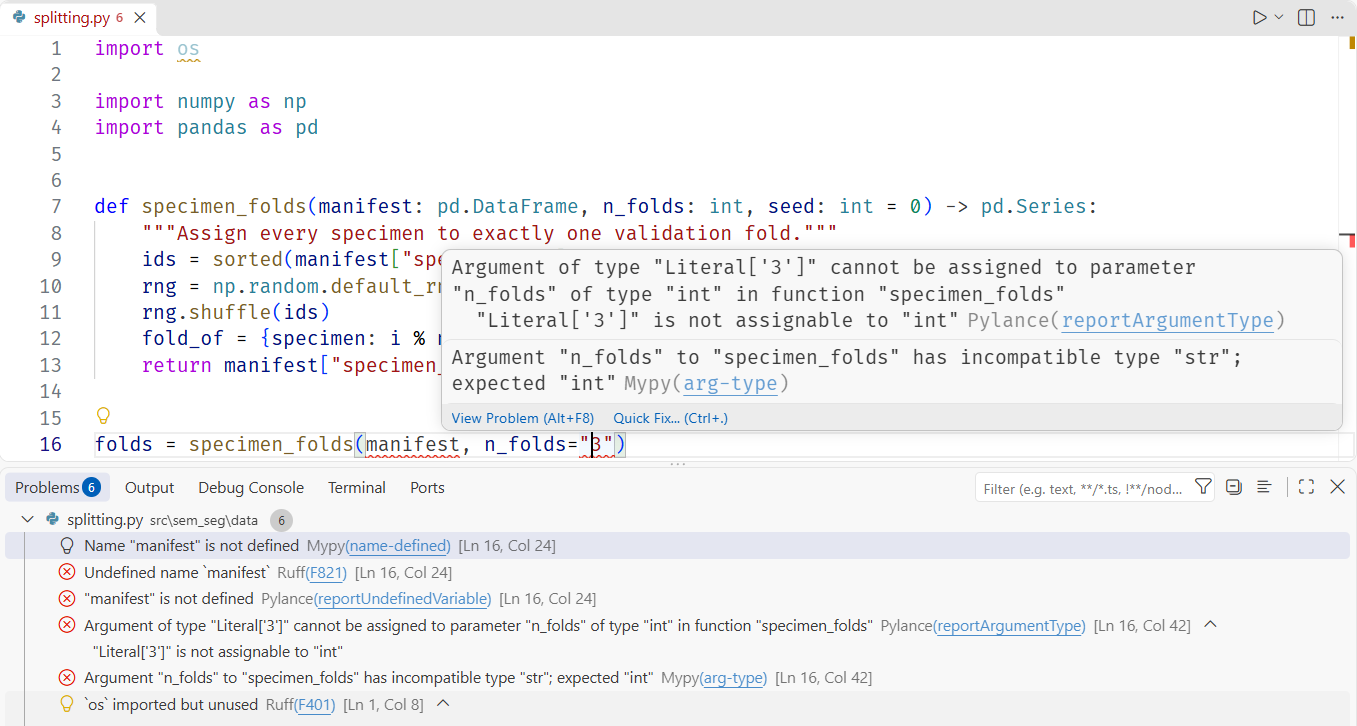
\includegraphics[width=\linewidth]{assets/screens/vscode-lint.png}};
        \begin{scope}[x={(img.south east)},y={(img.north west)}]
          \node[number mark] at (0.179,0.963) {1};
          \node[number mark] at (0.849,0.698) {2};
          \node[number mark] at (0.111,0.328) {3};
        \end{scope}
      \end{tikzpicture}
    \end{column}
    \begin{column}{0.27\textwidth}
      % each item numbered by its marker on the screenshot
      \footnotesize
      \begin{itemize}\setlength\itemsep{2mm}
        \item[\numbermark{1}] Ruff: unused import (\fn{F401}), undefined name (\fn{F821})
        \item[\numbermark{2}] Pylance and mypy: a string passed as \fn{n\_folds}
        \item[\numbermark{3}] Problems panel: every finding, with its tool and rule
      \end{itemize}
    \end{column}
  \end{columns}
  \note{\textbf{8:00--8:40}\par
    A real screenshot: VS Code 1.142 with the Ruff, Pylance and Mypy extensions on a
      deliberately broken version of our split function.\par
    Squiggles mark the unused import, the undefined name and the wrong argument type; hovering
      shows the message and which tool raised it.\par
    The Problems panel lists all six findings, each with its tool and rule, so you can look up
      or switch off a rule.\par
    The agent sees the same findings when it runs the tools from the terminal.}
\end{frame}

% ------------------------------------------------------------ set up once
\begin{frame}[fragile,source={Astral (2026), Ruff: editor setup · Microsoft (2026), Mypy Type Checker; Pylance README}]{Set them up once}
  % left: the tools on the command line; right: the same tools in VS Code. The right column is
  % wide enough for the longest line of settings.json (55 characters at 7 pt) on one line; the
  % left one then holds 42 characters of code and a table whose widest label is "Format".
  \begin{columns}[T,onlytextwidth]
    \begin{column}{0.425\textwidth}
\begin{codefile}[style=sh,basicstyle=\ttfamily\fontsize{7}{8.4}\selectfont]{pyproject.toml}
[tool.ruff]  # rules: Ruff's defaults
line-length = 100

[tool.mypy]
python_version = "3.12"
\end{codefile}
      \scriptsize\renewcommand\arraystretch{1.4}\setlength\tabcolsep{3pt}
      \begin{tabularx}{\linewidth}{@{}>{\bfseries}l>{\ttfamily}X@{}}
        \toprule
        Install        & conda install -c conda-forge ruff mypy\\
        \midrule
        Lint           & ruff check --fix\\
        Format         & ruff format\\
        Types          & mypy src\\
        \bottomrule
      \end{tabularx}
    \end{column}
    \begin{column}{0.545\textwidth}
\begin{codefile}[basicstyle=\ttfamily\fontsize{7}{8.4}\selectfont]{.vscode/settings.json}
{
  "[python]": {
    "editor.defaultFormatter": "charliermarsh.ruff",
    "editor.formatOnSave": true,
    "editor.codeActionsOnSave": {
      "source.fixAll": "explicit",
      "source.organizeImports": "explicit"}},
  "python.analysis.typeCheckingMode": "standard",
  "mypy-type-checker.importStrategy": "fromEnvironment"
}
\end{codefile}
      \footnotesize
      \begin{itemize}\setlength\itemsep{1mm}
        \item VS Code extensions: Python (brings Pylance), Ruff, Mypy Type Checker
        \item pick the environment: \emph{Python: Select Interpreter}
        \item the same commands go into \fn{AGENTS.md}
      \end{itemize}
    \end{column}
  \end{columns}
  \note{\textbf{8:40--9:40}\par
    Set up once per repository, then it runs by itself.\par
    The tool settings live in pyproject.toml, which works for conda projects too.\par
    One conda command installs both; by hand, three commands lint, format and type-check.\par
    In VS Code, install the Python extension, which brings Pylance, plus the Ruff and Mypy Type
      Checker extensions, and select the project's environment.\par
    The workspace settings make Ruff format and fix on every save, switch Pylance's type
      checking on, and make the Mypy extension use the mypy installed in the environment rather
      than the older copy it bundles.\par
    The same commands go into AGENTS.md, so the agent runs them too.}
\end{frame}

\section[Repository]{Preparing the repository}
\sectionframe{03}{Preparing the repository}
  {What can the repository tell the agent, so that we do not have to?}
  {\faFolderOpen}

% ------------------------------------------------------ the layout and its files
% Left: a standard layout, adapted from Cookiecutter Data Science, with one AGENTS.md. Right: the
% same repository later, its AGENTS.md split into three files. One picture, so that the arrow can
% run from one tree to the other: the rows are the theme's folder-tree rows, the pages are drawn
% here. Both trees start at the same height with a row pitch of 3.5 mm; the arrow leaves the
% AGENTS.md row on the left (row 9, y = -12.6 - 8 * 3.5) for rows 5 to 7 on the right.
\begin{frame}[source={DrivenData (2026), Cookiecutter Data Science}]{Setting up the repository}
  \begin{tikzpicture}[x=1mm,y=1mm,
      head/.style={anchor=north west,inner sep=0pt,font=\small\bfseries,text=udsdark},
      page/.style={draw=udsgreylight,fill=white,line width=0.5pt,rounded corners=1.2mm},
      split/.style={udsblue,line width=0.9pt},
      splitarrow/.style={split,-{Stealth[length=2mm,width=1.6mm]}}]
    \useasboundingbox (0,0) rectangle (144,-55);
    % ---- left: the layout, and a link to the template it follows
    \node[head] at (0,0) {A standard layout};
    \node[anchor=north west,inner sep=0pt,font=\footnotesize] at (0,-4.6)
      {\href{https://cookiecutter-data-science.drivendata.org/\#directory-structure}%
        {\faGlobe\enspace\underline{\fn{cookiecutter-data-science}}}};
    \draw[page] (0,-9.4) rectangle (60,-54.4);
    \begin{scope}[shift={(2.4,-12.6)}]
      \treestart{note at=30,row height=3.5}
      \tdir{0}{sem-seg/}{}
      \tdir{1}{data/raw/}{never edited}
      \tdir{1}{data/processed/}{made by the code}
      \tdir{1}{models/}{trained models}
      \tdir{1}{notebooks/}{exploring}
      \tdir{1}{reports/figures/}{figures for papers}
      \tdir{1}{src/sem\_seg/}{the code}
      \tdir{1}{tests/}{}
      \tfile{1}{\textcolor{udsblue}{\textbf{AGENTS.md}}}{\textcolor{udsblue}{for the agent}}
      \tfile{1}{environment.yml}{}
      \tfile{1}{pyproject.toml}{}
      \tfile{1}{README.md}{for people}
    \end{scope}
    % ---- right: the same repository once AGENTS.md has grown; what stays the same in grey
    \node[head] at (74,0) {As the project grows};
    \draw[page] (74,-9.4) rectangle (144,-40.3);
    \begin{scope}[shift={(76.4,-12.6)}]
      \treestart{note at=33.6,row height=3.5}
      \tdir{0}{sem-seg/}{}
      \tdirgrey{1}{data/ \dots}{as before}
      \tdirgrey{1}{models/ \dots\ reports/}{}
      \tdirgrey{1}{src/sem\_seg/, tests/}{}
      \tfile{1}{\textcolor{udsblue}{\textbf{AGENTS.md}}}{commands, rules, pointers}
      \tfile{1}{GLOSSARY.md}{the project's words}
      \tfile{1}{CODING\_STANDARDS.md}{how code is written here}
      \tfilegrey{1}{environment.yml, \dots}{}
    \end{scope}
    \node[anchor=north west,inner sep=0pt,font=\footnotesize,text=udsdark,text width=70mm,
      align=left] at (74,-43.4) {\fn{AGENTS.md} keeps what every session needs and points to
      the two new files};
    % ---- one file becomes three: from the AGENTS.md row on the left to rows 5 to 7 on the right
    \draw[split] (49.5,-40.6) -- (62,-40.6);% starts clear of the note "for the agent"
    \foreach \y in {-26.6,-30.1,-33.6} \draw[splitarrow] (62,-40.6) to[out=0,in=180] (74,\y);
  \end{tikzpicture}
  \note{\textbf{9:50--10:50}\par
    Before any file for the agent: a layout that people and agents already know.\par
    This one follows Cookiecutter Data Science, a template for data projects, with the code in
      src and its tests beside it: raw data that is never edited, processed data that the code
      makes, models, notebooks for exploring, figures for papers.\par
    An agent finds its way in it the way a new colleague does.\par
    At the root sits AGENTS.md, the one file written for the agent.\par
    As the project grows, AGENTS.md keeps what every session needs, and two files take the rest:
      GLOSSARY.md for the project's words, CODING\_STANDARDS.md for how code is written here.}
\end{frame}

% --------------------------------------------------------------- AGENTS.md
% The example file beside what such a file should hold and leave out, after the prompting guides
% of Anthropic and OpenAI (SOURCES.md)
\begin{frame}[fragile,source={Anthropic (2026), Prompting Claude Opus 5.5 · OpenAI (2026), Using GPT-6}]{\texttt{AGENTS.md}}
  \begin{columns}[T,onlytextwidth]
    \begin{column}{0.57\textwidth}
\begin{codefile}[basicstyle=\ttfamily\fontsize{7.2}{8.75}\selectfont]{AGENTS.md}
# sem-seg
## Setup and checks
- Environment: conda env `sem-seg`, activated beforehand
- Fast check (CPU, synthetic data): `pytest -q`
- Lint, types: `ruff check`, `mypy src` §\textcolor{udsred}{\sffamily\scriptsize\faArrowLeft\ after every edit}§
## Conventions
- Terms: `GLOSSARY.md` (specimen, micrograph, patch) §\smash{\textcolor{udsblue}{\faLink}}§
- Decisions: `docs/adr/` §\smash{\textcolor{udsblue}{\faLink}}§
- Lengths in micrometres; pixel size from metadata
## Boundaries
- Never write to `data/raw/`; use `data/processed/`
- No cluster jobs (`sbatch`): the queue is shared
- Ask before adding a dependency
## When you finish
- Report changed files, checks run, open assumptions
\end{codefile}
    \end{column}
    \begin{column}{0.40\textwidth}
      \begin{tikzpicture}[x=1mm,y=1mm,
          head/.style={anchor=north west,inner sep=0pt,font=\footnotesize\bfseries},
          item/.style={anchor=north west,inner sep=0pt,font=\footnotesize,text=udsdark},
          why/.style={anchor=north west,inner sep=0pt,font=\scriptsize,text=udsgrey}]
        \useasboundingbox (0,0) rectangle (57,-54);
        \node[head,text=testgreen] at (0,0) {Put in};
        \foreach \t [count=\i] in {{commands to set up, test and check},
            pointers to what the code cannot show,what needs your approval,
            {when it is done, and what to report},the reason behind a rule}
          \node[item] at (0,-0.7-\i*4.3) {\textcolor{testgreen}{\faCheck}\enspace\t};
        \node[head,text=udsred] at (0,-27.8) {Leave out};
        \foreach \t/\w [count=\i] in {{rules that clash or are out of date}/{the agent may stop and wait},
            {vague wishes: ``write clean code''}/{name the exact mistake instead},
            {``think carefully'', ``be thorough''}/{current models already do}} {
          \node[item] at (0,-25-\i*7.6) {\textcolor{udsred}{\faTimes}\enspace\t};
          \node[why] at (4.3,-28.8-\i*7.6) {\w};
        }
      \end{tikzpicture}
    \end{column}
  \end{columns}
  \note{\textbf{10:50--12:10}\par
    AGENTS.md is the one file that tools supporting it load at the start of every session.\par
    It holds what the agent cannot find out alone: the commands to set up, test and check; what
      the code cannot show, or which file shows it; what needs our approval; when the work is done
      and what to report.\par
    Fifteen lines, each preventing a specific mistake, and one says why: the cluster queue is
      shared.\par
    The checks of section 2 are here, so the agent runs them after every edit; the boundaries are
      requests, not locks.\par
    Today's models follow such files closely: OpenAI notes that its latest model is more
      sensitive to files such as AGENTS.md, and that unclear or conflicting guidance can make it
      stop early.\par
    So leave out rules that clash or are out of date; vague wishes such as write clean code,
      where naming the exact mistake works better; and lines such as think carefully, which
      Anthropic advises removing from system prompts, since the model decides how much to
      think.\par
    Keep it short, and review it like code.}
\end{frame}

% ---------------------------------------------------- glossary, standards
% \tagchip{text}: a tag naming what a file holds
\newcommand\tagchip[1]{\tikz[baseline=(t.base)]\node[draw=udsblue,fill=bluetint,line width=0.4pt,
  rounded corners=0.6mm,inner xsep=1mm,inner ysep=0.5mm,font=\scriptsize,text=udsdark] (t) {#1};}
\begin{frame}[fragile,source={Pocock (2026), mattpocock/skills v1.3.1: domain-modeling, code-review, retro}]{\texttt{GLOSSARY.md} and \texttt{CODING\_STANDARDS.md}}
  \begin{columns}[T,onlytextwidth]
    \begin{column}{0.485\textwidth}
      {\scriptsize\color{udsgrey}holds\enspace}\tagchip{term and meaning}\enspace
        \tagchip{words to avoid}\enspace\tagchip{code name}\par\vskip1.6mm
\begin{codefile}[basicstyle=\ttfamily\fontsize{7}{8.5}\selectfont]{GLOSSARY.md\enspace\textcolor{udsgreymid}{\sffamily\scriptsize read when pointed to}}
# Glossary
Specimen: one physical sample (`specimen_id`).
  Avoid: §\textcolor{udsred}{\bfseries sample}§, coupon. §\textcolor{udsred}{\sffamily\scriptsize\faArrowLeft\ the word in our request}§
Area: one imaged region of a specimen.
Micrograph: one SEM image of an area
  (`micrograph_id`). Avoid: image, frame.
Patch: a crop of a micrograph used in
  training (`patch_id`). Avoid: tile.
Fold: specimens held out together; every
  specimen belongs to exactly one fold.
\end{codefile}
    \end{column}
    \begin{column}{0.485\textwidth}
      {\scriptsize\color{udsgrey}holds\enspace}\tagchip{seeds}\enspace\tagchip{input checks}\enspace
        \tagchip{tests}\enspace\tagchip{paths}\par\vskip1.6mm
\begin{codefile}[basicstyle=\ttfamily\fontsize{7}{8.5}\selectfont]{CODING\_STANDARDS.md\enspace\textcolor{udsgreymid}{\sffamily\scriptsize read in review}}
# Coding standards
- Every random step takes a `seed`; the
  same seed gives the same result.
- Public functions check their inputs and
  raise `ValueError` naming the problem.
- Tests call public functions on small,
  hand-written fixtures, never real data.
- Expected values come from the fixture,
  never recomputed the way the code does.
- Paths come from `config.py`, never
  written into a function.
\end{codefile}
    \end{column}
  \end{columns}
  \note{\textbf{12:10--13:30}\par
    Two files the agent reads only when something points to them.\par
    A glossary holds the project's terms: what each one means, the words to avoid and the name the
      code uses for it; our request said sample, and here sample is a word to avoid.\par
    The clarifying step of section 7 writes terms into it as soon as they are agreed.\par
    Coding standards hold the rules a reviewer checks: seeds, input checks, how tests are built,
      where paths come from; a fixture is the small, hand-made input a test runs on.\par
    In the workflow of section 7 the review step reads it, not the implementing agent, which
      already carries the most context.\par
    Rules that a linter can check belong in Ruff's settings instead, so that every run checks
      them.}
\end{frame}

\section[Decisions]{Architecture Decision Records (ADRs)}
\sectionframe{04}{Architecture Decision Records (ADRs)}
  {Why does the project work this way, and what if we change our minds?}
  {\faBalanceScale}

% ------------------------------------------------------------ what / when
\begin{frame}[source={Nygard (2011), Documenting architecture decisions · Pocock (2026), mattpocock/skills v1.3.1, domain-modeling}]{What an ADR is, and when to write one}
  \begin{tikzpicture}[x=1mm,y=1mm,
      crit/.style={inner sep=0pt,font=\footnotesize,text=udsdark,align=center},
      item/.style={anchor=base west,inner sep=0pt,font=\footnotesize,text=udsdark}]
    % the record itself: Nygard's format
    \node[anchor=north west,inner sep=0pt,font=\footnotesize,text=udsdark] at (0,0)
      {\textbf{One decision per record:}\enspace title · context · decision · status ·
       consequences; numbered; superseded records stay};
    % write one only where all three hold; each label sits in its circle's own part
    \coordinate (A) at (17,-22); \coordinate (B) at (35,-22); \coordinate (C) at (26,-37.6);
    \foreach \p in {A,B,C}
      \filldraw[draw=udsblue,line width=0.7pt,fill=udsblue,fill opacity=0.09] (\p) circle (15);
    \node[crit] at (11.5,-19.5) {hard to\\reverse};
    \node[crit] at (40.5,-19.5) {surprising\\without\\context};
    \node[crit] at (26,-44) {a real\\trade-off};
    \node[inner sep=0.4mm,font=\small\bfseries,text=udsred] (adr) at (26,-27.2) {ADR};
    % where all three usually hold in research code, level with the circles' top
    \node[anchor=north west,inner sep=0pt,font=\footnotesize\bfseries,text=udsdark] at (70,-7)
      {typical in research code};
    \foreach \t [count=\i] in {the split unit and the evaluation protocol,merged or remapped classes,
        {units, scales, normalisation},the metric that decides what is ``better''}
      \node[item] at (72,-9.2-\i*5.4) {\textcolor{udsred}{\faAngleRight}\enspace\t};
    \draw[udsred,line width=0.6pt] (adr.east) to[out=0,in=180] (69.4,-21.7);
    \node[anchor=base west,inner sep=0pt,font=\scriptsize,text=udsgrey] at (72,-41)
      {no ADR: plot styling, renames};
  \end{tikzpicture}
  \note{\textbf{13:40--14:40}\par
    An architecture decision record keeps one decision with its reasons.\par
    Nygard's format: title, context, decision, status and consequences, including the bad
      ones.\par
    Records are numbered in sequence, numbers are never reused, and a superseded record stays in
      the repository.\par
    A useful test, from the skills of section 7: write one only when the decision is hard to
      reverse, would surprise a newcomer, and came from a real trade-off.\par
    In research code that is usually about what a number means: the split unit, class
      definitions, units and normalisation, the metric.\par
    Plot styling and renames do not need one.}
\end{frame}

% ------------------------------------------------------------- ADR example
\begin{frame}[fragile]{ADR-0003: specimen-level splits}
  \begin{columns}[T,onlytextwidth]
    \begin{column}{0.58\textwidth}
\begin{codefile}[basicstyle=\ttfamily\fontsize{7}{8.4}\selectfont]{docs/adr/0003-specimen-level-splits.md}
# ADR-0003: Specimen-level splits
Status: accepted. Supersedes ADR-0001 (random patch split).
## Context
Micrographs of one specimen share preparation and etching;
several show the same area. A random patch split puts this
material in training and validation.
## Decision
Specimens are assigned to validation folds; each patch
inherits its specimen's fold. Folds are saved with seed
and manifest hash and checked for overlap.
## Considered options
Random patch split; split by micrograph. Both leak.
## Consequences
Few independent units: report every fold and its spread.
One specimen per state: a held-out specimen is a new state.
\end{codefile}
    \end{column}
    \begin{column}{0.39\textwidth}
      \begin{tikzpicture}[x=1mm,y=1mm]
        \node[artifact,anchor=north west,text width=50mm,align=left,font=\scriptsize] (a1) at (0,0)
          {\texttt{0001-random-patch-split.md}\\[0.4mm]
           \textcolor{udsred}{Status: superseded by ADR-0003}};
        \node[artifact,anchor=north west,text width=50mm,align=left,font=\scriptsize,draw=udsblue,fill=bluetint] (a3) at (0,-16)
          {\texttt{0003-specimen-level-splits.md}\\[0.4mm]
           \textcolor{udsblue}{Status: accepted}};
        \draw[flow] (a3.north) -- node[lbl,right]{supersedes} (a1.south);
        \node[anchor=north west,text width=54mm,font=\scriptsize,inner sep=0pt] at (0,-27.5)
          {ADR-0001 stays: it shows what was tried and why it changed.};
      \end{tikzpicture}\par\vskip3mm
      \begin{panel}[fontupper=\footnotesize,colback=bluetint,borderline west={1.2mm}{0pt}{udsblue},left=3.5mm]
        An agent chasing a better score finds ADR-0003 through \fn{AGENTS.md} before it brings back a
        random split.
      \end{panel}
    \end{column}
  \end{columns}
  \note{\textbf{14:40--15:40}\par
    The record for our running example.\par
    The context explains why a random patch split misleads here; the decision is short and
      testable; the considered options show that splitting by micrograph was rejected for the
      same reason.\par
    The consequences are honest: few specimens mean few independent units, and with one specimen
      per material state every held-out specimen is also a new state.\par
    ADR-0001 is not deleted; its status points to its successor.\par
    An agent tuning for a better score finds this record before it undoes the decision.}
\end{frame}

% ------------------------------------------------------------- file roles
\begin{frame}[source={OpenAI (2026), Custom instructions with AGENTS.md · Pocock (2026), mattpocock/skills v1.3.1: code-review; v1.3 changelog}]{When the agent reads each file}
  % the files of sections 3 and 4, the README and the task specification of section 1, placed on
  % an agent session at the moment each one is read
  \begin{tikzpicture}[x=1mm,y=1mm,
      chip/.style={draw=udsgreylight,fill=white,rounded corners=0.6mm,inner xsep=1mm,inner ysep=0.8mm,
        anchor=north west,font=\ttfamily\fontsize{7.4}{8.4}\selectfont,text=udsdark,line width=0.5pt,
        path picture={\draw[udsblue,line width=0.9pt] (path picture bounding box.north west)
          -- (path picture bounding box.north east);}},
      always/.style={chip,draw=udsblue,line width=0.9pt},
      ondemand/.style={chip,dashed,draw=udsdark,path picture={}},
      reviewstep/.style={chip,draw=udsblue,fill=bluetint,path picture={},font=\footnotesize},
      say/.style={anchor=north west,inner sep=0pt,font=\scriptsize,text=udsdark,align=left,text width=30mm,
        execute at begin node={\hyphenpenalty=10000\raggedright}},
      drop/.style={udsgreymid,line width=0.5pt},
      dot/.style={circle,fill=udsdark,inner sep=0pt,minimum size=1.8mm}]
    % AGENTS.md points to the glossary and the ADRs
    \node[always] (ag) at (0,-4.6) {AGENTS.md};
    \node[ondemand] (gl) at (44,-4.6) {GLOSSARY.md};
    \node[ondemand] (ad) at (78,-4.6) {docs/adr/};
    \draw[drop,dashed] (ag.north) |- (ad.north |- 0,-1.6);
    \foreach \n in {gl,ad} \draw[drop,dashed,-{Stealth[length=1.6mm,width=1.2mm]}] (\n.north |- 0,-1.6) -- (\n.north);
    \node[anchor=south,inner sep=0.5mm,font=\scriptsize,text=udsgrey,fill=white] at (27,-1.6) {points to};
    \node[say] at ([yshift=-1.2mm]ag.south west) {\textcolor{udsblue}{\bfseries every session}\\ commands, boundaries, pointers};
    \node[say] at ([yshift=-1.2mm]gl.south west) {\textbf{when pointed to}\\ domain terms};
    \node[say] at ([yshift=-1.2mm]ad.south west) {\textbf{when pointed to}\\ one decision and its reasons};
    % read in review
    \node[chip] (cs) at (112,-4.6) {CODING\_STANDARDS.md};
    \node[say] at ([yshift=-1.2mm]cs.south west) {\textbf{in review}\\ how code is written here};
    % the session, left to right, and where each file enters it
    \draw[flow,line width=0.9pt] (0,-27) -- (143.4,-27);% the tip stays inside the text width
    \node[anchor=south west,inner sep=0.6mm,font=\scriptsize,text=udsgrey] at (12,-27) {an agent session};
    \foreach \n in {ag,gl,ad,cs} {\node[dot] at (\n.south |- 0,-27) {}; \draw[drop] (\n.south |- 0,-21.6) -- (\n.south |- 0,-27);}
    % the task's own specification comes with it; the review checks the code against the standards
    \node[chip,font=\footnotesize] (sp) at (0,-32) {task specification};
    \node[say] at ([yshift=-1.2mm]sp.south west) {\textbf{with the task}\\ objective, acceptance criteria};
    \draw[drop] (ag.south |- 0,-27) -- (ag.south |- sp.north);
    \node[reviewstep] (cr) at (112,-32) {\faSearch\enspace review};
    \node[say] at ([yshift=-1.2mm]cr.south west) {a person or an agent checks the code against it};
    \draw[drop] (cs.south |- 0,-27) -- (cs.south |- cr.north);
    % read like any other file
    \node[chip,draw=udsgreylight,text=udsgrey,path picture={}] (rd) at (44,-34) {README.md};
    \node[say,text=udsgrey,text width=40mm,anchor=west] at ([xshift=2mm]rd.east) {for people; read like any other file};
  \end{tikzpicture}
  \note{\textbf{15:40--16:30}\par
    Each file on one agent session, at the moment it is read.\par
    AGENTS.md at the start of every session; the glossary and the ADRs when AGENTS.md points to
      them.\par
    The task specification of section 1 comes with the task; the coding standards are read when
      the change is reviewed, by a person or an agent.\par
    The README is for people; the agent reads it like any other file.\par
    Keep each fact in one place and link to it: copies go stale.}
\end{frame}

% ------------------------------------ the specification of section 1, remembered
% Slide 5's five cards again, greyed: the theme's colours are redefined for one group only, so the
% same macros draw them. A stamp repeats slide 5's warning; the strip says where the parts that
% repeat are now, which the next slide shows card by card.
\begin{frame}{Remember the bounded task specification?}
  \begin{tikzpicture}[x=1mm,y=1mm]
    \useasboundingbox (0,0) rectangle (144,-54);
    \begingroup
      \colorlet{udsblue}{udsgreymid}\colorlet{udsdark}{udsgreymid}
      \foreach \k/\l in {0/Objective,1/Context,2/Constraints,3/Acceptance,4/Verification}
        {\speccard{\k}{0}{-41.4}{\l}{udsgreypale!60}}
      \foreach \k/\t in {
          0/{add \fn{specimen\_folds()} to \fn{src/sem\_seg/\allowbreak data/\allowbreak splitting.py}; use it
            in the training CLI as \fn{--split specimen}},
          1/{``sample'' means specimen: one physical sample, column \fn{specimen\_id} of the manifest},
          2/{leave \fn{data/raw/} and the manifests unchanged; no new dependencies; no GPU jobs},
          3/{each specimen in exactly one fold; each patch inherits its specimen's fold; same seed, same
            folds; \fn{ValueError} if \fn{specimen\_id} is missing or there are fewer specimens than folds},
          4/{\fn{pytest tests/data -q} passes; report changed files, test output and assumptions}}
        \node[spec body] at (b\k) {\t};
    \endgroup
    % slide 5's warning, stamped across the cards
    \node[rotate=7,draw=udsred,double=white,double distance=0.7pt,line width=0.8pt,
      rounded corners=1mm,fill=white,fill opacity=0.88,text opacity=1,text=udsred,
      font=\large\bfseries,inner xsep=3mm,inner ysep=2.2mm] at (72,-21)
      {\faExclamationTriangle\enspace too much to write for every task};
    % where those parts are now
    \fill[bluetint] (0,-48.4) rectangle (144,-54);
    \fill[udsblue] (0,-48.4) rectangle (1.2,-54);
    \node[anchor=west,inner sep=0pt,font=\footnotesize,text=udsdark] at (3.6,-51.2)
      {\textcolor{udsblue}{\faCheck}\enspace what repeats is now in files: \fn{AGENTS.md},
       \fn{GLOSSARY.md}, ADRs, \fn{CODING\_STANDARDS.md}};
  \end{tikzpicture}
  \note{\textbf{16:30--17:00}\par
    Remember the bounded specification from the start of the talk.\par
    Every part of it was written by hand, for every task: what a specimen is, which data must not
      change, how to run the tests, what to report.\par
    That is the part that repeats, and it now lives in the files of sections 3 and 4.}
\end{frame}

% ------------------------------------------------ the request, revisited
\begin{frame}{The same request, in a prepared repository}
  \begin{tikzpicture}[x=1mm,y=1mm]
    % the cards fill the text width exactly; strokes on their edges must not widen the picture
    \useasboundingbox (0,0) rectangle (144,-54);
    \specterminal{0}{the request}
    \node[spec request] at (term) {> Add validation folds by specimen to the training CLI, as decided in ADR-0003.};
    \node[anchor=west,inner sep=0pt,font=\scriptsize\bfseries,text=udsdark] at (0,-15.8)
      {where the rest comes from};
    % the same five cards as on slides 4 and 5: the objective is the request itself, every other
    % part now comes from files
    \speccard{0}{-19}{-44.4}{Objective}{darktint}
    \foreach \k/\l in {1/Context,2/Constraints,3/Acceptance,4/Verification}
      {\specfilecard{\k}{-19}{-44.4}{\l}{darktint}}
    \node[spec chip,draw=termbg,fill=termbg,text=termfg,path picture={}] at (b0) {\faTerminal\ the request};
    % context
    \node[spec chip] (c1) at (b1) {GLOSSARY.md};
    \node[spec note] (c1s) at ([yshift=-0.8mm]c1.south west) {specimen, fold};
    \node[spec chip] (c2) at ([yshift=-2.2mm]c1s.south west) {ADR-0003};
    \node[spec note] at ([yshift=-0.8mm]c2.south west) {why; how folds are saved};
    % constraints
    \node[spec chip] (k1) at (b2) {AGENTS.md};
    \node[spec note] at ([yshift=-0.8mm]k1.south west) {boundaries};
    % acceptance
    \node[spec chip] (a1) at (b3) {ADR-0003};
    \node[spec note] (a1s) at ([yshift=-0.8mm]a1.south west) {one fold per specimen};
    \node[spec chip] (a2) at ([yshift=-2.2mm]a1s.south west) {CODING\_STANDARDS.md};
    \node[spec note] at ([yshift=-0.8mm]a2.south west) {seed, input checks};
    % verification
    \node[spec chip] (v1) at (b4) {AGENTS.md};
    \node[spec note] at ([yshift=-0.8mm]v1.south west) {fast check, report};
    % what the files leave open, the agent has to ask: the clarifying step of section 7
    \node[anchor=west,inner sep=0pt,font=\scriptsize,text=udsred] at (0,-49.4)
      {\faQuestionCircle\enspace still open: what no file says, e.g.\ the default number of folds};
  \end{tikzpicture}
  \note{\textbf{17:00--18:00}\par
    Now the same request, in the repository we prepared.\par
    With these files in place, one sentence in the project's language is enough.\par
    Four of the five parts now come from files; only the objective is in the request.\par
    The glossary says what a specimen and a fold are.\par
    ADR-0003 says why folds go by specimen and how they are saved.\par
    AGENTS.md carries the boundaries, the test command and what to report.\par
    CODING\_STANDARDS.md makes seeds and input checks part of every review.\par
    What the files leave open, here the default number of folds, is what the clarification step
      of section 7 asks.\par
    This works only while AGENTS.md points to the files and they are kept current.}
\end{frame}

\section[Version control]{Version control with git}
\sectionframe{05}{Version control with git}
  {How do we keep every version, and see exactly what an agent changed?}
  {\faCodeBranch}

% ------------------------------------------------------------- what it is
\begin{frame}[source={Chacon \& Straub (2014), Pro Git, 2nd ed., git-scm.com/book}]{Version control: one folder, every version}
  \begin{columns}[T,onlytextwidth]
    \begin{column}{0.34\textwidth}
      \begin{ablock}[equal height group=vc,fontupper=\footnotesize]{Without}
        {\ttfamily\footnotesize splitting.py\\ splitting\_old.py\\ splitting\_v2\_final.py\\
         splitting\_v2\_final\_FIXED.py\\ results\_new2/\par}\vskip2mm
        Which version produced figure 3?
      \end{ablock}
    \end{column}
    \begin{column}{0.62\textwidth}
      \begin{dblock}[equal height group=vc,fontupper=\footnotesize]{With git}
        \centering
        \begin{tikzpicture}[x=1mm,y=1mm,
            commit/.style={circle,draw=udsblue,fill=white,line width=0.9pt,minimum size=3mm,inner sep=0pt},
            bcommit/.style={commit,draw=udsred},
            msg/.style={font=\scriptsize,text=udsdark,inner sep=0.6mm}]
          \draw[udsblue,line width=1pt] (0,0) -- (51,0);
          \draw[udsred,line width=1pt] (14,0) to[out=0,in=180] (23,9) -- (42,9) to[out=0,in=180] (51,0);
          \foreach \n/\x/\t in {a/0/random split,b/14/checks,m/51/merge} {
            \node[commit] (\n) at (\x,0) {};
            \node[msg,anchor=north] at (\n.south) {\t};
          }
          \foreach \n/\x/\t in {e/25/specimen folds,f/40/tests} {
            \node[bcommit] (\n) at (\x,9) {};
            \node[msg,anchor=south] at (\n.north) {\t};
          }
          \node[font=\scriptsize\bfseries,text=udsblue,anchor=east] at (-2.5,0) {main};
        \end{tikzpicture}\par\vskip1.5mm
        \raggedright\renewcommand\arraystretch{1.15}\setlength\tabcolsep{3pt}
        \begin{tabular}{@{}>{\bfseries}l l@{}}
          commit & a snapshot with a message, an author and a date\\
          diff   & what changed between two snapshots\\
          \textcolor{udsred}{branch} & a separate line of work, merged when ready\\
          remote & a copy on a server (GitHub): backup, sharing, review\\
        \end{tabular}
      \end{dblock}
    \end{column}
  \end{columns}
  \note{\textbf{18:10--19:20}\par
    Many of us keep versions as copies: splitting old, v2, final, fixed.\par
    After a few months nobody knows which copy produced a figure.\par
    Version control replaces the copies with one folder and its history.\par
    Git stores a snapshot of the project each time you commit, with a message, an author and a
      date; a diff shows what changed between two snapshots.\par
    A branch is a separate line of work, for an experiment or for an agent's task, merged back
      when it is ready.\par
    A remote such as GitHub holds a copy of the history on a server: a backup, a way to share,
      and the place where changes are reviewed.\par
    There a branch comes back as a pull request: a request to merge it, with its diff open for
      review before it reaches main.}
\end{frame}

% ------------------------------------------------------- learning curve
\begin{frame}[fragile,source={Chacon \& Straub (2014), Pro Git, 2nd ed., git-scm.com/book · Microsoft (2026), VS Code docs: Source control}]{Getting started takes five commands}
  \edef\colgap{\the\dimexpr0.04\textwidth\relax}
  \begin{columns}[T,onlytextwidth]
    \begin{column}{0.55\textwidth}
\begin{terminal}[basicstyle=\ttfamily\fontsize{7.2}{9.2}\selectfont]{terminal}
$ git init              # once: start the history
$ git status            # what has changed?
$ git add src/ tests/   # choose what goes in
$ git commit -m "Split by specimen"
$ git push              # copy it to GitHub
\end{terminal}
      \vskip1mm
\begin{codefile}[style=sh,basicstyle=\ttfamily\fontsize{7.2}{9.2}\selectfont]{.gitignore}
data/          # raw and derived data stay out
.venv/         # environments are rebuilt, not stored
*.ckpt         # model checkpoints
.env           # secrets
.claude/worktrees/  # agent worktrees
\end{codefile}
    \end{column}
    \begin{column}{0.41\textwidth}
      \begin{tikzpicture}
        \node[anchor=south west,inner sep=0pt,draw=udsgreylight,line width=0.4pt] (img) at (0,0)
          {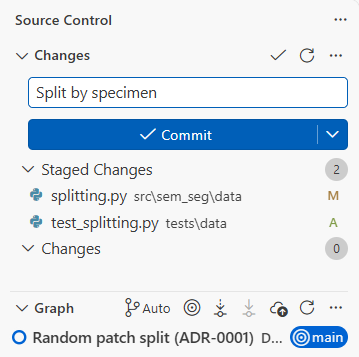
\includegraphics[height=36mm]{assets/screens/vscode-scm.png}};
        % each control, labelled with the command it replaces; push is the cloud button of the
        % graph's title row, so its line starts under that button and passes below the row
        \begin{scope}[x={(img.south east)},y={(img.north west)},
            cmd/.style={right,inner sep=0.6mm,font=\ttfamily\scriptsize,text=udsdark}]
          \foreach \y/\t in {0.683/commit,0.521/add,0.412/status}
            \draw[udsgreymid,line width=0.5pt] (1,\y) -- ++(2.5mm,0) node[cmd] {git \t};
          \draw[udsgreymid,line width=0.5pt] (0.79,0.112) |- (1,0.1) -- ++(2.5mm,0)
            node[cmd] {git push};
        \end{scope}
      \end{tikzpicture}\par\vskip1mm
      {\scriptsize VS Code's Source Control panel does the same with clicks.\par}\vskip2mm
      % the arrow spans the gap between the columns (0.04 of the text width), so it starts at the
      % edge of .gitignore; drawn by the box itself, it also lands right in the notes thumbnails
      \begin{panel}[colback=redtint,borderline west={1.2mm}{0pt}{udsred},left=3.5mm,fontupper=\footnotesize,
          overlay={\draw[flow] ([xshift=-\colgap]frame.west) -- (frame.west);}]
        data, environments and secrets do not belong in the history
      \end{panel}
    \end{column}
  \end{columns}
  \note{\textbf{19:20--20:20}\par
    The learning curve is shorter than its reputation.\par
    Five commands cover daily use: start the history once, check what changed, choose what goes
      into the next snapshot, commit it with a message, and push it to GitHub, the remote of the
      last slide.\par
    VS Code's Source Control panel does the same with buttons: here two files are staged, the
      message is typed, one click on Commit, and the cloud button pushes; the graph below is the
      history.\par
    The first push needs a repository on GitHub to push to; that cloud button, Publish Branch,
      creates one and pushes.\par
    A .gitignore file keeps out what does not belong in the history: data, environments, which
      are rebuilt from their description, model checkpoints, secrets, and the worktrees that Claude
      Code creates.\par
    Branches and merges can come later.}
\end{frame}

% ------------------------------------------------------- git and agents
\begin{frame}[source={OpenAI (2026), Agent approvals and security; Non-interactive mode · Anthropic (2026), Claude Code checkpointing}]{Why an agent needs version control}
  \begin{columns}[T,onlytextwidth]
    \begin{column}{0.66\textwidth}
      \begin{tikzpicture}
        \node[anchor=south west,inner sep=0pt,draw=udsgreylight,line width=0.4pt] at (0,0)
          {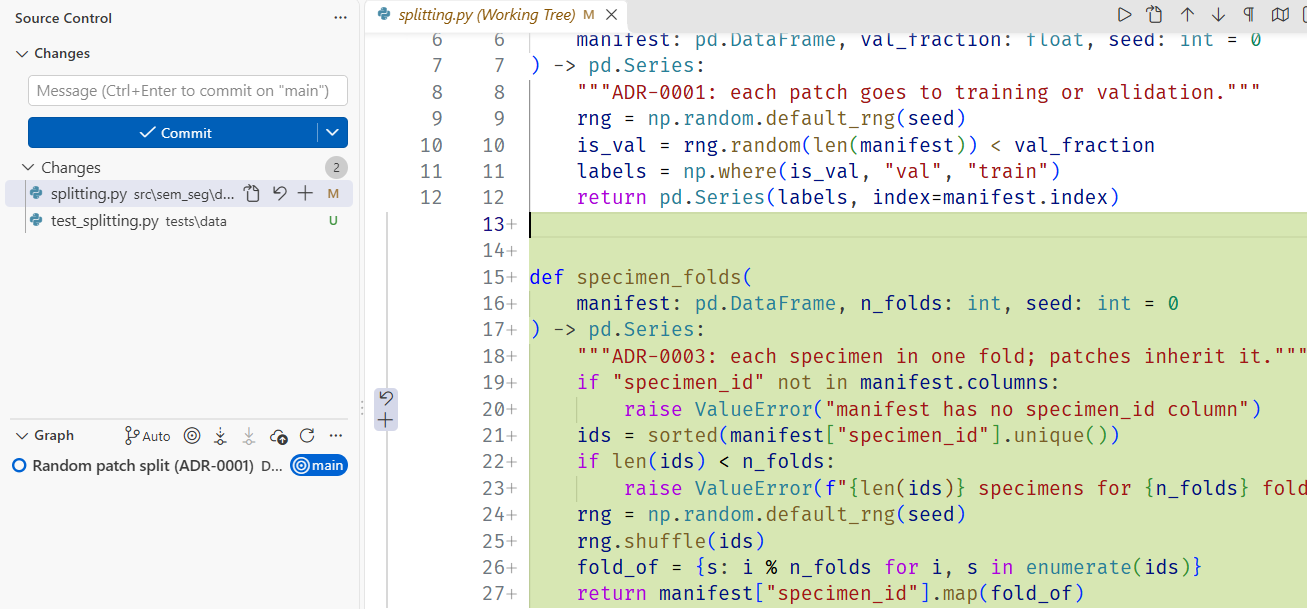
\includegraphics[width=\linewidth]{assets/screens/vscode-git.png}};
      \end{tikzpicture}\par\vskip1mm
      {\scriptsize An agent's change in VS Code's Source Control view: two files, every new line in green.\par}
    \end{column}
    \begin{column}{0.31\textwidth}
      \begin{tikzpicture}[x=1mm,y=1mm,
          commit/.style={circle,draw=udsblue,fill=white,line width=0.9pt,minimum size=3.4mm,inner sep=0pt},
          gitstep/.style={anchor=base west,inner sep=0pt,font=\footnotesize,text=udsdark,align=flush left,
            text width=38.6mm}]
        \useasboundingbox (0,0) rectangle (44.6,-52);
        % a checkpoint, the agent's uncommitted edits, then keep or discard them;
        % each label's first baseline sits 1 mm below its circle's centre
        \draw[udsblue,line width=0.9pt] (1.7,-1.9) -- (1.7,-14.4);
        \node[commit] at (1.7,-1.9) {};
        \node[gitstep] at (6,-2.9) {\textbf{checkpoint}\\commit before the agent starts};
        \node[commit,draw=udsred,dashed] (e) at (1.7,-14.4) {};
        \node[gitstep] at (6,-15.4) {\textbf{the agent's edits}\\read the diff, not the summary};
        \draw[udsblue,line width=0.9pt] (e.south) to[out=-90,in=180] (6,-27);
        \node[commit] at (7.7,-27) {};
        \node[gitstep,text width=33mm] at (11.6,-28)
          {\textbf{keep}\enspace\fn{git commit}\\{\color{udsgrey}undo later: \fn{git revert}}};
        \draw[udsgreymid,line width=0.9pt,dashed] (e.south) to[out=-90,in=180] (6,-38.6);
        \node[circle,fill=udsgreymid,text=white,inner sep=0pt,minimum size=3.4mm,font=\tiny]
          at (7.7,-38.6) {\faTimes};
        \node[gitstep,text width=33mm] at (11.6,-39.6)
          {\textbf{discard}\enspace\fn{git restore}\\{\color{udsgrey}the edits are lost}};
        \node[gitstep,text width=44.6mm,font=\footnotesize\bfseries,text=udsblue] at (0,-50.4)
          {one branch or worktree per task};
      \end{tikzpicture}
    \end{column}
  \end{columns}
  \note{\textbf{20:20--21:30}\par
    With git, an agent's work becomes a diff we can read before we accept it.\par
    Commit before the agent starts, so there is a checkpoint to return to.\par
    Read the diff itself, not the agent's summary of it: here, two files, every added line in
      green.\par
    Undo is one command: restore discards uncommitted changes for good, revert undoes a commit
      and keeps the history.\par
    A branch, or a separate worktree, per task keeps an agent's work apart from ours until it is
      reviewed.\par
    The tools assume all this.\par
    Codex checks at launch whether the folder is under version control, suggests read-only mode
      when it is not, and codex exec refuses to run outside a repository unless told
      otherwise.\par
    Claude Code can rewind its own file edits, but not files changed by shell commands, and its
      documentation says to keep using git.\par
    The workflow of section 7 commits each finished piece of work, and its review compares
      against a commit.}
\end{frame}

% ------------------------------------------------------------- worktrees
\begin{frame}[fragile,source={git documentation (2026), git-worktree · Anthropic Academy (2026)}]{Worktrees: work in parallel, merge when done}
  % the drawing carries the ideas; what a worktree is and its three commands sit beside it, level
  % with its middle
  \begin{columns}[c,onlytextwidth]
    \begin{column}{0.34\textwidth}
      \footnotesize
      \begin{itemize}\setlength\itemsep{1.5mm}
        \item a worktree: another folder of the same repository, on its own branch
        \item all folders share one history, so each branch merges into \fn{main}
      \end{itemize}\vskip2.5mm
\begin{terminal}[basicstyle=\ttfamily\fontsize{7.2}{8.5}\selectfont]{terminal}
$ git worktree add ../folds \
    -b agent/folds
$ git worktree list
$ git worktree remove ../folds
\end{terminal}
    \end{column}
    \begin{column}{0.63\textwidth}
      \centering
      \begin{tikzpicture}[x=1mm,y=1mm,
          pill/.style={rounded corners=2mm,minimum height=4mm,inner xsep=2mm,inner ysep=0.4mm,
            font=\fontsize{7}{8}\selectfont\bfseries,text=white},
          dot/.style={circle,inner sep=0pt,minimum size=2.4mm},
          tie/.style={udsgreylight,dashed,line width=0.5pt},
          card/.style={draw=udsblue,fill=bluetint,line width=0.6pt,rounded corners=1mm,
            align=left,font=\scriptsize,inner xsep=1.6mm,inner ysep=1.2mm}]
        % branches first, so that dots and cards sit on top of them
        \draw[udsblue,line width=1pt] (68,3) to[out=135,in=270] (55,20) to[out=90,in=235] (68,31);
        \draw[udsblue,line width=1pt] (68,3) to[out=162,in=270] (27,20) to[out=90,in=200] (68,42);
        \draw[udsdark,line width=1.2pt,-{Stealth[length=2.4mm,width=1.8mm]}] (68,0) -- (68,46);
        % your own folder, on main
        \node[card,draw=udsred,fill=redtint,anchor=south] at (68,46.6)
          {{\color{udsred}\faFolderOpen}\ \textbf{\fn{sem-seg/}}\quad\faCodeBranch\ \fn{main}\quad\faUser\ you};
        % commits on main, on the right; the two merges in red
        \foreach \y/\t/\c in {3/commit/udsdark,14/your commit/udsdark,31/merge/udsred,42/merge/udsred} {
          \node[dot,fill=\c] at (68,\y) {};
          \draw[tie] (69.5,\y) -- (72,\y);
          \node[pill,fill=\c,anchor=west] at (72,\y) {\t};
        }
        % one worktree per branch: its folder, its branch, its agent
        \foreach \x/\n/\b in {55/1/folds,27/2/check} {
          \node[dot,fill=udsblue] at (\x,20) {};
          \draw[tie] (\x-1.5,20) -- (\x-3,20);
          \node[card,anchor=east] at (\x-3,20)
            {{\color{udsblue}\faFolderOpen}\ \textbf{\fn{../\b}}\\ \faCodeBranch\ \fn{agent/\b}\\ \faRobot\ agent \n};
        }
      \end{tikzpicture}
    \end{column}
  \end{columns}
  \note{\textbf{21:30--22:30}\par
    A worktree is a second working folder of the same repository, checked out on its own
      branch.\par
    Each card is one: a folder next to the repository, its branch, and the agent working in it;
      your own folder, sem-seg, is the main worktree on main.\par
    Both agents start from the same commit on main and work at the same time, while you keep
      committing on main in your own folder.\par
    When an agent's work is reviewed, its branch is merged into main: first one, then the
      other.\par
    All worktrees share one history, and git lets a branch be checked out in only one worktree
      at a time, so the agents get in neither each other's way nor yours.\par
    Three commands: add creates the folder and the branch, list shows them, remove deletes the
      folder once its branch is merged.}
\end{frame}

% ------------------------------------------- worktrees in the app and the terminal
\begin{frame}[source={Anthropic (2026), Claude Code docs: Desktop; Worktrees; CLI reference}]{How to use worktrees?}
  \begin{tikzpicture}[x=1mm,y=1mm,
      head/.style={anchor=north west,inner sep=0pt,font=\small\bfseries,text=udsdark},
      stage/.style={circle,fill=udsblue,text=white,inner sep=0pt,minimum size=5.6mm,font=\scriptsize},
      txt/.style={anchor=north west,inner sep=0pt,font=\footnotesize,text=udsdark,align=flush left,
        text width=61mm},
      mono/.style={anchor=west,inner sep=0pt,font=\ttfamily\fontsize{7}{8}\selectfont}]
    \useasboundingbox (0,0) rectangle (144,-55);
    \node[head] at (8,0) {Claude app};
    \node[head] at (83,0) {Terminal};
    \draw[udsgreylight,line width=0.4pt] (72,0) -- (72,-54.6);
    % the app: Worktree on under the prompt box (screenshot), with a red box on the button
    \node[anchor=north west,inner sep=0pt,draw=udsgreylight,line width=0.4pt] (app) at (8,-4.6)
      {
\includegraphics[width=61mm]{assets/screens/claude-app-worktree.png}};
    \begin{scope}[shift={(app.south west)},x={($(app.south east)-(app.south west)$)},
        y={($(app.north west)-(app.south west)$)}]
      \draw[udsred,line width=1.1pt] (0.552,0.01) rectangle (0.809,0.35);
    \end{scope}
    % the terminal: the session's own branch, as Claude Code shows it
    \fill[termbg,rounded corners=1.2mm] (83,-4.6) rectangle (144,-19.04);
    \foreach \c [count=\i] in {termdot1,termdot2,termdot3} \fill[\c] (83.4+\i*2.3,-7.2) circle (0.7);
    \node[inner sep=0pt,font=\ttfamily\fontsize{7}{8}\selectfont,text=termdim] at (113.5,-7.2)
      {claude --worktree specimen-folds};
    \draw[white!18!termbg,line width=0.4pt] (83,-9.8) -- (144,-9.8);
    \node[mono,text=termfg] at (85.6,-12.9) {! git branch --show-current};
    \node[mono,text=termfg] at (85.6,-16.4) {\phantom{! }└ worktree-specimen-folds};
    \draw[udsred,line width=1.1pt] (84.6,-10.9) rectangle (124.4,-18.4);
    \node[anchor=north west,inner sep=0pt,font=\scriptsize,text=udsgrey] at (8,-20.6)
      {\textbf{Worktree}: ``Work in an isolated copy of the repository''};
    \node[anchor=north west,inner sep=0pt,font=\scriptsize,text=udsgrey] at (83,-20.6)
      {the session runs on its own branch};
    % one session, start to end: the same four stages, with their icons, in both columns
    \foreach \x in {2.8,77.8} {
      \draw[udsgreylight,line width=1.2pt] (\x,-28.7) -- (\x,-51.5);
      \foreach \y/\icon in {-28.7/\faPlay,-36.3/\faFolderOpen,-43.9/\faClone,-51.5/\faFlagCheckered}
        \node[stage] at (\x,\y) {\icon};
    }
    \node[txt] at (8,-25.4) {\textbf{+ New} or Ctrl+N, then \textbf{Worktree}\\
      {\scriptsize\color{udsgrey}off by default, or on per saved environment}};
    \node[txt] at (83,-25.4) {\fn{claude -w specimen-folds}\\
      {\scriptsize\color{udsgrey}first time: trust the folder once}};
    \node[txt] at (8,-33.0) {\fn{.claude/worktrees/<name>/}\\
      \textcolor{udsblue}{\faCodeBranch}\ \fn{claude/<name>}};
    \node[txt] at (83,-33.0) {\fn{.claude/worktrees/specimen-folds/}\\
      \textcolor{udsblue}{\faCodeBranch}\ \fn{worktree-specimen-folds}};
    \node[txt] at (8,-40.6) {next task: the same again\\
      {\scriptsize\color{udsgrey}the sessions run side by side}};
    \node[txt] at (83,-40.6) {another terminal, another name\\
      {\scriptsize\color{udsgrey}another agent}};
    % one line each, centred on its icon
    \node[txt,anchor=mid west] at (8,-51.5) {\textbf{Create PR}, merge, \textbf{Archive}};
    \node[txt,anchor=mid west] at (83,-51.5) {exit};
  \end{tikzpicture}
  \note{\textbf{22:30--24:00}\par
    Each session can run in its own worktree, from the Claude app or from the terminal.\par
    In the app: New or Ctrl+N, then turn on Worktree under the prompt box; it is off by default,
      so without it the agent edits your own checkout.\par
    A saved environment can switch it on for every session; Settings, Claude Code, sets the
      worktree location and the branch prefix.\par
    In the terminal: the flag worktree, or w, with a name; the first time, run claude once and
      trust the folder.\par
    Either way each session gets its own folder under .claude/worktrees and its own branch, so the
      agents run side by side.\par
    App sessions end with a pull request, a merge and Archive; uncommitted changes are kept for
      about thirty days.\par
    Leaving a terminal session removes an unchanged worktree and asks about a changed one.}
\end{frame}

% ------------------------------------------- tip: fork a session, then a worktree per fork
% Top: one session's conversation, forked in two; each fork asks for a worktree (Claude Code's
% EnterWorktree tool) and works in a folder of its own. Bottom: the Claude app's sidebar with a
% session and the sessions forked from it, numbered as in its key, and the same in a terminal.
\begin{frame}[source={Anthropic (2026), Claude Code docs: Sessions; Worktrees; CLI reference}]{Tip: when a session splits into two tasks, fork it}
  \begin{tikzpicture}[x=1mm,y=1mm,
      msg/.style={circle,fill=udsdark,inner sep=0pt,minimum size=2.2mm},
      lane/.style={udsdark,line width=1pt},
      ask/.style={human,anchor=west,font=\scriptsize,inner xsep=1.4mm,inner ysep=1mm,
        rounded corners=1mm},
      wt/.style={draw=udsblue,fill=bluetint,line width=0.6pt,rounded corners=1mm,anchor=west,
        align=left,font=\scriptsize,text=udsdark,inner xsep=1.6mm,inner ysep=1.2mm},
      head/.style={anchor=north west,inner sep=0pt,font=\small\bfseries,text=udsdark},
      key/.style={anchor=west,inner sep=0pt,font=\footnotesize,text=udsdark,align=left,
        text width=35mm},
      mono/.style={anchor=west,inner sep=0pt,font=\ttfamily\fontsize{7}{8}\selectfont}]
    \useasboundingbox (0,0) rectangle (144,-55);
    % one session: its conversation so far, then the fork
    \draw[lane] (1.1,-12) -- (50,-12);
    \foreach \x in {1.1,9.7,18.3,26.9,35.5,44.1} \node[msg] at (\x,-12) {};
    \node[anchor=base west,inner sep=0pt,font=\footnotesize\bfseries,text=udsdark] at (0,-7.8)
      {one session};
    \node[anchor=north west,inner sep=0pt,font=\scriptsize,text=udsgrey] at (0,-14.8)
      {its conversation, kept by both forks};
    \node[circle,fill=udsred,text=white,inner sep=0pt,minimum size=5.6mm,font=\scriptsize] (fk)
      at (52.8,-12) {\faClone};
    \node[anchor=base,inner sep=0pt,font=\ttfamily\footnotesize\bfseries,text=udsred] at (52.8,-7.8) {/fork};
    % until each fork has a worktree, both work in the same folder
    \node[anchor=west,inner sep=0pt,font=\scriptsize,text=udsred] at (70,-12)
      {\faExclamationTriangle\enspace both forks still share one folder};
    % each fork asks for a worktree and moves into it
    \foreach \y/\n/\f/\t in {-4.4/1/folds/the folds,-19.6/2/check/the fold check} {
      \draw[lane] (fk.east) to[out=0,in=180] (68.5,\y) -- (72.5,\y);
      \node[ask] (a\n) at (72.5,\y) {\faUser\enspace work in a worktree};
      \draw[flow] (a\n.east) -- ++(6.5,0) coordinate (c\n);
      \node[wt] at (c\n) {{\color{udsblue}\faFolderOpen}\ \fn{.claude/worktrees/\f/}\\
        {\color{udsblue}\faRobot}\ fork \n: \t};
    }
    % below: the Claude app's sidebar, and the same in a terminal
    \node[head] at (0,-27.4) {Claude app};
    \node[head] at (100,-27.4) {Terminal};
    \draw[udsgreylight,line width=0.4pt] (96.5,-27.4) -- (96.5,-54.6);
    \node[anchor=north west,inner sep=0pt,draw=udsgreylight,line width=0.4pt] (shot) at (0,-31.4)
      {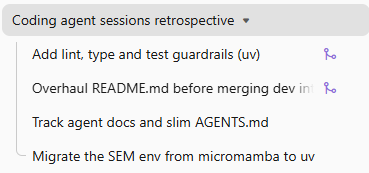
\includegraphics[height=23.4mm]{assets/screens/claude-app-forks.png}};
    \begin{scope}[shift={(shot.south west)},x={($(shot.south east)-(shot.south west)$)},
        y={($(shot.north west)-(shot.south west)$)}]
      \node[number mark] at (0.813,0.879) {1};
      \node[number mark] at (0.043,0.387) {2};
      \node[number mark] at (0.954,0.682) {3};
    \end{scope}
    \foreach \t [count=\k] in {one session,{its forks, one per task},pull request merged} {
      \node[number mark] at (56.4,-33.6-\k*6.6+6.6) {\k};
      \node[key] at (59.6,-33.6-\k*6.6+6.6) {\t};
    }
    \fill[termbg,rounded corners=1.2mm] (100,-31.4) rectangle (144,-45.6);
    \foreach \c [count=\i] in {termdot1,termdot2,termdot3} \fill[\c] (100.4+\i*2.3,-34) circle (0.7);
    \node[inner sep=0pt,font=\ttfamily\fontsize{7}{8}\selectfont,text=termdim] at (124.6,-34)
      {second terminal};
    \draw[white!18!termbg,line width=0.4pt] (100,-36.6) -- (144,-36.6);
    \node[mono,text=termfg] at (102.4,-39.6) {\textcolor{termgreen}{\$} claude -c --fork-session};
    \node[mono,text=termfg] at (102.4,-43) {> work in a worktree};
    \node[anchor=north west,inner sep=0pt,font=\scriptsize,text=udsgrey] at (100,-47.4)
      {forks the latest session in this folder};
  \end{tikzpicture}
  \note{\textbf{24:00--24:50}\par
    A tip from daily use: a session often turns into more than one task.\par
    Fork it with slash fork rather than start again: each fork keeps the whole conversation, the
      plan and the decisions included.\par
    Then ask each fork to work in a worktree; Claude Code creates one under .claude/worktrees and
      moves the session into it.\par
    Until then both forks work in the same folder, and their edits can collide.\par
    In the app the forks sit under their session in the sidebar: here four tasks that came out of
      one session, each in its own worktree; purple marks a merged pull request.\par
    In a terminal, slash fork copies the conversation into a new session and keeps you in this
      one; from a second terminal, claude with continue and fork-session copies the latest session
      of the folder.}
\end{frame}

\section[Tests first]{Tests first}
\sectionframe{06}{Tests first}
  {How does a test written before the code keep an agent on track?}
  {\faCheckDouble}

% ---------------------------------------------------------------- the loop
\begin{frame}[source={Beck (2002), Test-Driven Development: By Example}]{Test-Driven Development (TDD)}
  \begin{tikzpicture}[x=1mm,y=1mm,
      phase/.style={box,text width=28mm,minimum height=13mm,font=\footnotesize,line width=0.8pt},
      gain/.style={inner sep=0pt,font=\footnotesize,text=udsdark,align=left},
      tick/.style={inner sep=0pt,font=\footnotesize,anchor=base east}]
    \useasboundingbox (0,-1.36) rectangle (144,-55);
    \node[phase,draw=udsred,fill=redtint] (red) at (72,-8)
      {{\color{udsred}\bfseries\small RED}\\[0.4mm] write a failing test for one behaviour};
    \node[phase,draw=testgreen,fill=greentint] (green) at (96,-40)
      {{\color{testgreen}\bfseries\small GREEN}\\[0.4mm] write just enough code to pass it};
    \node[phase,draw=udsblue,fill=bluetint] (ref) at (48,-40)
      {{\color{udsblue}\bfseries\small REFACTOR}\\[0.4mm] tidy the code; every test stays green};
    \draw[flow] (red.east) to[bend left=35] (green.north);
    \draw[flow] (green.west) -- (ref.east);
    \draw[flow] (ref.north) to[bend left=35] (red.west);
    \node[lbl,align=center] at (72,-27) {one behaviour\\per cycle};
    % what each step gives us; each tick sits on its gain's first baseline (with a text width,
    % a node's base is its first line); the two gains of RED start at x = 98, clear of the arrow
    % from RED to GREEN
    \node[gain,anchor=west] (g1) at (98,-5.2) {the requirement, written first};
    \node[gain,anchor=west] (g2) at (98,-10.8) {proof that the test can fail};
    \node[gain,anchor=west,text width=20mm] (g3) at (118.4,-40) {small steps,\\easy to review};
    \node[gain,anchor=west,text width=22mm] (g4) at (8,-40) {a regression net\\for later changes};
    \foreach \g/\c in {g1/udsred,g2/udsred,g3/testgreen,g4/udsblue}
      \node[tick,text=\c] at ([xshift=-1.4mm]\g.base west) {\faCheck};
    \node[gain,anchor=base] (g5) at (74,-53.4) {tests call clear interfaces: the seams};
    \node[tick,text=udsdark] at ([xshift=-1.4mm]g5.base west) {\faCheck};
  \end{tikzpicture}
  \note{\textbf{25:00--26:00}\par
    Test-driven development in Kent Beck's formulation is a short loop.\par
    Red: write a test for one behaviour and watch it fail.\par
    Green: write just enough code to make it pass.\par
    Refactor: tidy the code while all tests stay green.\par
    Then the next behaviour.\par
    What we get: the requirement written down as a test before the code exists, proof that each
      test can fail, small steps, a regression net, and pressure towards clear interfaces, the
      seams where tests observe behaviour.}
\end{frame}

% ------------------------------------------------------- why for an agent
\begin{frame}[source={Anthropic (2026), Claude Code best practices · Mathews \& Nagappan (2024), ASE ’24}]{Why tests first help an agent}
  \begin{tikzpicture}[x=1mm,y=1mm,
      node2/.style={box,minimum height=9mm,inner sep=1.6mm},
      item/.style={anchor=base west,inner sep=0pt,font=\footnotesize,text=udsdark},
      head/.style={anchor=base west,inner sep=0pt,font=\footnotesize\bfseries}]
    \useasboundingbox (0,0) rectangle (144,-54);
    % the agent edits the code and runs the tests
    \node[node2,artifact,font=\ttfamily\footnotesize\bfseries,minimum width=20mm] (src) at (12,-8) {src/};
    \node[node2,agent,font=\footnotesize\bfseries,minimum width=26mm] (ag) at (62,-8) {\faRobot\enspace agent};
    \node[node2,artifact,draw=testgreen,fill=greentint,font=\ttfamily\footnotesize\bfseries,minimum width=20mm]
      (tst) at (114,-8) {tests/};
    \draw[flow] (ag.west) -- node[lbl,above] {edits} (src.east);
    \draw[flow] (ag.east) -- node[lbl,above] {runs} (tst.west);
    \node[anchor=south,inner sep=0pt,font=\scriptsize,text=testgreen] at ([yshift=1mm]tst.north)
      {\faLock\enspace approved and committed first};
    % pass or fail comes back: the signal
    \draw[flow,draw=testgreen,line width=0.8pt] (tst.south) to[out=-90,in=-90,looseness=0.55]
      node[pos=0.5,below,inner sep=0.8mm,font=\scriptsize\bfseries,text=testgreen] {pass or fail} (ag.south);
    % what the signal gives the agent
    \node[head,text=testgreen] at (0,-28.4) {what it gives the agent};
    \foreach \t [count=\i] in {a check it runs itself,{the intent, fixed first},one small goal per cycle,
        earlier decisions still enforced}
      \node[item] at (0,-28.4-\i*4.7) {\textcolor{testgreen}{\faCheck}\enspace\t};
    % how it gets gamed: aimed at the tests, and what catches it
    \node[head,text=udsred] (gamed) at (70,-28.4) {how it gets gamed};
    \foreach \t [count=\i] in {tests edited or skipped,expected values copied from the code,
        a mock that replaces the logic,tests fitted after the code}
      \node[item] at (70,-28.4-\i*4.7) {\textcolor{udsred}{\faTimes}\enspace\t};
    \draw[udsred,line width=0.6pt,dashed,-{Stealth[length=1.7mm,width=1.3mm]}]
      ([xshift=1.5mm]gamed.east) to[out=0,in=-90] (121,-12.6);
    \node[item,text=udsblue] at (70,-53)
      {caught by: test diffs reviewed first · you rerun every test};
  \end{tikzpicture}
  \note{\textbf{26:00--27:00}\par
    Anthropic's guidance for Claude Code puts it plainly: without a check it can run, an agent
      stops when the work looks done.\par
    A failing test turns done into a signal the agent reads and iterates on.\par
    Written first, from the spec, the test records intent instead of mirroring the
      implementation, and the suite keeps earlier decisions enforced in later sessions.\par
    The failure modes are real: agents weaken, skip or edit tests, recompute expected values the
      way the code does, or replace the logic under test with a mock, a stand-in that returns
      whatever the test expects.\par
    Hence our guardrails: read the changes to the tests first, and rerun every test yourself
      rather than trust the agent's report.\par
    A benchmark study found that giving the model the tests with the task solved more problems;
      that is evidence for code generation, not for research code.}
\end{frame}

\section[Workflow]{Skills and an end-to-end workflow}
\sectionframe{07}{Skills and an end-to-end workflow}
  {How does a request become a reviewed change?}
  {\faProjectDiagram}

% ------------------------------------------------------------ what a skill is
% a lab protocol beside a skill file, row for row: what it is called, when to use it, the steps
\begin{frame}[source={Pocock (2026), mattpocock/skills v1.3.1: tdd · agentskills.io, Specification}]{A skill: a lab protocol for the agent}
  \begin{tikzpicture}[x=1mm,y=1mm,
      head/.style={anchor=north west,inner sep=0pt,font=\small\bfseries,text=udsdark},
      prot/.style={anchor=base west,inner sep=0pt,font=\footnotesize,text=udsdark},
      code/.style={anchor=base west,inner sep=0pt,font=\ttfamily\fontsize{7.2}{8.4}\selectfont,text=udsdark},
      num/.style={circle,fill=udsblue,text=white,inner sep=0pt,minimum size=3.6mm,
        font=\fontsize{7}{7}\selectfont\bfseries},
      pair/.style={udsgreymid,line width=0.5pt,dash pattern=on 1pt off 1pt},
      key/.style={fill=white,inner xsep=0.8mm,inner ysep=0.3mm,font=\scriptsize,text=udsgrey},
      say/.style={anchor=north west,inner sep=0pt,font=\scriptsize,text=udsdark}]
    \useasboundingbox (0,0) rectangle (144,-55);
    \node[head] at (0,0) {In the lab\enspace{\mdseries\color{udsgrey}a protocol}};
    \node[head] at (76,0) {In the repository\enspace{\mdseries\color{udsgrey}a skill}};
    % the protocol: a sheet on a clipboard
    \draw[udsgreylight,fill=white,line width=0.5pt,rounded corners=1.2mm] (0,-5.6) rectangle (62,-43.6);
    \fill[udsgreymid,rounded corners=0.8mm] (24,-4.3) rectangle (38,-7.1);
    \node[prot,font=\footnotesize\bfseries] at (3,-14.6) {Sample preparation};
    \node[prot,text=udsgrey] at (3,-18.6) {Use when: a specimen goes to the SEM.};
    \foreach \t [count=\i] in {Grind.,Polish.,Etch.,Check under the light microscope.} {
      \pgfmathsetmacro\y{-29-(\i-1)*4}
      \node[num] at (4.8,\y+0.95) {\i};
      \node[prot] at (8.4,\y) {\t};
    }
    % the skill: its SKILL.md in a file window, as on the slides of section 3
    \node[anchor=north west,inner xsep=1.8mm,inner ysep=0.8mm,text height=1.9mm,text depth=0.6mm,
      font=\ttfamily\fontsize{7}{8}\selectfont,text=udsdark] (tab) at (76,-5.6)
      {\textcolor{udsblue}{\faIcon[regular]{file-alt}}\enspace tdd/SKILL.md\enspace
       \textcolor{udsgreymid}{\sffamily\scriptsize shortened}};
    \begin{scope}
      \clip[rounded corners=1.2mm] (76,-5.6) rectangle (144,-43.6);
      \fill[darktint] (tab.north east) rectangle (144,-9.7);
      \draw[udsblue,line width=0.9pt] (tab.north west) -- (tab.north east);
    \end{scope}
    \draw[udsgreylight,line width=0.5pt,rounded corners=1.2mm] (76,-5.6) rectangle (144,-43.6);
    \node[code] at (78.8,-14.6) {name: tdd};
    \node[code] at (78.8,-18.6) {description: Test-driven development. Use when};
    \node[code] at (78.8,-21.6) {\phantom{xx}the user wants to build features or fix};
    \node[code] at (78.8,-24.6) {\phantom{xx}bugs test-first, ...};
    \foreach \t [count=\i] in {Agree the seams to test.,Write one failing test.,
        Write just enough code to pass.,Repeat for the next behaviour.}
      \node[code] at (78.8,{-29-(\i-1)*4}) {\i. \t};
    % what matches what, the word on its line
    \foreach \y/\k in {-13.7/name,-17.7/when,-34.6/steps} {
      \draw[pair] (63.2,\y) -- (74.8,\y);
      \node[key] at (69,\y) {\k};
    }
    \node[say] at (0,-44.8) {written once; everyone in the lab follows it};
    \node[say] at (76,-44.8) {written once; the agent follows it when needed};
    % when a skill is worth writing, in a strip like the one of slide 5, 2 mm below the captions
    \fill[bluetint] (0,-49.6) rectangle (144,-55);
    \fill[udsblue] (0,-49.6) rectangle (1.2,-55);
    \node[anchor=west,inner sep=0pt,font=\footnotesize,text=udsdark] at (3.6,-52.3)
      {\textcolor{udsblue}{\faClipboardList}\enspace one procedure per kind of task};
    \node[anchor=west,inner sep=0pt,font=\footnotesize,text=udsdark] at (74,-52.3)
      {\textcolor{udsblue}{\faRedo}\enspace worth writing when the task recurs};
  \end{tikzpicture}
  \note{\textbf{27:10--28:10}\par
    Section 3 gave the agent facts about the repository; a skill gives it a procedure.\par
    It works like a lab protocol: a name, when to use it, and the steps, written once and
      followed by whoever does the task.\par
    A skill is the same for an agent: a Markdown file, here a shortened version of Pocock's
      test-driven development skill.\par
    Without one, we type the same instructions into every prompt, a little differently each
      time.\par
    Written once, the procedure is kept with the project, reviewed like code and improved in one
      place.\par
    Worth it for a task that recurs; a one-off task needs only a good prompt.}
\end{frame}

% ------------------------------------------------------------ inside a skill
\begin{frame}[fragile,source={Pocock (2026), mattpocock/skills v1.3.1: tdd · agentskills.io, Specification · Anthropic (2026), Claude Code docs: Skills · OpenAI (2026), Build skills}]{A skill: procedures loaded when needed}
  \begin{columns}[T,onlytextwidth]
    \begin{column}{0.57\textwidth}
\begin{codefile}[basicstyle=\ttfamily\fontsize{7}{8.4}\selectfont]{tdd/SKILL.md\enspace\textcolor{udsgreymid}{\sffamily\scriptsize shortened}}
---
name: tdd
description: Test-driven development. Use when the user
  wants to build features or fix bugs test-first,
  mentions "red-green-refactor", or wants integration
  tests.
---
# Test-Driven Development
## What a good test is
Tests verify behavior through public interfaces, not
implementation details. ...
See [tests.md](tests.md) for examples and
[mocking.md](mocking.md) for mocking guidelines.
\end{codefile}
      % where the skill folders go, under the file and flush with it
      {\scriptsize\color{udsgrey}\textcolor{udsblue}{\faFolderOpen}\enspace\fn{.claude/skills/} (Claude Code),
       \fn{.agents/skills/} (Codex)\par}
    \end{column}
    \begin{column}{0.4\textwidth}
      % one bracket per part of the file, level with its lines; y = 0 is the top of the file window
      \begin{tikzpicture}[x=1mm,y=1mm,
          what/.style={anchor=west,inner sep=0pt,font=\footnotesize,text=udsdark,align=left,text width=52mm,
            execute at begin node={\hyphenpenalty=10000\raggedright}}]
        \useasboundingbox (0,0) rectangle (57.6,-54);
        \def\first{6.6}\def\pitch{2.952}% the first line's top below the window's top, and the line pitch
        \foreach \a/\b/\t in {1/7/{\textcolor{udsblue}{\bfseries from the start}, like \fn{AGENTS.md}\\
              the name and description of every skill},
            8/11/{\textbf{when it runs}\\ \fn{/tdd}, or a task that matches},
            12/13/{\textbf{when the steps need them}\\ \fn{tests.md}, \fn{mocking.md} in the same folder}} {
          \pgfmathsetmacro\ya{-\first-(\a-1)*\pitch-0.5}
          \pgfmathsetmacro\yb{-\first-\b*\pitch+0.5}
          \draw[udsgreymid,line width=0.6pt] (0,\ya) -- (1.4,\ya) -- (1.4,\yb) -- (0,\yb);
          \node[what] at (3.6,{(\ya+\yb)/2}) {\t};
        }
      \end{tikzpicture}
    \end{column}
  \end{columns}
  \note{\textbf{28:10--29:20}\par
    Technically, a skill is a folder with a SKILL.md file and, where needed, more files beside
      it.\par
    The file starts with a name and a description, which says what the skill is for and when to
      use it.\par
    At the start of a session the agent sees only these lines, for every installed skill, about a
      hundred tokens each, just as it always sees AGENTS.md.\par
    The rest of the file loads when the skill runs: when we type its name, here /tdd, or when the
      agent finds that a task matches the description.\par
    Files beside it, here examples of good tests and rules for mocks, are read only when the
      steps call for them; this is called progressive disclosure.\par
    Committed with the code, the skill reaches everyone who works in the repository.}
\end{frame}

% ------------------------------------------------------------ the collection
\begin{frame}[source={Pocock (2026), mattpocock/skills v1.3.1: README · github.com/mattpocock/skills, 20 Oct 2026}]{Matt Pocock's skills: an end-to-end workflow}
  \begin{columns}[T,onlytextwidth]
    \begin{column}{0.56\textwidth}
      % the repository's address, which the screenshot's crop leaves out, as a link
      {\footnotesize\href{https://github.com/mattpocock/skills}{\faGithub\enspace\underline{\fn{mattpocock/skills}}}\par}
      \vskip1.6mm
      \begin{tikzpicture}
        \node[anchor=south west,inner sep=0pt,draw=udsgreylight,line width=0.4pt] (img) at (0,0)
          {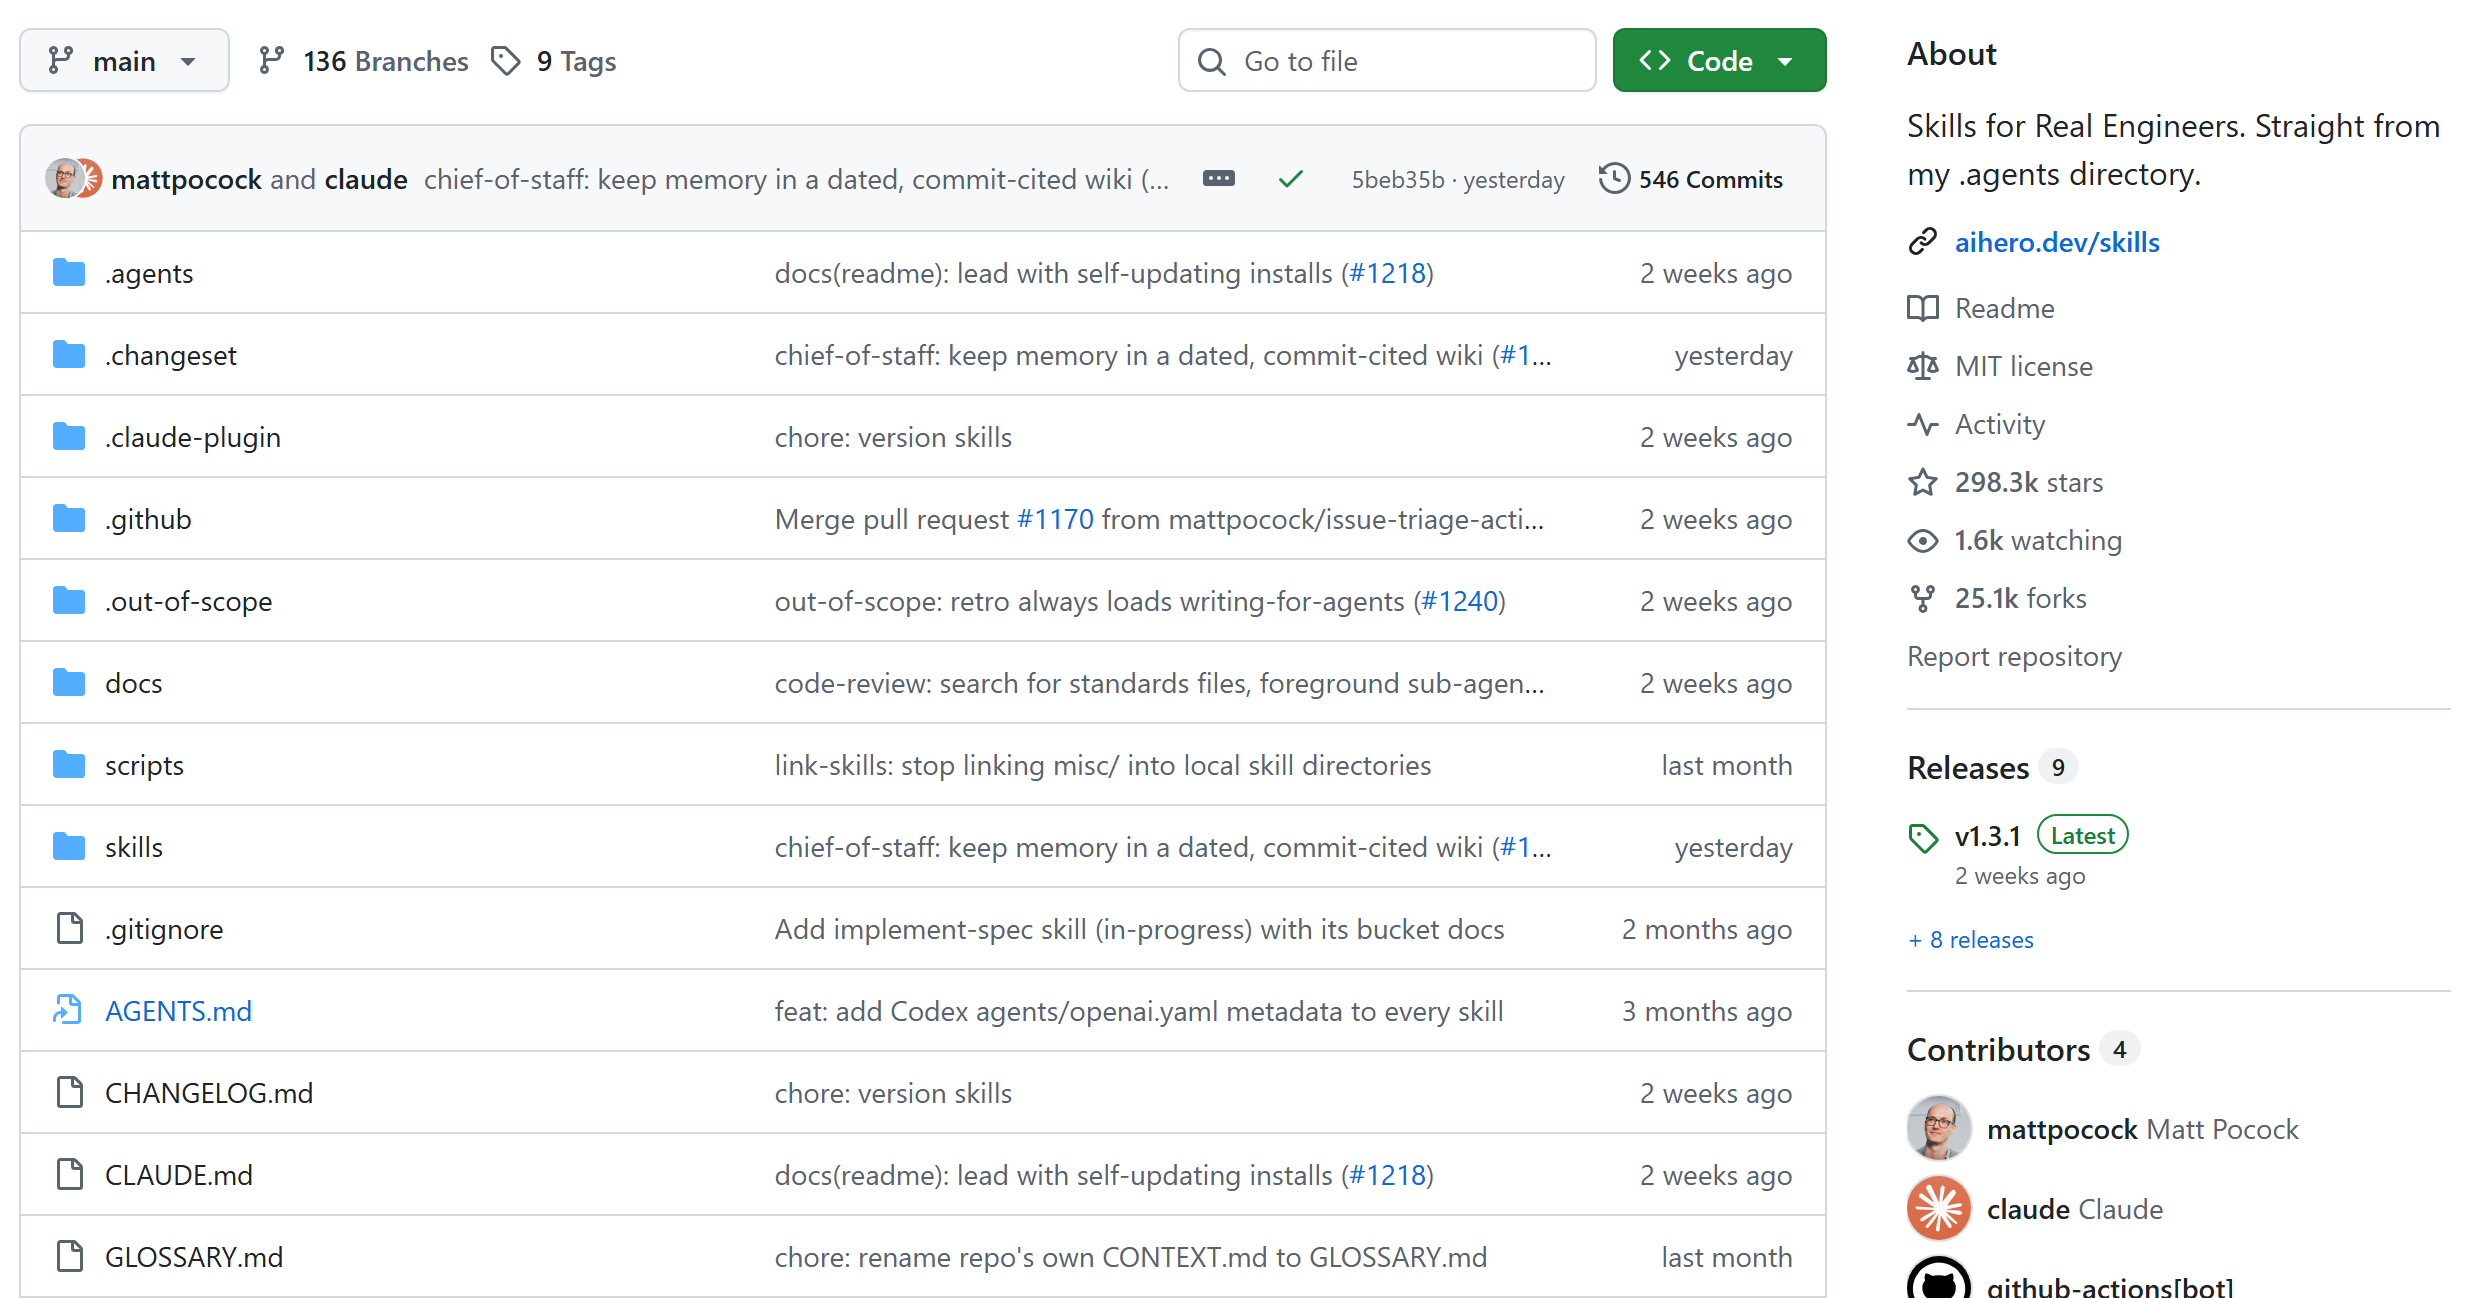
\includegraphics[width=\linewidth]{assets/screens/github-skills.png}};
        \begin{scope}[x={(img.south east)},y={(img.north west)},udsred,line width=1.1pt]
          \draw (0.014,0.320) rectangle (0.077,0.374);
          \draw (0.014,0.193) rectangle (0.109,0.247);
          \draw (0.014,0.005) rectangle (0.123,0.058);
          \draw (0.766,0.333) rectangle (0.871,0.386);
        \end{scope}
      \end{tikzpicture}
    \end{column}
    \begin{column}{0.41\textwidth}
      % two kinds of skill: the ones you type run a stage, and call the ones the agent may also pick
      \begin{tikzpicture}[x=1mm,y=1mm,
          kind/.style={anchor=north west,inner sep=0pt,font=\footnotesize\bfseries},
          chip/.style={anchor=west,minimum height=4.6mm,inner xsep=1mm,inner ysep=0pt,line width=0.5pt,
            font=\ttfamily\fontsize{7}{8}\selectfont,text=udsdark},
          you/.style={chip,draw=udsred,fill=redtint,minimum width=23.6mm},
          it/.style={chip,draw=udsblue,fill=bluetint,minimum width=22mm},
          call/.style={-{Stealth[length=1.5mm,width=1.1mm]},line width=0.5pt,draw=udsdark},
          say/.style={anchor=north west,inner sep=0pt,font=\scriptsize,text=udsgrey}]
        \useasboundingbox (0,0) rectangle (59,-54);
        \node[kind,text=udsred] at (0,0) {\faUser\enspace you type};
        \node[kind,text=udsblue] at (31,0) {\faRobot\enspace the agent may use};
        \foreach \s [count=\i from 0] in {/grill-with-docs,/to-spec,/to-tickets,/implement}
          \node[you] (u\i) at (0,{-7.6-\i*6.4}) {\s};
        \foreach \s [count=\i from 0] in {domain-modeling,codebase-design,tdd,code-review}
          \node[it] (m\i) at (31,{-7.6-\i*6.4}) {\s};
        % who calls whom, as the SKILL.md files say
        \draw[call] (u0.east) -- (m0.west);
        \draw[call] (u3.east) -- (m2.west);
        \draw[call] (u3.east) -- (m3.west);
        \draw[call] (m2.east) to[out=0,in=0,looseness=1.6] (m1.east);
        \node[say] at (0,-31.6) {each runs one stage};
        \node[say] at (31,-31.6) {rules and vocabulary};
        % installing: the files are copied into the project
        \fill[termbg,rounded corners=1mm] (0,-37) rectangle (57,-45.8);
        \foreach \c [count=\i] in {termdot1,termdot2,termdot3} \fill[\c] (\i*2.3,-39.2) circle (0.7);
        \node[inner sep=0pt,font=\ttfamily\fontsize{7}{8}\selectfont,text=termdim] at (28.5,-39.2) {install};
        \node[anchor=west,inner sep=0pt,font=\ttfamily\fontsize{7}{8}\selectfont,text=termfg] at (1.8,-43.4)
          {\textcolor{termgreen}{\$} npx skills@latest add mattpocock/skills};
        \node[say,text=udsred] at (0,-47.6) {\faExclamationTriangle\enspace read them first};
      \end{tikzpicture}
    \end{column}
  \end{columns}
  \note{\textbf{29:20--30:10}\par
    Our example is Matt Pocock's open-source collection on GitHub; the repository uses its own
      AGENTS.md and GLOSSARY.md.\par
    Its skills come in two kinds: the ones we type each run one stage of the work, and they call
      skills that the agent may also pick up by itself, which hold the rules.\par
    Grill-with-docs calls domain-modeling, implement calls tdd and code-review, and tdd looks up
      codebase-design for its vocabulary.\par
    The installer copies the files into the project; skills are instructions and scripts written
      by someone else, so read them before the agent uses them.}
\end{frame}

% ------------------------------------------------------- the books behind
% \bookcover{x}{colour}{title}{author}{year}: a book seen from the front, 22 x 27 mm, its top-left
% corner at (x,0); the darker strip on the left is the spine
\newcommand\bookcover[5]{%
  \begin{scope}
    \clip[rounded corners=0.9mm] (#1,0) rectangle ++(22,-27);
    \fill[#2] (#1,0) rectangle ++(22,-27);
    \fill[black,opacity=0.22] (#1,0) rectangle ++(1.9,-27);
  \end{scope}
  \node[anchor=north west,inner sep=0pt,text width=17.6mm,align=left,font=\scriptsize\bfseries,
    text=white,execute at begin node={\hyphenpenalty=10000\raggedright}] at (#1+3,-2.6) {#3};
  \node[anchor=south west,inner sep=0pt,text width=17.6mm,align=left,font=\scriptsize,
    text=white!80!#2] at (#1+3,-2.4-22.2) {#4\\#5};}
\begin{frame}[source={Hunt \& Thomas (1999) · Beck (1999; 2002) · Fowler (1999) · Evans (2003) · Ousterhout (2018) · Pocock (2026), mattpocock/skills v1.3.1: README, code-review, codebase-design}]{Classic practice, adapted for agents}
  % each book, the idea the skills take from it, and the skills that carry it
  \begin{tikzpicture}[x=1mm,y=1mm,
      idea/.style={anchor=north west,inner sep=0pt,text width=22mm,align=left,font=\scriptsize,
        text=udsdark,execute at begin node={\hyphenpenalty=10000\raggedright}},
      sk/.style={spec skill},
      fl/.style={spec chip}]
    \useasboundingbox (0,0) rectangle (144,-54);
    \bookcover{0}{udsdark}{The Pragmatic Programmer}{Andrew Hunt,\\David Thomas}{1999}
    \bookcover{24.4}{udsblue}{Extreme Programming Explained}{Kent Beck}{1999}
    \bookcover{48.8}{udsdark}{Refactoring}{Martin Fowler}{1999}
    \bookcover{73.2}{testgreen}{Test-Driven Development: By Example}{Kent Beck}{2002}
    \bookcover{97.6}{udsblue}{Domain-Driven Design}{Eric Evans}{2003}
    \bookcover{122}{udsdark}{A Philosophy of Software Design}{John\\Ousterhout}{2018}
    \foreach \x/\t in {0/{no one knows exactly what they want},24.4/{user stories; invest in the design every day},
        48.8/{code smells},73.2/{red, green, refactor},97.6/{a ubiquitous language},122/{deep modules}}
      \node[idea] at (\x,-29.4) {\t};
    \node[sk] at (0,-39.6) {/grill-with-docs};
    \node[sk] at (24.4,-39.6) {/to-spec};
    \node[sk] at (48.8,-39.6) {/code-review};
    \node[sk] at (73.2,-39.6) {/tdd};
    \node[fl] at (97.6,-39.6) {GLOSSARY.md};
    \node[sk] at (97.6,-45.2) {/domain-modeling};
    \node[sk] at (122,-39.6) {/codebase-design};
  \end{tikzpicture}
  \note{\textbf{30:10--31:20}\par
    None of this is new: Pocock's README says the skills rest on decades of engineering
      experience, and quotes the books.\par
    The Pragmatic Programmer: no one knows exactly what they want, so the agent asks before it
      builds; its tracer bullets return as the vertical slices of to-tickets.\par
    Kent Beck's Extreme Programming brought the user stories that to-spec writes into every spec,
      and the advice to invest in the design every day.\par
    Fowler's Refactoring catalogues code smells, which code-review looks for in every diff.\par
    Beck's red, green, refactor loop, the subject of section 6, is the tdd skill.\par
    Evans: one ubiquitous language for people and code, our glossary; Ousterhout: deep modules,
      much behaviour behind a small interface.\par
    What is new is the reader: the model has read these books, so a term such as tracer bullets
      or red and green brings the whole practice into a skill in a few words.}
\end{frame}

% Pocock's README, section "Why These Skills Exist", word for word (mattpocock/skills, MIT licence;
% the same on main on 3 November 2026 as in v1.3.1), with its links and the aside on the commit of its example glossary dropped: notes pages of their
% own, outside the frame, so they follow slide 29's notes page and stay out of the audience PDF. A
% note outside a frame does not get the theme's note style, so each one sets it first.
\note{\parindent=0pt\parskip=1.1mm\raggedright\footnotesize
  \textbf{Slide 29, continued (1 of 5): Pocock's README, ``Why These Skills Exist''}\par
  I built these skills as a way to fix common failure modes I see with Claude Code, Codex, and other
    coding agents.\par
  \textbf{\#1: The Agent Didn't Do What I Want}\par
  \emph{``No-one knows exactly what they want''}\enspace--- David Thomas \& Andrew Hunt, The Pragmatic
    Programmer\par
  \textbf{The Problem}. The most common failure mode in software development is misalignment. You think
    the dev knows what you want. Then you see what they've built - and you realize it didn't understand
    you at all.\par
  This is just the same in the AI age. There is a communication gap between you and the agent. The fix
    for this is a \textbf{grilling session} - getting the agent to ask you detailed questions about what
    you're building.\par
  \textbf{The Fix} is to use: \fn{/grill-me} - for non-code uses; \fn{/grill-with-docs} - same as
    \fn{/grill-me}, but adds more goodies (see below).\par
  These are my most popular skills. They help you align with the agent before you get started, and
    think deeply about the change you're making. Use them \emph{every} time you want to make a
    change.}
\note{\parindent=0pt\parskip=1.1mm\raggedright\footnotesize
  \textbf{Slide 29, continued (2 of 5)}\par
  \textbf{\#2: The Agent Is Way Too Verbose}\par
  \emph{``With a ubiquitous language, conversations among developers and expressions of the code are
    all derived from the same domain model.''}\enspace--- Eric Evans, Domain-Driven-Design\par
  \textbf{The Problem}: At the start of a project, devs and the people they're building the software
    for (the domain experts) are usually speaking different languages.\par
  I felt the same tension with my agents. Agents are usually dropped into a project and asked to figure
    out the jargon as they go. So they use 20 words where 1 will do.\par
  \textbf{The Fix} for this is a shared language. It's a document that helps agents decode the jargon
    used in the project.\par
  Example: here's an example glossary, from my \fn{course-video-manager} repo. Which one is easier to
    read? \textbf{BEFORE}: ``There's a problem when a lesson inside a section of a course is made `real'
    (i.e.\ given a spot in the file system)''. \textbf{AFTER}: ``There's a problem with the
    materialization cascade''. This concision pays off session after session.}
\note{\parindent=0pt\parskip=1.1mm\raggedright\footnotesize
  \textbf{Slide 29, continued (3 of 5)}\par
  \textbf{\#2, continued}\par
  This is built into \fn{/grill-with-docs}. It's a grilling session, but that helps you build a shared
    language with the AI, and document hard-to-explain decisions in ADR's.\par
  It's hard to explain how powerful this is. It might be the single coolest technique in this repo.
    Try it, and see.\par
  Tip: a shared language has many other benefits than reducing verbosity: \textbf{variables, functions
    and files are named consistently}, using the shared language; as a result, the \textbf{codebase is
    easier to navigate} for the agent; the agent also \textbf{spends fewer tokens on thinking}, because
    it has access to a more concise language.}
\note{\parindent=0pt\parskip=1.1mm\raggedright\footnotesize
  \textbf{Slide 29, continued (4 of 5)}\par
  \textbf{\#3: The Code Doesn't Work}\par
  \emph{``Always take small, deliberate steps. The rate of feedback is your speed limit. Never take on a
    task that's too big.''}\enspace--- David Thomas \& Andrew Hunt, The Pragmatic Programmer\par
  \textbf{The Problem}: Let's say that you and the agent are aligned on what to build. What happens when
    the agent \emph{still} produces crap?\par
  It's time to look at your feedback loops. Without feedback on how the code it produces actually runs,
    the agent will be flying blind.\par
  \textbf{The Fix}: You need the usual tranche of feedback loops: static types, browser access, and
    automated tests.\par
  For automated tests, a red-green-refactor loop is critical. This is where the agent writes a failing
    test first, then fixes the test. This helps give the agent a consistent level of feedback that
    results in far better code.\par
  I've built a \textbf{\fn{/tdd} skill} you can slot into any project. It encourages red-green-refactor
    and gives the agent plenty of guidance on what makes good and bad tests.\par
  For debugging, I've also built a \textbf{\fn{/diagnosing-bugs}} skill that wraps best debugging
    practices into a disciplined loop, gated phase by phase.}
\note{\parindent=0pt\parskip=1.1mm\raggedright\footnotesize
  \textbf{Slide 29, continued (5 of 5)}\par
  \textbf{\#4: We Built A Ball Of Mud}\par
  \emph{``Invest in the design of the system \emph{every day}.''}\enspace--- Kent Beck, Extreme Programming
    Explained\par
  \emph{``The best modules are deep. They allow a lot of functionality to be accessed through a simple
    interface.''}\enspace--- John Ousterhout, A Philosophy Of Software Design\par
  \textbf{The Problem}: Most apps built with agents are complex and hard to change. Because agents can
    radically speed up coding, they also accelerate software entropy. Codebases get more complex at an
    unprecedented rate.\par
  \textbf{The Fix} for this is a radical new approach to AI-powered development: caring about the design
    of the code.\par
  This is built in to every layer of these skills: \fn{/to-spec} quizzes you about which modules you're
    touching before creating a spec.\par
  And crucially, \fn{/improve-codebase-architecture} surveys a codebase for deepening opportunities and
    hands you the candidates. I recommend running it on your codebase once every few days. It is a
    survey, not a rescue: on a genuinely old codebase it will find real candidates, but it won't
    untangle the mud for you.\par
  \textbf{Summary}: Software engineering fundamentals matter more than ever. These skills are my best
    effort at condensing these fundamentals into repeatable practices, to help you ship the best apps of
    your career. Enjoy.}

% ------------------------------------------------------------ flow diagram
\begin{frame}[source={Pocock (2026), mattpocock/skills v1.3.1}]{Pocock's flow: who does what}
  \begin{tikzpicture}[x=1mm,y=1mm,
      cell/.style={minimum width=24.4mm,text width=23.2mm,inner sep=0.6mm,align=center,
        execute at begin node={\hyphenpenalty=10000}},
      hcell/.style={cell,human,minimum height=9.6mm,font=\fontsize{7}{8}\selectfont},
      acell/.style={cell,agent,minimum height=17mm,font=\fontsize{7}{8}\selectfont},
      fcell/.style={cell,artifact,minimum height=7.6mm,font=\ttfamily\fontsize{7}{8}\selectfont},
      lane/.style={font=\fontsize{7}{8}\selectfont\bfseries,rotate=90,anchor=center,inner sep=0pt}]
    \node[lane,text=udsred]  at (3,-4.8)  {PERSON};
    \node[lane,text=udsblue] at (3,-23.5) {AGENT};
    \node[lane,text=udsdark] at (3,-39)   {OUTPUT};
    \foreach \skill/\act/\who/\res [count=\k from 0] in {
        grill-with-docs/{questions in rounds; updates the glossary}/{answer; settle the open points}/{GLOSSARY.md, ADR draft},
        to-spec/{writes the spec from the conversation}/{approve scope and acceptance}/{spec (file or issue)},
        to-tickets/{vertical slices, in order}/{approve slices and order}/{ticket files},
        implement/{drives /tdd at the agreed seams; runs the review; commits}/{confirm test seams; rerun the tests}/{code + tests, one commit},
        code-review/{standards and spec, in parallel; proposes refactoring}/{judge findings; review the science}/{report (in session)}} {
      \pgfmathsetmacro\x{20+\k*27.6}
      \node[hcell] (h\k) at (\x,-4.8) {\who};
      \node[acell] (a\k) at (\x,-23.5) {{\ttfamily\bfseries/\skill}\\[0.3mm]\act};
      \node[fcell] (f\k) at (\x,-39) {\res};
      % two-way: the person both steers the stage and decides on its output
      \draw[flow,{Stealth[length=1.7mm,width=1.3mm]}-{Stealth[length=1.7mm,width=1.3mm]},draw=udsred]
        (h\k.south) -- (a\k.north);
      \draw[flow] (a\k.south) -- (f\k.north);
    }
    \foreach \k [evaluate=\k as \n using int(\k+1)] in {0,...,3} \draw[flow,draw=udsblue] (a\k.east) -- (a\n.west);
    \node[artifact,anchor=north west,minimum width=134.6mm,minimum height=5mm,font=\scriptsize,inner sep=0.6mm]
      (ctx) at (7.8,-45.4) {read along the way:\enspace \texttt{AGENTS.md}\enspace\textperiodcentered\enspace
      \texttt{GLOSSARY.md}\enspace\textperiodcentered\enspace\texttt{docs/adr/}\enspace\textperiodcentered\enspace
      \texttt{CODING\_STANDARDS.md} (review)\enspace\textperiodcentered\enspace tests};
    \foreach \a/\b/\t in {7.8/87.4/{one session: clarify, specify, slice},
                          90.6/142.4/{a fresh session per ticket}} {
      \draw[udsgreymid,line width=0.5pt] (\a,-52.5) -- ++(0,-1.2) -- (\b,-53.7) -- ++(0,1.2);
      \node[lbl,anchor=north] at ({(\a+\b)/2},-54.1) {\t};
    }
  \end{tikzpicture}
  \note{\textbf{31:20--32:30}\par
    The main flow as the author documents it: clarify with grill-with-docs, write the spec, cut
      tickets, implement each ticket.\par
    In today's terms this is spec-driven development: an approved spec before any code, then each
      ticket built test-first.\par
    Tickets are vertical slices: each a thin path through the whole program, from the command
      line to the output, usable on its own.\par
    Implement drives the tdd skill at the test seams agreed in the spec, the public functions
      and command-line options that the tests call; then it runs code-review and commits.\par
    Code-review checks the repository's coding standards and the spec, and is where refactoring
      is proposed.\par
    Red marks the decisions that stay with us at every stage.\par
    The author's context advice: one session from clarification to tickets, then a fresh session
      per ticket that starts from the written ticket.}
\end{frame}

% ---------------------------------------------------- a grilling session
% \sessiondot{n}: the theme's \numbermark, 3.6 mm across; \sessionmark{n} is the same without height, so a
% marker on a session line does not move the lines around it
\newcommand\sessiondot[1]{\tikz[baseline=-0.75ex]\node[circle,fill=udsred,text=white,inner sep=0pt,
  minimum size=3.6mm,font=\sffamily\fontsize{7}{7}\selectfont\bfseries] {#1};}
\newcommand\sessionmark[1]{\smash{\sessiondot{#1}}}
% \sessionarrow{text}: a session line, then an arrow from its end across the column gap to the
% window in the right column; drawn inside the frame, so the notes thumbnail shows it too. The
% terminal's text sits 3.2 mm inside its right edge (1 mm box separation plus 2.2 mm padding).
\newcommand\sessionarrow[1]{%
  \setbox0\hbox{\setbox2\hbox{x}\spaceskip=\wd2 #1}\copy0
  \edef\sessionarrowend{\the\dimexpr\linewidth+3.2mm+\colgap-\wd0+0.1mm\relax}%
  \tikz[overlay,baseline=0pt]\draw[udsred,line width=0.8pt,-{Stealth[length=2mm,width=1.6mm]}]
    (1.4mm,0.9mm) -- (\sessionarrowend,0.9mm);}
\begin{frame}[fragile,source={Pocock (2026), mattpocock/skills v1.3.1: grill-with-docs, grilling, domain-modeling}]{A \texttt{/grill-with-docs} session}
  % the gap between the columns, which the glossary arrow crosses
  \edef\colgap{\the\dimexpr0.03\textwidth\relax}
  \begin{columns}[T,onlytextwidth]
    \begin{column}{0.61\textwidth}
\begin{terminal}[basicstyle=\ttfamily\fontsize{7}{8}\selectfont]{example session}
> /grill-with-docs Add validation folds by specimen to the
  training CLI, as decided in ADR-0003.
§\textcolor{termred}{\smash{\faQuestionCircle}}§ §\textbf{Q1 Default number of folds}§: the manifest lists §\sessionmark{1}§
  three specimens. One fold per specimen?
§\textcolor{termblue}{\smash{\faArrowRight}}§ Yes: k = number of specimens; --folds can lower it. §\sessionmark{2}§

§\textcolor{termred}{\smash{\faQuestionCircle}}§ §\textbf{Q2 What validation claims}§: each specimen is the only
  one of its material state, a term GLOSSARY.md lacks.
  Report folds as unseen material states, and add it?
§\textcolor{termblue}{\smash{\faArrowRight}}§ Yes.

§\textcolor{termred}{\smash{\faQuestionCircle}}§ §\textbf{Q3 Rows without specimen\_id}§: stop with a ValueError,
  as CODING_STANDARDS.md asks?
§\textcolor{termblue}{\smash{\faArrowRight}}§ Yes, and name the rows in the message.
> yes to all
§\sessionarrow{Updated GLOSSARY.md: Material state.}§
No ADR: the number of folds is easy to change later. §\sessionmark{3}§
\end{terminal}
    \end{column}
    \begin{column}{0.36\textwidth}
      % the legend on top; the glossary window at the bottom, level with the line that updates it
      \begin{minipage}[t][58mm][t]{\linewidth}
        \footnotesize
        \begin{tabular}{@{}c@{\enspace}l@{}}
          \sessiondot{1} & a fact the agent looked up\\[1.4mm]
          \sessiondot{2} & a recommended answer\\[1.4mm]
          \sessiondot{3} & an ADR only if hard to reverse\\
        \end{tabular}
        \vfill
\begin{codefile}[basicstyle=\ttfamily\fontsize{7}{8}\selectfont]{GLOSSARY.md\enspace\textcolor{udsgreymid}{new entry}}
Material state: the processing
  condition of a specimen (AsCast,
  Q980_0h_WC, Q980_9h_AC); here,
  one specimen per state.
\end{codefile}
        \vspace{-2.2mm}% the box's own skip below it, so its bottom meets the terminal's
      \end{minipage}
    \end{column}
  \end{columns}
  \note{\textbf{32:30--33:50}\par
    What grilling looks like on our request; the session is abridged and written for our example
      in the format of Pocock's skills.\par
    Each round asks every question that can be asked now, numbered, each with a recommended
      answer (2), worded so that yes accepts it.\par
    The agent looks up facts itself, here the number of specimens in the manifest (1), and
      leaves the decisions to us.\par
    When a term settles, it goes into the glossary at once (the arrow); here the session finds
      that every specimen is also the only one of its material state, which matters for what
      validation can claim.\par
    It offers an ADR only when a decision is hard to reverse, surprising and a real trade-off,
      so the number of folds gets none (3).\par
    Pocock's video of July 2026 shows a full session on his own project.}
\end{frame}

% ------------------------------------------------------------- walkthrough
% \stagefile{node}{x centre}{y top}{tab}{body}: a small file window under a stage, drawn as the
% codefile box is; (node) is its page and (nodet) its tab
\newcommand\stagefile[5]{%
  \node[anchor=north west,inner xsep=1mm,inner ysep=0.7mm,text height=1.9mm,text depth=0.5mm,
    font=\ttfamily\fontsize{7}{8}\selectfont,text=udsdark] (#1t) at (#2-12.2,#3)
    {\textcolor{udsblue}{\faIcon[regular]{file-alt}}\enspace#4};
  \node[anchor=north,minimum width=24.4mm,text width=22mm,inner xsep=1.2mm,inner ysep=1.3mm,
    align=left,font=\ttfamily\fontsize{7}{8.4}\selectfont,text=udsdark] (#1) at (#2,#3-4.2) {#5};
  \begin{scope}
    \clip[rounded corners=1mm] (#2-12.2,#3) rectangle ($(#1.south)+(12.2,0)$);
    \fill[darktint] (#1t.north east) rectangle (#2+12.2,#3-4.2);
    \draw[udsblue,line width=1.4pt] (#1t.north west) -- (#1t.north east);
  \end{scope}
  \draw[udsgreylight,line width=0.5pt,rounded corners=1mm] (#2-12.2,#3) rectangle ($(#1.south)+(12.2,0)$);}
\begin{frame}{The specimen split, stage by stage}
  \begin{tikzpicture}[x=1mm,y=1mm,
      stage/.style={agent,minimum width=24.4mm,minimum height=6.2mm,inner sep=0.6mm,
        font=\ttfamily\bfseries\fontsize{7}{8}\selectfont},
      ticket/.style={draw=udsgreylight,fill=white,line width=0.5pt,anchor=north,minimum width=24.4mm,
        text width=21.4mm,inner xsep=1.5mm,inner ysep=0.9mm,align=left,font=\scriptsize,text=udsdark,
        execute at begin node={\hyphenpenalty=10000\raggedright},
        path picture={\fill[udsdark] (path picture bounding box.north west) rectangle
          ([xshift=0.9mm]path picture bounding box.south west);}},
      say/.style={anchor=north,inner sep=0pt,font=\scriptsize,text=udsgrey,align=center,text width=25mm,
        execute at begin node={\hyphenpenalty=10000}},
      commit/.style={circle,draw=udsblue,fill=white,line width=0.9pt,minimum size=3mm,inner sep=0pt}]
    % an invisible copy of a lane label of "Pocock's flow: who does what" gives this picture the
    % same left edge, so the five columns sit exactly under those of that slide
    \node[font=\fontsize{7}{8}\selectfont\bfseries,rotate=90,anchor=center,inner sep=0pt,opacity=0]
      at (3,-4.8) {PERSON};
    % the short request starts the flow
    \fill[termbg,rounded corners=1mm] (7.8,0) rectangle (142.6,-6.4);
    \foreach \c [count=\i] in {termdot1,termdot2,termdot3} \fill[\c] (7.8+\i*2.3,-3.2) circle (0.7);
    \node[anchor=west,inner sep=0pt,font=\ttfamily\fontsize{7}{8}\selectfont,text=termfg] at (17,-3.2)
      {> Add validation folds by specimen to the training CLI, as decided in ADR-0003.};
    % the five stages, as on "Pocock's flow: who does what"
    \foreach \s [count=\k from 0] in {grill-with-docs,to-spec,to-tickets,implement,code-review}
      \node[stage] (s\k) at (20+\k*27.6,-13.6) {/\s};
    \draw[flow] (20,-6.4) -- (s0.north);
    \foreach \k [evaluate=\k as \n using int(\k+1)] in {0,...,3} \draw[flow,draw=udsblue] (s\k.east) -- (s\n.west);
    \foreach \k in {0,...,4} \draw[flow] (s\k.south) -- ++(0,-3.4);
    % 1: answers, and a new glossary term
    \stagefile{w0}{20}{-21.2}{GLOSSARY.md}{\textcolor{testgreen}{+}\,Material state}
    \node[say] at ([yshift=-1.4mm]w0.south) {Q1 to Q3 answered};
    % 2: the spec
    \stagefile{w1}{47.6}{-21.2}{spec.md}{\textcolor{udsblue}{\bfseries\#\# Decisions}\\
      \textcolor{udsblue}{\bfseries\#\# Test seams}\\ \textcolor{udsblue}{\bfseries\#\# Out of scope}}
    % 3: three vertical slices, each usable on its own
    \node[ticket] (t1) at (75.2,-21.2) {\textbf{T1}\enspace\fn{--split specimen}, end to end};
    \node[ticket] (t2) at ([yshift=-1.4mm]t1.south) {\textbf{T2}\enspace overlap guard and errors};
    \node[ticket] (t3) at ([yshift=-1.4mm]t2.south) {\textbf{T3}\enspace provenance in the fold file};
    % 4: one commit per ticket, each in a fresh session
    \draw[udsblue,line width=1pt] (95.4,-20.4) -- (95.4,-45.6);
    \foreach \t [count=\i from 0] in {T1,T2,T3} {
      \node[commit] (k\i) at (95.4,-24-\i*8.6) {};
      \node[anchor=west,inner sep=0pt,font=\scriptsize,text=udsdark] at ([xshift=1.4mm]k\i.east)
        {\textbf{\t}\enspace tests, code};
    }
    \node[say] at (102.8,-47.6) {a fresh session per ticket};
    % 5: the review report on two axes
    \stagefile{w4}{130.4}{-21.2}{report}{\fontsize{7}{8.4}\sffamily
      \textcolor{udsblue}{\faSearch}\enspace standards\\[0.4mm] \textcolor{udsblue}{\faSearch}\enspace spec}
    \node[say] at ([yshift=-1.4mm]w4.south) {findings for you to judge};
  \end{tikzpicture}
  \note{\textbf{33:50--35:00}\par
    The whole flow on our task, starting from the short request.\par
    Each stage leaves something we can open and check.\par
    Grilling settles what the repository leaves open: the default number of folds, and what
      validation is meant to show with only three specimens.\par
    The spec records the decisions and the test seams.\par
    Tickets are thin vertical slices, each usable on its own: first the whole path from the
      command line to a fold file, then the overlap guard and the error cases, then the
      provenance stored in the fold file.\par
    Each ticket is implemented test-first in a fresh session, and review checks the standards
      and the spec.}
\end{frame}

% ------------------------------------------------- /implement drives /tdd
\begin{frame}[source={Pocock (2026), mattpocock/skills v1.3.1: implement, tdd · aihero.dev/skills}]{How \texttt{/implement} uses \texttt{/tdd}}
  \begin{columns}[T,onlytextwidth]
    \begin{column}{0.48\textwidth}
      \begin{tikzpicture}[x=1mm,y=1mm,
          stp/.style={agent,text width=48mm,minimum height=6.6mm,align=left,font=\scriptsize,inner sep=1mm},
          num/.style={font=\scriptsize\bfseries,text=udsblue,anchor=east,inner sep=0.8mm}]
        \node[anchor=north west,inner sep=0pt,font=\footnotesize] at (0,0)
          {\fn{/implement}: one ticket, one fresh session};
        \node[stp,anchor=north west] (s1) at (6,-5)  {read the ticket};
        \node[stp,anchor=north west,draw=testgreen,fill=greentint,line width=0.8pt,minimum height=9mm] (s2) at (6,-14)
          {\fn{/tdd} at the agreed seams: one failing test, then just enough code to pass it};
        \node[stp,anchor=north west] (s3) at (6,-26) {typecheck; run single test files};
        \node[stp,anchor=north west] (s4) at (6,-35) {run the full suite once};
        \node[stp,anchor=north west] (s5) at (6,-44) {\fn{/code-review}, then commit};
        \foreach \i in {1,...,5} \node[num] at (s\i.west) {\i};
        \foreach \i [evaluate=\i as \j using int(\i+1)] in {1,...,4} \draw[flow] (s\i.south) -- (s\j.north);
        \draw[flow,draw=testgreen] ([yshift=-2.2mm]s2.east) -- ++(3.5,0) -- ++(0,4.4)
          node[midway,right,lbl,text=testgreen] {repeat} -- ++(-3.5,0);
      \end{tikzpicture}
    \end{column}
    \begin{column}{0.49\textwidth}
      \begin{gblock}[fontupper=\footnotesize]{Rules of the \texttt{/tdd} loop}
        \begin{itemize}\setlength\itemsep{0.5mm}
          \item seams agreed with you first
          \item one failing test, then minimal code
          \item one vertical slice per cycle
          \item tests only through public interfaces
          \item mocks only at system boundaries
          \item refactoring left to \fn{/code-review}
        \end{itemize}
      \end{gblock}
      {\footnotesize Known gaps: code written before its test; ticket left open; the run reviews its own
       work.\par}
    \end{column}
  \end{columns}
  \note{\textbf{35:00--36:10}\par
    In Pocock's skills, implement is the build step and you invoke it yourself, one ticket per
      fresh session.\par
    It reads the ticket, drives the tdd skill at the agreed seams one red-green slice at a time,
      typechecks and runs single test files as it goes, runs the full suite once at the end,
      calls code-review and commits.\par
    The tdd skill is a set of rules: seams agreed first, red before green, one vertical slice
      per cycle, tests through public interfaces, mocks only at system boundaries.\par
    The loop has no refactor step, because agents almost never do it; code-review
      proposes refactoring instead.\par
    The author's documentation lists the gaps: the agent sometimes writes code first, implement
      does not close the ticket, and the review inside the same run reviews its own work, so a
      fresh session makes a better reviewer.}
\end{frame}

% ---------------------------------------------------- when is it worth it
\begin{frame}[source={Pocock (2026), mattpocock/skills v1.3.1, ask-matt}]{When is the full flow worth it?}
  \centering
  \begin{tikzpicture}[x=1.55mm,y=1mm,pt/.style={circle,fill=udsdark,inner sep=0pt,minimum size=1.8mm}]
    \fill[bluetint] (0,0) rectangle (42,23);
    \fill[redtint] (42,23) rectangle (84,46);
    \draw[udsgreylight,line width=0.4pt] (42,0) -- (42,46) (0,23) -- (84,23);
    \draw[flow] (0,0) -- (86,0);
    \draw[flow] (0,0) -- (0,48);
    \node[lbl,anchor=north east,text=udsdark,font=\footnotesize] at (86,-0.8) {changes what a result means};
    \node[lbl,anchor=south,rotate=90,text=udsdark,font=\footnotesize] at (-0.8,24) {size and open questions};
    \node[lbl,anchor=south west,text=udsblue,font=\footnotesize\bfseries] at (1,1) {one prompt, review the diff};
    \node[lbl,anchor=north east,text=udsred,font=\footnotesize\bfseries] at (83,45) {grill, spec, tickets};
    \node[lbl,anchor=north west,text=udsdark,font=\footnotesize\bfseries] at (1,45) {slice it into tickets};
    \node[lbl,anchor=south east,text=udsdark,font=\footnotesize\bfseries] at (83,1) {write a short spec};
    \foreach \x/\y/\t in {7/9/fix a plot label, 14/16/add a CLI flag, 5/35/refactor the data loader,
        50/11/pixel-size units, 50/29/change the split unit, 60/38/new loss or metric} {
      \node[pt] (p) at (\x,\y) {};
      \node[lbl,anchor=west,text=udsdark,font=\scriptsize] at (p.east) {\t};
    }
  \end{tikzpicture}
  \note{\textbf{36:10--36:50}\par
    Not every change needs five stages.\par
    Two questions decide: how large or open is the change, and does it change what a result
      means?\par
    Small changes that leave results unchanged go straight to the agent; we still read the
      diff.\par
    A small change of meaning, such as pixel-size units, deserves a short spec.\par
    A large routine refactor benefits from tickets.\par
    The full flow earns its overhead when both hold, as for a new split unit, loss or
      metric.\par
    Pocock's own routing asks whether the build spans several sessions; the axis of meaning is
      ours.}
\end{frame}

\section[Adoption]{A realistic starting point}
\sectionframe{08}{A realistic starting point}
  {What should I change in my repository first?}
  {\faSeedling}

% ---------------------------------------------------- other skill packages
% \pkgcard{k}{owner}{repository}{head colour}{author}{what it is}{its steps}{its rule for tests}: card k
% (0 to 2), 46 mm wide and 3 mm apart; the green box at its foot holds the rule, level with the other
% cards' rules
\newcommand\pkgcard[8]{%
  \pgfmathsetmacro\pkx{#1*49}%
  \begin{scope}
    \clip[rounded corners=1.2mm] (\pkx,0) rectangle ++(46,-45.4);
    \fill[white] (\pkx,0) rectangle ++(46,-45.4);
    \fill[#4] (\pkx,0) rectangle ++(46,-9.2);
    \fill[greentint] (\pkx,-32.6) rectangle ++(46,-12.8);
    \fill[testgreen] (\pkx,-32.6) rectangle ++(1.2,-12.8);
  \end{scope}
  \draw[udsgreylight,line width=0.5pt,rounded corners=1.2mm] (\pkx,0) rectangle ++(46,-45.4);
  \node[anchor=north west,inner sep=0pt,font=\ttfamily\fontsize{7}{8.4}\selectfont,text=white!70!#4,
    align=left] at (\pkx+1.8,-1.5) {#2/\\\textcolor{white}{\bfseries #3}};
  \node[pkg who] at (\pkx+1.8,-10.8) {#5};
  \node[pkg what] at (\pkx+1.8,-14.8) {#6};
  \node[pkg text] at (\pkx+1.8,-22.6) {#7};
  \node[pkg text,text width=40.6mm] at (\pkx+3.6,-34.4) {\textcolor{testgreen}{\faCheck}\enspace #8};}
\begin{frame}[source={GitHub, 3 Nov 2026: obra/superpowers v7.0.1 · multica-ai/andrej-karpathy-skills · mattpocock/skills v1.3.1}]{Other skill packages}
  \begin{tikzpicture}[x=1mm,y=1mm,
      pkg who/.style={anchor=north west,inner sep=0pt,font=\scriptsize,text=udsgrey,text width=42.4mm,align=left},
      pkg what/.style={anchor=north west,inner sep=0pt,font=\footnotesize\bfseries,text=udsdark,
        text width=42.4mm,align=left,execute at begin node={\hyphenpenalty=10000\raggedright}},
      pkg text/.style={anchor=north west,inner sep=0pt,font=\scriptsize,text=udsdark,text width=42.4mm,
        align=left,execute at begin node={\hyphenpenalty=10000\raggedright}}]
    \useasboundingbox (0,0) rectangle (144,-54);
    \pkgcard{0}{mattpocock}{skills}{udsdark}{Matt Pocock}{small skills you combine}
      {grill, spec, tickets, implement, review}{\fn{/tdd}: red before green, at agreed seams}
    \pkgcard{1}{obra}{superpowers}{udsblue}{Jesse Vincent}{a whole method in 15 skills}
      {brainstorm, plan, execute, review, finish}{no production code without a failing test first}
    \pkgcard{2}{multica-ai}{andrej-karpathy-skills}{udsblue}{from Karpathy's notes}{one \fn{CLAUDE.md}, four rules}
      {think first, keep it simple, change only what is asked, set checkable goals}
      {a bug fix starts with a test that reproduces the bug}
    % what all three share
    \fill[greentint] (0,-48) rectangle (144,-54);
    \node[anchor=west,inner sep=0pt,font=\footnotesize\bfseries,text=testgreen] at (2,-51)
      {\faCheckDouble\enspace in all three, the check is set before the code is written};
  \end{tikzpicture}
  \note{\textbf{37:00--38:00}\par
    Pocock's collection is one of several; two others are worth a look.\par
    Superpowers, by Jesse Vincent, is a whole method, from brainstorming to finishing the
      branch; its test-driven skill allows no production code without a failing test.\par
    The Karpathy skills are one CLAUDE.md with four rules, written by Jiayuan Zhang from Andrej
      Karpathy's notes on how models go wrong in code; the last rule turns a task into a goal
      that can be checked, such as a test that reproduces a bug.\par
    They differ in how much of the process they take over; Pocock's README prefers small skills
      you combine to systems that own the process.\par
    What they share is section 6: the check is decided before the code.\par
    As with any skill, read them before installing.}
\end{frame}

% --------------------------------------------------------------- checklist
\begin{frame}{Checklist for your repository}
  \setbeamertemplate{itemize item}{\raisebox{-0.1ex}{\textcolor{udsblue}{\faSquare[regular]}}}
  \setlength\leftmargini{5mm}
  \begin{columns}[T,onlytextwidth]
    \begin{column}{0.3\textwidth}
      \textbf{\color{udsdark}Groundwork}\par\vskip1mm
      \begin{itemize}\footnotesize\setlength\itemsep{2mm}
        \item a git repository; commit before each agent task
        \item the Python environment (conda, uv, etc.)
        \item Ruff and mypy configured, run after every edit
      \end{itemize}
    \end{column}
    \begin{column}{0.31\textwidth}
      \textbf{\color{udsblue}Context}\par\vskip1mm
      \begin{itemize}\footnotesize\setlength\itemsep{2mm}
        \item \fn{AGENTS.md}: commands, boundaries, pointers
        \item \fn{GLOSSARY.md}: the key terms
        \item \fn{CODING\_STANDARDS.md}: what review checks
        \item \fn{docs/adr/}: decisions people reopen
      \end{itemize}
    \end{column}
    \begin{column}{0.33\textwidth}
      \textbf{\color{udsred}Workflow}\par\vskip1mm
      \begin{itemize}\footnotesize\setlength\itemsep{2mm}
        \item a workflow that suits you, e.g.\
          \href{https://github.com/mattpocock/skills}{\faGithub\enspace\underline{\fn{mattpocock/skills}}}
        \item your own skills for the tasks you repeat
        \item tests agreed before the code
        \item one worktree, or a forked session, per task
        \item you review the code and the science
      \end{itemize}
    \end{column}
  \end{columns}
  \note{\textbf{38:00--38:50}\par
    Groundwork: a git repository with a commit before every agent task, the Python environment
      with conda or uv, and Ruff and mypy run after every edit.\par
    Context: AGENTS.md, the glossary, the coding standards and ADRs, so that requests can stay
      short.\par
    Workflow: choose one that suits you, Pocock's skills for example; write your own skills for
      the tasks you repeat; agree the tests before the code; give each task its own worktree or
      forked session; and review the code and the science yourself.\par
    None of this needs a new tool, and most of it helps human collaborators too.}
\end{frame}

% --------------------------------------------------------------- thank you
% the title slide's layout: its blue panel on the right, the thanks where the title was; drawn
% inside the frame, so that the notes' thumbnail shows it too
\begin{frame}[plain,noframenumbering]
\vbox to 0pt{\vskip-2mm\hbox to 0pt{\hskip-8mm\begin{tikzpicture}[x=1mm,y=1mm]
  \useasboundingbox (0,0) rectangle (160,-90);
  \titlepanel
  \node[anchor=north west,inner sep=0pt] at (8,-8) {\includegraphics[width=30mm]{\udslogo}};
  \node[anchor=north west,inner sep=0pt,text width=88mm,align=left] at (8,-36) {%
    {\fontsize{32}{36}\selectfont\bfseries\color{udsblue}Thank you\par}\vskip4mm
    \textcolor{udsred}{\rule{14mm}{0.8pt}}\par\vskip3mm
    {\fontsize{11}{13}\selectfont\color{udsdark}\insertauthor\par}};
\end{tikzpicture}\hss}\vss}
\par\rule{0pt}{80mm}
\note{\textbf{38:50--39:20}\par
    Thank you.\par
    Questions to open the discussion: which of your projects is not under git yet; which
      repository you would try this on first, and who reviews it; which decision in your project deserves an
      ADR; which single command tells you that your code still works.\par
    Templates, tool details and references follow in the appendix.}
\end{frame}

\appendix
% the footer numbers appendix slides A1, A2, ..., as their titles do
\setcounter{framenumber}{0}
\renewcommand\insertframenumber{A\arabic{framenumber}}
% Appendix: its own sections, so the mini-frame headline shows only these.
\section[Templates]{Templates}

% ------------------------------------------------------------- AGENTS.md
\begin{frame}[fragile]{A1\enspace Template: \texttt{AGENTS.md}}
  \begin{columns}[T,onlytextwidth]
    \begin{column}{0.62\textwidth}
\begin{codefile}[basicstyle=\ttfamily\fontsize{7}{8.4}\selectfont]{AGENTS.md}
# <project>: notes for coding agents
## Setup and checks
- Environment: `<create and activate command>`
- Fast check (CPU, synthetic data, under a minute): `<command>`
- Lint and types: `<command>`
## Where things are
- Vocabulary: `GLOSSARY.md`; decisions: `docs/adr/`
## Conventions the code does not show
- <units, coordinate frames, file formats, splitting rules>
## Boundaries
- Read-only: `data/raw/`, <other protected paths>
- Ask before: new dependencies, deleting files, cluster jobs
- Never: commit secrets or data; push to `main`
- Never edit a test just to make it pass
## When you finish
- Changed files, commands run, assumptions, open questions
\end{codefile}
    \end{column}
    \begin{column}{0.35\textwidth}
      \footnotesize
      \begin{itemize}\setlength\itemsep{1.4mm}
        \item each line prevents a mistake you have seen
        \item point to documents; do not copy them
        \item update it in the commit that makes it stale
        \item Codex: nested files per sub-package; an override replaces one folder's file
        \item other tools read other names, e.g.\ \fn{CLAUDE.md}
      \end{itemize}
    \end{column}
  \end{columns}
\end{frame}

% --------------------------------------- glossary, coding standards, ADR
\begin{frame}[fragile,source={Nygard (2011) · Pocock (2026), domain-modeling ADR format; code-review}]{A2\enspace Templates: glossary, coding standards and ADR}
  \begin{columns}[T,onlytextwidth]
    \begin{column}{0.48\textwidth}
\begin{codefile}[basicstyle=\ttfamily\fontsize{7}{8.4}\selectfont]{GLOSSARY.md}
# Glossary
<Term>: one-sentence definition (`code_name`).
  Relates to: <other terms and how>.
  Avoid: <synonyms we do not use>.
<Term>: ...
\end{codefile}
      \vskip2mm
\begin{codefile}[basicstyle=\ttfamily\fontsize{7}{8.4}\selectfont]{CODING\_STANDARDS.md}
# Coding standards
- Randomness: <how seeds are passed>
- Errors: <what public functions raise>
- Tests: <fixtures, seams, expected values>
- <a judgement call a reviewer can check>
\end{codefile}
    \end{column}
    \begin{column}{0.49\textwidth}
\begin{codefile}[basicstyle=\ttfamily\fontsize{7}{8.4}\selectfont]{docs/adr/NNNN-short-title.md}
# ADR-NNNN: <short noun phrase>
Status: proposed | accepted |
        superseded by ADR-NNNN
## Context
Forces at play: data, constraints, question.
## Decision
What we will do, in full sentences.
## Considered options
Alternatives and why they lost.
## Consequences
What follows, including the costs.
\end{codefile}
    \end{column}
  \end{columns}
\end{frame}


\section[Tool details]{Tool details}

% --------------------------------------------------------------------- uv
% A3 and A4 are kept for questions after slide 6; their notes say so instead of giving a time
\begin{frame}[fragile,source={Astral (2026), uv documentation: projects, running commands, lockfile; uv README and its speed benchmark}]{A3\enspace The upgrade: uv}
  \begin{columns}[T,onlytextwidth]
    \begin{column}{0.49\textwidth}
      {\footnotesize\bfseries A uv project\par}\vskip1.2mm
      \begin{foldertree}[note at=29.5]
        \tdir{0}{sem-seg/}{all committed except \fn{.venv/}}
        \tfile{1}{pyproject.toml}{what the project needs}
        \tfile{1}{uv.lock}{exact versions, every platform}
        \tfile{1}{.python-version}{the Python version}
        \tdir{1}{.venv/}{rebuilt from \fn{uv.lock}}
      \end{foldertree}
      \footnotesize
      \begin{itemize}\setlength\itemsep{1.2mm}
        \item one tool instead of pip, venv, pip-tools, pipx and pyenv
        \item much faster than pip
        \item \fn{uv run}: nothing to activate; the environment is synced first
      \end{itemize}
    \end{column}
    \begin{column}{0.48\textwidth}
\begin{terminal}[basicstyle=\ttfamily\fontsize{7}{8.6}\selectfont]{terminal}
$ uv init sem-seg            # new project
$ uv python pin 3.12         # .python-version
$ uv add numpy pandas torch  # updates uv.lock
$ uv add --dev pytest ruff mypy
$ uv run pytest -q           # sync, then run
$ uv sync                    # rebuild .venv
\end{terminal}
    \end{column}
  \end{columns}
  \note{\textbf{If asked}\par
    uv, from Astral, the makers of Ruff, is one tool for what pip, venv, pip-tools, pipx and
      pyenv do separately.\par
    A project is a pyproject.toml with what the project needs and a uv.lock with the exact
      version of every package for every platform; commit both.\par
    uv builds the environment in .venv inside the project; it is not committed and can be
      rebuilt at any time.\par
    uv add adds a package and updates the lockfile; tools for development, such as pytest, Ruff
      and mypy, go into their own group.\par
    uv run checks that lockfile and environment are in sync and then runs the command, so there
      is nothing to activate, which suits an agent whose commands each start a fresh shell.\par
    Astral reports 10 to 100 times the speed of pip.\par
    The current version is 0.13; uv has not reached 1.0, but Astral treats it as stable.}
\end{frame}

% ------------------------------------------------------------ conda or uv
\begin{frame}[source={conda (2026) · Astral (2026), uv: PyTorch integration · prefix.dev (2026), pixi}]{A4\enspace conda or uv?}
  % one question decides; the rest of the comparison is what slide 6 and A3 show
  \begin{tikzpicture}[x=1mm,y=1mm,
      ask/.style={human,text width=60mm,inner sep=1.6mm,font=\footnotesize,align=center},
      tool/.style={agent,anchor=north,text width=58mm,inner sep=1.8mm,font=\footnotesize,align=left},
      yn/.style={lbl,font=\scriptsize\bfseries}]
    \def\fact{\ttfamily\fontsize{7}{8.4}\selectfont}
    \node[ask] (q) at (72,-4.6) {\textbf{needs non-Python packages?}\\[0.3mm]
      \scriptsize CUDA toolkits, GDAL, compilers};
    \node[tool] (c) at (34,-17) {{\color{udsblue}\bfseries conda}\enspace from conda-forge, or pixi\\[1mm]
      \fact environment.yml + lockfile\\ conda run -n sem-seg \dots};
    \node[tool] (u) at (110,-17) {{\color{udsblue}\bfseries uv}\enspace Python packages from PyPI\\[1mm]
      \fact pyproject.toml + uv.lock\\ uv run \dots};
    \draw[flow] (q.west) -| node[yn,pos=0.75,left] {yes} (c.north);
    \draw[flow] (q.east) -| node[yn,pos=0.75,right] {no} (u.north);
    % the one extra step for GPU work with uv
    \node[ask,anchor=north,text width=50mm] (g) at (110,-35.4) {\textbf{GPU PyTorch on Windows?}};
    \draw[flow] (u.south) -- (g.north);
    \node[agent,anchor=north,text width=50mm,inner sep=1.6mm,font=\footnotesize,align=center] (i) at (110,-45.2)
      {PyTorch's index in \fn{pyproject.toml}\\ \scriptsize PyPI's Windows wheels are CPU-only};
    \draw[flow] (g.south) -- node[yn,right] {yes} (i.north);
    % common ground
    \node[anchor=north west,inner sep=0pt,font=\scriptsize,text=udsdark,text width=64mm,align=left] at (2,-35.6)
      {\textbf{either way}\\ one project file defines the environment\\ exact versions in a lockfile\\
       one command runs the code\\ about five commands to learn};
  \end{tikzpicture}
  \note{\textbf{If asked}\par
    One question decides: does the project need packages that are not Python?\par
    conda installs packages of any language from conda-forge, including CUDA toolkits, GDAL or
      compilers; uv installs Python packages from PyPI and nothing else.\par
    Both can now pin exact versions: uv with its lockfile, conda with its own lockfile since
      version 26.5 or with conda-lock.\par
    conda keeps environments in a central folder, uv in the project.\par
    For GPU work, conda-forge has CUDA builds, while PyPI's PyTorch wheels for Windows are
      CPU-only, so a uv project needs PyTorch's own index in its pyproject.toml, as the uv guide
      shows.\par
    The learning curve is small: a handful of commands, and the habit that the project file, not
      the shell, defines the environment.\par
    If a project needs non-Python packages, stay with conda, or look at pixi, which installs
      conda-forge packages with a lockfile and uses uv for PyPI packages.}
\end{frame}

% ------------------------------------------------------- Codex discovery
\begin{frame}[source={OpenAI (2026), Custom instructions with AGENTS.md · Codex configuration reference}]
  {A5\enspace Codex: how instruction files are found}
  \begin{tikzpicture}[x=1mm,y=1mm,
      file/.style={artifact,minimum width=33mm,minimum height=5.2mm,inner sep=0.6mm,font=\ttfamily\scriptsize},
      dir/.style={box,minimum width=40mm,minimum height=5.2mm,inner sep=0.6mm,font=\ttfamily\scriptsize}]
    % ---- left: one folder
    \node[anchor=north west,inner sep=0pt,font=\small\bfseries] at (0,0) {Within one folder: replacement};
    \node[file,anchor=north west] (o1) at (2,-6.5) {AGENTS.override.md};
    \node[file,anchor=north west] (o2) at (2,-14)  {AGENTS.md};
    \node[file,anchor=north west] (o3) at (2,-21.5){fallback names};
    \foreach \a/\b in {o1/o2,o2/o3} \draw[flow] (\a.south) -- (\b.north);
    \draw[udsgreymid,line width=0.5pt] ([xshift=2mm]o1.north east) -- ++(1.2,0) |- ([xshift=2mm]o3.south east);
    \node[anchor=west,text width=28mm,align=left,font=\scriptsize,inner sep=0pt,
      execute at begin node={\hyphenpenalty=10000}] at ([xshift=4.5mm]o2.east)
      {checked top to bottom; the first non-empty file is used};
    \node[anchor=north west,text width=64mm,font=\footnotesize,inner sep=0pt] at (0,-31)
      {At most \textbf{one file per folder}: an override \emph{replaces} the \fn{AGENTS.md} beside it.};
    \draw[udsgreylight,line width=0.4pt] (69,0) -- (69,-41);
    % ---- right: chain of folders
    \node[anchor=north west,inner sep=0pt,font=\small\bfseries] at (73,0) {Across folders: layering};
    \foreach \t [count=\i from 0] in
        {\textasciitilde/.codex/\ (global),repository root (.git),src/,src/sem\_seg/,src/sem\_seg/data/\ \ <- cwd} {
      \node[dir,anchor=north west] (d\i) at (74,-6-\i*6.7) {\t};
    }
    \draw[udsred,line width=0.9pt] (d4.north west) rectangle (d4.south east);
    \foreach \i [evaluate=\i as \j using int(\i+1)] in {0,...,3} \draw[flow] (d\i.south) -- (d\j.north);
    \draw[udsblue,line width=0.6pt,-{Stealth[length=1.7mm]}] (119,-6.5) -- (119,-37.3);
    \node[anchor=west,text width=22.5mm,align=left,font=\scriptsize,inner sep=0pt] at (120.5,-22)
      {concatenated top to bottom; later files take \textbf{precedence}};
    \node[anchor=north west,font=\footnotesize,inner sep=0pt] at (73,-40.5)
      {Folders below or beside \texttt{cwd}: \textbf{not} loaded.};
    % ---- caveats
    \foreach \t [count=\i from 0] in
      {{Built \textbf{once per run}: restart Codex after editing an instruction file.},
       {\fn{project\_doc\_max\_bytes} (default 32\,KiB) limits instruction \emph{text}; it is not the model's context window.},
       {Check what loaded: ask Codex to summarize its current instructions.}} {
      \node[box,fill=darktint,draw=none,anchor=north west,text width=43mm,align=left,
        font=\scriptsize,minimum height=9.5mm] at (\i*49,-44.5) {\t};
    }
  \end{tikzpicture}
\end{frame}


% ------------------------------------------------- Pocock: video vs current
\begin{frame}[source={Pocock (2026), video of 16 Jul 2026 · mattpocock/skills v1.3.1 · aihero.dev/skills}]{A6\enspace Pocock's workflow, then and now}
  \scriptsize\renewcommand\arraystretch{1.28}\setlength\tabcolsep{3pt}
  \begin{tabularx}{\textwidth}{@{}>{\bfseries}L{22mm}L{55mm}X@{}}
    \toprule
    & \bfseries Video (16 July 2026, between v1.1 and v1.2) & \bfseries Documentation, v1.3.1 (October 2026)\\
    \midrule
    Domain file  & \fn{CONTEXT.md} plus ADRs & \fn{GLOSSARY.md} plus ADRs; the skills read only \fn{GLOSSARY.md}\\
    Main flow    & \fn{/grill-with-docs}, then \fn{/implement} directly, or \fn{/to-spec}, \fn{/to-tickets},
                   \fn{/implement} (which runs \fn{/code-review}) &
                   \fn{/grill-with-docs}, \fn{/to-spec}, \fn{/to-tickets}, \fn{/implement} (which drives \fn{/tdd}
                   and runs \fn{/code-review}); \fn{/implement-spec} for a whole spec\\
    Grilling     & one question at a time & numbered rounds, each question with a recommended answer\\
    Local tickets& one \fn{tickets.md} & one file per ticket under \fn{.scratch/<feature>/issues/}\\
    Context      & ``smart zone'' of about 140k tokens (heuristic); clear before each ticket &
                   about 150k tokens (heuristic); one session for clarifying to ticketing, a fresh one per ticket\\
    Testing      & not shown & \fn{/tdd}: red to green at agreed seams; refactoring moved to \fn{/code-review}\\
    Installation & \fn{npx skills@latest add mattpocock/skills} & Claude Code plugin recommended; \fn{npx} for other agents\\
    \bottomrule
  \end{tabularx}
\end{frame}

\section[Sources]{Sources}

% -------------------------------------------------------------- references
\begin{frame}{A7\enspace References: tools and workflow}
  \scriptsize\setlength\parskip{0.9mm}\vskip-\parskip
  OpenAI (2026). \emph{Custom instructions with AGENTS.md}.
  \url{https://learn.chatgpt.com/docs/agent-configuration/agents-md}, accessed 19~Oct~2026.\par
  OpenAI (2026). Codex documentation: \emph{Configuration reference}, \emph{Agent approvals and security},
  \emph{Non-interactive mode}, \emph{Build skills}. \url{https://learn.chatgpt.com/docs}, accessed 19--22~Oct~2026.\par
  AGENTS.md: a simple, open format for guiding coding agents. \url{https://agents.md/}, accessed 19~Oct~2026.\par
  Agent Skills format. \url{https://agentskills.io/}, accessed 19~Oct~2026.\par
  Anthropic (2026). Claude Code documentation: \emph{Best practices}, \emph{Memory}, \emph{Checkpointing}, \emph{Tools
  reference}, \emph{Worktrees}, \emph{Desktop}, \emph{CLI reference}, \emph{Sessions}.
  \url{https://code.claude.com/docs}, accessed 20~Oct~2026, \emph{Sessions} 4~Nov~2026.\par
  Anthropic (2026). \emph{Prompting Claude Opus 5.5}.
  \url{https://platform.claude.com/docs/en/build-with-claude/prompt-engineering/prompting-claude-opus-5-5};
  OpenAI (2026). \emph{Using GPT-6}. \url{https://developers.openai.com/api/docs/guides/latest-model};
  both accessed 4~Nov~2026.\par
  M.~Pocock (2026). \emph{mattpocock/skills}, v1.3.1, commit 49dd158 (9~Oct~2026), MIT licence.
  \url{https://github.com/mattpocock/skills}\par
  M.~Pocock (2026). \emph{AI skills for real engineers}, \url{https://www.aihero.dev/skills}, and \emph{v1.3: /implement-spec,
  /pr, /retro, and GLOSSARY.md}, 5~Oct~2026,
  \url{https://www.aihero.dev/skills-changelog-v13-implement-spec-pr-retro-and-glossary-md}\par
  M.~Pocock (2026). \emph{mattpocock/skills: A complete AI coding workflow, end-to-end}. YouTube, 16~Jul~2026.
  \url{https://www.youtube.com/watch?v=M6mYodf0dJM}\par
\end{frame}

\begin{frame}{A8\enspace References: git, environments and checks}
  \scriptsize\setlength\parskip{0.9mm}\vskip-\parskip
  S.~Chacon, B.~Straub (2014). \emph{Pro Git}, 2nd ed. Apress. \url{https://git-scm.com/book}; git documentation,
  \emph{git-worktree}, \url{https://git-scm.com/docs/git-worktree}, accessed 20--21~Oct~2026.\par
  Layout of the worktree diagram, accessed 21~Oct~2026: Anthropic Academy (2026), figure of worktree branches
  merged into main, \url{https://academy.claude.com/assets/media/536e6bef11940caea62b1d41d10070eb1e2a220811cb0ff388da1af20b4d2c79.png};
  DevToolLab (2026), worktrees guide, \url{https://devtoollab.com/blog/claude-code-git-worktrees-parallel-agents-guide}.\par
  conda (2026). Documentation, v26.9: \emph{Managing environments}, \emph{conda run}, \emph{New features}.
  \url{https://docs.conda.io}, accessed 20~Oct~2026.\par
  Anaconda (2025). \emph{Terms of service}, 15~Jul~2025; \emph{Academic policy}, 14~Jul~2025.
  \url{https://www.anaconda.com/legal/terms/terms-of-service}\par
  conda-forge (2026). \emph{Miniforge}. \url{https://github.com/conda-forge/miniforge}; prefix.dev (2026). \emph{pixi
  documentation}, v0.82. \url{https://pixi.prefix.dev}\par
  Astral (2026). \emph{uv documentation}, v0.13: projects, running commands, PyTorch integration.
  \url{https://docs.astral.sh/uv/}, accessed 20~Oct~2026; README with its speed benchmark, \url{https://github.com/astral-sh/uv}.\par
  Astral (2026). \emph{Ruff documentation}, v0.17: rules, configuration, editor setup.
  \url{https://docs.astral.sh/ruff/}\par
  mypy documentation, v2.4. \url{https://mypy.readthedocs.io}; Microsoft (2026). \emph{Pylance} README and FAQ,
  \url{https://github.com/microsoft/pylance-release}; \emph{Mypy Type Checker}, \url{https://github.com/microsoft/vscode-mypy};
  VS Code documentation: \emph{Source control}, \emph{Python environments}, \emph{Editing Python},
  \url{https://code.visualstudio.com/docs}, accessed 20~Oct~2026.\par
\end{frame}

\begin{frame}{A9\enspace References: methods and evidence}
  \scriptsize\setlength\parskip{0.9mm}\vskip-\parskip
  K.~Beck (2002). \emph{Test-Driven Development: By Example}. Addison-Wesley.\par
  M.~Nygard (2011). \emph{Documenting architecture decisions}. Cognitect blog, 15~Nov~2011.
  \url{https://www.cognitect.com/blog/2011/11/15/documenting-architecture-decisions}\par
  DrivenData (2026). \emph{Cookiecutter Data Science}, v2: a project layout for data science.
  \url{https://cookiecutter-data-science.drivendata.org/}, accessed 4~Nov~2026.\par
  N.~S.~Mathews, M.~Nagappan (2024). \emph{Test-driven development for code generation}. ASE~’24.
  \url{https://doi.org/10.1145/3691620.3695527}; arXiv:2402.13521\par
  S.~Kapoor, A.~Narayanan (2023). \emph{Leakage and the reproducibility crisis in machine-learning-based science}.
  Patterns 4(9), 100804. \url{https://doi.org/10.1016/j.patter.2023.100804}\par
  B.-I.~Bachmann, M.~Stiefel, M.~Müller, F.~T.~Mücklich (2026). \emph{A systematically designed open-access SEM
  dataset and robustness benchmark for machine learning-based microstructure segmentation: a high-chromium cast iron
  case study}. Zenodo, v1, CC~BY~4.0. \url{https://doi.org/10.5281/zenodo.21931379}; DFG project MU~959/57-1.\par
\end{frame}

\begin{frame}{A10\enspace References: books and skill packages}
  \scriptsize\setlength\parskip{0.9mm}\vskip-\parskip
  A.~Hunt, D.~Thomas (1999). \emph{The Pragmatic Programmer: From Journeyman to Master}. Addison-Wesley;
  20th anniversary ed., D.~Thomas, A.~Hunt (2019), \emph{The Pragmatic Programmer: Your Journey to Mastery}.\par
  K.~Beck (1999). \emph{Extreme Programming Explained: Embrace Change}. Addison-Wesley; 2nd ed.\ with C.~Andres,
  2004.\par
  M.~Fowler (1999). \emph{Refactoring: Improving the Design of Existing Code}. Addison-Wesley; 2nd ed.\ 2018.
  Chapter~3: bad smells in code.\par
  E.~Evans (2003). \emph{Domain-Driven Design: Tackling Complexity in the Heart of Software}. Addison-Wesley.\par
  J.~Ousterhout (2018). \emph{A Philosophy of Software Design}. Yaknyam Press; 2nd ed.\ 2021.\par
  Agent Skills (2026). \emph{Specification}. \url{https://agentskills.io/specification}; Anthropic (2026). Claude Code
  documentation: \emph{Skills}. \url{https://code.claude.com/docs/en/skills}, both accessed 3~Nov~2026.\par
  J.~Vincent, Prime Radiant (2026). \emph{obra/superpowers}, v7.0.1 (21~Oct~2026), MIT licence.
  \url{https://github.com/obra/superpowers}\par
  J.~Zhang (2026). \emph{andrej-karpathy-skills}, a \fn{CLAUDE.md} derived from A.~Karpathy's observations on LLM coding
  pitfalls. \url{https://github.com/multica-ai/andrej-karpathy-skills}, accessed 3~Nov~2026.\par
\end{frame}

\end{document}
.
\providecommand\notesmode{hide notes}
\setbeameroption{\notesmode}

\begin{document}
% \titlepanel: the right of the title slide, which the closing slide repeats: a blue panel with a
% request typed at a prompt and, above it, the editor where the agent changes the code: one line
% removed (red), two added (green), the second still being written at a sparkle; a red edge on its
% left. Inside a full-page tikzpicture[x=1mm,y=1mm] whose origin is the page's top-left corner,
% y downwards negative; the panel bleeds 1 mm past the edges.
\newcommand\titlepanel{%
  \coordinate (pnw) at (102,0);
  \fill[udsblue] (102,1) rectangle (161,-91);
  % centred in the blue right of the red stripe
  \begin{scope}[shift={(pnw)},xshift=0.8mm]
    \fill[udsdark] (6,-15) rectangle (52,-60);
    \fill[udsdark!70!black] (6,-15) rectangle (52,-19.5);
    \foreach \i in {0,1,2} \fill[white!55!udsdark] (9+2.6*\i,-17.25) circle (0.65);
    % the agent's edit: rows 3 (removed) and 4 and 5 (added), marked in the gutter
    \fill[udsred!55!udsdark] (6,-31.4) rectangle (52,-34.6);
    \fill[testgreen!60!udsdark] (6,-34.6) rectangle (52,-41);
    \foreach \y/\m in {-33/$-$,-36.2/+,-39.4/+}
      \node[text=white,font=\footnotesize\bfseries,inner sep=0pt] at (9.5,\y) {\m};
    % code lines: row, indent level, segment widths; the first segment of a line is brighter
    \foreach \row/\ind/\segs in {0/0/{8,15},1/1/{5,3,12},2/1/{4,14},3/1/{6,17},4/1/{6,9,8},
        5/2/{8,7},6/2/{5,10},7/1/{11,6},8/1/{7,8},10/0/{9,5,11}} {
      \pgfmathsetmacro\y{-22.8-3.2*\row}
      \pgfmathsetmacro\x{13+3.5*\ind}
      \xdef\xs{\x}
      \foreach \w [count=\k] in \segs {
        \pgfmathsetmacro\mix{\k==1 ? 85 : 50}
        \fill[white!\mix!udsdark] (\xs,\y) rectangle ++(\w,-1.2);
        \pgfmathsetmacro\nx{\xs+\w+1.4}
        \xdef\xs{\nx}
      }
    }
    % the sparkle pair right of the line being written (row 5 ends at x = 36.4, row 4 at 42.3)
    \foreach \sx/\sy/\sr in {45.6/-39.2/2.5,47.6/-37.3/1.1}
      \fill[white,shift={(\sx,\sy)},scale=\sr] (0,1) .. controls (0,0.28) and (0.28,0) .. (1,0)
        .. controls (0.28,0) and (0,-0.28) .. (0,-1) .. controls (0,-0.28) and (-0.28,0) .. (-1,0)
        .. controls (-0.28,0) and (0,0.28) .. cycle;
    % the prompt: a chevron and three words, the first word in line with the code
    \draw[white,line width=0.9pt,rounded corners=3.5mm] (6,-64.5) rectangle (52,-71.5);
    \draw[udsred!45!white,line width=1.2pt] (8.9,-66.6) -- (10.5,-68) -- (8.9,-69.4);
    \foreach \x/\w in {13/9,23.4/4,28.8/12} \fill[white!85!udsblue] (\x,-67.4) rectangle ++(\w,-1.2);
  \end{scope}
  \fill[udsred] (102,1) rectangle (103.6,-91);}

% ------------------------------------------------------------------ title
\begin{frame}[plain,noframenumbering]
% Drawn inside the frame rather than over the page, so the speaker notes' thumbnail shows it too.
% The picture's origin is the page's top-left corner: a plain frame's body starts 8 mm in and
% 2 mm down.
\vbox to 0pt{\vskip-2mm\hbox to 0pt{\hskip-8mm\begin{tikzpicture}[x=1mm,y=1mm]
  \useasboundingbox (0,0) rectangle (160,-90);
  \titlepanel
  \node[anchor=north west,inner sep=0pt] at (8,-8) {\includegraphics[width=30mm]{\udslogo}};
  \node[anchor=north west,inner sep=0pt,text width=88mm,align=left] at (8,-36) {%
    {\fontsize{25}{29}\selectfont\bfseries\color{udsblue}\inserttitle\par}\vskip2mm
    {\fontsize{15}{18}\selectfont\color{udsdark}\insertsubtitle\par}\vskip4mm
    \textcolor{udsred}{\rule{14mm}{0.8pt}}\par\vskip3mm
    {\fontsize{11}{13}\selectfont\color{udsdark}\insertauthor\par}};
  \node[anchor=south west,inner sep=0pt] (d3m) at (8,-83) {
\includegraphics[width=10mm]{assets/d3m.png}};
  \node[anchor=west,inner sep=0pt,text width=74mm,align=left,font=\fontsize{7}{8.8}\selectfont,
    execute at begin node={\hyphenpenalty=10000}] at ([xshift=3mm]d3m.east) {%
    {\color{udsblue}\insertinstitute\par}
    {\color{udsgrey}\insertdate\par}};
\end{tikzpicture}\hss}\vss}
% a frame with no tall content drops out of the notes' thumbnail; this invisible strut keeps it
\par\rule{0pt}{80mm}
\note{\textbf{0:00--0:20}\par
    Practical talk: how we prepare a repository for coding agents, how we hand over a task, and
      how we check the result.}
\end{frame}

% ---------------------------------------------------------------- outline
\begin{frame}{Outline}
  % each section's title as on its divider, and the divider's question, shortened to one line
  \small\renewcommand\arraystretch{1.32}\setlength\tabcolsep{4pt}
  \begin{tabularx}{\textwidth}{@{}>{\leavevmode\color{udsblue}\bfseries}p{4mm}>{\bfseries}p{61mm}X@{}}
    \toprule
    1 & From asking questions to delegating work & What must we provide, and what must we verify?\\
    2 & Environments and code checks             & Where does our code run, and what checks it?\\
    3 & Preparing the repository                 & What can the repository tell the agent?\\
    4 & Architecture Decision Records (ADRs)     & Why does the project work this way?\\
    5 & Version control with git                 & How do we keep and review every change?\\
    6 & Tests first                              & How do tests keep an agent on track?\\
    7 & Skills and an end-to-end workflow        & How does a request become a reviewed change?\\
    8 & A realistic starting point               & What should I change in my repository first?\\
    \bottomrule
  \end{tabularx}
  \note{\textbf{0:20--1:00}\par
    One running task carries the talk: splitting a segmentation dataset by specimen.\par
    The eight sections answer eight practical questions.\par
    Sections 2 and 5 are the groundwork that an agent needs in any project: an environment with
      automatic checks, and version control.\par
    A thread runs from the first section to the fourth: the better the repository is prepared,
      the shorter the request can be.\par
    The repository and its code are illustrative; the micrographs come from our HCCI SEM
      dataset.\par
    Claude Code, Codex and Matt Pocock's skills are the documented examples; the research-code
      examples are ours.\par
    Tool behaviour changes quickly; the appendix lists versions and access dates.}
\end{frame}

\section[Delegation]{From asking questions to delegating work}
\sectionframe{01}{From asking questions to delegating work}
  {What must we provide, and what must we verify, before an agent takes over a task?}
  {\faRobot}

% ---------------------------------------------------------- chat vs agent
\begin{frame}{From a chat assistant to a coding agent}
  \begin{tikzpicture}[x=1mm,y=1mm,
      who/.style={minimum width=15mm,minimum height=9.5mm,font=\small\bfseries}]
    % conversational assistant
    \node[anchor=north west,inner sep=0pt,font=\small\bfseries] at (0,0) {Conversational assistant};
    \node[anchor=north west,lbl,inner sep=0pt,font=\footnotesize] at (0,-4.6) {answers questions about what you paste};
    \node[human,who] (you1) at (8,-25.25) {You};
    \node[agent,who] (llm) at (56,-25.25) {Model};
    \draw[flow] ([yshift=2.2mm]you1.east) -- node[lbl,above]{question, pasted code} ([yshift=2.2mm]llm.west);
    \draw[flow] ([yshift=-2.2mm]llm.west) -- node[lbl,below]{answer, snippet} ([yshift=-2.2mm]you1.east);
    \node[anchor=north west,text width=64mm,font=\footnotesize,inner sep=0pt] at (0,-46)
      {you run the code; it sees only what you paste};
    \draw[udsgreylight,line width=0.4pt] (67,0) -- (67,-51);
    % coding agent
    \node[anchor=north west,inner sep=0pt,font=\small\bfseries] at (72,0) {Coding agent};
    \node[anchor=north west,lbl,inner sep=0pt,font=\footnotesize] at (72,-4.6) {acts in your repository};
    \node[human,who] (you2) at (79.5,-25.25) {You};
    \draw[udsblue,dashed,line width=0.5pt] (101,-10) rectangle (143.4,-40.5);
    \node[anchor=south east,lbl,text=udsblue] at (143.4,-9.8) {sandbox: repository, shell, approvals};
    \coordinate (c) at (122.2,-25.25);
    \foreach \a/\t in {90/read files,0/edit,270/run tests,180/inspect} {
      \node[agent,inner sep=1mm,font=\footnotesize] (n\a) at ($(c)+(\a:12.5 and 9.6)$) {\t};
    }
    \draw[flow,draw=udsblue] (n90.east) to[bend left=30] (n0.north);
    \draw[flow,draw=udsblue] (n0.south) to[bend left=30] (n270.east);
    \draw[flow,draw=udsblue] (n270.west) to[bend left=30] (n180.south);
    \draw[flow,draw=udsblue] (n180.north) to[bend left=30] (n90.west);
    \draw[flow] ([yshift=2.2mm]you2.east) -- node[lbl,above]{task} ([yshift=2.2mm]you2.east -| 101,0);
    \draw[flow] ([yshift=-2.2mm]you2.east -| 101,0) -- node[lbl,below]{diff, report} ([yshift=-2.2mm]you2.east);
    \node[anchor=north west,text width=71mm,font=\footnotesize,inner sep=0pt] at (72,-46)
      {loops until done; you set limits, accept or reject};
  \end{tikzpicture}
  \note{\textbf{1:10--2:20}\par
    A chat assistant answers questions; we stay the integrator and carry code and results back
      and forth.\par
    An agent has tools: it reads the repository, edits files, runs commands and iterates until
      it judges the task done.\par
    That makes delegation possible, but it works with whatever context and permissions we give
      it.\par
    Those permissions are its sandbox: the folders it may change, the commands it may run, and
      what it must ask us first.\par
    Its typical failure is not a syntax error but a reasonable-looking change that violates
      something only we know, such as how the data must be split.}
\end{frame}

% -------------------------------------------------------- running example
\begin{frame}{Running example: split the data by specimen}
  % oblique view: a point (p,q) of a micrograph lying flat goes to (p + \obs q, \obk q)
  \def\obs{0.5}\def\obk{0.42}
  \def\ow{34}\def\oh{24.51}% overview micrographs, 1000 x 721 px
  \def\dw{28}\def\dh{20.02}% detail micrographs, 1000 x 715 px
  \begin{tikzpicture}[x=1mm,y=1mm,
      sheet/.style={draw=udsdark,line width=0.35pt},
      tag/.style={anchor=south west,fill=udsdark,fill opacity=0.8,text opacity=1,text=white,
        font=\ttfamily\fontsize{7}{8}\selectfont,inner xsep=0.8mm,inner ysep=0.4mm},
      zoom/.style={udsblue,line width=0.4pt},
      side/.style={anchor=west,font=\scriptsize,inner sep=0pt}]
    % ---------------------------------------------------------------- specimens
    \node[anchor=north west,inner sep=0pt,font=\footnotesize] at (0,0) {\textbf{Specimens}\enspace one per state};
    \foreach \n [count=\i] in {AsCast,Q980\_0h\_WC,Q980\_9h\_AC} {
      \begin{scope}[shift={(18,{-10-(\i-1)*11})}]
        \fill[udsgreylight] (0,0) rectangle (12,-2);
        \fill[udsgreymid] (12,0) -- (16,3.36) -- (16,1.36) -- (12,-2) -- cycle;
        \fill[udsgreypale] (0,0) -- (12,0) -- (16,3.36) -- (4,3.36) -- cycle;
      \end{scope}
      \node[anchor=east,inner sep=0pt,font=\ttfamily\fontsize{7}{8}\selectfont] at (16.5,{-9.2-(\i-1)*11}) {\n};
      \node[anchor=east,inner sep=0pt,font=\scriptsize,text=udsgrey] at (16.5,{-12.4-(\i-1)*11}) {fold \i};
    }
    % the specimen of the running example; a tiny copy of its overview micrograph marks the imaged
    % spot (not to scale)
    \draw[udsblue,line width=0.8pt] (18,-21) -- (30,-21) -- (34,-17.64) -- (22,-17.64) -- cycle;
    \begin{scope}[cm={1,0,\obs,\obk,(18,-21)}]
      \node[anchor=south west,inner sep=0pt,transform shape] at (4.3,2.78)
        {
\includegraphics[width=3.4mm,height=2.45mm]{assets/hcci/overview-bse}};
      \draw[udsblue,line width=0.6pt] (4.3,2.78) rectangle (7.7,5.23);
      \coordinate (sa) at (7.7,5.23); \coordinate (sb) at (4.3,2.78);
    \end{scope}
    % ------------------------------------------------------------ overview area
    \node[anchor=north west,inner sep=0pt,font=\footnotesize,align=left] at (38,-10)
      {\textbf{Overview area}\\[0.3mm]{\scriptsize\color{udsgrey}66 micrographs on one pixel grid}};
    \draw[zoom] (sa) -- (38+\obs*\oh,-30+\obk*\oh) (sb) -- (38,-30);
    \foreach \img/\y in {overview-inlens/-32.8,overview-se/-31.4,overview-bse/-30} {
      \begin{scope}[cm={1,0,\obs,\obk,(38,\y)}]
        \node[anchor=south west,inner sep=0pt,transform shape] at (0,0)
          {\includegraphics[width=\ow mm,height=\oh mm]{assets/hcci/\img}};
        \draw[sheet] (0,0) rectangle (\ow,\oh);
      \end{scope}
    }
    % the detail area inside it, where the dataset README places it (section 7)
    \begin{scope}[cm={1,0,\obs,\obk,(38,-30)}]
      \draw[udsblue,line width=0.8pt] (0.6071*\ow,0.4589*\oh) rectangle (0.7999*\ow,0.6500*\oh);
      \coordinate (f1) at (0.6071*\ow,0.4589*\oh); \coordinate (f2) at (0.7999*\ow,0.4589*\oh);
      \coordinate (f3) at (0.7999*\ow,0.6500*\oh);
    \end{scope}
    % -------------------------------------------------------------- detail area
    \node[anchor=north west,inner sep=0pt,font=\footnotesize,align=left] at (89,0)
      {\textbf{Detail area}\enspace inside it, 5$\times$ finer\\[0.3mm]{\scriptsize\color{udsgrey}60 micrographs on one pixel grid}};
    % from the box's lower-left, lower-right and upper-right corners to the near corner of each
    % micrograph, so no line crosses the box
    \draw[zoom] (f1) -- (89,-40) (f2) -- (89,-32.8) (f3) -- (89,-25.6);
    % more micrographs under the stack: other microscopes, voltages and dwell times
    \foreach \y in {-42.8,-41.4} {
      \begin{scope}[cm={1,0,\obs,\obk,(89,\y)}]
        \filldraw[fill=udsgreypale,sheet] (0,0) rectangle (\dw,\dh);
      \end{scope}
    }
    % the patch: the same pixels in every micrograph of the area
    \def\pa{0.42*\dw}\def\pb{0.67*\dw}\def\pc{0.25*\dh}\def\pd{0.58*\dh}
    \foreach \img/\y/\col/\detector/\role in {detail-bse/-40/udsblue/BSE/training,
        detail-se/-32.8/udsred/SE/validation,detail-inlens/-25.6/udsblue/InLens/training} {
      \begin{scope}[cm={1,0,\obs,\obk,(89,\y)}]
        \node[anchor=south west,inner sep=0pt,transform shape] at (0,0)
          {\includegraphics[width=\dw mm,height=\dh mm]{assets/hcci/\img}};
        \draw[sheet] (0,0) rectangle (\dw,\dh);
        \fill[\col,fill opacity=0.35] (\pa,\pc) rectangle (\pb,\pd);
        \draw[\col,line width=0.9pt] (\pa,\pc) rectangle (\pb,\pd);
      \end{scope}
      \node[tag] at (89.5,\y+0.5) {\detector};
      \node[side,text=\col] at (129,\y+4) {\role};
      % the column up to the next sheet, which hides the part beneath it
      \foreach \p/\q in {\pa/\pc,\pb/\pc,\pa/\pd,\pb/\pd}
        \draw[udsdark,line width=0.35pt,dash pattern=on 0.8pt off 0.6pt]
          (89+\p+\obs*\q,\y+\obk*\q) -- ++(0,7.2);
    }
    \begin{scope}[cm={1,0,\obs,\obk,(89,-18.4)}]
      \node[anchor=south west,inner sep=0pt,transform shape] at (0,0)
        {
\includegraphics[width=\dw mm,height=\dh mm]{assets/hcci/detail-mask}};
      \draw[sheet] (0,0) rectangle (\dw,\dh);
      \draw[udsdark,line width=0.9pt] (\pa,\pc) rectangle (\pb,\pd);
    \end{scope}
    \node[side,text=udsdark] at (129,-14.4) {one mask};
    % ------------------------------------------------------------------- result
    \node[anchor=north west,inner sep=0pt,font=\footnotesize,text=udsred] at (38,-44.5)
      {\textbf{Random patch split}\enspace one area, one mask on both sides: data leakage};
    \node[anchor=north west,inner sep=0pt,font=\footnotesize] at (0,-50.5)
      {\textbf{Task}\enspace validation folds by specimen, every specimen in exactly one fold};
  \end{tikzpicture}
  \note{\textbf{2:20--3:40}\par
    The running example uses our HCCI dataset: one specimen per material state.\par
    On each specimen one overview area was imaged, and a detail area inside it at five times
      finer sampling.\par
    Every area was imaged about 60 times: four microscopes, two or three detectors, three
      voltages, two dwell times.\par
    All micrographs of an area sit on one pixel grid and share one mask, annotated once by
      hand.\par
    The model trains on patches, crops of these micrographs.\par
    A random split can put this patch of the SE micrograph in validation and the same pixels of
      the BSE and in-lens micrographs in training.\par
    The model has then seen this area and its mask, so the validation score rewards recognising
      it: that is data leakage.\par
    The detail area and the second etching overlap too; only the specimens share nothing.\par
    So the task is validation folds by specimen, every specimen in exactly one fold.}
\end{frame}

% ----------------------------------------------------------- weak request
\begin{frame}{A weak request}
  \begin{tikzpicture}[x=1mm,y=1mm]
    % the cards fill the text width exactly; strokes on their edges must not widen the picture
    \useasboundingbox (0,0) rectangle (144,-54);
    \specterminal{0}{the request}
    % each vague phrase is a node of its own, so an arrow can leave from it
    \node[spec request] (r0) at (term) {>\specspace};
    \node[spec request] (p1) at (r0.base east) {Update the dataset code};
    \node[spec request] (r1) at (p1.base east) {\specspace so we split our SEM data\specspace};
    \node[spec request] (p2) at (r1.base east) {by sample};
    \node[spec request] (r2) at (p2.base east) {\specspace instead of randomly, and\specspace};
    \node[spec request] (p3) at (r2.base east) {add a test};
    \node[spec request] at (p3.base east) {.};
    \foreach \p in {p1,p2,p3}
      \draw[termred,line width=0.8pt] ([yshift=-1.1mm]\p.base west) -- ([yshift=-1.1mm]\p.base east);
    % the five parts; dashed: not in the request at all
    \foreach \k/\l/\f in {0/Objective/bluetint,1/Context/bluetint,2/Constraints/white,
        3/Acceptance/bluetint,4/Verification/white}
      {\speccard{\k}{-24}{-50.6}{\l}{\f}}
    \foreach \k in {2,4} {
      \draw[udsgreymid,dashed,line width=0.6pt] (\k*28.9,-29.4) rectangle (\k*28.9+28.4,-50.6);
      \node[anchor=south west,inner sep=0pt,font=\scriptsize\itshape,text=udsred] at (\k*28.9+1.4,-49.4)
        {not in the request};
    }
    \foreach \k/\q in {
        0/{which module, function and CLI option? one split or several folds?},
        1/{``sample'': a specimen, an area or a micrograph?},
        2/{may it rewrite \fn{data/}? add dependencies?},
        3/{what must the test show? a length check passes despite leakage},
        4/{which command shows that it works? what to report?}}
      \node[spec body] at (b\k) {\textcolor{udsred}{\faQuestionCircle}\enspace\q};
    % each vague phrase points to the part it leaves open
    \foreach \p/\k in {p1/0,p2/1,p3/3}
      \draw[udsred,line width=0.7pt,-{Stealth[length=1.7mm,width=1.3mm]}]
        ([yshift=-1.6mm]\p.base) to[out=-90,in=90] (h\k.north);
    \node[anchor=north west,inner sep=0pt,font=\scriptsize\bfseries,text=udsred] at (0,-52.4)
      {what the agent must answer, or guess};
  \end{tikzpicture}
  \note{\textbf{3:40--4:40}\par
    This is how we would ask a colleague who knows the project.\par
    Three phrases each leave a part open, and two parts, constraints and verification, are
      missing altogether.\par
    The agent does not know the project, so it has to answer these questions itself, and
      without help it guesses: where the code goes, what a sample is, what it may touch, what
      the test must prove and how to check the result.\par
    A test that only checks list lengths passes even with leakage.}
\end{frame}

% ---------------------------------------------------- bounded specification
\begin{frame}{A bounded task specification}
  \begin{tikzpicture}[x=1mm,y=1mm]
    % the cards fill the text width exactly; strokes on their edges must not widen the picture
    \useasboundingbox (0,0) rectangle (144,-54);
    % all five parts written out by hand; which of them files can carry is the subject of
    % sections 3 and 4, so no head here is a file's
    \foreach \k/\l in {0/Objective,1/Context,2/Constraints,3/Acceptance,4/Verification}
      {\speccard{\k}{0}{-41.4}{\l}{bluetint}}
    \foreach \k/\t in {
        0/{add \fn{specimen\_folds()} to \fn{src/sem\_seg/\allowbreak data/\allowbreak splitting.py}; use it
          in the training CLI as \fn{--split specimen}},
        1/{``sample'' means specimen: one physical sample, column \fn{specimen\_id} of the manifest},
        2/{leave \fn{data/raw/} and the manifests unchanged; no new dependencies; no GPU jobs},
        3/{each specimen in exactly one fold; each patch inherits its specimen's fold; same seed, same
          folds; \fn{ValueError} if \fn{specimen\_id} is missing or there are fewer specimens than folds},
        4/{\fn{pytest tests/data -q} passes; report changed files, test output and assumptions}}
      \node[spec body] at (b\k) {\t};
    % the catch, on the next click: a warning and a question the rest of the talk answers, in a
    % strip like the red panel of slide 19; the cards' fixed size keeps the slide from moving
    \only<2->{
      \node[anchor=west,inner sep=0pt,font=\footnotesize\bfseries,text=udsred] at (0,-45) {But\,\dots};
      \fill[redtint] (0,-48.4) rectangle (144,-54);
      \fill[udsred] (0,-48.4) rectangle (1.2,-54);
      \node[anchor=west,inner sep=0pt,font=\footnotesize,text=udsdark] at (3.6,-51.2)
        {\textcolor{udsred}{\faExclamationTriangle}\enspace too much to write for every task};
      \node[anchor=west,inner sep=0pt,font=\footnotesize,text=udsdark] at (74,-51.2)
        {\textcolor{udsred}{\faQuestionCircle}\enspace what if the agent knows a better way?};
    }
  \end{tikzpicture}
  % on the slide's second step only, so the notes show it once, with the strip in the thumbnail
  \note<2>{\textbf{4:40--5:50}\par
    A bounded specification answers each question: objective, context, constraints, acceptance
      criteria and verification.\par
    The manifest is the table that lists every patch with its micrograph and specimen.\par
    Acceptance criteria describe behaviour you can observe, including failure cases.\par
    Click. But this is a lot to write for every task, and much of it repeats: what a specimen is,
      which data must not change, how to run the tests, what to report.\par
    And by fixing every detail ourselves, we may rule out a better way that the agent knows and
      we do not.\par
    The rest of the talk answers both, starting with the groundwork that every agent needs.}
\end{frame}

\section[Environment]{Environments and code checks}
\sectionframe{02}{Environments and code checks}
  {Where does the agent run our code, and what checks it automatically?}
  {\faCubes}

% ------------------------------------------------------------------ conda
\begin{frame}[fragile,source={conda (2026), Managing environments}]{The classic setup: a conda environment}
  \begin{columns}[T,onlytextwidth]
    \begin{column}{0.42\textwidth}
\begin{codefile}[style=sh,basicstyle=\ttfamily\fontsize{7.2}{8.8}\selectfont]{environment.yml}
name: sem-seg
channels:
  - conda-forge
dependencies:
  - python=3.12
  - numpy
  - pandas
  - pytorch      # with CUDA builds
  - pytest
\end{codefile}
      % uv as a link to its repository, styled as the one over the screenshot on slide 28
      {\footnotesize Python-only projects:
       \href{https://github.com/astral-sh/uv}{\faGithub\enspace\underline{\fn{uv}}} is faster\par}
    \end{column}
    \begin{column}{0.55\textwidth}
\begin{terminal}[basicstyle=\ttfamily\fontsize{7.2}{8.8}\selectfont]{terminal}
$ conda env create -f environment.yml
$ conda activate sem-seg
$ conda run -n sem-seg pytest -q    # no activation
\end{terminal}
      \vskip1.4mm
      % an agent runs each command in a new shell, so an activation does not carry over
      \begin{tikzpicture}[x=1mm,y=1mm,
          sh/.style={anchor=west,inner sep=0pt,font=\ttfamily\fontsize{7}{8}\selectfont,text=termfg,
            execute at begin node={\setbox0\hbox{x}\spaceskip=\wd0\relax}},
          env/.style={anchor=west,rounded corners=0.8mm,inner xsep=1.1mm,inner ysep=0.7mm,
            font=\ttfamily\fontsize{7}{8}\selectfont\bfseries,text=white}]
        \node[anchor=north west,inner sep=0pt,font=\footnotesize\bfseries,text=udsdark] at (0,0)
          {an agent session: a new shell for every command};
        \foreach \i/\c/\e/\col in {1/{conda activate sem-seg}/{sem-seg}/udsblue,
            2/{pytest -q}/{not sem-seg}/udsred,3/{conda run -n sem-seg pytest -q}/{sem-seg}/udsblue} {
          \pgfmathsetmacro\y{-1.8-\i*6.2}
          \fill[termbg,rounded corners=1mm] (0,\y+2.4) rectangle (57,\y-2.4);
          \foreach \d [count=\j] in {termdot1,termdot2,termdot3} \fill[\d] (\j*1.7,\y) circle (0.45);
          \node[sh] at (6.8,\y) {\textcolor{termgreen}{\$} \c};
          \node[env,fill=\col] at (59,\y) {\e};
        }
      \end{tikzpicture}\par\vskip1.4mm
      {\footnotesize or: activate first, then start the agent\par}
    \end{column}
  \end{columns}
  \note{\textbf{6:00--7:00}\par
    Most of us use conda.\par
    An environment.yml lists channel and packages; conda builds the environment, activate enters it.\par
    Three things matter once an agent works in it.\par
    Each command an agent runs starts a fresh shell, so an activation does not carry over;
      Claude Code's documentation says to activate the environment before launching it, and
      conda run executes a command in an environment without activating it.\par
    An environment.yml without versions drifts: rebuilt next year, it resolves to different
      packages; conda 26.5 and later export a lockfile with exact versions, conda-lock does the
      same for older versions.\par
    And the channel: PyTorch's conda packages now come from conda-forge, Miniforge's only channel.\par
    Anaconda's own channel has terms of service, free for academic use under conditions, that
      count AI agents and automated jobs as users; check with the university's IT before relying
      on it.\par
    For Python-only projects uv is faster; A3 and A4 in the appendix show it.}
\end{frame}

% ------------------------------------------------------------ three tools
% One card per tool: its job, the kind of tool, a small example drawn as an editor shows it (a
% wavy red line under a finding) and where it runs; the strip says how the three combine.
\begin{frame}[source={Astral (2026), Ruff documentation · mypy documentation · Microsoft (2026), Pylance README}]{Ruff, mypy and Pylance}
  \begin{tikzpicture}[x=1mm,y=1mm,
      toolname/.style={anchor=west,inner sep=0pt,font=\small\bfseries,text=white},
      job/.style={anchor=base west,inner sep=0pt,font=\footnotesize\bfseries,text=udsdark},
      kind/.style={anchor=base west,inner sep=0pt,font=\scriptsize,text=udsgrey},
      code/.style={anchor=base west,inner sep=0pt,font=\ttfamily\fontsize{7}{8}\selectfont,
        text=udsdark,execute at begin node={\setbox0\hbox{x}\spaceskip=\wd0\relax}},
      tag/.style={anchor=base west,inner sep=0pt,font=\scriptsize},
      squiggle/.style={udsred,line width=0.45pt,decorate,
        decoration={snake,amplitude=0.22mm,segment length=1.1mm}},
      chip/.style={draw=udsgreylight,fill=white,rounded corners=0.6mm,inner xsep=1mm,
        inner ysep=0.6mm,anchor=west,font=\scriptsize,text=udsdark}]
    \useasboundingbox (0,0) rectangle (144,-55);
    % three cards, 46 mm wide and 3 mm apart, each with a code window and where the tool runs
    \foreach \x/\icon/\n in {0/\faSpellCheck/Ruff,49/\faPuzzlePiece/mypy,98/\faKeyboard/Pylance} {
      \fill[udsblue] (\x,0) rectangle (\x+46,-6.2);
      \fill[bluetint] (\x,-6.2) rectangle (\x+46,-44.6);
      \node[toolname] at (\x+2.2,-3.1) {\icon\enspace\n};
      \filldraw[fill=white,draw=udsgreylight,line width=0.4pt,rounded corners=0.8mm]
        (\x+2.2,-17.6) rectangle (\x+43.8,-35.4);
      \node[kind,anchor=west] at (\x+2.2,-40.4) {runs in};
      \node[chip] (vs\x) at (\x+12,-40.4) {\faCode\enspace VS Code};
    }
    \foreach \x in {0,49} \node[chip] at ([xshift=1.5mm]vs\x.east) {\faTerminal\enspace terminal};
    % Ruff: an unused import, flagged; a line laid out again
    \node[job] at (2.2,-11.2) {how the code is written};
    \node[kind] at (2.2,-15.1) {linter and formatter};
    \node[code] at (4,-22.4) {import os};
    \draw[squiggle] (4,-23.6) -- (15.7,-23.6);
    \node[tag,text=udsred] at (18,-22.4) {unused import};
    \node[code] at (4,-30.4) {x=[1,2 ,3]};
    \draw[flow,draw=udsgreymid] (18.2,-29.6) -- (21.8,-29.6);
    \node[code,text=testgreen] at (23,-30.4) {x = [1, 2, 3]};
    % mypy: the same type hint, met by a number and broken by text
    \node[job] at (51.2,-11.2) {whether the types match};
    \node[kind] at (51.2,-15.1) {type checker: reads the type hints};
    \node[code] at (53,-22.4) {n\_folds: int = 3};
    \node[tag,text=testgreen] at (76,-22.4) {\faCheck};
    \node[code] at (53,-30.4) {n\_folds: int = "3"};
    \draw[squiggle] (72.5,-31.6) -- (76.4,-31.6);
    \node[tag,text=udsred] at (78.4,-30.4) {not an int};
    % Pylance: what the function expects, shown while the call is typed
    \node[job] at (100.2,-11.2) {help while you type};
    \node[kind] at (100.2,-15.1) {VS Code's language server};
    \node[code] at (102,-22.4) {specimen\_folds(};
    \draw[udsdark,line width=0.5pt] (121.9,-23.1) -- (121.9,-19.9);
    \node[code,anchor=north west,fill=white,draw=udsgreylight,line width=0.4pt,inner xsep=1mm,
      inner ysep=0.8mm] at (103,-24.2) {(\textcolor{udsblue}{\textbf{manifest}}, n\_folds: int)};
    \node[tag,text=udsgrey] at (102,-33.4) {and type checks, once switched on};
    % how the three combine
    \fill[bluetint] (0,-48.4) rectangle (144,-54.6);
    \fill[udsblue] (0,-48.4) rectangle (1.2,-54.6);
    \node[anchor=west,inner sep=0pt,font=\footnotesize,text=udsdark] at (3.6,-51.5)
      {\textbf{together:}\enspace Pylance while you write; Ruff and mypy as the checks you and the
       agent run};
  \end{tikzpicture}
  \note{\textbf{7:00--8:00}\par
    Three tools that read the code without running it, each with its own job.\par
    Ruff checks how the code is written: it flags likely mistakes, such as an import that is
      never used, and lays the code out the same way every time; a spell checker and a
      typesetter for code.\par
    mypy checks whether the types match: with the hint n\_folds: int, the number 3 passes and
      the text ``3'' does not, much as the units in an equation must match.\par
    Pylance is VS Code's language server: it completes names, shows what a function expects as
      you type and jumps to definitions; once its type checking is switched on, it checks types
      too, as you type.\par
    Ruff and mypy run in VS Code and in the terminal, so an agent can run them too; Pylance runs
      only in Microsoft's VS Code.\par
    So we use all three: Pylance while writing, Ruff and mypy as the checks before a change
      counts as done.}
\end{frame}

% ---------------------------------------------------------- in VS Code
\begin{frame}{What it looks like in VS Code}
  \begin{columns}[T,onlytextwidth]
    \begin{column}{0.7\textwidth}
      \begin{tikzpicture}
        \node[anchor=south west,inner sep=0pt,draw=udsgreylight,line width=0.4pt] (img) at (0,0)
          {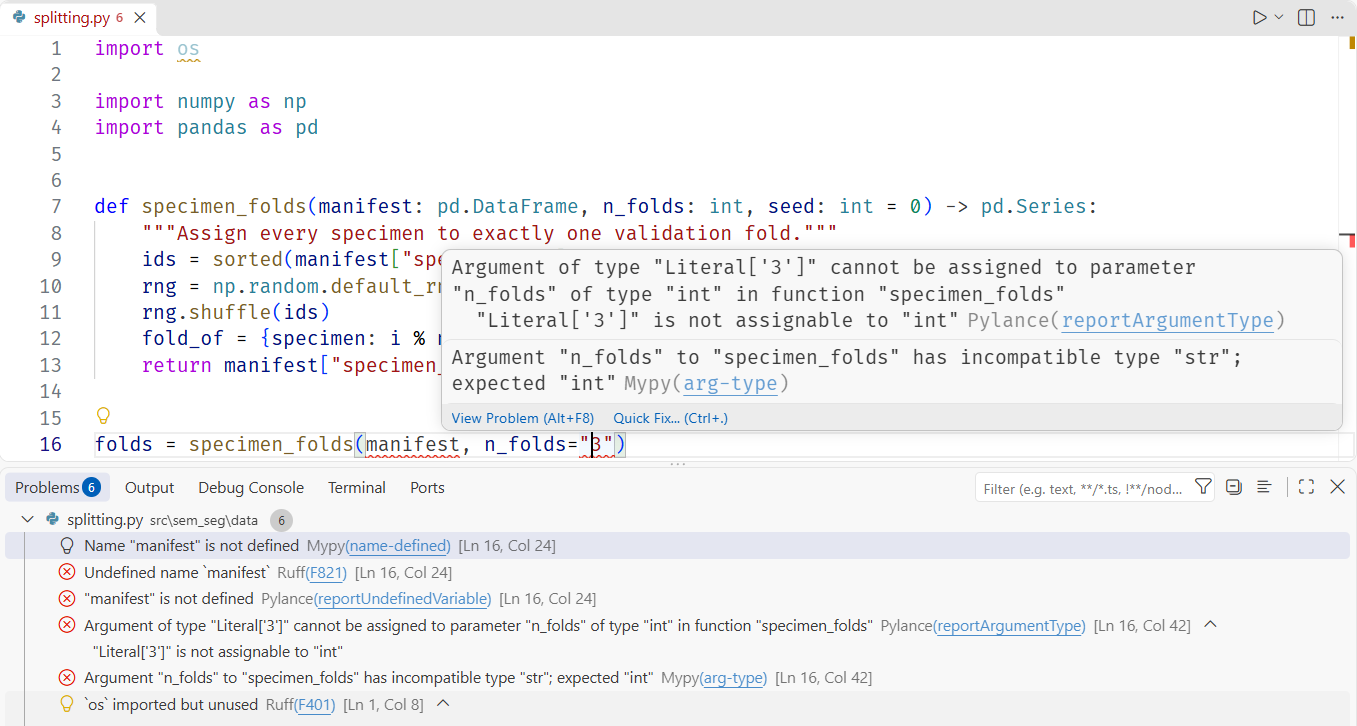
\includegraphics[width=\linewidth]{assets/screens/vscode-lint.png}};
        \begin{scope}[x={(img.south east)},y={(img.north west)}]
          \node[number mark] at (0.179,0.963) {1};
          \node[number mark] at (0.849,0.698) {2};
          \node[number mark] at (0.111,0.328) {3};
        \end{scope}
      \end{tikzpicture}
    \end{column}
    \begin{column}{0.27\textwidth}
      % each item numbered by its marker on the screenshot
      \footnotesize
      \begin{itemize}\setlength\itemsep{2mm}
        \item[\numbermark{1}] Ruff: unused import (\fn{F401}), undefined name (\fn{F821})
        \item[\numbermark{2}] Pylance and mypy: a string passed as \fn{n\_folds}
        \item[\numbermark{3}] Problems panel: every finding, with its tool and rule
      \end{itemize}
    \end{column}
  \end{columns}
  \note{\textbf{8:00--8:40}\par
    A real screenshot: VS Code 1.142 with the Ruff, Pylance and Mypy extensions on a
      deliberately broken version of our split function.\par
    Squiggles mark the unused import, the undefined name and the wrong argument type; hovering
      shows the message and which tool raised it.\par
    The Problems panel lists all six findings, each with its tool and rule, so you can look up
      or switch off a rule.\par
    The agent sees the same findings when it runs the tools from the terminal.}
\end{frame}

% ------------------------------------------------------------ set up once
\begin{frame}[fragile,source={Astral (2026), Ruff: editor setup · Microsoft (2026), Mypy Type Checker; Pylance README}]{Set them up once}
  % left: the tools on the command line; right: the same tools in VS Code. The right column is
  % wide enough for the longest line of settings.json (55 characters at 7 pt) on one line; the
  % left one then holds 42 characters of code and a table whose widest label is "Format".
  \begin{columns}[T,onlytextwidth]
    \begin{column}{0.425\textwidth}
\begin{codefile}[style=sh,basicstyle=\ttfamily\fontsize{7}{8.4}\selectfont]{pyproject.toml}
[tool.ruff]  # rules: Ruff's defaults
line-length = 100

[tool.mypy]
python_version = "3.12"
\end{codefile}
      \scriptsize\renewcommand\arraystretch{1.4}\setlength\tabcolsep{3pt}
      \begin{tabularx}{\linewidth}{@{}>{\bfseries}l>{\ttfamily}X@{}}
        \toprule
        Install        & conda install -c conda-forge ruff mypy\\
        \midrule
        Lint           & ruff check --fix\\
        Format         & ruff format\\
        Types          & mypy src\\
        \bottomrule
      \end{tabularx}
    \end{column}
    \begin{column}{0.545\textwidth}
\begin{codefile}[basicstyle=\ttfamily\fontsize{7}{8.4}\selectfont]{.vscode/settings.json}
{
  "[python]": {
    "editor.defaultFormatter": "charliermarsh.ruff",
    "editor.formatOnSave": true,
    "editor.codeActionsOnSave": {
      "source.fixAll": "explicit",
      "source.organizeImports": "explicit"}},
  "python.analysis.typeCheckingMode": "standard",
  "mypy-type-checker.importStrategy": "fromEnvironment"
}
\end{codefile}
      \footnotesize
      \begin{itemize}\setlength\itemsep{1mm}
        \item VS Code extensions: Python (brings Pylance), Ruff, Mypy Type Checker
        \item pick the environment: \emph{Python: Select Interpreter}
        \item the same commands go into \fn{AGENTS.md}
      \end{itemize}
    \end{column}
  \end{columns}
  \note{\textbf{8:40--9:40}\par
    Set up once per repository, then it runs by itself.\par
    The tool settings live in pyproject.toml, which works for conda projects too.\par
    One conda command installs both; by hand, three commands lint, format and type-check.\par
    In VS Code, install the Python extension, which brings Pylance, plus the Ruff and Mypy Type
      Checker extensions, and select the project's environment.\par
    The workspace settings make Ruff format and fix on every save, switch Pylance's type
      checking on, and make the Mypy extension use the mypy installed in the environment rather
      than the older copy it bundles.\par
    The same commands go into AGENTS.md, so the agent runs them too.}
\end{frame}

\section[Repository]{Preparing the repository}
\sectionframe{03}{Preparing the repository}
  {What can the repository tell the agent, so that we do not have to?}
  {\faFolderOpen}

% ------------------------------------------------------ the layout and its files
% Left: a standard layout, adapted from Cookiecutter Data Science, with one AGENTS.md. Right: the
% same repository later, its AGENTS.md split into three files. One picture, so that the arrow can
% run from one tree to the other: the rows are the theme's folder-tree rows, the pages are drawn
% here. Both trees start at the same height with a row pitch of 3.5 mm; the arrow leaves the
% AGENTS.md row on the left (row 9, y = -12.6 - 8 * 3.5) for rows 5 to 7 on the right.
\begin{frame}[source={DrivenData (2026), Cookiecutter Data Science}]{Setting up the repository}
  \begin{tikzpicture}[x=1mm,y=1mm,
      head/.style={anchor=north west,inner sep=0pt,font=\small\bfseries,text=udsdark},
      page/.style={draw=udsgreylight,fill=white,line width=0.5pt,rounded corners=1.2mm},
      split/.style={udsblue,line width=0.9pt},
      splitarrow/.style={split,-{Stealth[length=2mm,width=1.6mm]}}]
    \useasboundingbox (0,0) rectangle (144,-55);
    % ---- left: the layout, and a link to the template it follows
    \node[head] at (0,0) {A standard layout};
    \node[anchor=north west,inner sep=0pt,font=\footnotesize] at (0,-4.6)
      {\href{https://cookiecutter-data-science.drivendata.org/\#directory-structure}%
        {\faGlobe\enspace\underline{\fn{cookiecutter-data-science}}}};
    \draw[page] (0,-9.4) rectangle (60,-54.4);
    \begin{scope}[shift={(2.4,-12.6)}]
      \treestart{note at=30,row height=3.5}
      \tdir{0}{sem-seg/}{}
      \tdir{1}{data/raw/}{never edited}
      \tdir{1}{data/processed/}{made by the code}
      \tdir{1}{models/}{trained models}
      \tdir{1}{notebooks/}{exploring}
      \tdir{1}{reports/figures/}{figures for papers}
      \tdir{1}{src/sem\_seg/}{the code}
      \tdir{1}{tests/}{}
      \tfile{1}{\textcolor{udsblue}{\textbf{AGENTS.md}}}{\textcolor{udsblue}{for the agent}}
      \tfile{1}{environment.yml}{}
      \tfile{1}{pyproject.toml}{}
      \tfile{1}{README.md}{for people}
    \end{scope}
    % ---- right: the same repository once AGENTS.md has grown; what stays the same in grey
    \node[head] at (74,0) {As the project grows};
    \draw[page] (74,-9.4) rectangle (144,-40.3);
    \begin{scope}[shift={(76.4,-12.6)}]
      \treestart{note at=33.6,row height=3.5}
      \tdir{0}{sem-seg/}{}
      \tdirgrey{1}{data/ \dots}{as before}
      \tdirgrey{1}{models/ \dots\ reports/}{}
      \tdirgrey{1}{src/sem\_seg/, tests/}{}
      \tfile{1}{\textcolor{udsblue}{\textbf{AGENTS.md}}}{commands, rules, pointers}
      \tfile{1}{GLOSSARY.md}{the project's words}
      \tfile{1}{CODING\_STANDARDS.md}{how code is written here}
      \tfilegrey{1}{environment.yml, \dots}{}
    \end{scope}
    \node[anchor=north west,inner sep=0pt,font=\footnotesize,text=udsdark,text width=70mm,
      align=left] at (74,-43.4) {\fn{AGENTS.md} keeps what every session needs and points to
      the two new files};
    % ---- one file becomes three: from the AGENTS.md row on the left to rows 5 to 7 on the right
    \draw[split] (49.5,-40.6) -- (62,-40.6);% starts clear of the note "for the agent"
    \foreach \y in {-26.6,-30.1,-33.6} \draw[splitarrow] (62,-40.6) to[out=0,in=180] (74,\y);
  \end{tikzpicture}
  \note{\textbf{9:50--10:50}\par
    Before any file for the agent: a layout that people and agents already know.\par
    This one follows Cookiecutter Data Science, a template for data projects, with the code in
      src and its tests beside it: raw data that is never edited, processed data that the code
      makes, models, notebooks for exploring, figures for papers.\par
    An agent finds its way in it the way a new colleague does.\par
    At the root sits AGENTS.md, the one file written for the agent.\par
    As the project grows, AGENTS.md keeps what every session needs, and two files take the rest:
      GLOSSARY.md for the project's words, CODING\_STANDARDS.md for how code is written here.}
\end{frame}

% --------------------------------------------------------------- AGENTS.md
% The example file beside what such a file should hold and leave out, after the prompting guides
% of Anthropic and OpenAI (SOURCES.md)
\begin{frame}[fragile,source={Anthropic (2026), Prompting Claude Opus 5.5 · OpenAI (2026), Using GPT-6}]{\texttt{AGENTS.md}}
  \begin{columns}[T,onlytextwidth]
    \begin{column}{0.57\textwidth}
\begin{codefile}[basicstyle=\ttfamily\fontsize{7.2}{8.75}\selectfont]{AGENTS.md}
# sem-seg
## Setup and checks
- Environment: conda env `sem-seg`, activated beforehand
- Fast check (CPU, synthetic data): `pytest -q`
- Lint, types: `ruff check`, `mypy src` §\textcolor{udsred}{\sffamily\scriptsize\faArrowLeft\ after every edit}§
## Conventions
- Terms: `GLOSSARY.md` (specimen, micrograph, patch) §\smash{\textcolor{udsblue}{\faLink}}§
- Decisions: `docs/adr/` §\smash{\textcolor{udsblue}{\faLink}}§
- Lengths in micrometres; pixel size from metadata
## Boundaries
- Never write to `data/raw/`; use `data/processed/`
- No cluster jobs (`sbatch`): the queue is shared
- Ask before adding a dependency
## When you finish
- Report changed files, checks run, open assumptions
\end{codefile}
    \end{column}
    \begin{column}{0.40\textwidth}
      \begin{tikzpicture}[x=1mm,y=1mm,
          head/.style={anchor=north west,inner sep=0pt,font=\footnotesize\bfseries},
          item/.style={anchor=north west,inner sep=0pt,font=\footnotesize,text=udsdark},
          why/.style={anchor=north west,inner sep=0pt,font=\scriptsize,text=udsgrey}]
        \useasboundingbox (0,0) rectangle (57,-54);
        \node[head,text=testgreen] at (0,0) {Put in};
        \foreach \t [count=\i] in {{commands to set up, test and check},
            pointers to what the code cannot show,what needs your approval,
            {when it is done, and what to report},the reason behind a rule}
          \node[item] at (0,-0.7-\i*4.3) {\textcolor{testgreen}{\faCheck}\enspace\t};
        \node[head,text=udsred] at (0,-27.8) {Leave out};
        \foreach \t/\w [count=\i] in {{rules that clash or are out of date}/{the agent may stop and wait},
            {vague wishes: ``write clean code''}/{name the exact mistake instead},
            {``think carefully'', ``be thorough''}/{current models already do}} {
          \node[item] at (0,-25-\i*7.6) {\textcolor{udsred}{\faTimes}\enspace\t};
          \node[why] at (4.3,-28.8-\i*7.6) {\w};
        }
      \end{tikzpicture}
    \end{column}
  \end{columns}
  \note{\textbf{10:50--12:10}\par
    AGENTS.md is the one file that tools supporting it load at the start of every session.\par
    It holds what the agent cannot find out alone: the commands to set up, test and check; what
      the code cannot show, or which file shows it; what needs our approval; when the work is done
      and what to report.\par
    Fifteen lines, each preventing a specific mistake, and one says why: the cluster queue is
      shared.\par
    The checks of section 2 are here, so the agent runs them after every edit; the boundaries are
      requests, not locks.\par
    Today's models follow such files closely: OpenAI notes that its latest model is more
      sensitive to files such as AGENTS.md, and that unclear or conflicting guidance can make it
      stop early.\par
    So leave out rules that clash or are out of date; vague wishes such as write clean code,
      where naming the exact mistake works better; and lines such as think carefully, which
      Anthropic advises removing from system prompts, since the model decides how much to
      think.\par
    Keep it short, and review it like code.}
\end{frame}

% ---------------------------------------------------- glossary, standards
% \tagchip{text}: a tag naming what a file holds
\newcommand\tagchip[1]{\tikz[baseline=(t.base)]\node[draw=udsblue,fill=bluetint,line width=0.4pt,
  rounded corners=0.6mm,inner xsep=1mm,inner ysep=0.5mm,font=\scriptsize,text=udsdark] (t) {#1};}
\begin{frame}[fragile,source={Pocock (2026), mattpocock/skills v1.3.1: domain-modeling, code-review, retro}]{\texttt{GLOSSARY.md} and \texttt{CODING\_STANDARDS.md}}
  \begin{columns}[T,onlytextwidth]
    \begin{column}{0.485\textwidth}
      {\scriptsize\color{udsgrey}holds\enspace}\tagchip{term and meaning}\enspace
        \tagchip{words to avoid}\enspace\tagchip{code name}\par\vskip1.6mm
\begin{codefile}[basicstyle=\ttfamily\fontsize{7}{8.5}\selectfont]{GLOSSARY.md\enspace\textcolor{udsgreymid}{\sffamily\scriptsize read when pointed to}}
# Glossary
Specimen: one physical sample (`specimen_id`).
  Avoid: §\textcolor{udsred}{\bfseries sample}§, coupon. §\textcolor{udsred}{\sffamily\scriptsize\faArrowLeft\ the word in our request}§
Area: one imaged region of a specimen.
Micrograph: one SEM image of an area
  (`micrograph_id`). Avoid: image, frame.
Patch: a crop of a micrograph used in
  training (`patch_id`). Avoid: tile.
Fold: specimens held out together; every
  specimen belongs to exactly one fold.
\end{codefile}
    \end{column}
    \begin{column}{0.485\textwidth}
      {\scriptsize\color{udsgrey}holds\enspace}\tagchip{seeds}\enspace\tagchip{input checks}\enspace
        \tagchip{tests}\enspace\tagchip{paths}\par\vskip1.6mm
\begin{codefile}[basicstyle=\ttfamily\fontsize{7}{8.5}\selectfont]{CODING\_STANDARDS.md\enspace\textcolor{udsgreymid}{\sffamily\scriptsize read in review}}
# Coding standards
- Every random step takes a `seed`; the
  same seed gives the same result.
- Public functions check their inputs and
  raise `ValueError` naming the problem.
- Tests call public functions on small,
  hand-written fixtures, never real data.
- Expected values come from the fixture,
  never recomputed the way the code does.
- Paths come from `config.py`, never
  written into a function.
\end{codefile}
    \end{column}
  \end{columns}
  \note{\textbf{12:10--13:30}\par
    Two files the agent reads only when something points to them.\par
    A glossary holds the project's terms: what each one means, the words to avoid and the name the
      code uses for it; our request said sample, and here sample is a word to avoid.\par
    The clarifying step of section 7 writes terms into it as soon as they are agreed.\par
    Coding standards hold the rules a reviewer checks: seeds, input checks, how tests are built,
      where paths come from; a fixture is the small, hand-made input a test runs on.\par
    In the workflow of section 7 the review step reads it, not the implementing agent, which
      already carries the most context.\par
    Rules that a linter can check belong in Ruff's settings instead, so that every run checks
      them.}
\end{frame}

\section[Decisions]{Architecture Decision Records (ADRs)}
\sectionframe{04}{Architecture Decision Records (ADRs)}
  {Why does the project work this way, and what if we change our minds?}
  {\faBalanceScale}

% ------------------------------------------------------------ what / when
\begin{frame}[source={Nygard (2011), Documenting architecture decisions · Pocock (2026), mattpocock/skills v1.3.1, domain-modeling}]{What an ADR is, and when to write one}
  \begin{tikzpicture}[x=1mm,y=1mm,
      crit/.style={inner sep=0pt,font=\footnotesize,text=udsdark,align=center},
      item/.style={anchor=base west,inner sep=0pt,font=\footnotesize,text=udsdark}]
    % the record itself: Nygard's format
    \node[anchor=north west,inner sep=0pt,font=\footnotesize,text=udsdark] at (0,0)
      {\textbf{One decision per record:}\enspace title · context · decision · status ·
       consequences; numbered; superseded records stay};
    % write one only where all three hold; each label sits in its circle's own part
    \coordinate (A) at (17,-22); \coordinate (B) at (35,-22); \coordinate (C) at (26,-37.6);
    \foreach \p in {A,B,C}
      \filldraw[draw=udsblue,line width=0.7pt,fill=udsblue,fill opacity=0.09] (\p) circle (15);
    \node[crit] at (11.5,-19.5) {hard to\\reverse};
    \node[crit] at (40.5,-19.5) {surprising\\without\\context};
    \node[crit] at (26,-44) {a real\\trade-off};
    \node[inner sep=0.4mm,font=\small\bfseries,text=udsred] (adr) at (26,-27.2) {ADR};
    % where all three usually hold in research code, level with the circles' top
    \node[anchor=north west,inner sep=0pt,font=\footnotesize\bfseries,text=udsdark] at (70,-7)
      {typical in research code};
    \foreach \t [count=\i] in {the split unit and the evaluation protocol,merged or remapped classes,
        {units, scales, normalisation},the metric that decides what is ``better''}
      \node[item] at (72,-9.2-\i*5.4) {\textcolor{udsred}{\faAngleRight}\enspace\t};
    \draw[udsred,line width=0.6pt] (adr.east) to[out=0,in=180] (69.4,-21.7);
    \node[anchor=base west,inner sep=0pt,font=\scriptsize,text=udsgrey] at (72,-41)
      {no ADR: plot styling, renames};
  \end{tikzpicture}
  \note{\textbf{13:40--14:40}\par
    An architecture decision record keeps one decision with its reasons.\par
    Nygard's format: title, context, decision, status and consequences, including the bad
      ones.\par
    Records are numbered in sequence, numbers are never reused, and a superseded record stays in
      the repository.\par
    A useful test, from the skills of section 7: write one only when the decision is hard to
      reverse, would surprise a newcomer, and came from a real trade-off.\par
    In research code that is usually about what a number means: the split unit, class
      definitions, units and normalisation, the metric.\par
    Plot styling and renames do not need one.}
\end{frame}

% ------------------------------------------------------------- ADR example
\begin{frame}[fragile]{ADR-0003: specimen-level splits}
  \begin{columns}[T,onlytextwidth]
    \begin{column}{0.58\textwidth}
\begin{codefile}[basicstyle=\ttfamily\fontsize{7}{8.4}\selectfont]{docs/adr/0003-specimen-level-splits.md}
# ADR-0003: Specimen-level splits
Status: accepted. Supersedes ADR-0001 (random patch split).
## Context
Micrographs of one specimen share preparation and etching;
several show the same area. A random patch split puts this
material in training and validation.
## Decision
Specimens are assigned to validation folds; each patch
inherits its specimen's fold. Folds are saved with seed
and manifest hash and checked for overlap.
## Considered options
Random patch split; split by micrograph. Both leak.
## Consequences
Few independent units: report every fold and its spread.
One specimen per state: a held-out specimen is a new state.
\end{codefile}
    \end{column}
    \begin{column}{0.39\textwidth}
      \begin{tikzpicture}[x=1mm,y=1mm]
        \node[artifact,anchor=north west,text width=50mm,align=left,font=\scriptsize] (a1) at (0,0)
          {\texttt{0001-random-patch-split.md}\\[0.4mm]
           \textcolor{udsred}{Status: superseded by ADR-0003}};
        \node[artifact,anchor=north west,text width=50mm,align=left,font=\scriptsize,draw=udsblue,fill=bluetint] (a3) at (0,-16)
          {\texttt{0003-specimen-level-splits.md}\\[0.4mm]
           \textcolor{udsblue}{Status: accepted}};
        \draw[flow] (a3.north) -- node[lbl,right]{supersedes} (a1.south);
        \node[anchor=north west,text width=54mm,font=\scriptsize,inner sep=0pt] at (0,-27.5)
          {ADR-0001 stays: it shows what was tried and why it changed.};
      \end{tikzpicture}\par\vskip3mm
      \begin{panel}[fontupper=\footnotesize,colback=bluetint,borderline west={1.2mm}{0pt}{udsblue},left=3.5mm]
        An agent chasing a better score finds ADR-0003 through \fn{AGENTS.md} before it brings back a
        random split.
      \end{panel}
    \end{column}
  \end{columns}
  \note{\textbf{14:40--15:40}\par
    The record for our running example.\par
    The context explains why a random patch split misleads here; the decision is short and
      testable; the considered options show that splitting by micrograph was rejected for the
      same reason.\par
    The consequences are honest: few specimens mean few independent units, and with one specimen
      per material state every held-out specimen is also a new state.\par
    ADR-0001 is not deleted; its status points to its successor.\par
    An agent tuning for a better score finds this record before it undoes the decision.}
\end{frame}

% ------------------------------------------------------------- file roles
\begin{frame}[source={OpenAI (2026), Custom instructions with AGENTS.md · Pocock (2026), mattpocock/skills v1.3.1: code-review; v1.3 changelog}]{When the agent reads each file}
  % the files of sections 3 and 4, the README and the task specification of section 1, placed on
  % an agent session at the moment each one is read
  \begin{tikzpicture}[x=1mm,y=1mm,
      chip/.style={draw=udsgreylight,fill=white,rounded corners=0.6mm,inner xsep=1mm,inner ysep=0.8mm,
        anchor=north west,font=\ttfamily\fontsize{7.4}{8.4}\selectfont,text=udsdark,line width=0.5pt,
        path picture={\draw[udsblue,line width=0.9pt] (path picture bounding box.north west)
          -- (path picture bounding box.north east);}},
      always/.style={chip,draw=udsblue,line width=0.9pt},
      ondemand/.style={chip,dashed,draw=udsdark,path picture={}},
      reviewstep/.style={chip,draw=udsblue,fill=bluetint,path picture={},font=\footnotesize},
      say/.style={anchor=north west,inner sep=0pt,font=\scriptsize,text=udsdark,align=left,text width=30mm,
        execute at begin node={\hyphenpenalty=10000\raggedright}},
      drop/.style={udsgreymid,line width=0.5pt},
      dot/.style={circle,fill=udsdark,inner sep=0pt,minimum size=1.8mm}]
    % AGENTS.md points to the glossary and the ADRs
    \node[always] (ag) at (0,-4.6) {AGENTS.md};
    \node[ondemand] (gl) at (44,-4.6) {GLOSSARY.md};
    \node[ondemand] (ad) at (78,-4.6) {docs/adr/};
    \draw[drop,dashed] (ag.north) |- (ad.north |- 0,-1.6);
    \foreach \n in {gl,ad} \draw[drop,dashed,-{Stealth[length=1.6mm,width=1.2mm]}] (\n.north |- 0,-1.6) -- (\n.north);
    \node[anchor=south,inner sep=0.5mm,font=\scriptsize,text=udsgrey,fill=white] at (27,-1.6) {points to};
    \node[say] at ([yshift=-1.2mm]ag.south west) {\textcolor{udsblue}{\bfseries every session}\\ commands, boundaries, pointers};
    \node[say] at ([yshift=-1.2mm]gl.south west) {\textbf{when pointed to}\\ domain terms};
    \node[say] at ([yshift=-1.2mm]ad.south west) {\textbf{when pointed to}\\ one decision and its reasons};
    % read in review
    \node[chip] (cs) at (112,-4.6) {CODING\_STANDARDS.md};
    \node[say] at ([yshift=-1.2mm]cs.south west) {\textbf{in review}\\ how code is written here};
    % the session, left to right, and where each file enters it
    \draw[flow,line width=0.9pt] (0,-27) -- (143.4,-27);% the tip stays inside the text width
    \node[anchor=south west,inner sep=0.6mm,font=\scriptsize,text=udsgrey] at (12,-27) {an agent session};
    \foreach \n in {ag,gl,ad,cs} {\node[dot] at (\n.south |- 0,-27) {}; \draw[drop] (\n.south |- 0,-21.6) -- (\n.south |- 0,-27);}
    % the task's own specification comes with it; the review checks the code against the standards
    \node[chip,font=\footnotesize] (sp) at (0,-32) {task specification};
    \node[say] at ([yshift=-1.2mm]sp.south west) {\textbf{with the task}\\ objective, acceptance criteria};
    \draw[drop] (ag.south |- 0,-27) -- (ag.south |- sp.north);
    \node[reviewstep] (cr) at (112,-32) {\faSearch\enspace review};
    \node[say] at ([yshift=-1.2mm]cr.south west) {a person or an agent checks the code against it};
    \draw[drop] (cs.south |- 0,-27) -- (cs.south |- cr.north);
    % read like any other file
    \node[chip,draw=udsgreylight,text=udsgrey,path picture={}] (rd) at (44,-34) {README.md};
    \node[say,text=udsgrey,text width=40mm,anchor=west] at ([xshift=2mm]rd.east) {for people; read like any other file};
  \end{tikzpicture}
  \note{\textbf{15:40--16:30}\par
    Each file on one agent session, at the moment it is read.\par
    AGENTS.md at the start of every session; the glossary and the ADRs when AGENTS.md points to
      them.\par
    The task specification of section 1 comes with the task; the coding standards are read when
      the change is reviewed, by a person or an agent.\par
    The README is for people; the agent reads it like any other file.\par
    Keep each fact in one place and link to it: copies go stale.}
\end{frame}

% ------------------------------------ the specification of section 1, remembered
% Slide 5's five cards again, greyed: the theme's colours are redefined for one group only, so the
% same macros draw them. A stamp repeats slide 5's warning; the strip says where the parts that
% repeat are now, which the next slide shows card by card.
\begin{frame}{Remember the bounded task specification?}
  \begin{tikzpicture}[x=1mm,y=1mm]
    \useasboundingbox (0,0) rectangle (144,-54);
    \begingroup
      \colorlet{udsblue}{udsgreymid}\colorlet{udsdark}{udsgreymid}
      \foreach \k/\l in {0/Objective,1/Context,2/Constraints,3/Acceptance,4/Verification}
        {\speccard{\k}{0}{-41.4}{\l}{udsgreypale!60}}
      \foreach \k/\t in {
          0/{add \fn{specimen\_folds()} to \fn{src/sem\_seg/\allowbreak data/\allowbreak splitting.py}; use it
            in the training CLI as \fn{--split specimen}},
          1/{``sample'' means specimen: one physical sample, column \fn{specimen\_id} of the manifest},
          2/{leave \fn{data/raw/} and the manifests unchanged; no new dependencies; no GPU jobs},
          3/{each specimen in exactly one fold; each patch inherits its specimen's fold; same seed, same
            folds; \fn{ValueError} if \fn{specimen\_id} is missing or there are fewer specimens than folds},
          4/{\fn{pytest tests/data -q} passes; report changed files, test output and assumptions}}
        \node[spec body] at (b\k) {\t};
    \endgroup
    % slide 5's warning, stamped across the cards
    \node[rotate=7,draw=udsred,double=white,double distance=0.7pt,line width=0.8pt,
      rounded corners=1mm,fill=white,fill opacity=0.88,text opacity=1,text=udsred,
      font=\large\bfseries,inner xsep=3mm,inner ysep=2.2mm] at (72,-21)
      {\faExclamationTriangle\enspace too much to write for every task};
    % where those parts are now
    \fill[bluetint] (0,-48.4) rectangle (144,-54);
    \fill[udsblue] (0,-48.4) rectangle (1.2,-54);
    \node[anchor=west,inner sep=0pt,font=\footnotesize,text=udsdark] at (3.6,-51.2)
      {\textcolor{udsblue}{\faCheck}\enspace what repeats is now in files: \fn{AGENTS.md},
       \fn{GLOSSARY.md}, ADRs, \fn{CODING\_STANDARDS.md}};
  \end{tikzpicture}
  \note{\textbf{16:30--17:00}\par
    Remember the bounded specification from the start of the talk.\par
    Every part of it was written by hand, for every task: what a specimen is, which data must not
      change, how to run the tests, what to report.\par
    That is the part that repeats, and it now lives in the files of sections 3 and 4.}
\end{frame}

% ------------------------------------------------ the request, revisited
\begin{frame}{The same request, in a prepared repository}
  \begin{tikzpicture}[x=1mm,y=1mm]
    % the cards fill the text width exactly; strokes on their edges must not widen the picture
    \useasboundingbox (0,0) rectangle (144,-54);
    \specterminal{0}{the request}
    \node[spec request] at (term) {> Add validation folds by specimen to the training CLI, as decided in ADR-0003.};
    \node[anchor=west,inner sep=0pt,font=\scriptsize\bfseries,text=udsdark] at (0,-15.8)
      {where the rest comes from};
    % the same five cards as on slides 4 and 5: the objective is the request itself, every other
    % part now comes from files
    \speccard{0}{-19}{-44.4}{Objective}{darktint}
    \foreach \k/\l in {1/Context,2/Constraints,3/Acceptance,4/Verification}
      {\specfilecard{\k}{-19}{-44.4}{\l}{darktint}}
    \node[spec chip,draw=termbg,fill=termbg,text=termfg,path picture={}] at (b0) {\faTerminal\ the request};
    % context
    \node[spec chip] (c1) at (b1) {GLOSSARY.md};
    \node[spec note] (c1s) at ([yshift=-0.8mm]c1.south west) {specimen, fold};
    \node[spec chip] (c2) at ([yshift=-2.2mm]c1s.south west) {ADR-0003};
    \node[spec note] at ([yshift=-0.8mm]c2.south west) {why; how folds are saved};
    % constraints
    \node[spec chip] (k1) at (b2) {AGENTS.md};
    \node[spec note] at ([yshift=-0.8mm]k1.south west) {boundaries};
    % acceptance
    \node[spec chip] (a1) at (b3) {ADR-0003};
    \node[spec note] (a1s) at ([yshift=-0.8mm]a1.south west) {one fold per specimen};
    \node[spec chip] (a2) at ([yshift=-2.2mm]a1s.south west) {CODING\_STANDARDS.md};
    \node[spec note] at ([yshift=-0.8mm]a2.south west) {seed, input checks};
    % verification
    \node[spec chip] (v1) at (b4) {AGENTS.md};
    \node[spec note] at ([yshift=-0.8mm]v1.south west) {fast check, report};
    % what the files leave open, the agent has to ask: the clarifying step of section 7
    \node[anchor=west,inner sep=0pt,font=\scriptsize,text=udsred] at (0,-49.4)
      {\faQuestionCircle\enspace still open: what no file says, e.g.\ the default number of folds};
  \end{tikzpicture}
  \note{\textbf{17:00--18:00}\par
    Now the same request, in the repository we prepared.\par
    With these files in place, one sentence in the project's language is enough.\par
    Four of the five parts now come from files; only the objective is in the request.\par
    The glossary says what a specimen and a fold are.\par
    ADR-0003 says why folds go by specimen and how they are saved.\par
    AGENTS.md carries the boundaries, the test command and what to report.\par
    CODING\_STANDARDS.md makes seeds and input checks part of every review.\par
    What the files leave open, here the default number of folds, is what the clarification step
      of section 7 asks.\par
    This works only while AGENTS.md points to the files and they are kept current.}
\end{frame}

\section[Version control]{Version control with git}
\sectionframe{05}{Version control with git}
  {How do we keep every version, and see exactly what an agent changed?}
  {\faCodeBranch}

% ------------------------------------------------------------- what it is
\begin{frame}[source={Chacon \& Straub (2014), Pro Git, 2nd ed., git-scm.com/book}]{Version control: one folder, every version}
  \begin{columns}[T,onlytextwidth]
    \begin{column}{0.34\textwidth}
      \begin{ablock}[equal height group=vc,fontupper=\footnotesize]{Without}
        {\ttfamily\footnotesize splitting.py\\ splitting\_old.py\\ splitting\_v2\_final.py\\
         splitting\_v2\_final\_FIXED.py\\ results\_new2/\par}\vskip2mm
        Which version produced figure 3?
      \end{ablock}
    \end{column}
    \begin{column}{0.62\textwidth}
      \begin{dblock}[equal height group=vc,fontupper=\footnotesize]{With git}
        \centering
        \begin{tikzpicture}[x=1mm,y=1mm,
            commit/.style={circle,draw=udsblue,fill=white,line width=0.9pt,minimum size=3mm,inner sep=0pt},
            bcommit/.style={commit,draw=udsred},
            msg/.style={font=\scriptsize,text=udsdark,inner sep=0.6mm}]
          \draw[udsblue,line width=1pt] (0,0) -- (51,0);
          \draw[udsred,line width=1pt] (14,0) to[out=0,in=180] (23,9) -- (42,9) to[out=0,in=180] (51,0);
          \foreach \n/\x/\t in {a/0/random split,b/14/checks,m/51/merge} {
            \node[commit] (\n) at (\x,0) {};
            \node[msg,anchor=north] at (\n.south) {\t};
          }
          \foreach \n/\x/\t in {e/25/specimen folds,f/40/tests} {
            \node[bcommit] (\n) at (\x,9) {};
            \node[msg,anchor=south] at (\n.north) {\t};
          }
          \node[font=\scriptsize\bfseries,text=udsblue,anchor=east] at (-2.5,0) {main};
        \end{tikzpicture}\par\vskip1.5mm
        \raggedright\renewcommand\arraystretch{1.15}\setlength\tabcolsep{3pt}
        \begin{tabular}{@{}>{\bfseries}l l@{}}
          commit & a snapshot with a message, an author and a date\\
          diff   & what changed between two snapshots\\
          \textcolor{udsred}{branch} & a separate line of work, merged when ready\\
          remote & a copy on a server (GitHub): backup, sharing, review\\
        \end{tabular}
      \end{dblock}
    \end{column}
  \end{columns}
  \note{\textbf{18:10--19:20}\par
    Many of us keep versions as copies: splitting old, v2, final, fixed.\par
    After a few months nobody knows which copy produced a figure.\par
    Version control replaces the copies with one folder and its history.\par
    Git stores a snapshot of the project each time you commit, with a message, an author and a
      date; a diff shows what changed between two snapshots.\par
    A branch is a separate line of work, for an experiment or for an agent's task, merged back
      when it is ready.\par
    A remote such as GitHub holds a copy of the history on a server: a backup, a way to share,
      and the place where changes are reviewed.\par
    There a branch comes back as a pull request: a request to merge it, with its diff open for
      review before it reaches main.}
\end{frame}

% ------------------------------------------------------- learning curve
\begin{frame}[fragile,source={Chacon \& Straub (2014), Pro Git, 2nd ed., git-scm.com/book · Microsoft (2026), VS Code docs: Source control}]{Getting started takes five commands}
  \edef\colgap{\the\dimexpr0.04\textwidth\relax}
  \begin{columns}[T,onlytextwidth]
    \begin{column}{0.55\textwidth}
\begin{terminal}[basicstyle=\ttfamily\fontsize{7.2}{9.2}\selectfont]{terminal}
$ git init              # once: start the history
$ git status            # what has changed?
$ git add src/ tests/   # choose what goes in
$ git commit -m "Split by specimen"
$ git push              # copy it to GitHub
\end{terminal}
      \vskip1mm
\begin{codefile}[style=sh,basicstyle=\ttfamily\fontsize{7.2}{9.2}\selectfont]{.gitignore}
data/          # raw and derived data stay out
.venv/         # environments are rebuilt, not stored
*.ckpt         # model checkpoints
.env           # secrets
.claude/worktrees/  # agent worktrees
\end{codefile}
    \end{column}
    \begin{column}{0.41\textwidth}
      \begin{tikzpicture}
        \node[anchor=south west,inner sep=0pt,draw=udsgreylight,line width=0.4pt] (img) at (0,0)
          {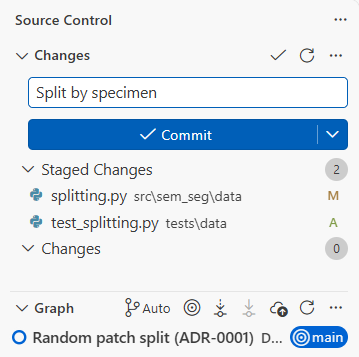
\includegraphics[height=36mm]{assets/screens/vscode-scm.png}};
        % each control, labelled with the command it replaces; push is the cloud button of the
        % graph's title row, so its line starts under that button and passes below the row
        \begin{scope}[x={(img.south east)},y={(img.north west)},
            cmd/.style={right,inner sep=0.6mm,font=\ttfamily\scriptsize,text=udsdark}]
          \foreach \y/\t in {0.683/commit,0.521/add,0.412/status}
            \draw[udsgreymid,line width=0.5pt] (1,\y) -- ++(2.5mm,0) node[cmd] {git \t};
          \draw[udsgreymid,line width=0.5pt] (0.79,0.112) |- (1,0.1) -- ++(2.5mm,0)
            node[cmd] {git push};
        \end{scope}
      \end{tikzpicture}\par\vskip1mm
      {\scriptsize VS Code's Source Control panel does the same with clicks.\par}\vskip2mm
      % the arrow spans the gap between the columns (0.04 of the text width), so it starts at the
      % edge of .gitignore; drawn by the box itself, it also lands right in the notes thumbnails
      \begin{panel}[colback=redtint,borderline west={1.2mm}{0pt}{udsred},left=3.5mm,fontupper=\footnotesize,
          overlay={\draw[flow] ([xshift=-\colgap]frame.west) -- (frame.west);}]
        data, environments and secrets do not belong in the history
      \end{panel}
    \end{column}
  \end{columns}
  \note{\textbf{19:20--20:20}\par
    The learning curve is shorter than its reputation.\par
    Five commands cover daily use: start the history once, check what changed, choose what goes
      into the next snapshot, commit it with a message, and push it to GitHub, the remote of the
      last slide.\par
    VS Code's Source Control panel does the same with buttons: here two files are staged, the
      message is typed, one click on Commit, and the cloud button pushes; the graph below is the
      history.\par
    The first push needs a repository on GitHub to push to; that cloud button, Publish Branch,
      creates one and pushes.\par
    A .gitignore file keeps out what does not belong in the history: data, environments, which
      are rebuilt from their description, model checkpoints, secrets, and the worktrees that Claude
      Code creates.\par
    Branches and merges can come later.}
\end{frame}

% ------------------------------------------------------- git and agents
\begin{frame}[source={OpenAI (2026), Agent approvals and security; Non-interactive mode · Anthropic (2026), Claude Code checkpointing}]{Why an agent needs version control}
  \begin{columns}[T,onlytextwidth]
    \begin{column}{0.66\textwidth}
      \begin{tikzpicture}
        \node[anchor=south west,inner sep=0pt,draw=udsgreylight,line width=0.4pt] at (0,0)
          {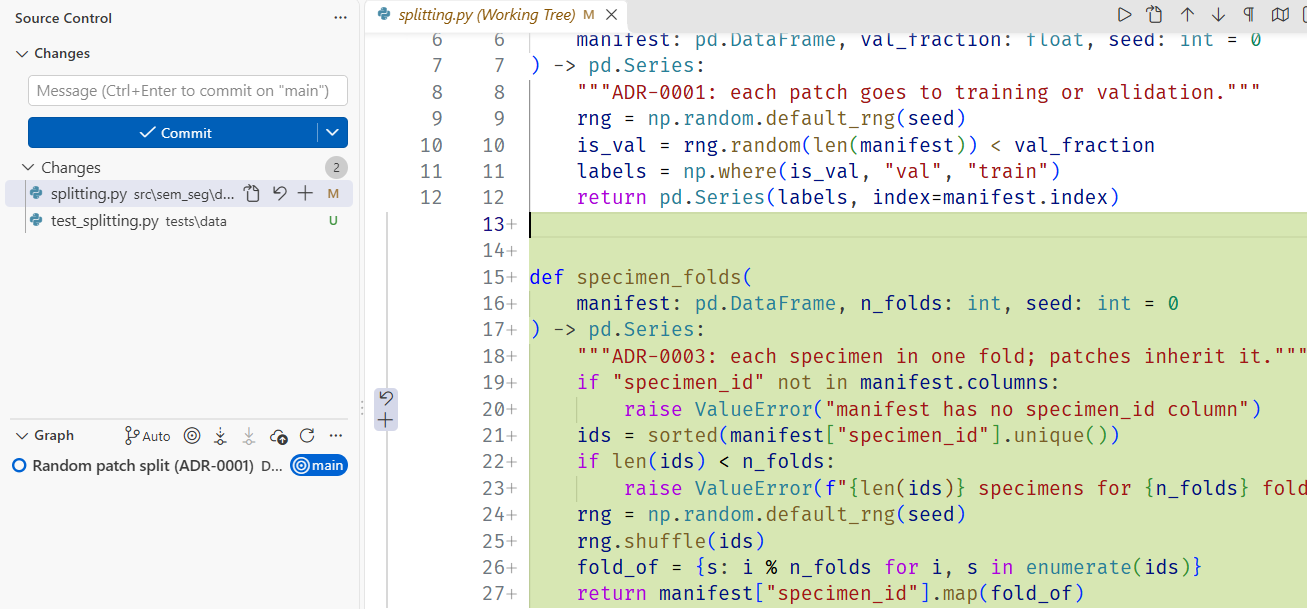
\includegraphics[width=\linewidth]{assets/screens/vscode-git.png}};
      \end{tikzpicture}\par\vskip1mm
      {\scriptsize An agent's change in VS Code's Source Control view: two files, every new line in green.\par}
    \end{column}
    \begin{column}{0.31\textwidth}
      \begin{tikzpicture}[x=1mm,y=1mm,
          commit/.style={circle,draw=udsblue,fill=white,line width=0.9pt,minimum size=3.4mm,inner sep=0pt},
          gitstep/.style={anchor=base west,inner sep=0pt,font=\footnotesize,text=udsdark,align=flush left,
            text width=38.6mm}]
        \useasboundingbox (0,0) rectangle (44.6,-52);
        % a checkpoint, the agent's uncommitted edits, then keep or discard them;
        % each label's first baseline sits 1 mm below its circle's centre
        \draw[udsblue,line width=0.9pt] (1.7,-1.9) -- (1.7,-14.4);
        \node[commit] at (1.7,-1.9) {};
        \node[gitstep] at (6,-2.9) {\textbf{checkpoint}\\commit before the agent starts};
        \node[commit,draw=udsred,dashed] (e) at (1.7,-14.4) {};
        \node[gitstep] at (6,-15.4) {\textbf{the agent's edits}\\read the diff, not the summary};
        \draw[udsblue,line width=0.9pt] (e.south) to[out=-90,in=180] (6,-27);
        \node[commit] at (7.7,-27) {};
        \node[gitstep,text width=33mm] at (11.6,-28)
          {\textbf{keep}\enspace\fn{git commit}\\{\color{udsgrey}undo later: \fn{git revert}}};
        \draw[udsgreymid,line width=0.9pt,dashed] (e.south) to[out=-90,in=180] (6,-38.6);
        \node[circle,fill=udsgreymid,text=white,inner sep=0pt,minimum size=3.4mm,font=\tiny]
          at (7.7,-38.6) {\faTimes};
        \node[gitstep,text width=33mm] at (11.6,-39.6)
          {\textbf{discard}\enspace\fn{git restore}\\{\color{udsgrey}the edits are lost}};
        \node[gitstep,text width=44.6mm,font=\footnotesize\bfseries,text=udsblue] at (0,-50.4)
          {one branch or worktree per task};
      \end{tikzpicture}
    \end{column}
  \end{columns}
  \note{\textbf{20:20--21:30}\par
    With git, an agent's work becomes a diff we can read before we accept it.\par
    Commit before the agent starts, so there is a checkpoint to return to.\par
    Read the diff itself, not the agent's summary of it: here, two files, every added line in
      green.\par
    Undo is one command: restore discards uncommitted changes for good, revert undoes a commit
      and keeps the history.\par
    A branch, or a separate worktree, per task keeps an agent's work apart from ours until it is
      reviewed.\par
    The tools assume all this.\par
    Codex checks at launch whether the folder is under version control, suggests read-only mode
      when it is not, and codex exec refuses to run outside a repository unless told
      otherwise.\par
    Claude Code can rewind its own file edits, but not files changed by shell commands, and its
      documentation says to keep using git.\par
    The workflow of section 7 commits each finished piece of work, and its review compares
      against a commit.}
\end{frame}

% ------------------------------------------------------------- worktrees
\begin{frame}[fragile,source={git documentation (2026), git-worktree · Anthropic Academy (2026)}]{Worktrees: work in parallel, merge when done}
  % the drawing carries the ideas; what a worktree is and its three commands sit beside it, level
  % with its middle
  \begin{columns}[c,onlytextwidth]
    \begin{column}{0.34\textwidth}
      \footnotesize
      \begin{itemize}\setlength\itemsep{1.5mm}
        \item a worktree: another folder of the same repository, on its own branch
        \item all folders share one history, so each branch merges into \fn{main}
      \end{itemize}\vskip2.5mm
\begin{terminal}[basicstyle=\ttfamily\fontsize{7.2}{8.5}\selectfont]{terminal}
$ git worktree add ../folds \
    -b agent/folds
$ git worktree list
$ git worktree remove ../folds
\end{terminal}
    \end{column}
    \begin{column}{0.63\textwidth}
      \centering
      \begin{tikzpicture}[x=1mm,y=1mm,
          pill/.style={rounded corners=2mm,minimum height=4mm,inner xsep=2mm,inner ysep=0.4mm,
            font=\fontsize{7}{8}\selectfont\bfseries,text=white},
          dot/.style={circle,inner sep=0pt,minimum size=2.4mm},
          tie/.style={udsgreylight,dashed,line width=0.5pt},
          card/.style={draw=udsblue,fill=bluetint,line width=0.6pt,rounded corners=1mm,
            align=left,font=\scriptsize,inner xsep=1.6mm,inner ysep=1.2mm}]
        % branches first, so that dots and cards sit on top of them
        \draw[udsblue,line width=1pt] (68,3) to[out=135,in=270] (55,20) to[out=90,in=235] (68,31);
        \draw[udsblue,line width=1pt] (68,3) to[out=162,in=270] (27,20) to[out=90,in=200] (68,42);
        \draw[udsdark,line width=1.2pt,-{Stealth[length=2.4mm,width=1.8mm]}] (68,0) -- (68,46);
        % your own folder, on main
        \node[card,draw=udsred,fill=redtint,anchor=south] at (68,46.6)
          {{\color{udsred}\faFolderOpen}\ \textbf{\fn{sem-seg/}}\quad\faCodeBranch\ \fn{main}\quad\faUser\ you};
        % commits on main, on the right; the two merges in red
        \foreach \y/\t/\c in {3/commit/udsdark,14/your commit/udsdark,31/merge/udsred,42/merge/udsred} {
          \node[dot,fill=\c] at (68,\y) {};
          \draw[tie] (69.5,\y) -- (72,\y);
          \node[pill,fill=\c,anchor=west] at (72,\y) {\t};
        }
        % one worktree per branch: its folder, its branch, its agent
        \foreach \x/\n/\b in {55/1/folds,27/2/check} {
          \node[dot,fill=udsblue] at (\x,20) {};
          \draw[tie] (\x-1.5,20) -- (\x-3,20);
          \node[card,anchor=east] at (\x-3,20)
            {{\color{udsblue}\faFolderOpen}\ \textbf{\fn{../\b}}\\ \faCodeBranch\ \fn{agent/\b}\\ \faRobot\ agent \n};
        }
      \end{tikzpicture}
    \end{column}
  \end{columns}
  \note{\textbf{21:30--22:30}\par
    A worktree is a second working folder of the same repository, checked out on its own
      branch.\par
    Each card is one: a folder next to the repository, its branch, and the agent working in it;
      your own folder, sem-seg, is the main worktree on main.\par
    Both agents start from the same commit on main and work at the same time, while you keep
      committing on main in your own folder.\par
    When an agent's work is reviewed, its branch is merged into main: first one, then the
      other.\par
    All worktrees share one history, and git lets a branch be checked out in only one worktree
      at a time, so the agents get in neither each other's way nor yours.\par
    Three commands: add creates the folder and the branch, list shows them, remove deletes the
      folder once its branch is merged.}
\end{frame}

% ------------------------------------------- worktrees in the app and the terminal
\begin{frame}[source={Anthropic (2026), Claude Code docs: Desktop; Worktrees; CLI reference}]{How to use worktrees?}
  \begin{tikzpicture}[x=1mm,y=1mm,
      head/.style={anchor=north west,inner sep=0pt,font=\small\bfseries,text=udsdark},
      stage/.style={circle,fill=udsblue,text=white,inner sep=0pt,minimum size=5.6mm,font=\scriptsize},
      txt/.style={anchor=north west,inner sep=0pt,font=\footnotesize,text=udsdark,align=flush left,
        text width=61mm},
      mono/.style={anchor=west,inner sep=0pt,font=\ttfamily\fontsize{7}{8}\selectfont}]
    \useasboundingbox (0,0) rectangle (144,-55);
    \node[head] at (8,0) {Claude app};
    \node[head] at (83,0) {Terminal};
    \draw[udsgreylight,line width=0.4pt] (72,0) -- (72,-54.6);
    % the app: Worktree on under the prompt box (screenshot), with a red box on the button
    \node[anchor=north west,inner sep=0pt,draw=udsgreylight,line width=0.4pt] (app) at (8,-4.6)
      {
\includegraphics[width=61mm]{assets/screens/claude-app-worktree.png}};
    \begin{scope}[shift={(app.south west)},x={($(app.south east)-(app.south west)$)},
        y={($(app.north west)-(app.south west)$)}]
      \draw[udsred,line width=1.1pt] (0.552,0.01) rectangle (0.809,0.35);
    \end{scope}
    % the terminal: the session's own branch, as Claude Code shows it
    \fill[termbg,rounded corners=1.2mm] (83,-4.6) rectangle (144,-19.04);
    \foreach \c [count=\i] in {termdot1,termdot2,termdot3} \fill[\c] (83.4+\i*2.3,-7.2) circle (0.7);
    \node[inner sep=0pt,font=\ttfamily\fontsize{7}{8}\selectfont,text=termdim] at (113.5,-7.2)
      {claude --worktree specimen-folds};
    \draw[white!18!termbg,line width=0.4pt] (83,-9.8) -- (144,-9.8);
    \node[mono,text=termfg] at (85.6,-12.9) {! git branch --show-current};
    \node[mono,text=termfg] at (85.6,-16.4) {\phantom{! }└ worktree-specimen-folds};
    \draw[udsred,line width=1.1pt] (84.6,-10.9) rectangle (124.4,-18.4);
    \node[anchor=north west,inner sep=0pt,font=\scriptsize,text=udsgrey] at (8,-20.6)
      {\textbf{Worktree}: ``Work in an isolated copy of the repository''};
    \node[anchor=north west,inner sep=0pt,font=\scriptsize,text=udsgrey] at (83,-20.6)
      {the session runs on its own branch};
    % one session, start to end: the same four stages, with their icons, in both columns
    \foreach \x in {2.8,77.8} {
      \draw[udsgreylight,line width=1.2pt] (\x,-28.7) -- (\x,-51.5);
      \foreach \y/\icon in {-28.7/\faPlay,-36.3/\faFolderOpen,-43.9/\faClone,-51.5/\faFlagCheckered}
        \node[stage] at (\x,\y) {\icon};
    }
    \node[txt] at (8,-25.4) {\textbf{+ New} or Ctrl+N, then \textbf{Worktree}\\
      {\scriptsize\color{udsgrey}off by default, or on per saved environment}};
    \node[txt] at (83,-25.4) {\fn{claude -w specimen-folds}\\
      {\scriptsize\color{udsgrey}first time: trust the folder once}};
    \node[txt] at (8,-33.0) {\fn{.claude/worktrees/<name>/}\\
      \textcolor{udsblue}{\faCodeBranch}\ \fn{claude/<name>}};
    \node[txt] at (83,-33.0) {\fn{.claude/worktrees/specimen-folds/}\\
      \textcolor{udsblue}{\faCodeBranch}\ \fn{worktree-specimen-folds}};
    \node[txt] at (8,-40.6) {next task: the same again\\
      {\scriptsize\color{udsgrey}the sessions run side by side}};
    \node[txt] at (83,-40.6) {another terminal, another name\\
      {\scriptsize\color{udsgrey}another agent}};
    % one line each, centred on its icon
    \node[txt,anchor=mid west] at (8,-51.5) {\textbf{Create PR}, merge, \textbf{Archive}};
    \node[txt,anchor=mid west] at (83,-51.5) {exit};
  \end{tikzpicture}
  \note{\textbf{22:30--24:00}\par
    Each session can run in its own worktree, from the Claude app or from the terminal.\par
    In the app: New or Ctrl+N, then turn on Worktree under the prompt box; it is off by default,
      so without it the agent edits your own checkout.\par
    A saved environment can switch it on for every session; Settings, Claude Code, sets the
      worktree location and the branch prefix.\par
    In the terminal: the flag worktree, or w, with a name; the first time, run claude once and
      trust the folder.\par
    Either way each session gets its own folder under .claude/worktrees and its own branch, so the
      agents run side by side.\par
    App sessions end with a pull request, a merge and Archive; uncommitted changes are kept for
      about thirty days.\par
    Leaving a terminal session removes an unchanged worktree and asks about a changed one.}
\end{frame}

% ------------------------------------------- tip: fork a session, then a worktree per fork
% Top: one session's conversation, forked in two; each fork asks for a worktree (Claude Code's
% EnterWorktree tool) and works in a folder of its own. Bottom: the Claude app's sidebar with a
% session and the sessions forked from it, numbered as in its key, and the same in a terminal.
\begin{frame}[source={Anthropic (2026), Claude Code docs: Sessions; Worktrees; CLI reference}]{Tip: when a session splits into two tasks, fork it}
  \begin{tikzpicture}[x=1mm,y=1mm,
      msg/.style={circle,fill=udsdark,inner sep=0pt,minimum size=2.2mm},
      lane/.style={udsdark,line width=1pt},
      ask/.style={human,anchor=west,font=\scriptsize,inner xsep=1.4mm,inner ysep=1mm,
        rounded corners=1mm},
      wt/.style={draw=udsblue,fill=bluetint,line width=0.6pt,rounded corners=1mm,anchor=west,
        align=left,font=\scriptsize,text=udsdark,inner xsep=1.6mm,inner ysep=1.2mm},
      head/.style={anchor=north west,inner sep=0pt,font=\small\bfseries,text=udsdark},
      key/.style={anchor=west,inner sep=0pt,font=\footnotesize,text=udsdark,align=left,
        text width=35mm},
      mono/.style={anchor=west,inner sep=0pt,font=\ttfamily\fontsize{7}{8}\selectfont}]
    \useasboundingbox (0,0) rectangle (144,-55);
    % one session: its conversation so far, then the fork
    \draw[lane] (1.1,-12) -- (50,-12);
    \foreach \x in {1.1,9.7,18.3,26.9,35.5,44.1} \node[msg] at (\x,-12) {};
    \node[anchor=base west,inner sep=0pt,font=\footnotesize\bfseries,text=udsdark] at (0,-7.8)
      {one session};
    \node[anchor=north west,inner sep=0pt,font=\scriptsize,text=udsgrey] at (0,-14.8)
      {its conversation, kept by both forks};
    \node[circle,fill=udsred,text=white,inner sep=0pt,minimum size=5.6mm,font=\scriptsize] (fk)
      at (52.8,-12) {\faClone};
    \node[anchor=base,inner sep=0pt,font=\ttfamily\footnotesize\bfseries,text=udsred] at (52.8,-7.8) {/fork};
    % until each fork has a worktree, both work in the same folder
    \node[anchor=west,inner sep=0pt,font=\scriptsize,text=udsred] at (70,-12)
      {\faExclamationTriangle\enspace both forks still share one folder};
    % each fork asks for a worktree and moves into it
    \foreach \y/\n/\f/\t in {-4.4/1/folds/the folds,-19.6/2/check/the fold check} {
      \draw[lane] (fk.east) to[out=0,in=180] (68.5,\y) -- (72.5,\y);
      \node[ask] (a\n) at (72.5,\y) {\faUser\enspace work in a worktree};
      \draw[flow] (a\n.east) -- ++(6.5,0) coordinate (c\n);
      \node[wt] at (c\n) {{\color{udsblue}\faFolderOpen}\ \fn{.claude/worktrees/\f/}\\
        {\color{udsblue}\faRobot}\ fork \n: \t};
    }
    % below: the Claude app's sidebar, and the same in a terminal
    \node[head] at (0,-27.4) {Claude app};
    \node[head] at (100,-27.4) {Terminal};
    \draw[udsgreylight,line width=0.4pt] (96.5,-27.4) -- (96.5,-54.6);
    \node[anchor=north west,inner sep=0pt,draw=udsgreylight,line width=0.4pt] (shot) at (0,-31.4)
      {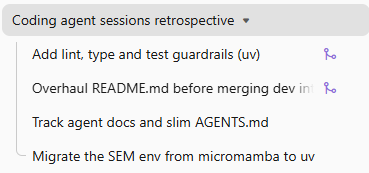
\includegraphics[height=23.4mm]{assets/screens/claude-app-forks.png}};
    \begin{scope}[shift={(shot.south west)},x={($(shot.south east)-(shot.south west)$)},
        y={($(shot.north west)-(shot.south west)$)}]
      \node[number mark] at (0.813,0.879) {1};
      \node[number mark] at (0.043,0.387) {2};
      \node[number mark] at (0.954,0.682) {3};
    \end{scope}
    \foreach \t [count=\k] in {one session,{its forks, one per task},pull request merged} {
      \node[number mark] at (56.4,-33.6-\k*6.6+6.6) {\k};
      \node[key] at (59.6,-33.6-\k*6.6+6.6) {\t};
    }
    \fill[termbg,rounded corners=1.2mm] (100,-31.4) rectangle (144,-45.6);
    \foreach \c [count=\i] in {termdot1,termdot2,termdot3} \fill[\c] (100.4+\i*2.3,-34) circle (0.7);
    \node[inner sep=0pt,font=\ttfamily\fontsize{7}{8}\selectfont,text=termdim] at (124.6,-34)
      {second terminal};
    \draw[white!18!termbg,line width=0.4pt] (100,-36.6) -- (144,-36.6);
    \node[mono,text=termfg] at (102.4,-39.6) {\textcolor{termgreen}{\$} claude -c --fork-session};
    \node[mono,text=termfg] at (102.4,-43) {> work in a worktree};
    \node[anchor=north west,inner sep=0pt,font=\scriptsize,text=udsgrey] at (100,-47.4)
      {forks the latest session in this folder};
  \end{tikzpicture}
  \note{\textbf{24:00--24:50}\par
    A tip from daily use: a session often turns into more than one task.\par
    Fork it with slash fork rather than start again: each fork keeps the whole conversation, the
      plan and the decisions included.\par
    Then ask each fork to work in a worktree; Claude Code creates one under .claude/worktrees and
      moves the session into it.\par
    Until then both forks work in the same folder, and their edits can collide.\par
    In the app the forks sit under their session in the sidebar: here four tasks that came out of
      one session, each in its own worktree; purple marks a merged pull request.\par
    In a terminal, slash fork copies the conversation into a new session and keeps you in this
      one; from a second terminal, claude with continue and fork-session copies the latest session
      of the folder.}
\end{frame}

\section[Tests first]{Tests first}
\sectionframe{06}{Tests first}
  {How does a test written before the code keep an agent on track?}
  {\faCheckDouble}

% ---------------------------------------------------------------- the loop
\begin{frame}[source={Beck (2002), Test-Driven Development: By Example}]{Test-Driven Development (TDD)}
  \begin{tikzpicture}[x=1mm,y=1mm,
      phase/.style={box,text width=28mm,minimum height=13mm,font=\footnotesize,line width=0.8pt},
      gain/.style={inner sep=0pt,font=\footnotesize,text=udsdark,align=left},
      tick/.style={inner sep=0pt,font=\footnotesize,anchor=base east}]
    \useasboundingbox (0,-1.36) rectangle (144,-55);
    \node[phase,draw=udsred,fill=redtint] (red) at (72,-8)
      {{\color{udsred}\bfseries\small RED}\\[0.4mm] write a failing test for one behaviour};
    \node[phase,draw=testgreen,fill=greentint] (green) at (96,-40)
      {{\color{testgreen}\bfseries\small GREEN}\\[0.4mm] write just enough code to pass it};
    \node[phase,draw=udsblue,fill=bluetint] (ref) at (48,-40)
      {{\color{udsblue}\bfseries\small REFACTOR}\\[0.4mm] tidy the code; every test stays green};
    \draw[flow] (red.east) to[bend left=35] (green.north);
    \draw[flow] (green.west) -- (ref.east);
    \draw[flow] (ref.north) to[bend left=35] (red.west);
    \node[lbl,align=center] at (72,-27) {one behaviour\\per cycle};
    % what each step gives us; each tick sits on its gain's first baseline (with a text width,
    % a node's base is its first line); the two gains of RED start at x = 98, clear of the arrow
    % from RED to GREEN
    \node[gain,anchor=west] (g1) at (98,-5.2) {the requirement, written first};
    \node[gain,anchor=west] (g2) at (98,-10.8) {proof that the test can fail};
    \node[gain,anchor=west,text width=20mm] (g3) at (118.4,-40) {small steps,\\easy to review};
    \node[gain,anchor=west,text width=22mm] (g4) at (8,-40) {a regression net\\for later changes};
    \foreach \g/\c in {g1/udsred,g2/udsred,g3/testgreen,g4/udsblue}
      \node[tick,text=\c] at ([xshift=-1.4mm]\g.base west) {\faCheck};
    \node[gain,anchor=base] (g5) at (74,-53.4) {tests call clear interfaces: the seams};
    \node[tick,text=udsdark] at ([xshift=-1.4mm]g5.base west) {\faCheck};
  \end{tikzpicture}
  \note{\textbf{25:00--26:00}\par
    Test-driven development in Kent Beck's formulation is a short loop.\par
    Red: write a test for one behaviour and watch it fail.\par
    Green: write just enough code to make it pass.\par
    Refactor: tidy the code while all tests stay green.\par
    Then the next behaviour.\par
    What we get: the requirement written down as a test before the code exists, proof that each
      test can fail, small steps, a regression net, and pressure towards clear interfaces, the
      seams where tests observe behaviour.}
\end{frame}

% ------------------------------------------------------- why for an agent
\begin{frame}[source={Anthropic (2026), Claude Code best practices · Mathews \& Nagappan (2024), ASE ’24}]{Why tests first help an agent}
  \begin{tikzpicture}[x=1mm,y=1mm,
      node2/.style={box,minimum height=9mm,inner sep=1.6mm},
      item/.style={anchor=base west,inner sep=0pt,font=\footnotesize,text=udsdark},
      head/.style={anchor=base west,inner sep=0pt,font=\footnotesize\bfseries}]
    \useasboundingbox (0,0) rectangle (144,-54);
    % the agent edits the code and runs the tests
    \node[node2,artifact,font=\ttfamily\footnotesize\bfseries,minimum width=20mm] (src) at (12,-8) {src/};
    \node[node2,agent,font=\footnotesize\bfseries,minimum width=26mm] (ag) at (62,-8) {\faRobot\enspace agent};
    \node[node2,artifact,draw=testgreen,fill=greentint,font=\ttfamily\footnotesize\bfseries,minimum width=20mm]
      (tst) at (114,-8) {tests/};
    \draw[flow] (ag.west) -- node[lbl,above] {edits} (src.east);
    \draw[flow] (ag.east) -- node[lbl,above] {runs} (tst.west);
    \node[anchor=south,inner sep=0pt,font=\scriptsize,text=testgreen] at ([yshift=1mm]tst.north)
      {\faLock\enspace approved and committed first};
    % pass or fail comes back: the signal
    \draw[flow,draw=testgreen,line width=0.8pt] (tst.south) to[out=-90,in=-90,looseness=0.55]
      node[pos=0.5,below,inner sep=0.8mm,font=\scriptsize\bfseries,text=testgreen] {pass or fail} (ag.south);
    % what the signal gives the agent
    \node[head,text=testgreen] at (0,-28.4) {what it gives the agent};
    \foreach \t [count=\i] in {a check it runs itself,{the intent, fixed first},one small goal per cycle,
        earlier decisions still enforced}
      \node[item] at (0,-28.4-\i*4.7) {\textcolor{testgreen}{\faCheck}\enspace\t};
    % how it gets gamed: aimed at the tests, and what catches it
    \node[head,text=udsred] (gamed) at (70,-28.4) {how it gets gamed};
    \foreach \t [count=\i] in {tests edited or skipped,expected values copied from the code,
        a mock that replaces the logic,tests fitted after the code}
      \node[item] at (70,-28.4-\i*4.7) {\textcolor{udsred}{\faTimes}\enspace\t};
    \draw[udsred,line width=0.6pt,dashed,-{Stealth[length=1.7mm,width=1.3mm]}]
      ([xshift=1.5mm]gamed.east) to[out=0,in=-90] (121,-12.6);
    \node[item,text=udsblue] at (70,-53)
      {caught by: test diffs reviewed first · you rerun every test};
  \end{tikzpicture}
  \note{\textbf{26:00--27:00}\par
    Anthropic's guidance for Claude Code puts it plainly: without a check it can run, an agent
      stops when the work looks done.\par
    A failing test turns done into a signal the agent reads and iterates on.\par
    Written first, from the spec, the test records intent instead of mirroring the
      implementation, and the suite keeps earlier decisions enforced in later sessions.\par
    The failure modes are real: agents weaken, skip or edit tests, recompute expected values the
      way the code does, or replace the logic under test with a mock, a stand-in that returns
      whatever the test expects.\par
    Hence our guardrails: read the changes to the tests first, and rerun every test yourself
      rather than trust the agent's report.\par
    A benchmark study found that giving the model the tests with the task solved more problems;
      that is evidence for code generation, not for research code.}
\end{frame}

\section[Workflow]{Skills and an end-to-end workflow}
\sectionframe{07}{Skills and an end-to-end workflow}
  {How does a request become a reviewed change?}
  {\faProjectDiagram}

% ------------------------------------------------------------ what a skill is
% a lab protocol beside a skill file, row for row: what it is called, when to use it, the steps
\begin{frame}[source={Pocock (2026), mattpocock/skills v1.3.1: tdd · agentskills.io, Specification}]{A skill: a lab protocol for the agent}
  \begin{tikzpicture}[x=1mm,y=1mm,
      head/.style={anchor=north west,inner sep=0pt,font=\small\bfseries,text=udsdark},
      prot/.style={anchor=base west,inner sep=0pt,font=\footnotesize,text=udsdark},
      code/.style={anchor=base west,inner sep=0pt,font=\ttfamily\fontsize{7.2}{8.4}\selectfont,text=udsdark},
      num/.style={circle,fill=udsblue,text=white,inner sep=0pt,minimum size=3.6mm,
        font=\fontsize{7}{7}\selectfont\bfseries},
      pair/.style={udsgreymid,line width=0.5pt,dash pattern=on 1pt off 1pt},
      key/.style={fill=white,inner xsep=0.8mm,inner ysep=0.3mm,font=\scriptsize,text=udsgrey},
      say/.style={anchor=north west,inner sep=0pt,font=\scriptsize,text=udsdark}]
    \useasboundingbox (0,0) rectangle (144,-55);
    \node[head] at (0,0) {In the lab\enspace{\mdseries\color{udsgrey}a protocol}};
    \node[head] at (76,0) {In the repository\enspace{\mdseries\color{udsgrey}a skill}};
    % the protocol: a sheet on a clipboard
    \draw[udsgreylight,fill=white,line width=0.5pt,rounded corners=1.2mm] (0,-5.6) rectangle (62,-43.6);
    \fill[udsgreymid,rounded corners=0.8mm] (24,-4.3) rectangle (38,-7.1);
    \node[prot,font=\footnotesize\bfseries] at (3,-14.6) {Sample preparation};
    \node[prot,text=udsgrey] at (3,-18.6) {Use when: a specimen goes to the SEM.};
    \foreach \t [count=\i] in {Grind.,Polish.,Etch.,Check under the light microscope.} {
      \pgfmathsetmacro\y{-29-(\i-1)*4}
      \node[num] at (4.8,\y+0.95) {\i};
      \node[prot] at (8.4,\y) {\t};
    }
    % the skill: its SKILL.md in a file window, as on the slides of section 3
    \node[anchor=north west,inner xsep=1.8mm,inner ysep=0.8mm,text height=1.9mm,text depth=0.6mm,
      font=\ttfamily\fontsize{7}{8}\selectfont,text=udsdark] (tab) at (76,-5.6)
      {\textcolor{udsblue}{\faIcon[regular]{file-alt}}\enspace tdd/SKILL.md\enspace
       \textcolor{udsgreymid}{\sffamily\scriptsize shortened}};
    \begin{scope}
      \clip[rounded corners=1.2mm] (76,-5.6) rectangle (144,-43.6);
      \fill[darktint] (tab.north east) rectangle (144,-9.7);
      \draw[udsblue,line width=0.9pt] (tab.north west) -- (tab.north east);
    \end{scope}
    \draw[udsgreylight,line width=0.5pt,rounded corners=1.2mm] (76,-5.6) rectangle (144,-43.6);
    \node[code] at (78.8,-14.6) {name: tdd};
    \node[code] at (78.8,-18.6) {description: Test-driven development. Use when};
    \node[code] at (78.8,-21.6) {\phantom{xx}the user wants to build features or fix};
    \node[code] at (78.8,-24.6) {\phantom{xx}bugs test-first, ...};
    \foreach \t [count=\i] in {Agree the seams to test.,Write one failing test.,
        Write just enough code to pass.,Repeat for the next behaviour.}
      \node[code] at (78.8,{-29-(\i-1)*4}) {\i. \t};
    % what matches what, the word on its line
    \foreach \y/\k in {-13.7/name,-17.7/when,-34.6/steps} {
      \draw[pair] (63.2,\y) -- (74.8,\y);
      \node[key] at (69,\y) {\k};
    }
    \node[say] at (0,-44.8) {written once; everyone in the lab follows it};
    \node[say] at (76,-44.8) {written once; the agent follows it when needed};
    % when a skill is worth writing, in a strip like the one of slide 5, 2 mm below the captions
    \fill[bluetint] (0,-49.6) rectangle (144,-55);
    \fill[udsblue] (0,-49.6) rectangle (1.2,-55);
    \node[anchor=west,inner sep=0pt,font=\footnotesize,text=udsdark] at (3.6,-52.3)
      {\textcolor{udsblue}{\faClipboardList}\enspace one procedure per kind of task};
    \node[anchor=west,inner sep=0pt,font=\footnotesize,text=udsdark] at (74,-52.3)
      {\textcolor{udsblue}{\faRedo}\enspace worth writing when the task recurs};
  \end{tikzpicture}
  \note{\textbf{27:10--28:10}\par
    Section 3 gave the agent facts about the repository; a skill gives it a procedure.\par
    It works like a lab protocol: a name, when to use it, and the steps, written once and
      followed by whoever does the task.\par
    A skill is the same for an agent: a Markdown file, here a shortened version of Pocock's
      test-driven development skill.\par
    Without one, we type the same instructions into every prompt, a little differently each
      time.\par
    Written once, the procedure is kept with the project, reviewed like code and improved in one
      place.\par
    Worth it for a task that recurs; a one-off task needs only a good prompt.}
\end{frame}

% ------------------------------------------------------------ inside a skill
\begin{frame}[fragile,source={Pocock (2026), mattpocock/skills v1.3.1: tdd · agentskills.io, Specification · Anthropic (2026), Claude Code docs: Skills · OpenAI (2026), Build skills}]{A skill: procedures loaded when needed}
  \begin{columns}[T,onlytextwidth]
    \begin{column}{0.57\textwidth}
\begin{codefile}[basicstyle=\ttfamily\fontsize{7}{8.4}\selectfont]{tdd/SKILL.md\enspace\textcolor{udsgreymid}{\sffamily\scriptsize shortened}}
---
name: tdd
description: Test-driven development. Use when the user
  wants to build features or fix bugs test-first,
  mentions "red-green-refactor", or wants integration
  tests.
---
# Test-Driven Development
## What a good test is
Tests verify behavior through public interfaces, not
implementation details. ...
See [tests.md](tests.md) for examples and
[mocking.md](mocking.md) for mocking guidelines.
\end{codefile}
      % where the skill folders go, under the file and flush with it
      {\scriptsize\color{udsgrey}\textcolor{udsblue}{\faFolderOpen}\enspace\fn{.claude/skills/} (Claude Code),
       \fn{.agents/skills/} (Codex)\par}
    \end{column}
    \begin{column}{0.4\textwidth}
      % one bracket per part of the file, level with its lines; y = 0 is the top of the file window
      \begin{tikzpicture}[x=1mm,y=1mm,
          what/.style={anchor=west,inner sep=0pt,font=\footnotesize,text=udsdark,align=left,text width=52mm,
            execute at begin node={\hyphenpenalty=10000\raggedright}}]
        \useasboundingbox (0,0) rectangle (57.6,-54);
        \def\first{6.6}\def\pitch{2.952}% the first line's top below the window's top, and the line pitch
        \foreach \a/\b/\t in {1/7/{\textcolor{udsblue}{\bfseries from the start}, like \fn{AGENTS.md}\\
              the name and description of every skill},
            8/11/{\textbf{when it runs}\\ \fn{/tdd}, or a task that matches},
            12/13/{\textbf{when the steps need them}\\ \fn{tests.md}, \fn{mocking.md} in the same folder}} {
          \pgfmathsetmacro\ya{-\first-(\a-1)*\pitch-0.5}
          \pgfmathsetmacro\yb{-\first-\b*\pitch+0.5}
          \draw[udsgreymid,line width=0.6pt] (0,\ya) -- (1.4,\ya) -- (1.4,\yb) -- (0,\yb);
          \node[what] at (3.6,{(\ya+\yb)/2}) {\t};
        }
      \end{tikzpicture}
    \end{column}
  \end{columns}
  \note{\textbf{28:10--29:20}\par
    Technically, a skill is a folder with a SKILL.md file and, where needed, more files beside
      it.\par
    The file starts with a name and a description, which says what the skill is for and when to
      use it.\par
    At the start of a session the agent sees only these lines, for every installed skill, about a
      hundred tokens each, just as it always sees AGENTS.md.\par
    The rest of the file loads when the skill runs: when we type its name, here /tdd, or when the
      agent finds that a task matches the description.\par
    Files beside it, here examples of good tests and rules for mocks, are read only when the
      steps call for them; this is called progressive disclosure.\par
    Committed with the code, the skill reaches everyone who works in the repository.}
\end{frame}

% ------------------------------------------------------------ the collection
\begin{frame}[source={Pocock (2026), mattpocock/skills v1.3.1: README · github.com/mattpocock/skills, 20 Oct 2026}]{Matt Pocock's skills: an end-to-end workflow}
  \begin{columns}[T,onlytextwidth]
    \begin{column}{0.56\textwidth}
      % the repository's address, which the screenshot's crop leaves out, as a link
      {\footnotesize\href{https://github.com/mattpocock/skills}{\faGithub\enspace\underline{\fn{mattpocock/skills}}}\par}
      \vskip1.6mm
      \begin{tikzpicture}
        \node[anchor=south west,inner sep=0pt,draw=udsgreylight,line width=0.4pt] (img) at (0,0)
          {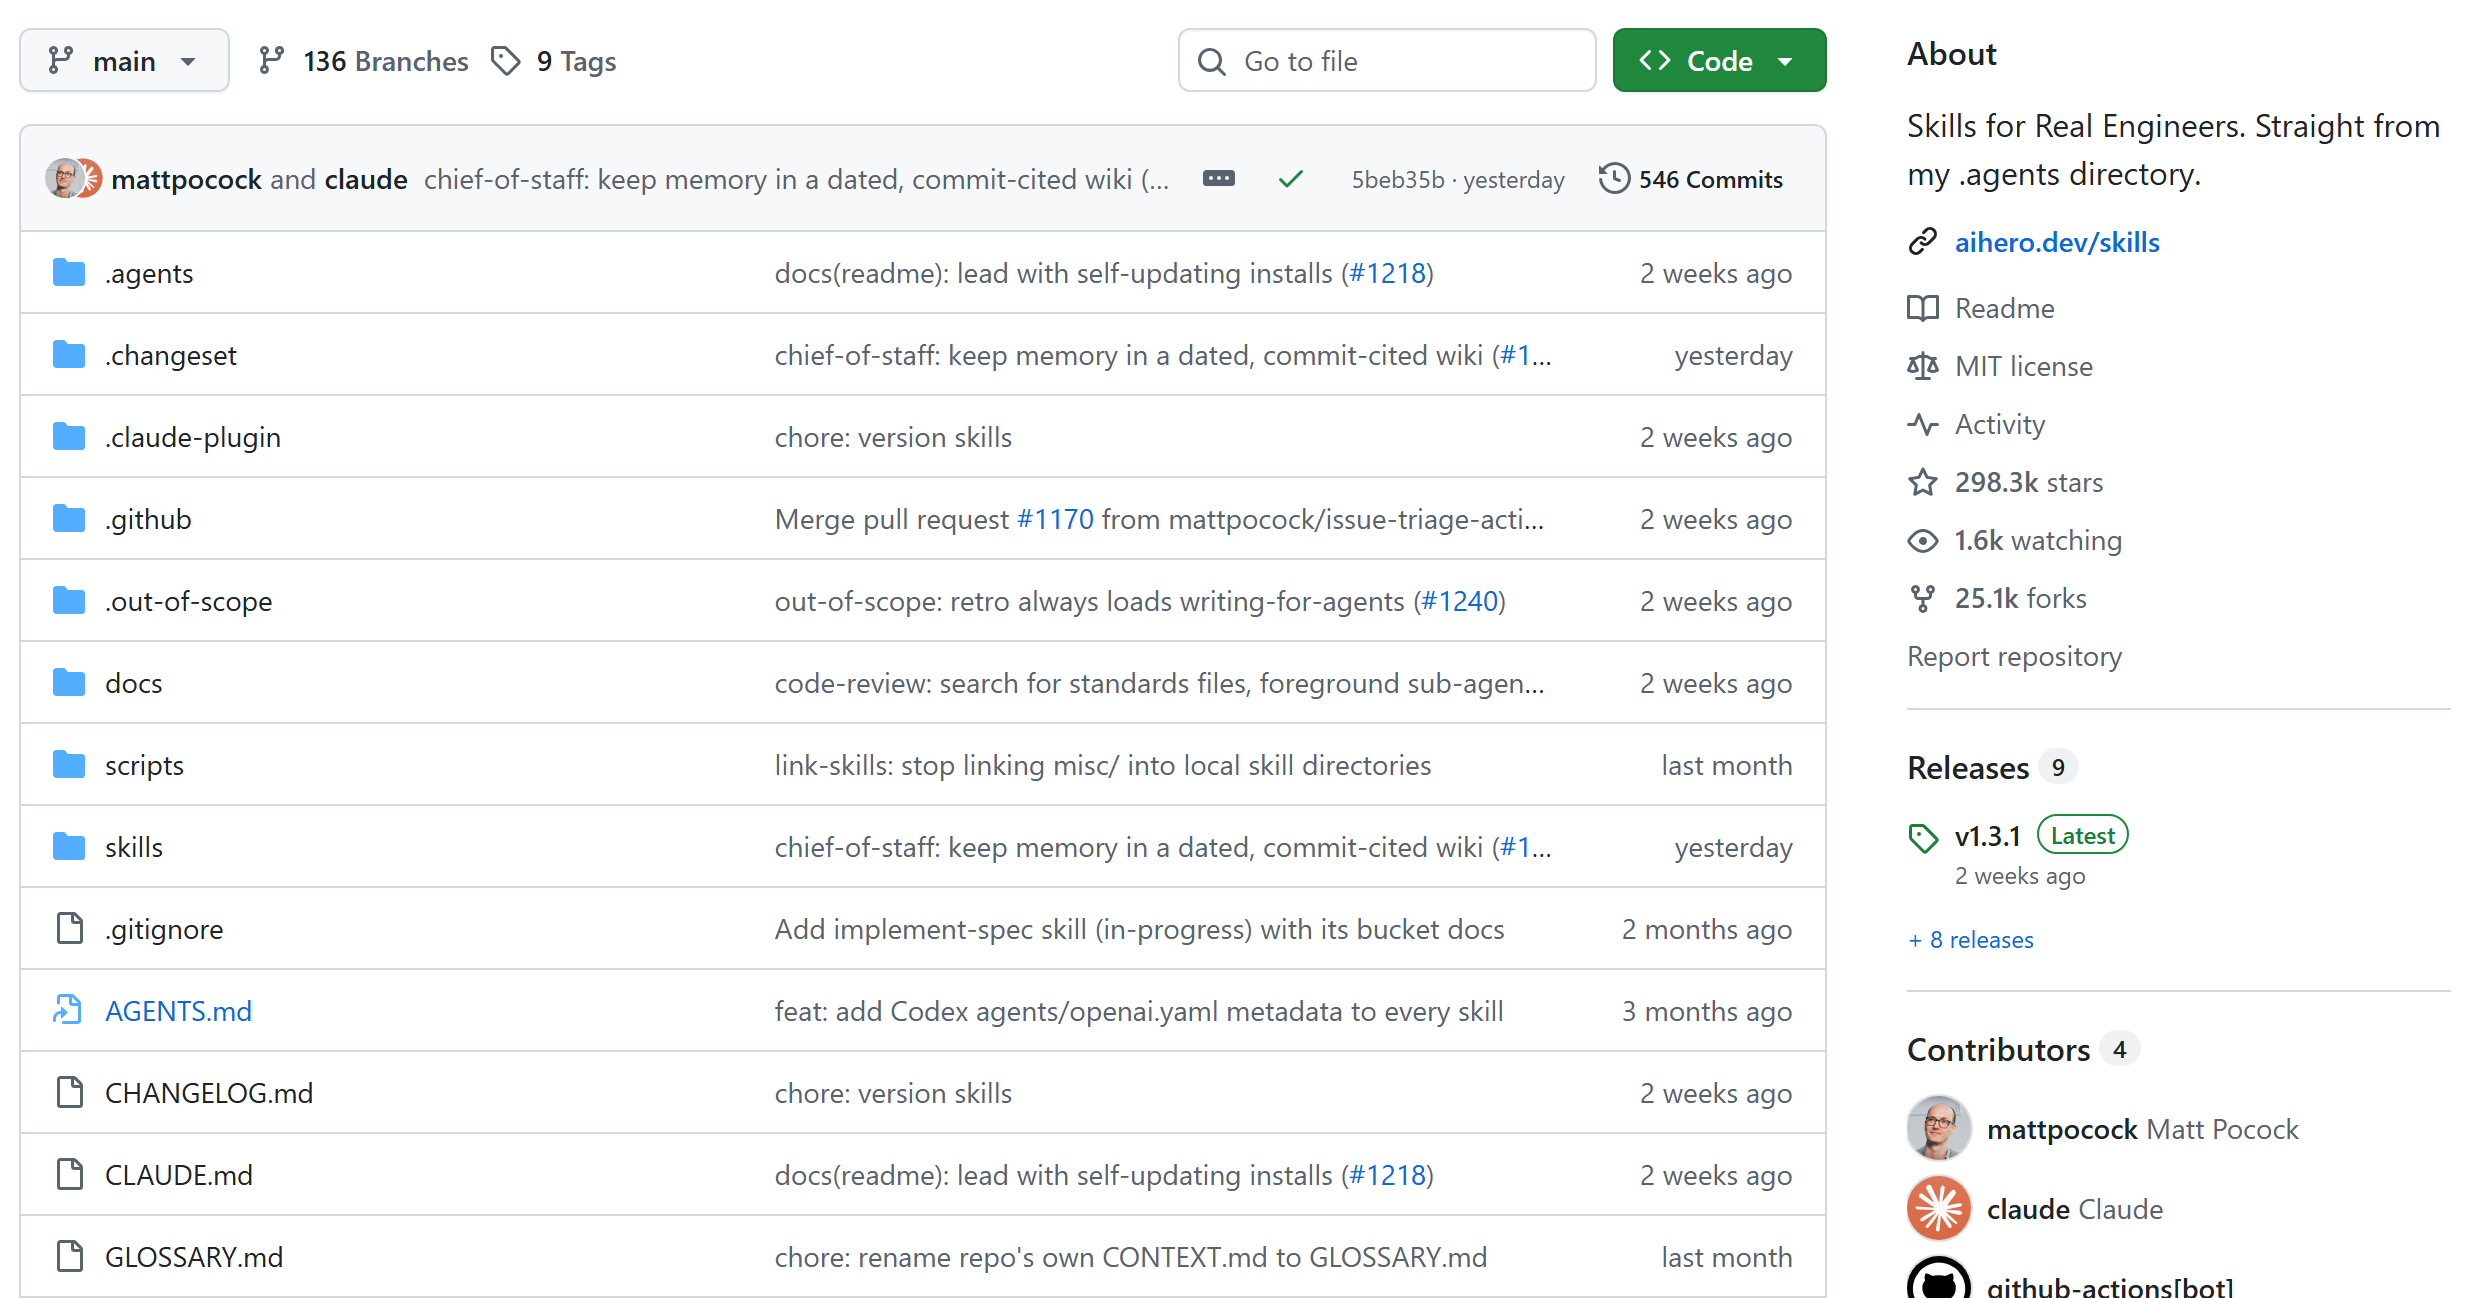
\includegraphics[width=\linewidth]{assets/screens/github-skills.png}};
        \begin{scope}[x={(img.south east)},y={(img.north west)},udsred,line width=1.1pt]
          \draw (0.014,0.320) rectangle (0.077,0.374);
          \draw (0.014,0.193) rectangle (0.109,0.247);
          \draw (0.014,0.005) rectangle (0.123,0.058);
          \draw (0.766,0.333) rectangle (0.871,0.386);
        \end{scope}
      \end{tikzpicture}
    \end{column}
    \begin{column}{0.41\textwidth}
      % two kinds of skill: the ones you type run a stage, and call the ones the agent may also pick
      \begin{tikzpicture}[x=1mm,y=1mm,
          kind/.style={anchor=north west,inner sep=0pt,font=\footnotesize\bfseries},
          chip/.style={anchor=west,minimum height=4.6mm,inner xsep=1mm,inner ysep=0pt,line width=0.5pt,
            font=\ttfamily\fontsize{7}{8}\selectfont,text=udsdark},
          you/.style={chip,draw=udsred,fill=redtint,minimum width=23.6mm},
          it/.style={chip,draw=udsblue,fill=bluetint,minimum width=22mm},
          call/.style={-{Stealth[length=1.5mm,width=1.1mm]},line width=0.5pt,draw=udsdark},
          say/.style={anchor=north west,inner sep=0pt,font=\scriptsize,text=udsgrey}]
        \useasboundingbox (0,0) rectangle (59,-54);
        \node[kind,text=udsred] at (0,0) {\faUser\enspace you type};
        \node[kind,text=udsblue] at (31,0) {\faRobot\enspace the agent may use};
        \foreach \s [count=\i from 0] in {/grill-with-docs,/to-spec,/to-tickets,/implement}
          \node[you] (u\i) at (0,{-7.6-\i*6.4}) {\s};
        \foreach \s [count=\i from 0] in {domain-modeling,codebase-design,tdd,code-review}
          \node[it] (m\i) at (31,{-7.6-\i*6.4}) {\s};
        % who calls whom, as the SKILL.md files say
        \draw[call] (u0.east) -- (m0.west);
        \draw[call] (u3.east) -- (m2.west);
        \draw[call] (u3.east) -- (m3.west);
        \draw[call] (m2.east) to[out=0,in=0,looseness=1.6] (m1.east);
        \node[say] at (0,-31.6) {each runs one stage};
        \node[say] at (31,-31.6) {rules and vocabulary};
        % installing: the files are copied into the project
        \fill[termbg,rounded corners=1mm] (0,-37) rectangle (57,-45.8);
        \foreach \c [count=\i] in {termdot1,termdot2,termdot3} \fill[\c] (\i*2.3,-39.2) circle (0.7);
        \node[inner sep=0pt,font=\ttfamily\fontsize{7}{8}\selectfont,text=termdim] at (28.5,-39.2) {install};
        \node[anchor=west,inner sep=0pt,font=\ttfamily\fontsize{7}{8}\selectfont,text=termfg] at (1.8,-43.4)
          {\textcolor{termgreen}{\$} npx skills@latest add mattpocock/skills};
        \node[say,text=udsred] at (0,-47.6) {\faExclamationTriangle\enspace read them first};
      \end{tikzpicture}
    \end{column}
  \end{columns}
  \note{\textbf{29:20--30:10}\par
    Our example is Matt Pocock's open-source collection on GitHub; the repository uses its own
      AGENTS.md and GLOSSARY.md.\par
    Its skills come in two kinds: the ones we type each run one stage of the work, and they call
      skills that the agent may also pick up by itself, which hold the rules.\par
    Grill-with-docs calls domain-modeling, implement calls tdd and code-review, and tdd looks up
      codebase-design for its vocabulary.\par
    The installer copies the files into the project; skills are instructions and scripts written
      by someone else, so read them before the agent uses them.}
\end{frame}

% ------------------------------------------------------- the books behind
% \bookcover{x}{colour}{title}{author}{year}: a book seen from the front, 22 x 27 mm, its top-left
% corner at (x,0); the darker strip on the left is the spine
\newcommand\bookcover[5]{%
  \begin{scope}
    \clip[rounded corners=0.9mm] (#1,0) rectangle ++(22,-27);
    \fill[#2] (#1,0) rectangle ++(22,-27);
    \fill[black,opacity=0.22] (#1,0) rectangle ++(1.9,-27);
  \end{scope}
  \node[anchor=north west,inner sep=0pt,text width=17.6mm,align=left,font=\scriptsize\bfseries,
    text=white,execute at begin node={\hyphenpenalty=10000\raggedright}] at (#1+3,-2.6) {#3};
  \node[anchor=south west,inner sep=0pt,text width=17.6mm,align=left,font=\scriptsize,
    text=white!80!#2] at (#1+3,-2.4-22.2) {#4\\#5};}
\begin{frame}[source={Hunt \& Thomas (1999) · Beck (1999; 2002) · Fowler (1999) · Evans (2003) · Ousterhout (2018) · Pocock (2026), mattpocock/skills v1.3.1: README, code-review, codebase-design}]{Classic practice, adapted for agents}
  % each book, the idea the skills take from it, and the skills that carry it
  \begin{tikzpicture}[x=1mm,y=1mm,
      idea/.style={anchor=north west,inner sep=0pt,text width=22mm,align=left,font=\scriptsize,
        text=udsdark,execute at begin node={\hyphenpenalty=10000\raggedright}},
      sk/.style={spec skill},
      fl/.style={spec chip}]
    \useasboundingbox (0,0) rectangle (144,-54);
    \bookcover{0}{udsdark}{The Pragmatic Programmer}{Andrew Hunt,\\David Thomas}{1999}
    \bookcover{24.4}{udsblue}{Extreme Programming Explained}{Kent Beck}{1999}
    \bookcover{48.8}{udsdark}{Refactoring}{Martin Fowler}{1999}
    \bookcover{73.2}{testgreen}{Test-Driven Development: By Example}{Kent Beck}{2002}
    \bookcover{97.6}{udsblue}{Domain-Driven Design}{Eric Evans}{2003}
    \bookcover{122}{udsdark}{A Philosophy of Software Design}{John\\Ousterhout}{2018}
    \foreach \x/\t in {0/{no one knows exactly what they want},24.4/{user stories; invest in the design every day},
        48.8/{code smells},73.2/{red, green, refactor},97.6/{a ubiquitous language},122/{deep modules}}
      \node[idea] at (\x,-29.4) {\t};
    \node[sk] at (0,-39.6) {/grill-with-docs};
    \node[sk] at (24.4,-39.6) {/to-spec};
    \node[sk] at (48.8,-39.6) {/code-review};
    \node[sk] at (73.2,-39.6) {/tdd};
    \node[fl] at (97.6,-39.6) {GLOSSARY.md};
    \node[sk] at (97.6,-45.2) {/domain-modeling};
    \node[sk] at (122,-39.6) {/codebase-design};
  \end{tikzpicture}
  \note{\textbf{30:10--31:20}\par
    None of this is new: Pocock's README says the skills rest on decades of engineering
      experience, and quotes the books.\par
    The Pragmatic Programmer: no one knows exactly what they want, so the agent asks before it
      builds; its tracer bullets return as the vertical slices of to-tickets.\par
    Kent Beck's Extreme Programming brought the user stories that to-spec writes into every spec,
      and the advice to invest in the design every day.\par
    Fowler's Refactoring catalogues code smells, which code-review looks for in every diff.\par
    Beck's red, green, refactor loop, the subject of section 6, is the tdd skill.\par
    Evans: one ubiquitous language for people and code, our glossary; Ousterhout: deep modules,
      much behaviour behind a small interface.\par
    What is new is the reader: the model has read these books, so a term such as tracer bullets
      or red and green brings the whole practice into a skill in a few words.}
\end{frame}

% Pocock's README, section "Why These Skills Exist", word for word (mattpocock/skills, MIT licence;
% the same on main on 3 November 2026 as in v1.3.1), with its links and the aside on the commit of its example glossary dropped: notes pages of their
% own, outside the frame, so they follow slide 29's notes page and stay out of the audience PDF. A
% note outside a frame does not get the theme's note style, so each one sets it first.
\note{\parindent=0pt\parskip=1.1mm\raggedright\footnotesize
  \textbf{Slide 29, continued (1 of 5): Pocock's README, ``Why These Skills Exist''}\par
  I built these skills as a way to fix common failure modes I see with Claude Code, Codex, and other
    coding agents.\par
  \textbf{\#1: The Agent Didn't Do What I Want}\par
  \emph{``No-one knows exactly what they want''}\enspace--- David Thomas \& Andrew Hunt, The Pragmatic
    Programmer\par
  \textbf{The Problem}. The most common failure mode in software development is misalignment. You think
    the dev knows what you want. Then you see what they've built - and you realize it didn't understand
    you at all.\par
  This is just the same in the AI age. There is a communication gap between you and the agent. The fix
    for this is a \textbf{grilling session} - getting the agent to ask you detailed questions about what
    you're building.\par
  \textbf{The Fix} is to use: \fn{/grill-me} - for non-code uses; \fn{/grill-with-docs} - same as
    \fn{/grill-me}, but adds more goodies (see below).\par
  These are my most popular skills. They help you align with the agent before you get started, and
    think deeply about the change you're making. Use them \emph{every} time you want to make a
    change.}
\note{\parindent=0pt\parskip=1.1mm\raggedright\footnotesize
  \textbf{Slide 29, continued (2 of 5)}\par
  \textbf{\#2: The Agent Is Way Too Verbose}\par
  \emph{``With a ubiquitous language, conversations among developers and expressions of the code are
    all derived from the same domain model.''}\enspace--- Eric Evans, Domain-Driven-Design\par
  \textbf{The Problem}: At the start of a project, devs and the people they're building the software
    for (the domain experts) are usually speaking different languages.\par
  I felt the same tension with my agents. Agents are usually dropped into a project and asked to figure
    out the jargon as they go. So they use 20 words where 1 will do.\par
  \textbf{The Fix} for this is a shared language. It's a document that helps agents decode the jargon
    used in the project.\par
  Example: here's an example glossary, from my \fn{course-video-manager} repo. Which one is easier to
    read? \textbf{BEFORE}: ``There's a problem when a lesson inside a section of a course is made `real'
    (i.e.\ given a spot in the file system)''. \textbf{AFTER}: ``There's a problem with the
    materialization cascade''. This concision pays off session after session.}
\note{\parindent=0pt\parskip=1.1mm\raggedright\footnotesize
  \textbf{Slide 29, continued (3 of 5)}\par
  \textbf{\#2, continued}\par
  This is built into \fn{/grill-with-docs}. It's a grilling session, but that helps you build a shared
    language with the AI, and document hard-to-explain decisions in ADR's.\par
  It's hard to explain how powerful this is. It might be the single coolest technique in this repo.
    Try it, and see.\par
  Tip: a shared language has many other benefits than reducing verbosity: \textbf{variables, functions
    and files are named consistently}, using the shared language; as a result, the \textbf{codebase is
    easier to navigate} for the agent; the agent also \textbf{spends fewer tokens on thinking}, because
    it has access to a more concise language.}
\note{\parindent=0pt\parskip=1.1mm\raggedright\footnotesize
  \textbf{Slide 29, continued (4 of 5)}\par
  \textbf{\#3: The Code Doesn't Work}\par
  \emph{``Always take small, deliberate steps. The rate of feedback is your speed limit. Never take on a
    task that's too big.''}\enspace--- David Thomas \& Andrew Hunt, The Pragmatic Programmer\par
  \textbf{The Problem}: Let's say that you and the agent are aligned on what to build. What happens when
    the agent \emph{still} produces crap?\par
  It's time to look at your feedback loops. Without feedback on how the code it produces actually runs,
    the agent will be flying blind.\par
  \textbf{The Fix}: You need the usual tranche of feedback loops: static types, browser access, and
    automated tests.\par
  For automated tests, a red-green-refactor loop is critical. This is where the agent writes a failing
    test first, then fixes the test. This helps give the agent a consistent level of feedback that
    results in far better code.\par
  I've built a \textbf{\fn{/tdd} skill} you can slot into any project. It encourages red-green-refactor
    and gives the agent plenty of guidance on what makes good and bad tests.\par
  For debugging, I've also built a \textbf{\fn{/diagnosing-bugs}} skill that wraps best debugging
    practices into a disciplined loop, gated phase by phase.}
\note{\parindent=0pt\parskip=1.1mm\raggedright\footnotesize
  \textbf{Slide 29, continued (5 of 5)}\par
  \textbf{\#4: We Built A Ball Of Mud}\par
  \emph{``Invest in the design of the system \emph{every day}.''}\enspace--- Kent Beck, Extreme Programming
    Explained\par
  \emph{``The best modules are deep. They allow a lot of functionality to be accessed through a simple
    interface.''}\enspace--- John Ousterhout, A Philosophy Of Software Design\par
  \textbf{The Problem}: Most apps built with agents are complex and hard to change. Because agents can
    radically speed up coding, they also accelerate software entropy. Codebases get more complex at an
    unprecedented rate.\par
  \textbf{The Fix} for this is a radical new approach to AI-powered development: caring about the design
    of the code.\par
  This is built in to every layer of these skills: \fn{/to-spec} quizzes you about which modules you're
    touching before creating a spec.\par
  And crucially, \fn{/improve-codebase-architecture} surveys a codebase for deepening opportunities and
    hands you the candidates. I recommend running it on your codebase once every few days. It is a
    survey, not a rescue: on a genuinely old codebase it will find real candidates, but it won't
    untangle the mud for you.\par
  \textbf{Summary}: Software engineering fundamentals matter more than ever. These skills are my best
    effort at condensing these fundamentals into repeatable practices, to help you ship the best apps of
    your career. Enjoy.}

% ------------------------------------------------------------ flow diagram
\begin{frame}[source={Pocock (2026), mattpocock/skills v1.3.1}]{Pocock's flow: who does what}
  \begin{tikzpicture}[x=1mm,y=1mm,
      cell/.style={minimum width=24.4mm,text width=23.2mm,inner sep=0.6mm,align=center,
        execute at begin node={\hyphenpenalty=10000}},
      hcell/.style={cell,human,minimum height=9.6mm,font=\fontsize{7}{8}\selectfont},
      acell/.style={cell,agent,minimum height=17mm,font=\fontsize{7}{8}\selectfont},
      fcell/.style={cell,artifact,minimum height=7.6mm,font=\ttfamily\fontsize{7}{8}\selectfont},
      lane/.style={font=\fontsize{7}{8}\selectfont\bfseries,rotate=90,anchor=center,inner sep=0pt}]
    \node[lane,text=udsred]  at (3,-4.8)  {PERSON};
    \node[lane,text=udsblue] at (3,-23.5) {AGENT};
    \node[lane,text=udsdark] at (3,-39)   {OUTPUT};
    \foreach \skill/\act/\who/\res [count=\k from 0] in {
        grill-with-docs/{questions in rounds; updates the glossary}/{answer; settle the open points}/{GLOSSARY.md, ADR draft},
        to-spec/{writes the spec from the conversation}/{approve scope and acceptance}/{spec (file or issue)},
        to-tickets/{vertical slices, in order}/{approve slices and order}/{ticket files},
        implement/{drives /tdd at the agreed seams; runs the review; commits}/{confirm test seams; rerun the tests}/{code + tests, one commit},
        code-review/{standards and spec, in parallel; proposes refactoring}/{judge findings; review the science}/{report (in session)}} {
      \pgfmathsetmacro\x{20+\k*27.6}
      \node[hcell] (h\k) at (\x,-4.8) {\who};
      \node[acell] (a\k) at (\x,-23.5) {{\ttfamily\bfseries/\skill}\\[0.3mm]\act};
      \node[fcell] (f\k) at (\x,-39) {\res};
      % two-way: the person both steers the stage and decides on its output
      \draw[flow,{Stealth[length=1.7mm,width=1.3mm]}-{Stealth[length=1.7mm,width=1.3mm]},draw=udsred]
        (h\k.south) -- (a\k.north);
      \draw[flow] (a\k.south) -- (f\k.north);
    }
    \foreach \k [evaluate=\k as \n using int(\k+1)] in {0,...,3} \draw[flow,draw=udsblue] (a\k.east) -- (a\n.west);
    \node[artifact,anchor=north west,minimum width=134.6mm,minimum height=5mm,font=\scriptsize,inner sep=0.6mm]
      (ctx) at (7.8,-45.4) {read along the way:\enspace \texttt{AGENTS.md}\enspace\textperiodcentered\enspace
      \texttt{GLOSSARY.md}\enspace\textperiodcentered\enspace\texttt{docs/adr/}\enspace\textperiodcentered\enspace
      \texttt{CODING\_STANDARDS.md} (review)\enspace\textperiodcentered\enspace tests};
    \foreach \a/\b/\t in {7.8/87.4/{one session: clarify, specify, slice},
                          90.6/142.4/{a fresh session per ticket}} {
      \draw[udsgreymid,line width=0.5pt] (\a,-52.5) -- ++(0,-1.2) -- (\b,-53.7) -- ++(0,1.2);
      \node[lbl,anchor=north] at ({(\a+\b)/2},-54.1) {\t};
    }
  \end{tikzpicture}
  \note{\textbf{31:20--32:30}\par
    The main flow as the author documents it: clarify with grill-with-docs, write the spec, cut
      tickets, implement each ticket.\par
    In today's terms this is spec-driven development: an approved spec before any code, then each
      ticket built test-first.\par
    Tickets are vertical slices: each a thin path through the whole program, from the command
      line to the output, usable on its own.\par
    Implement drives the tdd skill at the test seams agreed in the spec, the public functions
      and command-line options that the tests call; then it runs code-review and commits.\par
    Code-review checks the repository's coding standards and the spec, and is where refactoring
      is proposed.\par
    Red marks the decisions that stay with us at every stage.\par
    The author's context advice: one session from clarification to tickets, then a fresh session
      per ticket that starts from the written ticket.}
\end{frame}

% ---------------------------------------------------- a grilling session
% \sessiondot{n}: the theme's \numbermark, 3.6 mm across; \sessionmark{n} is the same without height, so a
% marker on a session line does not move the lines around it
\newcommand\sessiondot[1]{\tikz[baseline=-0.75ex]\node[circle,fill=udsred,text=white,inner sep=0pt,
  minimum size=3.6mm,font=\sffamily\fontsize{7}{7}\selectfont\bfseries] {#1};}
\newcommand\sessionmark[1]{\smash{\sessiondot{#1}}}
% \sessionarrow{text}: a session line, then an arrow from its end across the column gap to the
% window in the right column; drawn inside the frame, so the notes thumbnail shows it too. The
% terminal's text sits 3.2 mm inside its right edge (1 mm box separation plus 2.2 mm padding).
\newcommand\sessionarrow[1]{%
  \setbox0\hbox{\setbox2\hbox{x}\spaceskip=\wd2 #1}\copy0
  \edef\sessionarrowend{\the\dimexpr\linewidth+3.2mm+\colgap-\wd0+0.1mm\relax}%
  \tikz[overlay,baseline=0pt]\draw[udsred,line width=0.8pt,-{Stealth[length=2mm,width=1.6mm]}]
    (1.4mm,0.9mm) -- (\sessionarrowend,0.9mm);}
\begin{frame}[fragile,source={Pocock (2026), mattpocock/skills v1.3.1: grill-with-docs, grilling, domain-modeling}]{A \texttt{/grill-with-docs} session}
  % the gap between the columns, which the glossary arrow crosses
  \edef\colgap{\the\dimexpr0.03\textwidth\relax}
  \begin{columns}[T,onlytextwidth]
    \begin{column}{0.61\textwidth}
\begin{terminal}[basicstyle=\ttfamily\fontsize{7}{8}\selectfont]{example session}
> /grill-with-docs Add validation folds by specimen to the
  training CLI, as decided in ADR-0003.
§\textcolor{termred}{\smash{\faQuestionCircle}}§ §\textbf{Q1 Default number of folds}§: the manifest lists §\sessionmark{1}§
  three specimens. One fold per specimen?
§\textcolor{termblue}{\smash{\faArrowRight}}§ Yes: k = number of specimens; --folds can lower it. §\sessionmark{2}§

§\textcolor{termred}{\smash{\faQuestionCircle}}§ §\textbf{Q2 What validation claims}§: each specimen is the only
  one of its material state, a term GLOSSARY.md lacks.
  Report folds as unseen material states, and add it?
§\textcolor{termblue}{\smash{\faArrowRight}}§ Yes.

§\textcolor{termred}{\smash{\faQuestionCircle}}§ §\textbf{Q3 Rows without specimen\_id}§: stop with a ValueError,
  as CODING_STANDARDS.md asks?
§\textcolor{termblue}{\smash{\faArrowRight}}§ Yes, and name the rows in the message.
> yes to all
§\sessionarrow{Updated GLOSSARY.md: Material state.}§
No ADR: the number of folds is easy to change later. §\sessionmark{3}§
\end{terminal}
    \end{column}
    \begin{column}{0.36\textwidth}
      % the legend on top; the glossary window at the bottom, level with the line that updates it
      \begin{minipage}[t][58mm][t]{\linewidth}
        \footnotesize
        \begin{tabular}{@{}c@{\enspace}l@{}}
          \sessiondot{1} & a fact the agent looked up\\[1.4mm]
          \sessiondot{2} & a recommended answer\\[1.4mm]
          \sessiondot{3} & an ADR only if hard to reverse\\
        \end{tabular}
        \vfill
\begin{codefile}[basicstyle=\ttfamily\fontsize{7}{8}\selectfont]{GLOSSARY.md\enspace\textcolor{udsgreymid}{new entry}}
Material state: the processing
  condition of a specimen (AsCast,
  Q980_0h_WC, Q980_9h_AC); here,
  one specimen per state.
\end{codefile}
        \vspace{-2.2mm}% the box's own skip below it, so its bottom meets the terminal's
      \end{minipage}
    \end{column}
  \end{columns}
  \note{\textbf{32:30--33:50}\par
    What grilling looks like on our request; the session is abridged and written for our example
      in the format of Pocock's skills.\par
    Each round asks every question that can be asked now, numbered, each with a recommended
      answer (2), worded so that yes accepts it.\par
    The agent looks up facts itself, here the number of specimens in the manifest (1), and
      leaves the decisions to us.\par
    When a term settles, it goes into the glossary at once (the arrow); here the session finds
      that every specimen is also the only one of its material state, which matters for what
      validation can claim.\par
    It offers an ADR only when a decision is hard to reverse, surprising and a real trade-off,
      so the number of folds gets none (3).\par
    Pocock's video of July 2026 shows a full session on his own project.}
\end{frame}

% ------------------------------------------------------------- walkthrough
% \stagefile{node}{x centre}{y top}{tab}{body}: a small file window under a stage, drawn as the
% codefile box is; (node) is its page and (nodet) its tab
\newcommand\stagefile[5]{%
  \node[anchor=north west,inner xsep=1mm,inner ysep=0.7mm,text height=1.9mm,text depth=0.5mm,
    font=\ttfamily\fontsize{7}{8}\selectfont,text=udsdark] (#1t) at (#2-12.2,#3)
    {\textcolor{udsblue}{\faIcon[regular]{file-alt}}\enspace#4};
  \node[anchor=north,minimum width=24.4mm,text width=22mm,inner xsep=1.2mm,inner ysep=1.3mm,
    align=left,font=\ttfamily\fontsize{7}{8.4}\selectfont,text=udsdark] (#1) at (#2,#3-4.2) {#5};
  \begin{scope}
    \clip[rounded corners=1mm] (#2-12.2,#3) rectangle ($(#1.south)+(12.2,0)$);
    \fill[darktint] (#1t.north east) rectangle (#2+12.2,#3-4.2);
    \draw[udsblue,line width=1.4pt] (#1t.north west) -- (#1t.north east);
  \end{scope}
  \draw[udsgreylight,line width=0.5pt,rounded corners=1mm] (#2-12.2,#3) rectangle ($(#1.south)+(12.2,0)$);}
\begin{frame}{The specimen split, stage by stage}
  \begin{tikzpicture}[x=1mm,y=1mm,
      stage/.style={agent,minimum width=24.4mm,minimum height=6.2mm,inner sep=0.6mm,
        font=\ttfamily\bfseries\fontsize{7}{8}\selectfont},
      ticket/.style={draw=udsgreylight,fill=white,line width=0.5pt,anchor=north,minimum width=24.4mm,
        text width=21.4mm,inner xsep=1.5mm,inner ysep=0.9mm,align=left,font=\scriptsize,text=udsdark,
        execute at begin node={\hyphenpenalty=10000\raggedright},
        path picture={\fill[udsdark] (path picture bounding box.north west) rectangle
          ([xshift=0.9mm]path picture bounding box.south west);}},
      say/.style={anchor=north,inner sep=0pt,font=\scriptsize,text=udsgrey,align=center,text width=25mm,
        execute at begin node={\hyphenpenalty=10000}},
      commit/.style={circle,draw=udsblue,fill=white,line width=0.9pt,minimum size=3mm,inner sep=0pt}]
    % an invisible copy of a lane label of "Pocock's flow: who does what" gives this picture the
    % same left edge, so the five columns sit exactly under those of that slide
    \node[font=\fontsize{7}{8}\selectfont\bfseries,rotate=90,anchor=center,inner sep=0pt,opacity=0]
      at (3,-4.8) {PERSON};
    % the short request starts the flow
    \fill[termbg,rounded corners=1mm] (7.8,0) rectangle (142.6,-6.4);
    \foreach \c [count=\i] in {termdot1,termdot2,termdot3} \fill[\c] (7.8+\i*2.3,-3.2) circle (0.7);
    \node[anchor=west,inner sep=0pt,font=\ttfamily\fontsize{7}{8}\selectfont,text=termfg] at (17,-3.2)
      {> Add validation folds by specimen to the training CLI, as decided in ADR-0003.};
    % the five stages, as on "Pocock's flow: who does what"
    \foreach \s [count=\k from 0] in {grill-with-docs,to-spec,to-tickets,implement,code-review}
      \node[stage] (s\k) at (20+\k*27.6,-13.6) {/\s};
    \draw[flow] (20,-6.4) -- (s0.north);
    \foreach \k [evaluate=\k as \n using int(\k+1)] in {0,...,3} \draw[flow,draw=udsblue] (s\k.east) -- (s\n.west);
    \foreach \k in {0,...,4} \draw[flow] (s\k.south) -- ++(0,-3.4);
    % 1: answers, and a new glossary term
    \stagefile{w0}{20}{-21.2}{GLOSSARY.md}{\textcolor{testgreen}{+}\,Material state}
    \node[say] at ([yshift=-1.4mm]w0.south) {Q1 to Q3 answered};
    % 2: the spec
    \stagefile{w1}{47.6}{-21.2}{spec.md}{\textcolor{udsblue}{\bfseries\#\# Decisions}\\
      \textcolor{udsblue}{\bfseries\#\# Test seams}\\ \textcolor{udsblue}{\bfseries\#\# Out of scope}}
    % 3: three vertical slices, each usable on its own
    \node[ticket] (t1) at (75.2,-21.2) {\textbf{T1}\enspace\fn{--split specimen}, end to end};
    \node[ticket] (t2) at ([yshift=-1.4mm]t1.south) {\textbf{T2}\enspace overlap guard and errors};
    \node[ticket] (t3) at ([yshift=-1.4mm]t2.south) {\textbf{T3}\enspace provenance in the fold file};
    % 4: one commit per ticket, each in a fresh session
    \draw[udsblue,line width=1pt] (95.4,-20.4) -- (95.4,-45.6);
    \foreach \t [count=\i from 0] in {T1,T2,T3} {
      \node[commit] (k\i) at (95.4,-24-\i*8.6) {};
      \node[anchor=west,inner sep=0pt,font=\scriptsize,text=udsdark] at ([xshift=1.4mm]k\i.east)
        {\textbf{\t}\enspace tests, code};
    }
    \node[say] at (102.8,-47.6) {a fresh session per ticket};
    % 5: the review report on two axes
    \stagefile{w4}{130.4}{-21.2}{report}{\fontsize{7}{8.4}\sffamily
      \textcolor{udsblue}{\faSearch}\enspace standards\\[0.4mm] \textcolor{udsblue}{\faSearch}\enspace spec}
    \node[say] at ([yshift=-1.4mm]w4.south) {findings for you to judge};
  \end{tikzpicture}
  \note{\textbf{33:50--35:00}\par
    The whole flow on our task, starting from the short request.\par
    Each stage leaves something we can open and check.\par
    Grilling settles what the repository leaves open: the default number of folds, and what
      validation is meant to show with only three specimens.\par
    The spec records the decisions and the test seams.\par
    Tickets are thin vertical slices, each usable on its own: first the whole path from the
      command line to a fold file, then the overlap guard and the error cases, then the
      provenance stored in the fold file.\par
    Each ticket is implemented test-first in a fresh session, and review checks the standards
      and the spec.}
\end{frame}

% ------------------------------------------------- /implement drives /tdd
\begin{frame}[source={Pocock (2026), mattpocock/skills v1.3.1: implement, tdd · aihero.dev/skills}]{How \texttt{/implement} uses \texttt{/tdd}}
  \begin{columns}[T,onlytextwidth]
    \begin{column}{0.48\textwidth}
      \begin{tikzpicture}[x=1mm,y=1mm,
          stp/.style={agent,text width=48mm,minimum height=6.6mm,align=left,font=\scriptsize,inner sep=1mm},
          num/.style={font=\scriptsize\bfseries,text=udsblue,anchor=east,inner sep=0.8mm}]
        \node[anchor=north west,inner sep=0pt,font=\footnotesize] at (0,0)
          {\fn{/implement}: one ticket, one fresh session};
        \node[stp,anchor=north west] (s1) at (6,-5)  {read the ticket};
        \node[stp,anchor=north west,draw=testgreen,fill=greentint,line width=0.8pt,minimum height=9mm] (s2) at (6,-14)
          {\fn{/tdd} at the agreed seams: one failing test, then just enough code to pass it};
        \node[stp,anchor=north west] (s3) at (6,-26) {typecheck; run single test files};
        \node[stp,anchor=north west] (s4) at (6,-35) {run the full suite once};
        \node[stp,anchor=north west] (s5) at (6,-44) {\fn{/code-review}, then commit};
        \foreach \i in {1,...,5} \node[num] at (s\i.west) {\i};
        \foreach \i [evaluate=\i as \j using int(\i+1)] in {1,...,4} \draw[flow] (s\i.south) -- (s\j.north);
        \draw[flow,draw=testgreen] ([yshift=-2.2mm]s2.east) -- ++(3.5,0) -- ++(0,4.4)
          node[midway,right,lbl,text=testgreen] {repeat} -- ++(-3.5,0);
      \end{tikzpicture}
    \end{column}
    \begin{column}{0.49\textwidth}
      \begin{gblock}[fontupper=\footnotesize]{Rules of the \texttt{/tdd} loop}
        \begin{itemize}\setlength\itemsep{0.5mm}
          \item seams agreed with you first
          \item one failing test, then minimal code
          \item one vertical slice per cycle
          \item tests only through public interfaces
          \item mocks only at system boundaries
          \item refactoring left to \fn{/code-review}
        \end{itemize}
      \end{gblock}
      {\footnotesize Known gaps: code written before its test; ticket left open; the run reviews its own
       work.\par}
    \end{column}
  \end{columns}
  \note{\textbf{35:00--36:10}\par
    In Pocock's skills, implement is the build step and you invoke it yourself, one ticket per
      fresh session.\par
    It reads the ticket, drives the tdd skill at the agreed seams one red-green slice at a time,
      typechecks and runs single test files as it goes, runs the full suite once at the end,
      calls code-review and commits.\par
    The tdd skill is a set of rules: seams agreed first, red before green, one vertical slice
      per cycle, tests through public interfaces, mocks only at system boundaries.\par
    The loop has no refactor step, because agents almost never do it; code-review
      proposes refactoring instead.\par
    The author's documentation lists the gaps: the agent sometimes writes code first, implement
      does not close the ticket, and the review inside the same run reviews its own work, so a
      fresh session makes a better reviewer.}
\end{frame}

% ---------------------------------------------------- when is it worth it
\begin{frame}[source={Pocock (2026), mattpocock/skills v1.3.1, ask-matt}]{When is the full flow worth it?}
  \centering
  \begin{tikzpicture}[x=1.55mm,y=1mm,pt/.style={circle,fill=udsdark,inner sep=0pt,minimum size=1.8mm}]
    \fill[bluetint] (0,0) rectangle (42,23);
    \fill[redtint] (42,23) rectangle (84,46);
    \draw[udsgreylight,line width=0.4pt] (42,0) -- (42,46) (0,23) -- (84,23);
    \draw[flow] (0,0) -- (86,0);
    \draw[flow] (0,0) -- (0,48);
    \node[lbl,anchor=north east,text=udsdark,font=\footnotesize] at (86,-0.8) {changes what a result means};
    \node[lbl,anchor=south,rotate=90,text=udsdark,font=\footnotesize] at (-0.8,24) {size and open questions};
    \node[lbl,anchor=south west,text=udsblue,font=\footnotesize\bfseries] at (1,1) {one prompt, review the diff};
    \node[lbl,anchor=north east,text=udsred,font=\footnotesize\bfseries] at (83,45) {grill, spec, tickets};
    \node[lbl,anchor=north west,text=udsdark,font=\footnotesize\bfseries] at (1,45) {slice it into tickets};
    \node[lbl,anchor=south east,text=udsdark,font=\footnotesize\bfseries] at (83,1) {write a short spec};
    \foreach \x/\y/\t in {7/9/fix a plot label, 14/16/add a CLI flag, 5/35/refactor the data loader,
        50/11/pixel-size units, 50/29/change the split unit, 60/38/new loss or metric} {
      \node[pt] (p) at (\x,\y) {};
      \node[lbl,anchor=west,text=udsdark,font=\scriptsize] at (p.east) {\t};
    }
  \end{tikzpicture}
  \note{\textbf{36:10--36:50}\par
    Not every change needs five stages.\par
    Two questions decide: how large or open is the change, and does it change what a result
      means?\par
    Small changes that leave results unchanged go straight to the agent; we still read the
      diff.\par
    A small change of meaning, such as pixel-size units, deserves a short spec.\par
    A large routine refactor benefits from tickets.\par
    The full flow earns its overhead when both hold, as for a new split unit, loss or
      metric.\par
    Pocock's own routing asks whether the build spans several sessions; the axis of meaning is
      ours.}
\end{frame}

\section[Adoption]{A realistic starting point}
\sectionframe{08}{A realistic starting point}
  {What should I change in my repository first?}
  {\faSeedling}

% ---------------------------------------------------- other skill packages
% \pkgcard{k}{owner}{repository}{head colour}{author}{what it is}{its steps}{its rule for tests}: card k
% (0 to 2), 46 mm wide and 3 mm apart; the green box at its foot holds the rule, level with the other
% cards' rules
\newcommand\pkgcard[8]{%
  \pgfmathsetmacro\pkx{#1*49}%
  \begin{scope}
    \clip[rounded corners=1.2mm] (\pkx,0) rectangle ++(46,-45.4);
    \fill[white] (\pkx,0) rectangle ++(46,-45.4);
    \fill[#4] (\pkx,0) rectangle ++(46,-9.2);
    \fill[greentint] (\pkx,-32.6) rectangle ++(46,-12.8);
    \fill[testgreen] (\pkx,-32.6) rectangle ++(1.2,-12.8);
  \end{scope}
  \draw[udsgreylight,line width=0.5pt,rounded corners=1.2mm] (\pkx,0) rectangle ++(46,-45.4);
  \node[anchor=north west,inner sep=0pt,font=\ttfamily\fontsize{7}{8.4}\selectfont,text=white!70!#4,
    align=left] at (\pkx+1.8,-1.5) {#2/\\\textcolor{white}{\bfseries #3}};
  \node[pkg who] at (\pkx+1.8,-10.8) {#5};
  \node[pkg what] at (\pkx+1.8,-14.8) {#6};
  \node[pkg text] at (\pkx+1.8,-22.6) {#7};
  \node[pkg text,text width=40.6mm] at (\pkx+3.6,-34.4) {\textcolor{testgreen}{\faCheck}\enspace #8};}
\begin{frame}[source={GitHub, 3 Nov 2026: obra/superpowers v7.0.1 · multica-ai/andrej-karpathy-skills · mattpocock/skills v1.3.1}]{Other skill packages}
  \begin{tikzpicture}[x=1mm,y=1mm,
      pkg who/.style={anchor=north west,inner sep=0pt,font=\scriptsize,text=udsgrey,text width=42.4mm,align=left},
      pkg what/.style={anchor=north west,inner sep=0pt,font=\footnotesize\bfseries,text=udsdark,
        text width=42.4mm,align=left,execute at begin node={\hyphenpenalty=10000\raggedright}},
      pkg text/.style={anchor=north west,inner sep=0pt,font=\scriptsize,text=udsdark,text width=42.4mm,
        align=left,execute at begin node={\hyphenpenalty=10000\raggedright}}]
    \useasboundingbox (0,0) rectangle (144,-54);
    \pkgcard{0}{mattpocock}{skills}{udsdark}{Matt Pocock}{small skills you combine}
      {grill, spec, tickets, implement, review}{\fn{/tdd}: red before green, at agreed seams}
    \pkgcard{1}{obra}{superpowers}{udsblue}{Jesse Vincent}{a whole method in 15 skills}
      {brainstorm, plan, execute, review, finish}{no production code without a failing test first}
    \pkgcard{2}{multica-ai}{andrej-karpathy-skills}{udsblue}{from Karpathy's notes}{one \fn{CLAUDE.md}, four rules}
      {think first, keep it simple, change only what is asked, set checkable goals}
      {a bug fix starts with a test that reproduces the bug}
    % what all three share
    \fill[greentint] (0,-48) rectangle (144,-54);
    \node[anchor=west,inner sep=0pt,font=\footnotesize\bfseries,text=testgreen] at (2,-51)
      {\faCheckDouble\enspace in all three, the check is set before the code is written};
  \end{tikzpicture}
  \note{\textbf{37:00--38:00}\par
    Pocock's collection is one of several; two others are worth a look.\par
    Superpowers, by Jesse Vincent, is a whole method, from brainstorming to finishing the
      branch; its test-driven skill allows no production code without a failing test.\par
    The Karpathy skills are one CLAUDE.md with four rules, written by Jiayuan Zhang from Andrej
      Karpathy's notes on how models go wrong in code; the last rule turns a task into a goal
      that can be checked, such as a test that reproduces a bug.\par
    They differ in how much of the process they take over; Pocock's README prefers small skills
      you combine to systems that own the process.\par
    What they share is section 6: the check is decided before the code.\par
    As with any skill, read them before installing.}
\end{frame}

% --------------------------------------------------------------- checklist
\begin{frame}{Checklist for your repository}
  \setbeamertemplate{itemize item}{\raisebox{-0.1ex}{\textcolor{udsblue}{\faSquare[regular]}}}
  \setlength\leftmargini{5mm}
  \begin{columns}[T,onlytextwidth]
    \begin{column}{0.3\textwidth}
      \textbf{\color{udsdark}Groundwork}\par\vskip1mm
      \begin{itemize}\footnotesize\setlength\itemsep{2mm}
        \item a git repository; commit before each agent task
        \item the Python environment (conda, uv, etc.)
        \item Ruff and mypy configured, run after every edit
      \end{itemize}
    \end{column}
    \begin{column}{0.31\textwidth}
      \textbf{\color{udsblue}Context}\par\vskip1mm
      \begin{itemize}\footnotesize\setlength\itemsep{2mm}
        \item \fn{AGENTS.md}: commands, boundaries, pointers
        \item \fn{GLOSSARY.md}: the key terms
        \item \fn{CODING\_STANDARDS.md}: what review checks
        \item \fn{docs/adr/}: decisions people reopen
      \end{itemize}
    \end{column}
    \begin{column}{0.33\textwidth}
      \textbf{\color{udsred}Workflow}\par\vskip1mm
      \begin{itemize}\footnotesize\setlength\itemsep{2mm}
        \item a workflow that suits you, e.g.\
          \href{https://github.com/mattpocock/skills}{\faGithub\enspace\underline{\fn{mattpocock/skills}}}
        \item your own skills for the tasks you repeat
        \item tests agreed before the code
        \item one worktree, or a forked session, per task
        \item you review the code and the science
      \end{itemize}
    \end{column}
  \end{columns}
  \note{\textbf{38:00--38:50}\par
    Groundwork: a git repository with a commit before every agent task, the Python environment
      with conda or uv, and Ruff and mypy run after every edit.\par
    Context: AGENTS.md, the glossary, the coding standards and ADRs, so that requests can stay
      short.\par
    Workflow: choose one that suits you, Pocock's skills for example; write your own skills for
      the tasks you repeat; agree the tests before the code; give each task its own worktree or
      forked session; and review the code and the science yourself.\par
    None of this needs a new tool, and most of it helps human collaborators too.}
\end{frame}

% --------------------------------------------------------------- thank you
% the title slide's layout: its blue panel on the right, the thanks where the title was; drawn
% inside the frame, so that the notes' thumbnail shows it too
\begin{frame}[plain,noframenumbering]
\vbox to 0pt{\vskip-2mm\hbox to 0pt{\hskip-8mm\begin{tikzpicture}[x=1mm,y=1mm]
  \useasboundingbox (0,0) rectangle (160,-90);
  \titlepanel
  \node[anchor=north west,inner sep=0pt] at (8,-8) {\includegraphics[width=30mm]{\udslogo}};
  \node[anchor=north west,inner sep=0pt,text width=88mm,align=left] at (8,-36) {%
    {\fontsize{32}{36}\selectfont\bfseries\color{udsblue}Thank you\par}\vskip4mm
    \textcolor{udsred}{\rule{14mm}{0.8pt}}\par\vskip3mm
    {\fontsize{11}{13}\selectfont\color{udsdark}\insertauthor\par}};
\end{tikzpicture}\hss}\vss}
\par\rule{0pt}{80mm}
\note{\textbf{38:50--39:20}\par
    Thank you.\par
    Questions to open the discussion: which of your projects is not under git yet; which
      repository you would try this on first, and who reviews it; which decision in your project deserves an
      ADR; which single command tells you that your code still works.\par
    Templates, tool details and references follow in the appendix.}
\end{frame}

\appendix
% the footer numbers appendix slides A1, A2, ..., as their titles do
\setcounter{framenumber}{0}
\renewcommand\insertframenumber{A\arabic{framenumber}}
% Appendix: its own sections, so the mini-frame headline shows only these.
\section[Templates]{Templates}

% ------------------------------------------------------------- AGENTS.md
\begin{frame}[fragile]{A1\enspace Template: \texttt{AGENTS.md}}
  \begin{columns}[T,onlytextwidth]
    \begin{column}{0.62\textwidth}
\begin{codefile}[basicstyle=\ttfamily\fontsize{7}{8.4}\selectfont]{AGENTS.md}
# <project>: notes for coding agents
## Setup and checks
- Environment: `<create and activate command>`
- Fast check (CPU, synthetic data, under a minute): `<command>`
- Lint and types: `<command>`
## Where things are
- Vocabulary: `GLOSSARY.md`; decisions: `docs/adr/`
## Conventions the code does not show
- <units, coordinate frames, file formats, splitting rules>
## Boundaries
- Read-only: `data/raw/`, <other protected paths>
- Ask before: new dependencies, deleting files, cluster jobs
- Never: commit secrets or data; push to `main`
- Never edit a test just to make it pass
## When you finish
- Changed files, commands run, assumptions, open questions
\end{codefile}
    \end{column}
    \begin{column}{0.35\textwidth}
      \footnotesize
      \begin{itemize}\setlength\itemsep{1.4mm}
        \item each line prevents a mistake you have seen
        \item point to documents; do not copy them
        \item update it in the commit that makes it stale
        \item Codex: nested files per sub-package; an override replaces one folder's file
        \item other tools read other names, e.g.\ \fn{CLAUDE.md}
      \end{itemize}
    \end{column}
  \end{columns}
\end{frame}

% --------------------------------------- glossary, coding standards, ADR
\begin{frame}[fragile,source={Nygard (2011) · Pocock (2026), domain-modeling ADR format; code-review}]{A2\enspace Templates: glossary, coding standards and ADR}
  \begin{columns}[T,onlytextwidth]
    \begin{column}{0.48\textwidth}
\begin{codefile}[basicstyle=\ttfamily\fontsize{7}{8.4}\selectfont]{GLOSSARY.md}
# Glossary
<Term>: one-sentence definition (`code_name`).
  Relates to: <other terms and how>.
  Avoid: <synonyms we do not use>.
<Term>: ...
\end{codefile}
      \vskip2mm
\begin{codefile}[basicstyle=\ttfamily\fontsize{7}{8.4}\selectfont]{CODING\_STANDARDS.md}
# Coding standards
- Randomness: <how seeds are passed>
- Errors: <what public functions raise>
- Tests: <fixtures, seams, expected values>
- <a judgement call a reviewer can check>
\end{codefile}
    \end{column}
    \begin{column}{0.49\textwidth}
\begin{codefile}[basicstyle=\ttfamily\fontsize{7}{8.4}\selectfont]{docs/adr/NNNN-short-title.md}
# ADR-NNNN: <short noun phrase>
Status: proposed | accepted |
        superseded by ADR-NNNN
## Context
Forces at play: data, constraints, question.
## Decision
What we will do, in full sentences.
## Considered options
Alternatives and why they lost.
## Consequences
What follows, including the costs.
\end{codefile}
    \end{column}
  \end{columns}
\end{frame}


\section[Tool details]{Tool details}

% --------------------------------------------------------------------- uv
% A3 and A4 are kept for questions after slide 6; their notes say so instead of giving a time
\begin{frame}[fragile,source={Astral (2026), uv documentation: projects, running commands, lockfile; uv README and its speed benchmark}]{A3\enspace The upgrade: uv}
  \begin{columns}[T,onlytextwidth]
    \begin{column}{0.49\textwidth}
      {\footnotesize\bfseries A uv project\par}\vskip1.2mm
      \begin{foldertree}[note at=29.5]
        \tdir{0}{sem-seg/}{all committed except \fn{.venv/}}
        \tfile{1}{pyproject.toml}{what the project needs}
        \tfile{1}{uv.lock}{exact versions, every platform}
        \tfile{1}{.python-version}{the Python version}
        \tdir{1}{.venv/}{rebuilt from \fn{uv.lock}}
      \end{foldertree}
      \footnotesize
      \begin{itemize}\setlength\itemsep{1.2mm}
        \item one tool instead of pip, venv, pip-tools, pipx and pyenv
        \item much faster than pip
        \item \fn{uv run}: nothing to activate; the environment is synced first
      \end{itemize}
    \end{column}
    \begin{column}{0.48\textwidth}
\begin{terminal}[basicstyle=\ttfamily\fontsize{7}{8.6}\selectfont]{terminal}
$ uv init sem-seg            # new project
$ uv python pin 3.12         # .python-version
$ uv add numpy pandas torch  # updates uv.lock
$ uv add --dev pytest ruff mypy
$ uv run pytest -q           # sync, then run
$ uv sync                    # rebuild .venv
\end{terminal}
    \end{column}
  \end{columns}
  \note{\textbf{If asked}\par
    uv, from Astral, the makers of Ruff, is one tool for what pip, venv, pip-tools, pipx and
      pyenv do separately.\par
    A project is a pyproject.toml with what the project needs and a uv.lock with the exact
      version of every package for every platform; commit both.\par
    uv builds the environment in .venv inside the project; it is not committed and can be
      rebuilt at any time.\par
    uv add adds a package and updates the lockfile; tools for development, such as pytest, Ruff
      and mypy, go into their own group.\par
    uv run checks that lockfile and environment are in sync and then runs the command, so there
      is nothing to activate, which suits an agent whose commands each start a fresh shell.\par
    Astral reports 10 to 100 times the speed of pip.\par
    The current version is 0.13; uv has not reached 1.0, but Astral treats it as stable.}
\end{frame}

% ------------------------------------------------------------ conda or uv
\begin{frame}[source={conda (2026) · Astral (2026), uv: PyTorch integration · prefix.dev (2026), pixi}]{A4\enspace conda or uv?}
  % one question decides; the rest of the comparison is what slide 6 and A3 show
  \begin{tikzpicture}[x=1mm,y=1mm,
      ask/.style={human,text width=60mm,inner sep=1.6mm,font=\footnotesize,align=center},
      tool/.style={agent,anchor=north,text width=58mm,inner sep=1.8mm,font=\footnotesize,align=left},
      yn/.style={lbl,font=\scriptsize\bfseries}]
    \def\fact{\ttfamily\fontsize{7}{8.4}\selectfont}
    \node[ask] (q) at (72,-4.6) {\textbf{needs non-Python packages?}\\[0.3mm]
      \scriptsize CUDA toolkits, GDAL, compilers};
    \node[tool] (c) at (34,-17) {{\color{udsblue}\bfseries conda}\enspace from conda-forge, or pixi\\[1mm]
      \fact environment.yml + lockfile\\ conda run -n sem-seg \dots};
    \node[tool] (u) at (110,-17) {{\color{udsblue}\bfseries uv}\enspace Python packages from PyPI\\[1mm]
      \fact pyproject.toml + uv.lock\\ uv run \dots};
    \draw[flow] (q.west) -| node[yn,pos=0.75,left] {yes} (c.north);
    \draw[flow] (q.east) -| node[yn,pos=0.75,right] {no} (u.north);
    % the one extra step for GPU work with uv
    \node[ask,anchor=north,text width=50mm] (g) at (110,-35.4) {\textbf{GPU PyTorch on Windows?}};
    \draw[flow] (u.south) -- (g.north);
    \node[agent,anchor=north,text width=50mm,inner sep=1.6mm,font=\footnotesize,align=center] (i) at (110,-45.2)
      {PyTorch's index in \fn{pyproject.toml}\\ \scriptsize PyPI's Windows wheels are CPU-only};
    \draw[flow] (g.south) -- node[yn,right] {yes} (i.north);
    % common ground
    \node[anchor=north west,inner sep=0pt,font=\scriptsize,text=udsdark,text width=64mm,align=left] at (2,-35.6)
      {\textbf{either way}\\ one project file defines the environment\\ exact versions in a lockfile\\
       one command runs the code\\ about five commands to learn};
  \end{tikzpicture}
  \note{\textbf{If asked}\par
    One question decides: does the project need packages that are not Python?\par
    conda installs packages of any language from conda-forge, including CUDA toolkits, GDAL or
      compilers; uv installs Python packages from PyPI and nothing else.\par
    Both can now pin exact versions: uv with its lockfile, conda with its own lockfile since
      version 26.5 or with conda-lock.\par
    conda keeps environments in a central folder, uv in the project.\par
    For GPU work, conda-forge has CUDA builds, while PyPI's PyTorch wheels for Windows are
      CPU-only, so a uv project needs PyTorch's own index in its pyproject.toml, as the uv guide
      shows.\par
    The learning curve is small: a handful of commands, and the habit that the project file, not
      the shell, defines the environment.\par
    If a project needs non-Python packages, stay with conda, or look at pixi, which installs
      conda-forge packages with a lockfile and uses uv for PyPI packages.}
\end{frame}

% ------------------------------------------------------- Codex discovery
\begin{frame}[source={OpenAI (2026), Custom instructions with AGENTS.md · Codex configuration reference}]
  {A5\enspace Codex: how instruction files are found}
  \begin{tikzpicture}[x=1mm,y=1mm,
      file/.style={artifact,minimum width=33mm,minimum height=5.2mm,inner sep=0.6mm,font=\ttfamily\scriptsize},
      dir/.style={box,minimum width=40mm,minimum height=5.2mm,inner sep=0.6mm,font=\ttfamily\scriptsize}]
    % ---- left: one folder
    \node[anchor=north west,inner sep=0pt,font=\small\bfseries] at (0,0) {Within one folder: replacement};
    \node[file,anchor=north west] (o1) at (2,-6.5) {AGENTS.override.md};
    \node[file,anchor=north west] (o2) at (2,-14)  {AGENTS.md};
    \node[file,anchor=north west] (o3) at (2,-21.5){fallback names};
    \foreach \a/\b in {o1/o2,o2/o3} \draw[flow] (\a.south) -- (\b.north);
    \draw[udsgreymid,line width=0.5pt] ([xshift=2mm]o1.north east) -- ++(1.2,0) |- ([xshift=2mm]o3.south east);
    \node[anchor=west,text width=28mm,align=left,font=\scriptsize,inner sep=0pt,
      execute at begin node={\hyphenpenalty=10000}] at ([xshift=4.5mm]o2.east)
      {checked top to bottom; the first non-empty file is used};
    \node[anchor=north west,text width=64mm,font=\footnotesize,inner sep=0pt] at (0,-31)
      {At most \textbf{one file per folder}: an override \emph{replaces} the \fn{AGENTS.md} beside it.};
    \draw[udsgreylight,line width=0.4pt] (69,0) -- (69,-41);
    % ---- right: chain of folders
    \node[anchor=north west,inner sep=0pt,font=\small\bfseries] at (73,0) {Across folders: layering};
    \foreach \t [count=\i from 0] in
        {\textasciitilde/.codex/\ (global),repository root (.git),src/,src/sem\_seg/,src/sem\_seg/data/\ \ <- cwd} {
      \node[dir,anchor=north west] (d\i) at (74,-6-\i*6.7) {\t};
    }
    \draw[udsred,line width=0.9pt] (d4.north west) rectangle (d4.south east);
    \foreach \i [evaluate=\i as \j using int(\i+1)] in {0,...,3} \draw[flow] (d\i.south) -- (d\j.north);
    \draw[udsblue,line width=0.6pt,-{Stealth[length=1.7mm]}] (119,-6.5) -- (119,-37.3);
    \node[anchor=west,text width=22.5mm,align=left,font=\scriptsize,inner sep=0pt] at (120.5,-22)
      {concatenated top to bottom; later files take \textbf{precedence}};
    \node[anchor=north west,font=\footnotesize,inner sep=0pt] at (73,-40.5)
      {Folders below or beside \texttt{cwd}: \textbf{not} loaded.};
    % ---- caveats
    \foreach \t [count=\i from 0] in
      {{Built \textbf{once per run}: restart Codex after editing an instruction file.},
       {\fn{project\_doc\_max\_bytes} (default 32\,KiB) limits instruction \emph{text}; it is not the model's context window.},
       {Check what loaded: ask Codex to summarize its current instructions.}} {
      \node[box,fill=darktint,draw=none,anchor=north west,text width=43mm,align=left,
        font=\scriptsize,minimum height=9.5mm] at (\i*49,-44.5) {\t};
    }
  \end{tikzpicture}
\end{frame}


% ------------------------------------------------- Pocock: video vs current
\begin{frame}[source={Pocock (2026), video of 16 Jul 2026 · mattpocock/skills v1.3.1 · aihero.dev/skills}]{A6\enspace Pocock's workflow, then and now}
  \scriptsize\renewcommand\arraystretch{1.28}\setlength\tabcolsep{3pt}
  \begin{tabularx}{\textwidth}{@{}>{\bfseries}L{22mm}L{55mm}X@{}}
    \toprule
    & \bfseries Video (16 July 2026, between v1.1 and v1.2) & \bfseries Documentation, v1.3.1 (October 2026)\\
    \midrule
    Domain file  & \fn{CONTEXT.md} plus ADRs & \fn{GLOSSARY.md} plus ADRs; the skills read only \fn{GLOSSARY.md}\\
    Main flow    & \fn{/grill-with-docs}, then \fn{/implement} directly, or \fn{/to-spec}, \fn{/to-tickets},
                   \fn{/implement} (which runs \fn{/code-review}) &
                   \fn{/grill-with-docs}, \fn{/to-spec}, \fn{/to-tickets}, \fn{/implement} (which drives \fn{/tdd}
                   and runs \fn{/code-review}); \fn{/implement-spec} for a whole spec\\
    Grilling     & one question at a time & numbered rounds, each question with a recommended answer\\
    Local tickets& one \fn{tickets.md} & one file per ticket under \fn{.scratch/<feature>/issues/}\\
    Context      & ``smart zone'' of about 140k tokens (heuristic); clear before each ticket &
                   about 150k tokens (heuristic); one session for clarifying to ticketing, a fresh one per ticket\\
    Testing      & not shown & \fn{/tdd}: red to green at agreed seams; refactoring moved to \fn{/code-review}\\
    Installation & \fn{npx skills@latest add mattpocock/skills} & Claude Code plugin recommended; \fn{npx} for other agents\\
    \bottomrule
  \end{tabularx}
\end{frame}

\section[Sources]{Sources}

% -------------------------------------------------------------- references
\begin{frame}{A7\enspace References: tools and workflow}
  \scriptsize\setlength\parskip{0.9mm}\vskip-\parskip
  OpenAI (2026). \emph{Custom instructions with AGENTS.md}.
  \url{https://learn.chatgpt.com/docs/agent-configuration/agents-md}, accessed 19~Oct~2026.\par
  OpenAI (2026). Codex documentation: \emph{Configuration reference}, \emph{Agent approvals and security},
  \emph{Non-interactive mode}, \emph{Build skills}. \url{https://learn.chatgpt.com/docs}, accessed 19--22~Oct~2026.\par
  AGENTS.md: a simple, open format for guiding coding agents. \url{https://agents.md/}, accessed 19~Oct~2026.\par
  Agent Skills format. \url{https://agentskills.io/}, accessed 19~Oct~2026.\par
  Anthropic (2026). Claude Code documentation: \emph{Best practices}, \emph{Memory}, \emph{Checkpointing}, \emph{Tools
  reference}, \emph{Worktrees}, \emph{Desktop}, \emph{CLI reference}, \emph{Sessions}.
  \url{https://code.claude.com/docs}, accessed 20~Oct~2026, \emph{Sessions} 4~Nov~2026.\par
  Anthropic (2026). \emph{Prompting Claude Opus 5.5}.
  \url{https://platform.claude.com/docs/en/build-with-claude/prompt-engineering/prompting-claude-opus-5-5};
  OpenAI (2026). \emph{Using GPT-6}. \url{https://developers.openai.com/api/docs/guides/latest-model};
  both accessed 4~Nov~2026.\par
  M.~Pocock (2026). \emph{mattpocock/skills}, v1.3.1, commit 49dd158 (9~Oct~2026), MIT licence.
  \url{https://github.com/mattpocock/skills}\par
  M.~Pocock (2026). \emph{AI skills for real engineers}, \url{https://www.aihero.dev/skills}, and \emph{v1.3: /implement-spec,
  /pr, /retro, and GLOSSARY.md}, 5~Oct~2026,
  \url{https://www.aihero.dev/skills-changelog-v13-implement-spec-pr-retro-and-glossary-md}\par
  M.~Pocock (2026). \emph{mattpocock/skills: A complete AI coding workflow, end-to-end}. YouTube, 16~Jul~2026.
  \url{https://www.youtube.com/watch?v=M6mYodf0dJM}\par
\end{frame}

\begin{frame}{A8\enspace References: git, environments and checks}
  \scriptsize\setlength\parskip{0.9mm}\vskip-\parskip
  S.~Chacon, B.~Straub (2014). \emph{Pro Git}, 2nd ed. Apress. \url{https://git-scm.com/book}; git documentation,
  \emph{git-worktree}, \url{https://git-scm.com/docs/git-worktree}, accessed 20--21~Oct~2026.\par
  Layout of the worktree diagram, accessed 21~Oct~2026: Anthropic Academy (2026), figure of worktree branches
  merged into main, \url{https://academy.claude.com/assets/media/536e6bef11940caea62b1d41d10070eb1e2a220811cb0ff388da1af20b4d2c79.png};
  DevToolLab (2026), worktrees guide, \url{https://devtoollab.com/blog/claude-code-git-worktrees-parallel-agents-guide}.\par
  conda (2026). Documentation, v26.9: \emph{Managing environments}, \emph{conda run}, \emph{New features}.
  \url{https://docs.conda.io}, accessed 20~Oct~2026.\par
  Anaconda (2025). \emph{Terms of service}, 15~Jul~2025; \emph{Academic policy}, 14~Jul~2025.
  \url{https://www.anaconda.com/legal/terms/terms-of-service}\par
  conda-forge (2026). \emph{Miniforge}. \url{https://github.com/conda-forge/miniforge}; prefix.dev (2026). \emph{pixi
  documentation}, v0.82. \url{https://pixi.prefix.dev}\par
  Astral (2026). \emph{uv documentation}, v0.13: projects, running commands, PyTorch integration.
  \url{https://docs.astral.sh/uv/}, accessed 20~Oct~2026; README with its speed benchmark, \url{https://github.com/astral-sh/uv}.\par
  Astral (2026). \emph{Ruff documentation}, v0.17: rules, configuration, editor setup.
  \url{https://docs.astral.sh/ruff/}\par
  mypy documentation, v2.4. \url{https://mypy.readthedocs.io}; Microsoft (2026). \emph{Pylance} README and FAQ,
  \url{https://github.com/microsoft/pylance-release}; \emph{Mypy Type Checker}, \url{https://github.com/microsoft/vscode-mypy};
  VS Code documentation: \emph{Source control}, \emph{Python environments}, \emph{Editing Python},
  \url{https://code.visualstudio.com/docs}, accessed 20~Oct~2026.\par
\end{frame}

\begin{frame}{A9\enspace References: methods and evidence}
  \scriptsize\setlength\parskip{0.9mm}\vskip-\parskip
  K.~Beck (2002). \emph{Test-Driven Development: By Example}. Addison-Wesley.\par
  M.~Nygard (2011). \emph{Documenting architecture decisions}. Cognitect blog, 15~Nov~2011.
  \url{https://www.cognitect.com/blog/2011/11/15/documenting-architecture-decisions}\par
  DrivenData (2026). \emph{Cookiecutter Data Science}, v2: a project layout for data science.
  \url{https://cookiecutter-data-science.drivendata.org/}, accessed 4~Nov~2026.\par
  N.~S.~Mathews, M.~Nagappan (2024). \emph{Test-driven development for code generation}. ASE~’24.
  \url{https://doi.org/10.1145/3691620.3695527}; arXiv:2402.13521\par
  S.~Kapoor, A.~Narayanan (2023). \emph{Leakage and the reproducibility crisis in machine-learning-based science}.
  Patterns 4(9), 100804. \url{https://doi.org/10.1016/j.patter.2023.100804}\par
  B.-I.~Bachmann, M.~Stiefel, M.~Müller, F.~T.~Mücklich (2026). \emph{A systematically designed open-access SEM
  dataset and robustness benchmark for machine learning-based microstructure segmentation: a high-chromium cast iron
  case study}. Zenodo, v1, CC~BY~4.0. \url{https://doi.org/10.5281/zenodo.21931379}; DFG project MU~959/57-1.\par
\end{frame}

\begin{frame}{A10\enspace References: books and skill packages}
  \scriptsize\setlength\parskip{0.9mm}\vskip-\parskip
  A.~Hunt, D.~Thomas (1999). \emph{The Pragmatic Programmer: From Journeyman to Master}. Addison-Wesley;
  20th anniversary ed., D.~Thomas, A.~Hunt (2019), \emph{The Pragmatic Programmer: Your Journey to Mastery}.\par
  K.~Beck (1999). \emph{Extreme Programming Explained: Embrace Change}. Addison-Wesley; 2nd ed.\ with C.~Andres,
  2004.\par
  M.~Fowler (1999). \emph{Refactoring: Improving the Design of Existing Code}. Addison-Wesley; 2nd ed.\ 2018.
  Chapter~3: bad smells in code.\par
  E.~Evans (2003). \emph{Domain-Driven Design: Tackling Complexity in the Heart of Software}. Addison-Wesley.\par
  J.~Ousterhout (2018). \emph{A Philosophy of Software Design}. Yaknyam Press; 2nd ed.\ 2021.\par
  Agent Skills (2026). \emph{Specification}. \url{https://agentskills.io/specification}; Anthropic (2026). Claude Code
  documentation: \emph{Skills}. \url{https://code.claude.com/docs/en/skills}, both accessed 3~Nov~2026.\par
  J.~Vincent, Prime Radiant (2026). \emph{obra/superpowers}, v7.0.1 (21~Oct~2026), MIT licence.
  \url{https://github.com/obra/superpowers}\par
  J.~Zhang (2026). \emph{andrej-karpathy-skills}, a \fn{CLAUDE.md} derived from A.~Karpathy's observations on LLM coding
  pitfalls. \url{https://github.com/multica-ai/andrej-karpathy-skills}, accessed 3~Nov~2026.\par
\end{frame}

\end{document}
